\chapter{Hypothesis Testing: Asking the Null}\label{ch:04}

\providecommand{\FourABumpBtot}{}\renewcommand{\FourABumpBtot}{60}
\providecommand{\FourABumpStot}{}\renewcommand{\FourABumpStot}{9}
\providecommand{\FourABumpB}{}\renewcommand{\FourABumpB}{3.74}
\providecommand{\FourABumpN}{}\renewcommand{\FourABumpN}{10}
\providecommand{\FourABumpP}{}\renewcommand{\FourABumpP}{0.005172}
\providecommand{\FourABumpPmc}{}\renewcommand{\FourABumpPmc}{0.005133}
\providecommand{\FourABumpPmcErr}{}\renewcommand{\FourABumpPmcErr}{7.146\times10^{-5}}
\providecommand{\FourABumpZ}{}\renewcommand{\FourABumpZ}{2.56}
\providecommand{\FourABumpZnaive}{}\renewcommand{\FourABumpZnaive}{3.24}
\providecommand{\FourABumpZwrong}{}\renewcommand{\FourABumpZwrong}{1.98}
\providecommand{\FourACowanPone}{}\renewcommand{\FourACowanPone}{4.972\times10^{-4}}
\providecommand{\FourACowanPtwo}{}\renewcommand{\FourACowanPtwo}{1.721\times10^{-4}}
\providecommand{\FourACowanPthree}{}\renewcommand{\FourACowanPthree}{0.001411}
\providecommand{\FourACowanZone}{}\renewcommand{\FourACowanZone}{3.29}
\providecommand{\FourACowanZnaive}{}\renewcommand{\FourACowanZnaive}{4.36}
\providecommand{\FourACoinPone}{}\renewcommand{\FourACoinPone}{0.00129}
\providecommand{\FourACoinPtwo}{}\renewcommand{\FourACoinPtwo}{0.0026}
\providecommand{\FourACoinPtwoMC}{}\renewcommand{\FourACoinPtwoMC}{0.0028}
\providecommand{\FourAKrFixN}{}\renewcommand{\FourAKrFixN}{0.0320}
\providecommand{\FourAKrFixNMC}{}\renewcommand{\FourAKrFixNMC}{0.0325}
\providecommand{\FourAKrFixZ}{}\renewcommand{\FourAKrFixZ}{0.0173}
\providecommand{\FourAKrFixZMC}{}\renewcommand{\FourAKrFixZMC}{0.0173}
\providecommand{\FourACowStop}{}\renewcommand{\FourACowStop}{7.286\times10^{-4}}
\providecommand{\FourACowStopMC}{}\renewcommand{\FourACowStopMC}{7.500\times10^{-4}}
\providecommand{\FourAPowSizeFour}{}\renewcommand{\FourAPowSizeFour}{0.0508}
\providecommand{\FourAPowSizeSixtyfour}{}\renewcommand{\FourAPowSizeSixtyfour}{0.0518}
\providecommand{\FourAPowNreq}{}\renewcommand{\FourAPowNreq}{24.7}
\providecommand{\FourAPowNreqInt}{}\renewcommand{\FourAPowNreqInt}{25}
\providecommand{\FourAPowReqMC}{}\renewcommand{\FourAPowReqMC}{0.801}
\providecommand{\FourAPowWaldSize}{}\renewcommand{\FourAPowWaldSize}{0.0643}
\providecommand{\FourAPowNthree}{}\renewcommand{\FourAPowNthree}{11}
\providecommand{\FourAPowNfive}{}\renewcommand{\FourAPowNfive}{17}
\providecommand{\FourAPowSfiftyThree}{}\renewcommand{\FourAPowSfiftyThree}{7.6}
\providecommand{\FourAPowSfiftyFive}{}\renewcommand{\FourAPowSfiftyFive}{13.6}
\providecommand{\FourAPowFiveAtTwenty}{}\renewcommand{\FourAPowFiveAtTwenty}{0.924}
\providecommand{\FourAPowFiveAtTwentyMC}{}\renewcommand{\FourAPowFiveAtTwentyMC}{0.925}
\providecommand{\FourAPUfracZero}{}\renewcommand{\FourAPUfracZero}{0.0494}
\providecommand{\FourAPUfracOne}{}\renewcommand{\FourAPUfracOne}{0.242}
\providecommand{\FourAPUfracTwo}{}\renewcommand{\FourAPUfracTwo}{0.813}
\providecommand{\FourAPUks}{}\renewcommand{\FourAPUks}{0.72}
\providecommand{\FourAPUdisc}{}\renewcommand{\FourAPUdisc}{0.0453}
\providecommand{\FourAPUpower}{}\renewcommand{\FourAPUpower}{0.473}
\providecommand{\FourAPUnullSig}{}\renewcommand{\FourAPUnullSig}{0.489}
\providecommand{\FourAPUnullSigTh}{}\renewcommand{\FourAPUnullSigTh}{0.487}
\providecommand{\FourAPUnullBand}{}\renewcommand{\FourAPUnullBand}{0.681}
\providecommand{\FourAPUnullBandTh}{}\renewcommand{\FourAPUnullBandTh}{0.682}
\providecommand{\FourAWaldSizeThree}{}\renewcommand{\FourAWaldSizeThree}{0.190}
\providecommand{\FourAWaldSizeFive}{}\renewcommand{\FourAWaldSizeFive}{0.122}
\providecommand{\FourAWaldSizeTen}{}\renewcommand{\FourAWaldSizeTen}{0.081}
\providecommand{\FourAWaldSizeThirty}{}\renewcommand{\FourAWaldSizeThirty}{0.059}
\providecommand{\FourAWaldSizeThreeEx}{}\renewcommand{\FourAWaldSizeThreeEx}{0.189}
\providecommand{\FourATSizeThree}{}\renewcommand{\FourATSizeThree}{0.050}
\providecommand{\FourATSizeTen}{}\renewcommand{\FourATSizeTen}{0.050}
\providecommand{\FourACalMeanOne}{}\renewcommand{\FourACalMeanOne}{662.07}
\providecommand{\FourACalMeanTwo}{}\renewcommand{\FourACalMeanTwo}{665.67}
\providecommand{\FourACalSdOne}{}\renewcommand{\FourACalSdOne}{4.30}
\providecommand{\FourACalSdTwo}{}\renewcommand{\FourACalSdTwo}{3.55}
\providecommand{\FourACalD}{}\renewcommand{\FourACalD}{3.60}
\providecommand{\FourACalSe}{}\renewcommand{\FourACalSe}{1.54}
\providecommand{\FourACalW}{}\renewcommand{\FourACalW}{2.33}
\providecommand{\FourACalPwald}{}\renewcommand{\FourACalPwald}{0.0198}
\providecommand{\FourACalPwelch}{}\renewcommand{\FourACalPwelch}{0.0298}
\providecommand{\FourACalPperm}{}\renewcommand{\FourACalPperm}{0.0251}
\providecommand{\FourACalPpermScipy}{}\renewcommand{\FourACalPpermScipy}{0.0273}
\providecommand{\FourACalPermDiffSig}{}\renewcommand{\FourACalPermDiffSig}{1.8}
\providecommand{\FourAToyP}{}\renewcommand{\FourAToyP}{0.667}
\providecommand{\FourACholP}{}\renewcommand{\FourACholP}{0.00016}
\providecommand{\FourANPbkgCut}{}\renewcommand{\FourANPbkgCut}{0.397}
\providecommand{\FourANPbkgFisher}{}\renewcommand{\FourANPbkgFisher}{0.256}
\providecommand{\FourANPbkgLR}{}\renewcommand{\FourANPbkgLR}{0.177}
\providecommand{\FourANPbkgRandom}{}\renewcommand{\FourANPbkgRandom}{0.199}
\providecommand{\FourAWkSimEighty}{}\renewcommand{\FourAWkSimEighty}{1.630}
\providecommand{\FourAWkSimNinety}{}\renewcommand{\FourAWkSimNinety}{2.726}
\providecommand{\FourAWkSimNinetyfive}{}\renewcommand{\FourAWkSimNinetyfive}{3.757}
\providecommand{\FourAWkSimNinetynine}{}\renewcommand{\FourAWkSimNinetynine}{6.685}
\providecommand{\FourAWkChiEighty}{}\renewcommand{\FourAWkChiEighty}{1.642}
\providecommand{\FourAWkChiNinety}{}\renewcommand{\FourAWkChiNinety}{2.706}
\providecommand{\FourAWkChiNinetyfive}{}\renewcommand{\FourAWkChiNinetyfive}{3.841}
\providecommand{\FourAWkChiNinetynine}{}\renewcommand{\FourAWkChiNinetynine}{6.635}
\providecommand{\FourAWkMeanOne}{}\renewcommand{\FourAWkMeanOne}{1.002}
\providecommand{\FourAWkMeanTwo}{}\renewcommand{\FourAWkMeanTwo}{2.003}
\providecommand{\FourAWkVarOne}{}\renewcommand{\FourAWkVarOne}{2.011}
\providecommand{\FourAWkVarTwo}{}\renewcommand{\FourAWkVarTwo}{3.995}
\providecommand{\FourAWkZeroSmall}{}\renewcommand{\FourAWkZeroSmall}{0.603}
\providecommand{\FourAWkZeroBig}{}\renewcommand{\FourAWkZeroBig}{0.527}
\providecommand{\FourAWkThreeSmall}{}\renewcommand{\FourAWkThreeSmall}{0.001769}
\providecommand{\FourAWkThreeBig}{}\renewcommand{\FourAWkThreeBig}{0.001262}
\providecommand{\FourAWkThreeTh}{}\renewcommand{\FourAWkThreeTh}{0.00135}
\providecommand{\FourAWkZwilks}{}\renewcommand{\FourAWkZwilks}{3.40}
\providecommand{\FourAWkZexact}{}\renewcommand{\FourAWkZexact}{3.29}
\providecommand{\FourAWkZAsmall}{}\renewcommand{\FourAWkZAsmall}{2.33}
\providecommand{\FourAWkZsbSmall}{}\renewcommand{\FourAWkZsbSmall}{2.80}
\providecommand{\FourAWkZAbig}{}\renewcommand{\FourAWkZAbig}{0.984}
\providecommand{\FourAWkZsbBig}{}\renewcommand{\FourAWkZsbBig}{1.000}
\providecommand{\FourAWkZmedBig}{}\renewcommand{\FourAWkZmedBig}{0.984}
\providecommand{\FourAMendelChi}{}\renewcommand{\FourAMendelChi}{0.470}
\providecommand{\FourAMendelP}{}\renewcommand{\FourAMendelP}{0.925}
\providecommand{\FourAGofQsmall}{}\renewcommand{\FourAGofQsmall}{33.5}
\providecommand{\FourAGofQlarge}{}\renewcommand{\FourAGofQlarge}{31.4}
\providecommand{\FourAGofQth}{}\renewcommand{\FourAGofQth}{31.4}
\providecommand{\FourAGofPsmallMC}{}\renewcommand{\FourAGofPsmallMC}{0.091}
\providecommand{\FourAGofPsmallChi}{}\renewcommand{\FourAGofPsmallChi}{0.070}
\providecommand{\FourAGofMeanBinned}{}\renewcommand{\FourAGofMeanBinned}{6.01}
\providecommand{\FourAGofMeanRaw}{}\renewcommand{\FourAGofMeanRaw}{6.06}
\providecommand{\FourAGofMeanDiff}{}\renewcommand{\FourAGofMeanDiff}{0.051}
\providecommand{\FourAGofMeanDiffErr}{}\renewcommand{\FourAGofMeanDiffErr}{0.002}
\providecommand{\FourAGofMeanErr}{}\renewcommand{\FourAGofMeanErr}{0.05}
\providecommand{\FourAKsD}{}\renewcommand{\FourAKsD}{0.1790}
\providecommand{\FourAKsDscipy}{}\renewcommand{\FourAKsDscipy}{0.1790}
\providecommand{\FourAKsPscipy}{}\renewcommand{\FourAKsPscipy}{0.0714}
\providecommand{\FourAKsPkolm}{}\renewcommand{\FourAKsPkolm}{0.0812}
\providecommand{\FourAKsPmc}{}\renewcommand{\FourAKsPmc}{0.0726}
\providecommand{\FourAKsSqrtnD}{}\renewcommand{\FourAKsSqrtnD}{1.266}
\providecommand{\FourAPzOneOne}{}\renewcommand{\FourAPzOneOne}{0.1587}
\providecommand{\FourAPzOneTwo}{}\renewcommand{\FourAPzOneTwo}{0.3173}
\providecommand{\FourAPzTwoOne}{}\renewcommand{\FourAPzTwoOne}{0.02275}
\providecommand{\FourAPzTwoTwo}{}\renewcommand{\FourAPzTwoTwo}{0.0455}
\providecommand{\FourAPzThreeOne}{}\renewcommand{\FourAPzThreeOne}{0.00135}
\providecommand{\FourAPzThreeTwo}{}\renewcommand{\FourAPzThreeTwo}{0.0027}
\providecommand{\FourAPzFourOne}{}\renewcommand{\FourAPzFourOne}{3.167\times10^{-5}}
\providecommand{\FourAPzFourTwo}{}\renewcommand{\FourAPzFourTwo}{6.334\times10^{-5}}
\providecommand{\FourAPzFiveOne}{}\renewcommand{\FourAPzFiveOne}{2.867\times10^{-7}}
\providecommand{\FourAPzFiveTwo}{}\renewcommand{\FourAPzFiveTwo}{5.733\times10^{-7}}
\providecommand{\FourAPzSixOne}{}\renewcommand{\FourAPzSixOne}{9.866\times10^{-10}}
\providecommand{\FourAPzSixTwo}{}\renewcommand{\FourAPzSixTwo}{1.973\times10^{-9}}
\providecommand{\FourAPzAnyThree}{}\renewcommand{\FourAPzAnyThree}{0.126}
\providecommand{\FourAPzAnyThreeMC}{}\renewcommand{\FourAPzAnyThreeMC}{0.126}
\providecommand{\FourAPzAnyFive}{}\renewcommand{\FourAPzAnyFive}{2.866\times10^{-5}}
\providecommand{\FourAPzPurThree}{}\renewcommand{\FourAPzPurThree}{0.270}
\providecommand{\FourAPzPurFive}{}\renewcommand{\FourAPzPurFive}{0.9994}
\providecommand{\FourAPzZfivepct}{}\renewcommand{\FourAPzZfivepct}{1.645}
\providecommand{\FourAPzZfivepctTwo}{}\renewcommand{\FourAPzZfivepctTwo}{1.960}
 
\section*{Where this chapter is going}
\label{4a:sec:roadmap}

A physicist who sees a bump in a histogram asks one question before any other:
\emph{could this be luck?} Background alone fluctuates. Some bins come out high,
some low, and if we look at enough histograms one of them will show something
that looks like a new particle. Before we get excited, we want a number that says
how surprising the bump would be if nothing new were there. We need to know
how to compute that number, what it means, and what it does not mean.

The key move is to pick the one hypothesis we can simulate with no free choices:
``only background, only chance''. This is the \newterm{null hypothesis}. Its
sampling distribution is the one we know, so we can work out how often chance
alone would hand us a bump as large as ours or larger
(\cref{4a:sec:null}). That frequency is a tail probability, the
\newterm{p-value}. Everything else grows out of that question: how to
choose the summary of the data whose tail we compute (the \emph{test statistic}),
what ``this direction'' means (one- and two-sided tests), how often a test fires by
mistake and how often it catches a real effect (size and power), why the p-value is
uniformly distributed when nothing is there, which statistic is the best one (the
Neyman--Pearson lemma), and the workhorses built from it (likelihood ratios, Wilks'
theorem, $\chi^2$ and Kolmogorov--Smirnov goodness of fit). We end by translating
p-values into the ``$Z\sigma$'' language of particle physics and asking why a
discovery needs $5\sigma$.

Recall the pipeline of \cref{ch:00}: a theory produces data, the data are
compressed into a statistic $S$, the scatter of $S$ is its sampling
distribution $P(S\given\theta)$, and from that scatter we infer the physics.
Testing is the last arrow. It uses the sampling distribution \emph{under one
special $\theta$}, the null, and asks whether the observed summary is typical
of it. Every test can also be turned into a confidence interval, and a search
that looks in many places needs its p-value corrected for the look-elsewhere
effect; both follow from the same tail probabilities. \Cref{ch:05} then asks
the question a p-value cannot answer: how probable is the hypothesis itself,
given the data?

\begin{figure}[htbp]
\centering
\begin{tikzpicture}[
  node distance=5mm and 6mm,
  blk/.style={draw=accent,thick,rounded corners=2pt,fill=ideabg,
              align=center,font=\small,minimum height=14mm,text width=25mm},
  hot/.style={blk,fill=defbg,draw=fibreorange!80!black},
  flow/.style={->,thick,accent}]
  \node[blk] (data) {data\\ (a bump)};
  \node[hot,right=of data] (null) {null $\Hnull$:\\ known sampling\\ distribution};
  \node[hot,right=of null] (stat) {test statistic\\ $T$, direction};
  \node[hot,right=of stat] (pval) {p-value:\\ tail beyond $t_{\rm obs}$};
  \node[hot,below=9mm of pval] (power) {size $\alpha$, power,\\ uniform p};
  \node[hot,left=of power] (np) {best test:\\ likelihood ratio,\\ Wilks};
  \node[hot,left=of np] (gof) {goodness of fit:\\ $\chi^2$, KS};
  \node[hot,left=of gof] (z) {p $\to Z\sigma$,\\ why $5\sigma$};
  \node[blk,below=9mm of np,fill=nashbg,draw=violet!70!black,text width=50mm] (next)
       {intervals, look-elsewhere\\ (part 4b),\\ $\Prob(\Hnull\given\text{data})$ (\cref{ch:05})};
  \draw[flow] (data) -- (null);
  \draw[flow] (null) -- (stat);
  \draw[flow] (stat) -- (pval);
  \draw[flow] (pval) -- (power);
  \draw[flow] (power) -- (np);
  \draw[flow] (np) -- (gof);
  \draw[flow] (gof) -- (z);
  \draw[flow] (np) -- (next);
\end{tikzpicture}
\caption{The route through this part. We start from data that look surprising and
pick the hypothesis whose sampling distribution we know, the null. A summary of the
data, the test statistic, and a direction of ``more extreme'' turn the question
``could this be chance?'' into a tail probability. The bottom row asks how good a test
is, which test is best, how to test a whole model, and how to report the answer. The
violet box points to what the p-value cannot tell us and to the next part.}
\label{4a:fig:roadmap}
\end{figure}

\section{A bump in a histogram: new particle or luck?}
\label{4a:sec:bump}

We have recorded events in which two photons were produced, and for each
event we computed the invariant mass $m_{\gamma\gamma}$ of the photon pair.
\Cref{4a:fig:bump-spectrum} shows the histogram: thirty bins of
$2\,$GeV between $100$ and $160\,$GeV. Known physics produces a smooth,
falling spectrum, and from simulation we expect $\FourABumpBtot$ background
events in the whole range, distributed as the dashed line. Near
$126\,$GeV two neighbouring bins stick out. A new particle decaying to two
photons would show up exactly like this: a narrow excess at its mass. But
background alone also fluctuates. Every bin is a Poisson count, some bins
come out high and some low, and a pair of high bins can happen by luck.

\begin{figure}[htbp]
\centering
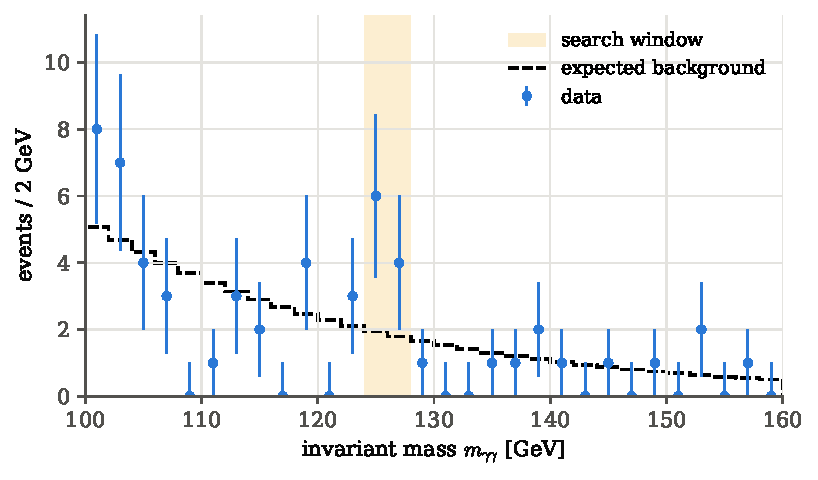
\includegraphics[width=0.82\linewidth]{figures/ch04/bump_spectrum.pdf}
\caption{A simulated diphoton mass spectrum. The dots are the observed counts
per $2\,$GeV bin, the dashed staircase is the background we expect with no new
particle, and the shaded band is the two-bin window $124$--$128\,$GeV where
the excess sits. The error bars are $\sqrt{n}$ and are drawn only to guide the
eye; the pitfall at the end of \cref{4a:sec:bump} explains why they must not be used
to judge the excess.}
\label{4a:fig:bump-spectrum}
\end{figure}

The first thing we can compute is not whether the particle exists. It is how
surprising the bump would be \emph{if nothing new were there}. That is weaker
than what we want to know, but we can compute it exactly, and every discovery
claim in physics starts with it.

\paragraph{The question in words.}
Before any formula, we can list the three things we need.
\begin{enumerate}[label=\arabic*.]
  \item A hypothesis precise enough to \emph{predict} the data, with no knob
        left to turn. ``Only background'' is such a hypothesis: the dashed line
        tells us the Poisson mean of every bin.
  \item One number computed from the data that is large when there is a
        signal and small when there is not. Here, the count in the window.
  \item The answer to: if only background were present, how often would that
        number come out at least as large as the one we saw?
\end{enumerate}

\subsection{The null hypothesis is the one whose predictions we know}
\label{4a:sec:null}

Every test starts by splitting the possible values of an unknown parameter
into two sets, one for each hypothesis. This is the same for a particle search
and for a medical trial. \mainref{p.~149} opens with rats: expose one group to
asbestos, leave another unexposed, and compare the disease rates. Either the
two rates are the same, or they are not. In the bump, the unknown parameter is
the expected number $s$ of signal events in the window, and physics allows
any $s\ge0$. Writing $\theta$ for the parameter and $\Theta$ for the set of all
its allowed values, the two hypotheses are two disjoint sets that together
cover $\Theta$:
\begin{equation}
  \Hnull:\ \theta\in\Theta_0
  \qquad\text{versus}\qquad
  \Halt:\ \theta\in\Theta_1,
  \qquad \Theta_0\cup\Theta_1=\Theta,\quad \Theta_0\cap\Theta_1=\varnothing .
  \label{4a:eq:partition}
\end{equation}
For the bump, $\theta=s$, $\Theta=[0,\infty)$, $\Theta_0=\{0\}$ and
$\Theta_1=(0,\infty)$. For the rats, $\theta$ is the difference of the two
disease rates, $\Theta_0=\{0\}$, and $\Theta_1$ is every nonzero difference.

The two hypotheses are not on an equal footing, and the asymmetry is the whole
point. $\Hnull$ is the \newterm{null hypothesis}: the data came about by
chance alone, from processes we already understand. We treat it this way
\emph{because we know its probability distribution}. With $s=0$ the count in
every bin is Poisson with a known mean, and we can compute, or simulate, the
probability of any outcome. The alternative $\Halt$ is a whole family: every
$s>0$, every possible mass and width of the new particle, each predicting
something different. We cannot compute ``the'' probability of the data under
$\Halt$ without first choosing one of its members.

So we test ``chance alone'' not because we believe it, but because it is the
one case whose probability density we actually know. A test therefore runs in
the \emph{prediction} direction of \cref{ch:01}. We start from the one
situation we can simulate, $\Hnull$, and ask what outcomes it produces and how
often. Only then do we compare with what we saw.

\paragraph{The question a test asks.}
Suppose $\Hnull$ is true. Would a result like the one we got, or even more in
this direction, then be a reasonable thing to expect?

If the answer is ``hardly ever'', the data give us evidence against $\Hnull$.
If the answer is ``quite often'', they do not. Notice what we did \emph{not}
ask: how probable $\Hnull$ is. That question runs in the inference direction
and needs Bayes' theorem, and we come back to it in
\cref{4a:sec:not-posterior} and \cref{ch:05}.

\subsection{Test statistic, rejection region, critical value}
\label{4a:sec:rejection}

Data sets are long lists of numbers, and we cannot compare lists directly.
We compress the data $\bm x$ into one number, the \newterm{test statistic}
$T(\bm x)$ \unpack{a function of the data alone, chosen to be large when
$\Halt$ is true}. For the bump, $T$ is the count $n$ in the window. Large $n$
points to a signal, and $n$ near the expected background points to nothing.

A test is then a rule for turning $T$ into a decision. We choose a set of
outcomes, the \newterm{rejection region} $R$, and agree in advance
\mainref{(10.2)}, \srcref{Cowan}{\S4.1}:
\begin{equation}
  \bm x\in R\ \Longrightarrow\ \text{reject }\Hnull,
  \qquad
  \bm x\notin R\ \Longrightarrow\ \text{retain }\Hnull,
  \qquad
  R=\{\bm x:\ T(\bm x)>c\}.
  \label{4a:eq:rejection}
\end{equation}
The threshold $c$ is the \newterm{critical value}. Cowan calls the rejection
region the \emph{critical region} and its complement the \emph{acceptance
region}. We say ``retain'' rather than ``accept'': not rejecting the null only
means the data did not contradict it, just as a jury that fails to convict
has not proved innocence. The whole problem of testing is to choose a good
$T$ and a sensible $c$. Choosing $c$ is the subject of
\cref{4a:sec:power}; choosing $T$, of \cref{4a:sec:np}.

\mainref{p.~150} adds a warning worth keeping in mind from the start: tests
are for well-defined hypotheses. If the real question is ``how big is the
effect?'', an estimate with a confidence interval answers it better than a
test.

\subsection{The p-value: the tail beyond what we saw}
\label{4a:sec:pvalue-def}

Instead of fixing $c$ in advance and reporting only ``reject'' or ``retain'',
we can report \emph{where} the observed statistic $t_{\rm obs}$ falls in the
null distribution. \Cref{4a:fig:null-tail} shows the picture that the whole
chapter keeps returning to. The curve is $g(t\given\Hnull)$, the sampling
distribution of the test statistic when the null is true. The vertical line is
the value we observed. The shaded area to the right is the probability,
under $\Hnull$, of a result like ours or even more in the direction that
signals $\Halt$. That area is the p-value.

\begin{figure}[htbp]
\centering
\begin{tikzpicture}
\begin{axis}[
  width=11cm, height=5.2cm,
  domain=0:14, samples=200,
  xmin=0, xmax=14, ymin=0, ymax=0.3,
  axis lines=left, xlabel={test statistic $t$}, ylabel={$g(t\given H_0)$},
  xtick={0,2,4,6,8,10,12,14}, ytick=\empty,
  clip=false]
  \addplot[name path=f, formblue, very thick] {x^2*exp(-x)/2};
  \path[name path=axis] (axis cs:0,0) -- (axis cs:14,0);
  \addplot[fibreorange!70, opacity=0.8] fill between[of=f and axis, soft clip={domain=6.5:14}];
  \draw[bdryred, thick] (axis cs:6.5,0) -- (axis cs:6.5,0.17);
  \node[anchor=south, bdryred, font=\small] at (axis cs:6.5,0.17) {$t_{\rm obs}$};
  \node[anchor=west, font=\small, align=left] at (axis cs:8.6,0.085)
       {shaded area $=p$\\$=\Prob(T\ge t_{\rm obs}\given H_0)$};
  \draw[->, black!60] (axis cs:8.5,0.075) -- (axis cs:7.5,0.025);
  \node[anchor=west, font=\small, formblue] at (axis cs:3.3,0.25)
       {typical under $H_0$};
  \draw[->, thick, fibreorange!80!black] (axis cs:9.5,0.20) -- (axis cs:13.5,0.20);
  \node[anchor=south, font=\small, fibreorange!80!black] at (axis cs:11.5,0.205)
       {direction of $H_1$};
\end{axis}
\end{tikzpicture}
\caption{The p-value as a tail area. The blue curve is the distribution of the
test statistic in a world where only chance operates. The observed value sits
at the red line. The orange tail collects every outcome at least as extreme,
in the direction the alternative predicts. A small tail means our result would
be rare if the null were true.}
\label{4a:fig:null-tail}
\end{figure}

\begin{workdef}[p-value]
For a test that rejects $\Hnull$ when $T$ is large, and a simple null
$\Theta_0=\{\theta_0\}$, the \newterm{p-value} of the observed data is
\[
  p=\Prob_{\theta_0}\bigl(T\ge t_{\rm obs}\bigr)
\]
\unpack{the probability, computed as if $\Hnull$ were true, of a test
statistic at least as large as the one observed}. It is computed from
$\Hnull$ alone and is \emph{not} the probability that $\Hnull$ is true.
Operationally: simulate many data sets under $\Hnull$, compute $T$ for each,
and count the fraction with $T\ge t_{\rm obs}$
\mainref{Thm~10.12}, \srcref{Cowan}{\S4.5}.
\end{workdef}

Three features of the definition matter.
\begin{itemize}[itemsep=1pt,leftmargin=1.2em]
  \item The p-value is a probability of \emph{data}, not of hypotheses. The
        null value $\theta_0$ sits in the subscript as a fixed assumption.
  \item It counts the observed value itself and everything beyond it. The words
        ``or even more in this direction'' are needed because, once the data
        are rich enough, the probability of getting exactly $t_{\rm obs}$ is
        tiny under any hypothesis, so it cannot measure surprise on its own.
  \item It needs a \emph{direction}. We must say in advance which outcomes
        count as more extreme. \Cref{4a:sec:sides} shows that this choice is
        part of the question.
\end{itemize}

\subsection{The p-value of a Poisson excess}
\label{4a:sec:poisson-p}

\emph{What we need.} Under the null, the count $N$ in the window adds up many
rare, independent background events, so it is a Poisson variable
(\cref{ch:02}). Its mean $b$ is the expected background in the window. So the
first step is to find $b$, and the second is to add up the Poisson tail.

\emph{The expected background.} Take the background to be
exponential in mass, $f(m)\propto e^{-(m-m_0)/L}$ with $m_0=100\,$GeV, decay
length $L=25\,$GeV, and total expectation $B=\FourABumpBtot$ over the range
$[100,160]\,$GeV. Its cumulative distribution on this range is
$F(m)=\bigl(1-e^{-(m-m_0)/L}\bigr)/\bigl(1-e^{-60/L}\bigr)$, and the expected
background in the window is
\begin{align}
  b &\eqby{1} B\,\bigl[F(128)-F(124)\bigr] \notag\\
    &\eqby{2} B\,\frac{e^{-24/25}-e^{-28/25}}{1-e^{-60/25}}
     = \FourABumpBtot\times\frac{0.3829-0.3263}{1-0.0907}
     \approx \FourABumpB .
  \label{4a:eq:bwin}
\end{align}
\begin{explain}
  \item The expected number of background events in a window is the total
        expectation times the fraction of the background probability that
        falls inside the window.
  \item Insert $F$. The denominators cancel between $F(128)$ and $F(124)$,
        and the ones cancel in the difference.
\end{explain}

\emph{The tail.} With $b$ in hand, the p-value of observing $n_{\rm obs}$
events is the probability that a Poisson count with mean $b$ comes out at
$n_{\rm obs}$ or above \srcref{Cowan}{(4.38)}:
\begin{align}
  p=\Prob(N\ge n_{\rm obs}\given\Hnull)
  &\eqby{1} \sum_{n=n_{\rm obs}}^{\infty}\Prob(N=n\given s=0) \notag\\
  &\eqby{2} \sum_{n=n_{\rm obs}}^{\infty}\frac{b^n e^{-b}}{n!} \notag\\
  &\eqby{3} 1-\sum_{n=0}^{n_{\rm obs}-1}\frac{b^n e^{-b}}{n!} .
  \label{4a:eq:poisson-p}
\end{align}
\begin{explain}
  \item The events $\{N=n\}$ for different $n$ are disjoint, so their
        probabilities add. The direction is ``upwards'', because a signal
        can only add events.
  \item Under $\Hnull$ the count is Poisson with mean $b$.
  \item The Poisson probabilities sum to one, because
        $\sum_{n\ge0}b^n/n!=e^{b}$. So the infinite upper tail equals one
        minus a \emph{finite} sum, which is what we actually evaluate.
\end{explain}

\paragraph{Example: our bump.}
In the two-bin window there are $n_{\rm obs}=\FourABumpN$ events on an
expected background of $b=\FourABumpB$. The finite sum in
\eqref{4a:eq:poisson-p} runs over $n=0,\dots,9$, and
\[
  p=\Prob(N\ge\FourABumpN\given b=\FourABumpB)=\FourABumpP .
\]
About one background-only experiment in $190$ would give a window at least
this full. \Cref{4a:fig:bump-null} shows the null distribution of the window
count with this tail shaded, and the same distribution rebuilt from $10^6$
simulated background-only experiments.

\begin{figure}[htbp]
\centering
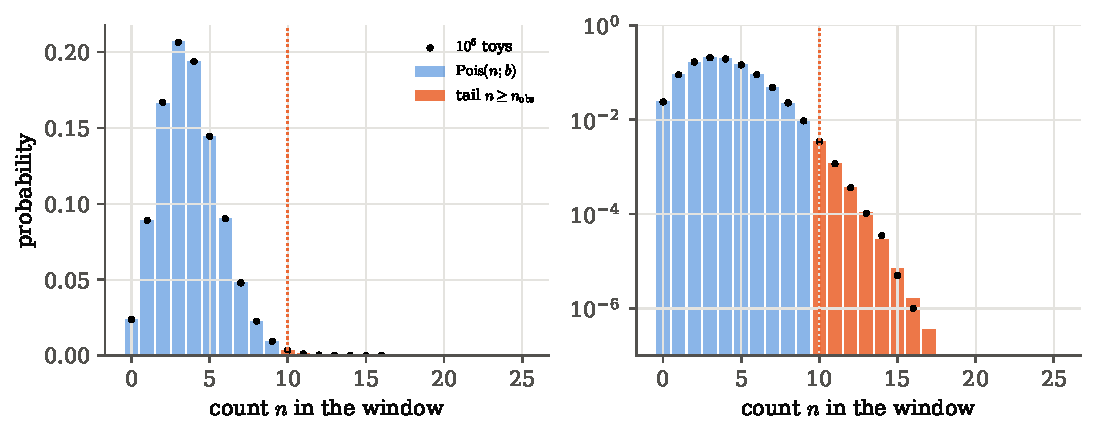
\includegraphics[width=\linewidth]{figures/ch04/bump_null.pdf}
\caption{The null distribution of the window count, $\mathrm{Pois}(n;b)$ with
$b=\FourABumpB$, on a linear scale (left) and a log scale (right). The orange
bars are the outcomes at least as large as the observed $n_{\rm obs}=\FourABumpN$,
and their total height is the p-value. The black dots are the frequencies in
a million simulated background-only experiments. They follow the bars even far
out in the tail, where the log scale is needed to see them.}
\label{4a:fig:bump-null}
\end{figure}

\paragraph{Example: Cowan's peak.}
\srcref{Cowan}{p.~60, Fig.~4.3} shows a histogram with a peak where two bins
contain $n_{\rm obs}=11$ entries on an expected background of $b=3.2$. The
same formula gives
\[
  p=1-\sum_{n=0}^{10}\frac{3.2^n e^{-3.2}}{n!}=\FourACowanPone ,
\]
the value $5.0\times10^{-4}$ quoted there. Fewer than one background-only
histogram in two thousand would have such a full pair of bins \emph{at that
location}. The last three words matter: a peak could have appeared anywhere
in the histogram, and \srcref{Cowan}{p.~61} points out that the fair
question is how often a peak this improbable appears in \emph{any} bin. That
is the look-elsewhere effect, treated in the second part of the chapter.

\paragraph{Example: a few events on almost no background, and a background we
do not quite know.}
The p-value is computed \emph{entirely} from the null model, so an error in
the expected background goes straight into it. Suppose we expect $b=0.5$
background events and observe $n_{\rm obs}=5$ \srcref{Cowan}{p.~59}. Then
\eqref{4a:eq:poisson-p} gives $p=\FourACowanPtwo$. If the background estimate
is off and the true value is $b=0.8$, the same five events give
$p=\FourACowanPthree$, almost ten times larger. A modest error in the
background has turned a striking result into a much less striking one. This is
why every real search spends most of its effort on the background estimate,
and quotes p-values for a range of plausible $b$.

\subsection{Python: exact tail and simulated tail}
\label{4a:sec:bump-python}

\Cref{4a:lst:bump} shows the lines of \pyname{code/ch04/01_bump_pvalue.py}
that compute the p-value twice.

\pyfile[firstline=39,lastline=52,label={4a:lst:bump}]{code/ch04/01_bump_pvalue.py}{The window count, its exact Poisson p-value, and a Monte Carlo p-value}

The mask \pyname{win} picks the two bins between $124$ and $128\,$GeV, and
summing the expected background and the observed counts over it gives $b$
and $n_{\rm obs}$. The function \pyname{stats.poisson.sf(k, b)} is the
\emph{survival function} $\Prob(N>k)$, so asking for
\pyname{sf(n_win - 1, b_win)} gives $\Prob(N\ge n_{\rm obs})$, exactly the
last line of \eqref{4a:eq:poisson-p}. The off-by-one is the most common bug
in this computation: $\Prob(N>n_{\rm obs})$ leaves out the observed value
itself.

The Monte Carlo version is the definition of the p-value turned into code, and
it does not use the formula at all. It draws $M=10^6$ background-only
experiments, each a single Poisson count with mean $b$, and counts the
fraction at least as large as the observation. It finds $p=\FourABumpPmc$,
with a binomial standard error of $\sqrt{p(1-p)/M}=\FourABumpPmcErr$, in
agreement with the exact value $\FourABumpP$. Here the simulation is overkill,
because the tail sum is exact. But when the test statistic is complicated and
its null distribution has no formula, which is the usual situation in
research, simulation is the only option.

The simulated data do contain a signal: $\FourABumpStot$ expected events from
a narrow resonance at $126\,$GeV. The test does not know this. With these
numbers it cannot tell a real signal of this size from a lucky fluctuation
with much confidence. \Cref{4a:sec:power} asks how large a signal must be
before a test catches it reliably.

\begin{pitfall}[The $\sqrt{n}$ error bar answers the wrong question]
It is tempting to write the observation as $n\pm\sqrt n$, subtract the
background, and count standard deviations. For five events on $b=0.5$ this
gives $4.5\pm2.2$, ``only two standard deviations'' from zero, even though
$p=\FourACowanPtwo$ says the excess is very unusual \srcref{Cowan}{p.~60}.
The error bar $\sqrt n$ describes how a Poisson variable \emph{with mean $n$}
fluctuates down. The p-value asks how a Poisson variable \emph{with mean $b$}
fluctuates up, and only the second question is posed by the null. For our
bump, $(n-b)/\sqrt n=\FourABumpZwrong$ and $(n-b)/\sqrt b=\FourABumpZnaive$,
while the exact tail corresponds to $\FourABumpZ$ Gaussian standard
deviations (the conversion is explained in \cref{4a:sec:ztable}). Neither
shortcut is right for small counts. Compute the tail.
\end{pitfall}

Two practical lessons from \srcref{Cowan}{p.~61} complete the recipe. The
window must be fixed before we look at the data, with a width of a few times
the mass resolution; widening or shifting it to make the excess look better
destroys the meaning of the p-value, because the null distribution was
computed for a fixed window. And the p-value of one window ignores the
other bins, some of which are also a little high or low. A test of the whole
histogram against the background shape is a goodness-of-fit test, the subject
of \cref{4a:sec:gof}.
\section{Which way is ``more extreme''? Sides, and the stopping rule}
\label{4a:sec:sides}

A coin is tossed $N=20$ times and comes up heads $n_h=17$ times
\srcref{Cowan}{p.~58}. A fair coin gives $10$ heads on average, so $17$ looks
suspicious. To turn the suspicion into a p-value we must say which other
outcomes are ``at least as extreme'' as $17$ heads. The answer is not a
technicality. It depends on what we were worried about before we tossed, and,
more surprisingly, on how we decided when to stop tossing. The coin is small
enough that we can do every sum by hand and see both effects directly.

\paragraph{The question in words.}
\begin{enumerate}[label=\arabic*.]
  \item Which alternative are we guarding against: a coin biased towards
        heads, or a coin biased either way?
  \item Given that choice, which outcomes count as ``this, or even more in
        this direction''?
  \item Did the experimenter fix the number of tosses in advance, or stop for
        some other reason? The imaginary repetitions that the p-value averages
        over must follow the same plan.
\end{enumerate}

\subsection{Simple and composite hypotheses, one and two sides}
\label{4a:sec:simple-composite}

A hypothesis that fixes the distribution of the data completely is
\newterm{simple}. ``The coin is fair'', $p=\tfrac12$, is simple: it predicts
$n_h\sim\mathrm{Binomial}(20,\tfrac12)$ \unpack{the number of successes in $20$
independent tries, each with success probability $\tfrac12$}. A hypothesis
that leaves at least one parameter free is \newterm{composite}, for example
$p\le\tfrac12$ or $p\neq\tfrac12$ \mainref{p.~151}, \srcref{Cowan}{\S4.1}.

The alternative decides the shape of the rejection region.
\begin{itemize}
  \item A \newterm{two-sided test}, $\Hnull:\theta=\theta_0$ versus
        $\Halt:\theta\neq\theta_0$, guards against departures in both
        directions. For the coin, very many heads and very few heads are both
        evidence of bias, and a sensible statistic is the distance from the
        expected value, $T=\abs{n_h-N/2}$.
  \item A \newterm{one-sided test}, $\Hnull:\theta\le\theta_0$ versus
        $\Halt:\theta>\theta_0$ (or the mirror image), guards against a
        departure in one direction only. If the only suspicion is a coin loaded
        towards heads, then $T=n_h$ and only large values count.
\end{itemize}
In both cases the test statistic is built to be \emph{large when $\Halt$ is
true}, so the rejection region is always ``$T$ large'' and the p-value is always
an upper tail of $T$. The direction lives in the choice of $T$.
\Cref{4a:fig:sides} shows the two rejection regions for a statistic that is
standard normal under the null, with the same total probability $\alpha=0.05$
in each: all of it in one tail beyond $z=\FourAPzZfivepct$, or half in each
tail beyond $\pm\FourAPzZfivepctTwo$.

\begin{figure}[htbp]
\centering
\begin{tikzpicture}
\pgfplotsset{fouraSides/.style={width=6.4cm, height=4.2cm, domain=-3.6:3.6,
  samples=160, xmin=-3.6, xmax=3.6, ymin=0, ymax=0.47, axis lines=left,
  ytick=\empty, xtick={-2,0,2}, xlabel={$z$}}}
\begin{axis}[fouraSides, title={\small one-sided: $H_1:\theta>\theta_0$}]
  \addplot[name path=g, formblue, thick] {exp(-x^2/2)/sqrt(2*pi)};
  \path[name path=ax] (axis cs:-3.6,0) -- (axis cs:3.6,0);
  \addplot[fibreorange!75] fill between[of=g and ax, soft clip={domain=1.645:3.6}];
  \draw[bdryred] (axis cs:1.645,0) -- (axis cs:1.645,0.30);
  \node[anchor=south, font=\small, bdryred] at (axis cs:1.645,0.30) {$1.645$};
  \node[anchor=south west, font=\small] at (axis cs:2.0,0.07) {$\alpha$};
\end{axis}
\begin{axis}[fouraSides, xshift=7cm, title={\small two-sided: $H_1:\theta\neq\theta_0$}]
  \addplot[name path=g, formblue, thick] {exp(-x^2/2)/sqrt(2*pi)};
  \path[name path=ax] (axis cs:-3.6,0) -- (axis cs:3.6,0);
  \addplot[fibreorange!75] fill between[of=g and ax, soft clip={domain=1.96:3.6}];
  \addplot[fibreorange!75] fill between[of=g and ax, soft clip={domain=-3.6:-1.96}];
  \draw[bdryred] (axis cs:1.96,0) -- (axis cs:1.96,0.30);
  \draw[bdryred] (axis cs:-1.96,0) -- (axis cs:-1.96,0.30);
  \node[anchor=south, font=\small, bdryred] at (axis cs:1.96,0.30) {$1.96$};
  \node[anchor=south, font=\small, bdryred] at (axis cs:-1.96,0.30) {$-1.96$};
  \node[anchor=south west, font=\small] at (axis cs:2.3,0.05) {$\alpha/2$};
  \node[anchor=south east, font=\small] at (axis cs:-2.3,0.05) {$\alpha/2$};
\end{axis}
\end{tikzpicture}
\caption{The same total probability $\alpha=0.05$ placed in one tail (left)
or split between two tails (right) of a standard normal null distribution. The
one-sided test rejects sooner in the direction it cares about, at $1.645$
instead of $1.96$, and never rejects in the other direction.}
\label{4a:fig:sides}
\end{figure}

\paragraph{Example: 17 heads in 20 tosses.}
The binomial probability of $k$ heads for a fair coin is
$\binom{20}{k}2^{-20}$, and $2^{20}=1\,048\,576$. If we only feared a coin
loaded towards heads, the p-value is
\begin{align}
  p_{\text{one}}=\Prob(n_h\ge17\given p=\tfrac12)
  &\eqby{1} \frac{1}{2^{20}}\Bigl[\tbinom{20}{17}+\tbinom{20}{18}+\tbinom{20}{19}+\tbinom{20}{20}\Bigr] \notag\\
  &\eqby{2} \frac{1140+190+20+1}{1\,048\,576}=\frac{1351}{1\,048\,576}
   \approx\FourACoinPone .
  \label{4a:eq:coin-one}
\end{align}
\begin{explain}
  \item Add the probabilities of the disjoint outcomes $17,18,19,20$ heads.
  \item $\binom{20}{17}=\binom{20}{3}=\frac{20\cdot19\cdot18}{6}=1140$,
        $\binom{20}{18}=\binom{20}{2}=190$, $\binom{20}{19}=20$,
        $\binom{20}{20}=1$.
\end{explain}
If any bias counts, the outcomes at least as far from $10$ as $17$ are
$n_h\in\{0,1,2,3\}\cup\{17,\dots,20\}$, that is $\abs{n_h-10}\ge7$. The
binomial with $p=\frac12$ is symmetric, $\binom{20}{k}=\binom{20}{20-k}$, so
the lower tail equals the upper one and
\[
  p_{\text{two}}=\Prob\bigl(\abs{n_h-10}\ge7\given p=\tfrac12\bigr)
  =2\,p_{\text{one}}=\frac{2702}{1\,048\,576}\approx\FourACoinPtwo ,
\]
the value $0.0026$ of \srcref{Cowan}{p.~58}. \Cref{4a:fig:coin-sides} shows
the eight outcomes that enter. The two answers differ by a factor of two, and
both are correct answers to different questions.

\begin{figure}[htbp]
\centering
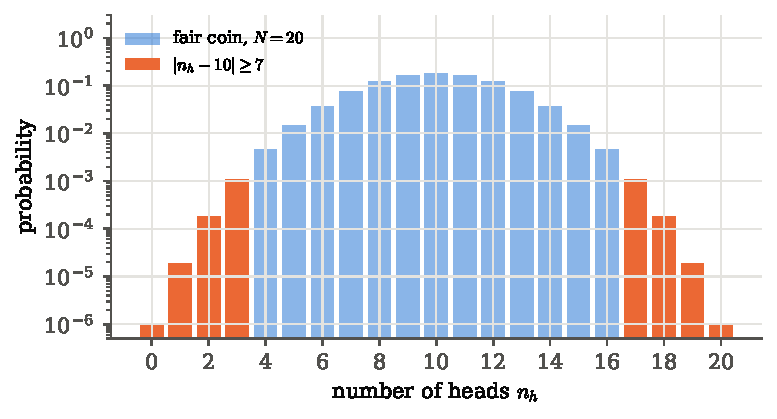
\includegraphics[width=0.78\linewidth]{figures/ch04/coin_sides.pdf}
\caption{The binomial distribution of the number of heads in $20$ tosses of a
fair coin, on a logarithmic vertical scale so that the thin tails show. The orange
bars are the outcomes at least as far from $10$ as the
observed $17$, on either side. Their total is the two-sided p-value; the four
bars on the right alone give the one-sided one.}
\label{4a:fig:coin-sides}
\end{figure}

\paragraph{A composite null.}
For a one-sided composite null, the p-value is the tail at the boundary of the
null, so the composite test reduces to the simple test at $\theta_0$. To see
why, pose the one-sided coin question with the composite null
$\Hnull:p\le\frac12$, where $p$ is now the probability of heads. The problem is
that every $p$ in $\Theta_0$ gives a different tail probability
$\Prob_p(n_h\ge17)$. The rule \mainref{Thm~10.12} is to report the largest of
them, $\sup_{\theta\in\Theta_0}\Prob_\theta(T\ge t_{\rm obs})$, so that the
number is honest for every member of the null. The tail $\Prob_p(n_h\ge17)$
grows with $p$, because a coin more inclined to heads gives more heads. So the
largest tail is reached at the boundary $p=\frac12$, and the answer is again
$\FourACoinPone$. The boundary value is the member of the null hardest to tell
apart from the alternative.

\paragraph{When the null distribution is not symmetric.}
A skewed null needs a convention for its two-sided p-value. For the fair coin,
``twice the one-sided tail'' and ``everything at least as far from the mean''
agree. For a skewed null, such as a Poisson with small mean, they do not, and
we must choose one of two rules: either double the
smaller tail, or add the probabilities of all outcomes that are no more
probable than the one observed. In searches for new physics the question is
almost always one-sided anyway, because a signal can only add events.

\begin{pitfall}[Choosing the side after seeing the data]
The side is part of the question, so it must be chosen before looking at the
data. Deciding on a one-sided test \emph{because} the excess came out
upwards halves the p-value without any new evidence. Under the null this
procedure rejects whenever either tail holds $\alpha$ of the probability, so
its true type I error rate is $2\alpha$, not $\alpha$.
\end{pitfall}

\subsection{The same data, different p-values: the stopping rule}
\label{4a:sec:stopping}

The same data can give different p-values, depending on how the experimenter
decided when to stop. The reason is in what the p-value asks for: the
probability of outcomes ``like this or more extreme'' in \emph{repetitions of
the experiment}. Those repetitions never happened. We imagine them, or, in the
blunt words of \srcref{Lambert}{\S2.8}, to test a hypothesis we ``invent
fictitious samples''. Lambert's example: if we hypothesise that heights are
normal with mean $1.55\,$m and standard deviation $0.3\,$m and meet one person
of $2.5\,$m, the p-value is the probability of meeting someone \emph{at least}
$2.5\,$m tall, although nobody taller was observed. To imagine the repetitions
we must know the plan that produced the data, and the data alone do not tell
us.

\emph{The data.} \srcref{Kruschke}{\S11.1} gives the example. A coin shows
$z=7$ heads in $N=24$ tosses. Is it fair? We take two possible plans in turn.

\paragraph{Plan A: the number of tosses was fixed at $N=24$.}
Then the random quantity is the number of heads $z$, it is
$\mathrm{Binomial}(24,\frac12)$ under the null, and few heads is the extreme
direction:
\[
  p_A=\Prob(z\le7\given N=24)=\sum_{k=0}^{7}\binom{24}{k}2^{-24}=\FourAKrFixN .
\]

\paragraph{Plan B: the experimenter tossed until the seventh head.}
Now $z=7$ is fixed by design and the random quantity is the number of tosses
$N$ it took. Needing \emph{many} tosses to collect seven heads is the sign of
a tail-heavy coin, so the extreme direction is $N\ge24$. The event $\{N\ge24\}$
is the same as ``at most six heads in the first $23$ tosses'':
\begin{align}
  p_B=\Prob(N\ge24\given z=7)
  &\eqby{1} \Prob\bigl(\text{at most 6 heads in the first 23 tosses}\bigr) \notag\\
  &\eqby{2} \sum_{k=0}^{6}\binom{23}{k}2^{-23}
   = \FourAKrFixZ .
  \label{4a:eq:fixz}
\end{align}
\begin{explain}
  \item The seventh head arrives at toss $24$ or later exactly when the first
        $23$ tosses contain six heads or fewer.
  \item The first $23$ tosses of a fair coin are
        $\mathrm{Binomial}(23,\frac12)$, whatever happens afterwards.
\end{explain}
The distribution of $N$ itself is the negative binomial of \cref{ch:02}: the
$n$-th toss is the seventh head when it is a head and the previous $n-1$ tosses
hold exactly six heads, so $\Prob(N=n)=\binom{n-1}{6}2^{-n}$.
\Cref{4a:fig:stopping} shows the two clouds of imaginary outcomes side by side.

\begin{figure}[htbp]
\centering
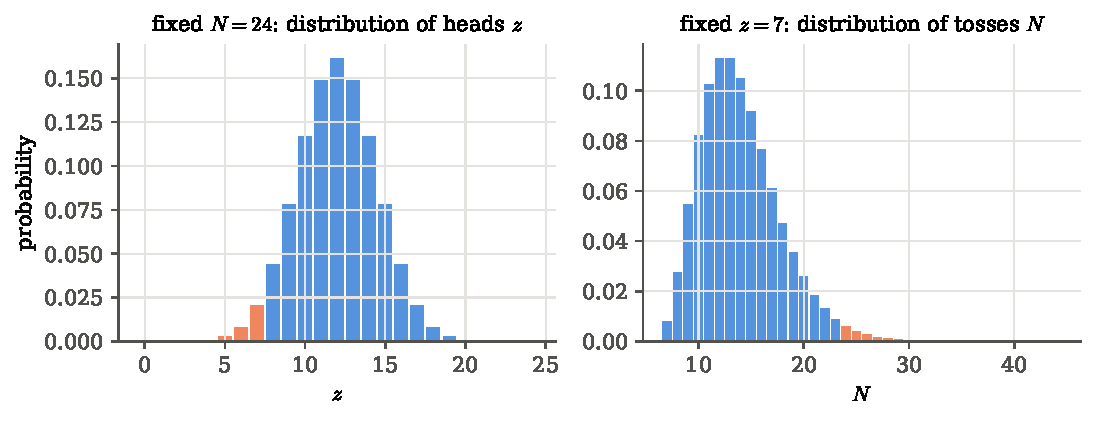
\includegraphics[width=\linewidth]{figures/ch04/stopping_rules.pdf}
\caption{Two plans that can produce the same record of $7$ heads in $24$
tosses. Left: with $N=24$ fixed, the random quantity is the number of heads,
and its lower tail $z\le7$ (orange) is the p-value. Right: when tossing stops
at the seventh head, the random quantity is the number of tosses, and its upper
tail $N\ge24$ (orange) is the p-value. The observed data are identical; the
imagined repetitions are not.}
\label{4a:fig:stopping}
\end{figure}

\emph{What the two plans say.} The very same sequence of tosses is ``not
significant'' under one plan and ``significant'' under the other. With the
conventional two-tailed threshold, which puts $2.5\%$ in each tail, plan A
gives $p_A=\FourAKrFixN$, above $0.025$, and plan B gives $p_B=\FourAKrFixZ$,
below it.
\srcref{Kruschke}{p.~309} adds two more plans. If the experimenter tossed for
a fixed length of time, so that $N$ itself is random (Poisson), the p-value is
$0.024$. If a second coin was tested in the same study and the question is
whether \emph{either} coin looks this extreme, the chance that at least one of
two independent fixed-$N$ experiments reaches the tail is
$1-(1-p_A)^2\approx2p_A$, which is the $0.063$ found there. The last case is
our first taste of the look-elsewhere effect.

\paragraph{Example: Cowan's stopping rule.}
\srcref{Cowan}{p.~58} tells the same story with the 17 heads in 20 tosses.
Suppose the plan was ``toss until there are at least three heads and at least
three tails'', and the stopping happened at toss $20$ (with $17$ heads and
$3$ tails). Now the extreme outcomes are those that need $20$ tosses or more:
\begin{align}
  \Prob(N_{\rm stop}\ge20)
  &\eqby{1} \Prob\bigl(\text{after 19 tosses, heads}\le2\ \text{or tails}\le2\bigr) \notag\\
  &\eqby{2} 2\,\Prob\bigl(\mathrm{Binomial}(19,\tfrac12)\le2\bigr) \notag\\
  &\eqby{3} 2\,\frac{\binom{19}{0}+\binom{19}{1}+\binom{19}{2}}{2^{19}}
   = \frac{2\,(1+19+171)}{524\,288}\approx\FourACowStop .
  \label{4a:eq:cowan-stop}
\end{align}
\begin{explain}
  \item We are still tossing after toss $19$ exactly when one of the two
        faces has appeared at most twice so far.
  \item The two events are disjoint (both at most $2$ would mean at most $4$
        tosses, not $19$), so their probabilities add, and by symmetry they
        are equal.
  \item Binomial sum with $\binom{19}{2}=171$ and $2^{19}=524\,288$.
\end{explain}
That is $0.073\%$ instead of the $0.26\%$ of the fixed-$N$ plan
\srcref{Cowan}{p.~58}. Cowan's resolution is a convention: always interpret
``similar experiments'' as experiments with the same number of observations.
It is arbitrary, but it makes a reported p-value unambiguous.

\paragraph{Python.}
The script \pyname{code/ch04/02_sides_and_stopping.py} evaluates every tail
sum above with \pyname{scipy.stats.binom} and then checks each one by running
the stated protocol many times.

\pyfile[firstline=34,lastline=52]{code/ch04/02_sides_and_stopping.py}{Two stopping plans, and Cowan's rule, simulated}

For plan B it uses the fact that the number of tails before the seventh head is
a negative binomial variable, \pyname{rng.negative_binomial(7, 0.5)}, so the
total number of tosses is seven plus that. For Cowan's rule it simply tosses:
$200\,000$ sequences of $60$ tosses, running totals of heads and tails with
\pyname{np.cumsum}, and the first toss at which both totals reach three. The
simulations give $\FourAKrFixNMC$, $\FourAKrFixZMC$ and $\FourACowStopMC$
against the exact $\FourAKrFixN$, $\FourAKrFixZ$ and $\FourACowStop$, and
$\FourACoinPtwoMC$ against $\FourACoinPtwo$ for the two-sided coin test.

\begin{keyidea}[A p-value depends on the outcomes that did not happen]
A p-value is a sum over imaginary repetitions of the experiment. Which
repetitions are imagined depends on the plan: the alternative we guard against
(one or two sides), when the experimenter would have stopped, and how many
other places or coins we would also have looked at. Change the plan and the
p-value changes, even if the data do not.
\end{keyidea}

A Bayesian analysis does not have this problem, because it uses only the
probability of the data actually observed. In plan A that probability is
$\binom{24}{7}p^7(1-p)^{17}$ and in plan B it is $\binom{23}{6}p^7(1-p)^{17}$.
As functions of the coin's bias $p$, the two likelihoods differ only by a
constant factor, which cancels in Bayes' theorem. Any inference built from the
likelihood alone therefore reaches the same conclusion under both plans
\srcref{Kruschke}{\S11.1.7}. The p-value, which sums over outcomes that were
not observed, does not. We take this up in \cref{ch:05}. For now the practical
rule is Cowan's: fix the plan in advance, state it, and compute the p-value for
that plan.
\section{Two ways to be wrong: size, power and how much data we need}
\label{4a:sec:power}

A p-value tells us how surprising one data set is. Before the experiment runs,
we face a different pair of questions. How often will our procedure cry
``discovery'' when there is nothing there? And if there \emph{is} something
there, of a given size, how often will we catch it? The first number protects
the field from false claims. The second tells us whether the experiment is
worth building. A detector that can only see a signal one time in ten is a
bad investment, however careful the analysis.

\mainref{p.~150} offers the legal trial as a model. The defendant is presumed
innocent, the null, and is convicted only if the evidence is strong. Two
mistakes are possible: convicting an innocent person, and acquitting a guilty
one. A court that never convicts makes no mistakes of the first kind, and is
useless. There is a trade-off, and it can be put into numbers.

\paragraph{The question in words.}
\begin{enumerate}[label=\arabic*.]
  \item If the null is true, what is the probability that the test rejects it?
  \item If a particular alternative is true, what is the probability that the
        test rejects the null?
  \item How do both depend on the critical value and on the amount of data,
        and how large must an experiment be to catch an effect of a given size?
\end{enumerate}

\subsection{Type I and type II errors}
\label{4a:sec:errors}

Every test ends in one of four situations \mainref{Table~10.1}:
\begin{center}
\begin{tabular}{lcc}
\toprule
 & retain $\Hnull$ & reject $\Hnull$ \\
\midrule
$\Hnull$ true & correct & \newterm{type I error} (false alarm) \\
$\Halt$ true & \newterm{type II error} (missed signal) & correct \\
\bottomrule
\end{tabular}
\end{center}
Cowan calls them errors of the first and second kind \srcref{Cowan}{\S4.1}.
Picture the test statistic $t$ with its two sampling distributions,
$g(t\given\Hnull)$ and $g(t\given\Halt)$, and a cut $t_{\rm cut}$ above which
we reject (\cref{4a:fig:alpha-beta}). The probability of a type I error is the
area of the null distribution above the cut, and the probability of a type II
error is the area of the alternative below it \srcref{Cowan}{(4.1)--(4.2)}:
\begin{equation}
  \alpha=\int_{t_{\rm cut}}^{\infty}g(t\given\Hnull)\,\dd t,
  \qquad
  \beta_{\rm II}=\int_{-\infty}^{t_{\rm cut}}g(t\given\Halt)\,\dd t .
  \label{4a:eq:alpha-beta}
\end{equation}
Moving the cut to the right shrinks $\alpha$ and grows $\beta_{\rm II}$; moving
it left does the opposite. With a fixed statistic and a fixed amount of data
we cannot shrink both. Only a better statistic (\cref{4a:sec:np}) or more data
separates the two curves.

\begin{figure}[htbp]
\centering
\begin{tikzpicture}
\begin{axis}[
  width=11cm, height=5cm, domain=-3.5:6.5, samples=200,
  xmin=-3.5, xmax=6.5, ymin=0, ymax=0.56, axis lines=left, clip=false,
  xlabel={test statistic $t$}, ytick=\empty, xtick={-2,0,2,4,6}]
  \addplot[name path=h0, formblue, thick] {exp(-x^2/2)/sqrt(2*pi)};
  \addplot[name path=h1, tangentgreen!80!black, thick] {exp(-(x-2.8)^2/2)/sqrt(2*pi)};
  \path[name path=ax] (axis cs:-3.5,0) -- (axis cs:6.5,0);
  \addplot[fibreorange!75] fill between[of=h0 and ax, soft clip={domain=1.645:6.5}];
  \addplot[tangentgreen!30] fill between[of=h1 and ax, soft clip={domain=-3.5:1.645}];
  \draw[bdryred, thick] (axis cs:1.645,0) -- (axis cs:1.645,0.46);
  \node[anchor=south, font=\small, bdryred] at (axis cs:1.645,0.46) {$t_{\rm cut}$};
  \node[font=\small, formblue, anchor=east] at (axis cs:-1.1,0.30) {$g(t\given H_0)$};
  \node[font=\small, tangentgreen!60!black, anchor=west] at (axis cs:3.9,0.30) {$g(t\given H_1)$};
  \node[font=\small, anchor=west] at (axis cs:2.6,0.08) {$\alpha$};
  \draw[black!60] (axis cs:2.6,0.08) -- (axis cs:2.05,0.03);
  \node[font=\small, anchor=east] at (axis cs:0.6,0.08) {$\beta_{\rm II}$};
  \draw[black!60] (axis cs:0.6,0.08) -- (axis cs:1.25,0.06);
  \node[font=\small, anchor=west] at (axis cs:-3.3,0.54) {retain $H_0$};
  \node[font=\small, anchor=east] at (axis cs:6.4,0.54) {reject $H_0$};
\end{axis}
\end{tikzpicture}
\caption{The trade-off behind every test. Blue: the distribution of the
statistic when the null is true; green: when a particular alternative is true.
Everything right of the red cut is rejected. The orange sliver is the
probability of a false alarm, $\alpha$; the pale green region is the
probability of missing the signal, $\beta_{\rm II}$. Sliding the cut trades one
for the other.}
\label{4a:fig:alpha-beta}
\end{figure}

\subsection{The power function}
\label{4a:sec:power-function}

The alternative is rarely a single value, so we want the rejection probability
as a function of the true parameter.

\begin{workdef}[power function, size, level]
The \newterm{power function} of a test with rejection region $R$ is
\[
  \beta(\theta)=\Prob_\theta(\bm X\in R)
\]
\unpack{the probability of rejecting $\Hnull$ when the true parameter is
$\theta$}. For $\theta\in\Theta_1$ it is the probability of a correct
rejection; for $\theta\in\Theta_0$ it is a false-alarm rate. The
\newterm{size} is the worst false-alarm rate,
$\alpha=\sup_{\theta\in\Theta_0}\beta(\theta)$, and a test has
\newterm{level} $\alpha$ if its size is at most $\alpha$ \mainref{Def.~10.1}.
Operationally: simulate data at each $\theta$ and record the fraction of
data sets that the test rejects.
\end{workdef}

A notational trap: Wasserman uses $\beta(\theta)$ for the power, while
\srcref{Cowan}{(4.2)} uses $\beta$ for the type II error probability, so that
Cowan's power is $1-\beta$. Here we use Wasserman's convention and write the type II error
probability at a point $\theta_1\in\Theta_1$ as $\beta_{\rm II}=1-\beta(\theta_1)$.

\paragraph{Example: the one-sided test for a Gaussian mean.}
We take $n$ readings $X_1,\dots,X_n\iid\Normal(\mu,\sigma^2)$ with $\sigma$
known and test $\Hnull:\mu\le0$ against $\Halt:\mu>0$ by rejecting when the
sample mean $\bar X$ exceeds a cut $c$ \mainref{Ex.~10.2}. Recall from
\cref{ch:03} that $\bar X\sim\Normal(\mu,\sigma^2/n)$, so
$Z=\sqrt n(\bar X-\mu)/\sigma$ is standard normal. The power function is
\begin{align}
  \beta(\mu)
  &\eqby{1} \Prob_\mu\bigl(\bar X>c\bigr) \notag\\
  &\eqby{2} \Prob_\mu\Bigl(\frac{\sqrt n(\bar X-\mu)}{\sigma}>\frac{\sqrt n(c-\mu)}{\sigma}\Bigr) \notag\\
  &\eqby{3} \Prob\Bigl(Z>\frac{\sqrt n(c-\mu)}{\sigma}\Bigr) \notag\\
  &\eqby{4} 1-\Phi\Bigl(\frac{\sqrt n(c-\mu)}{\sigma}\Bigr) .
  \label{4a:eq:power-z}
\end{align}
\begin{explain}
  \item Definition of the power function with $R=\{\bar X>c\}$.
  \item Subtract $\mu$ and multiply by $\sqrt n/\sigma>0$ on both sides; this
        does not change the event.
  \item The left-hand side is standard normal whatever $\mu$ is.
  \item $\Phi$ is the standard normal CDF, $\Phi(z)=\Prob(Z\le z)$.
\end{explain}
As $\mu$ increases the argument of $\Phi$ decreases, so $\beta(\mu)$
increases. The largest false-alarm rate over the null region $\mu\le0$ is
therefore at the boundary:
\[
  \alpha=\sup_{\mu\le0}\beta(\mu)=\beta(0)=1-\Phi\Bigl(\frac{\sqrt n\,c}{\sigma}\Bigr)
  \quad\Longrightarrow\quad
  c=\frac{\sigma\,z_\alpha}{\sqrt n},\qquad z_\alpha\equiv\Phi^{-1}(1-\alpha).
\]
So the size-$\alpha$ test rejects when $\sqrt n\,\bar X/\sigma>z_\alpha$:
the sample mean, measured in units of its own standard deviation, must exceed
$z_{0.05}=\FourAPzZfivepct$ for $\alpha=0.05$.

\Cref{4a:fig:power-curves} (left) plots \eqref{4a:eq:power-z} for $n=4$,
$16$ and $64$ with $\sigma=1$, together with simulated rejection rates. All
three curves pass through $\alpha=0.05$ at $\mu=0$: the size does not depend
on $n$, because the cut moves in as $1/\sqrt n$. What depends on $n$ is the
steepness. Quadrupling the data halves the width of $\bar X$'s distribution,
so the curve rises over half the range of $\mu$. In the simulation the rate of
false alarms at $\mu=0$ is $\FourAPowSizeFour$ for $n=4$ and
$\FourAPowSizeSixtyfour$ for $n=64$, both equal to $0.05$ within the
simulation error $\sqrt{0.05\times0.95/20\,000}\approx0.0015$.

\begin{figure}[htbp]
\centering
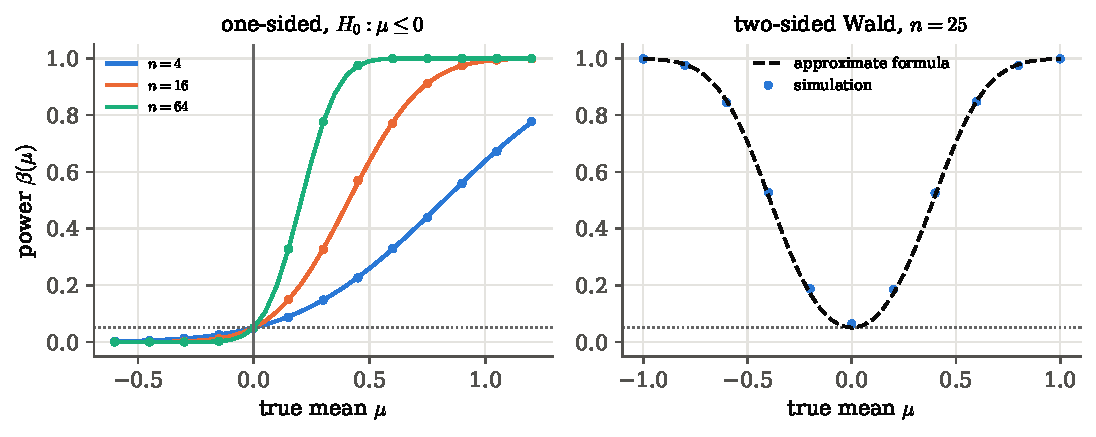
\includegraphics[width=\linewidth]{figures/ch04/power_curves.pdf}
\caption{Power functions. Left: the one-sided test of $\mu\le0$ for three
sample sizes, with the formula as lines and simulated rejection rates as dots.
Every curve crosses the dotted $\alpha=0.05$ line at $\mu=0$ and climbs faster
the more data there are. Right: the two-sided Wald test with $n=25$ and an
estimated standard error; the dashed curve is the approximate formula and the
dots are simulations. The curve is symmetric and bottoms out near $\alpha$ at
$\mu=0$.}
\label{4a:fig:power-curves}
\end{figure}

\paragraph{Example: how many readings do we need?}
Suppose we want power $0.8$ at $\mu_1=0.5\sigma$, with $\alpha=0.05$. Setting
\eqref{4a:eq:power-z} equal to $0.8$ at $\mu=\mu_1$, with $c=\sigma
z_\alpha/\sqrt n$,
\begin{align}
  0.8
  &\eqby{1} 1-\Phi\Bigl(z_\alpha-\frac{\sqrt n\,\mu_1}{\sigma}\Bigr)
  \eqby{2} \Phi\Bigl(\frac{\sqrt n\,\mu_1}{\sigma}-z_\alpha\Bigr) \notag\\
  &\;\Longrightarrow\;
  \frac{\sqrt n\,\mu_1}{\sigma}-z_\alpha \eqby{3} z_{0.2}
  \;\Longrightarrow\;
  n \eqby{4} \Bigl(\frac{(z_\alpha+z_{0.2})\,\sigma}{\mu_1}\Bigr)^2
  =\Bigl(\frac{1.645+0.842}{0.5}\Bigr)^2\approx\FourAPowNreq .
  \label{4a:eq:sample-size}
\end{align}
\begin{explain}
  \item Insert $c=\sigma z_\alpha/\sqrt n$ into $\sqrt n(c-\mu_1)/\sigma$.
  \item The normal CDF is symmetric: $1-\Phi(x)=\Phi(-x)$.
  \item Apply $\Phi^{-1}$; $\Phi^{-1}(0.8)=z_{0.2}=0.842$ in the notation
        $z_a=\Phi^{-1}(1-a)$.
  \item Solve for $n$.
\end{explain}
We need $n=\FourAPowNreqInt$ readings, and the simulation with $n=25$ rejects
in a fraction $\FourAPowReqMC$ of experiments at $\mu=0.5$. The formula says
what experiment planning comes down to: the required number of readings grows
as $1/\mu_1^2$, so detecting an effect half as large costs four times as much
data.
\srcref{Kruschke}{\S11.5.1} makes the same point: planning an experiment is
where sampling distributions are most useful.

\paragraph{Example: the power of the two-sided Wald test.}
Most tests are two-sided and use an estimate $\hat\theta$ with standard error
$\widehat{\rm se}$; the Wald test of \cref{4a:sec:wald} rejects
$\Hnull:\theta=\theta_0$ when $\abs{\hat\theta-\theta_0}/\widehat{\rm se}>z_{\alpha/2}$.
Suppose the truth is $\theta_\star\neq\theta_0$ and $\hat\theta$ is
approximately $\Normal(\theta_\star,{\rm se}^2)$, so that
$Z=(\hat\theta-\theta_\star)/{\rm se}$ is approximately standard normal. Write
$\delta=(\theta_0-\theta_\star)/{\rm se}$. Then
\begin{align}
  \beta(\theta_\star)
  &\eqby{1} \Prob_{\theta_\star}\Bigl(\frac{\hat\theta-\theta_0}{\rm se}>z_{\alpha/2}\Bigr)
          +\Prob_{\theta_\star}\Bigl(\frac{\hat\theta-\theta_0}{\rm se}<-z_{\alpha/2}\Bigr) \notag\\
  &\eqby{2} \Prob\bigl(Z>\delta+z_{\alpha/2}\bigr)+\Prob\bigl(Z<\delta-z_{\alpha/2}\bigr) \notag\\
  &\eqby{3} 1-\Phi\Bigl(\frac{\theta_0-\theta_\star}{\rm se}+z_{\alpha/2}\Bigr)
          +\Phi\Bigl(\frac{\theta_0-\theta_\star}{\rm se}-z_{\alpha/2}\Bigr) .
  \label{4a:eq:power-wald}
\end{align}
\begin{explain}
  \item The two-sided rejection region is the union of two disjoint tails.
  \item $\hat\theta-\theta_0=(\hat\theta-\theta_\star)+(\theta_\star-\theta_0)$,
        so dividing by se gives $Z-\delta$; move $\delta$ across.
  \item Write both tails with the normal CDF.
\end{explain}
This is \mainref{(10.6)}. Since se shrinks as $1/\sqrt n$, the argument
$\delta$ grows, and one of the two terms tends to one: the power is large when
$\theta_\star$ is far from $\theta_0$ or when the sample is large
\mainref{p.~154}. In the right panel of \cref{4a:fig:power-curves} the
simulation follows the formula. At $\mu=0$ it rejects in a fraction
$\FourAPowWaldSize$ of experiments, a little above $0.05$, because the
standard error was estimated from only $25$ readings. \Cref{4a:sec:wald}
explains that excess and removes it.

\subsection{The power of a counting experiment}
\label{4a:sec:power-counting}

Return to a search like the bump: a window with known background $b=3.2$ and
an unknown signal $s\ge0$, so that $N\sim\mathrm{Pois}(s+b)$. Particle
physics sets thresholds not as $\alpha=0.05$ but as ``$3\sigma$'' and
``$5\sigma$'', meaning one-sided tail probabilities
$\FourAPzThreeOne$ and $\FourAPzFiveOne$ (\cref{4a:sec:ztable} explains the
translation). The test rejects when $N\ge n_{\rm crit}$, where $n_{\rm crit}$
is the smallest count whose null tail is below the threshold:
\begin{equation}
  n_{\rm crit}=\min\bigl\{n:\ \Prob(N\ge n\given s=0)\le p_{\rm thr}\bigr\},
  \qquad
  \beta(s)=\Prob(N\ge n_{\rm crit}\given s)
  =1-\sum_{k=0}^{n_{\rm crit}-1}\frac{(s+b)^ke^{-(s+b)}}{k!} .
  \label{4a:eq:power-poisson}
\end{equation}
The first formula is the null tail \eqref{4a:eq:poisson-p} scanned in $n$. The
second is the same tail sum evaluated with the signal switched on, because
the power is the rejection probability under the alternative.

\paragraph{Example: $3\sigma$ and $5\sigma$ with $b=3.2$.}
The script finds $n_{\rm crit}=\FourAPowNthree$ for $3\sigma$ and
$n_{\rm crit}=\FourAPowNfive$ for $5\sigma$. So Cowan's $11$ events on $3.2$
(\cref{4a:sec:poisson-p}) just reach $3\sigma$. \Cref{4a:fig:power-counting}
shows the power as a function of $s$. A signal of about $\FourAPowSfiftyThree$
events is needed to cross $3\sigma$ half of the time, and about
$\FourAPowSfiftyFive$ to cross $5\sigma$ half of the time. With $s=20$ the
$5\sigma$ test fires with probability $\FourAPowFiveAtTwenty$, and a direct
simulation of $20\,000$ experiments gives $\FourAPowFiveAtTwentyMC$.

\begin{figure}[htbp]
\centering
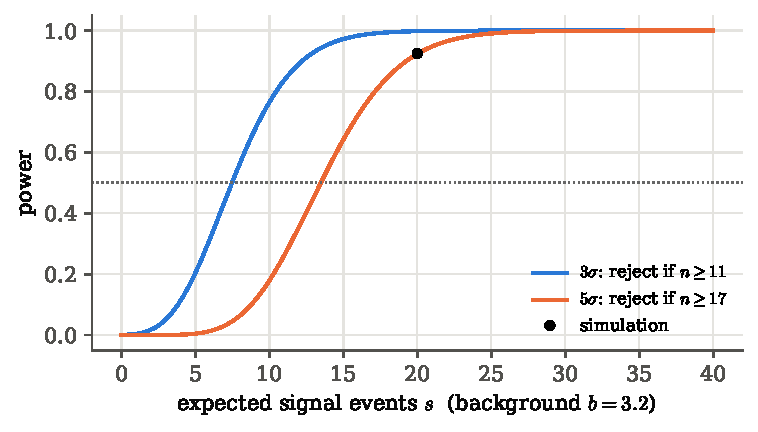
\includegraphics[width=0.8\linewidth]{figures/ch04/power_counting.pdf}
\caption{Power of a counting experiment with background $b=3.2$, for the
$3\sigma$ and the $5\sigma$ thresholds. Each curve rises from nearly zero to one
as the expected signal grows. The dotted line marks power one half, and the
black dot is a direct simulation at $s=20$.}
\label{4a:fig:power-counting}
\end{figure}

With discrete data a test usually has level $\alpha$ without having size
exactly $\alpha$: its false-alarm rate is below the target, and we call it
\emph{conservative}. The reason is that $N$ takes only integer values, so the
rejection probability under the null jumps as the cut moves from one integer
to the next. For example, the size of the test ``reject if $N\ge11$'' is
$\Prob(N\ge11\given b=3.2)=\FourACowanPone$, smaller than the $3\sigma$ target
$\FourAPzThreeOne$, and the next lower cut, $N\ge10$, would overshoot it.

\pyfile[firstline=72,lastline=87]{code/ch04/03_power_curves.py}{Critical count and power of a Poisson counting experiment}

The helper \pyname{n_crit} steps $n$ upward until the null tail
\pyname{stats.poisson.sf(n - 1, b)} drops below the threshold, which is
\eqref{4a:eq:power-poisson} read literally. The power curves are then the same
survival function with mean \pyname{b + s}. Nothing here needs an
approximation, which makes the counting experiment the best place to build
intuition about power before we meet statistics whose distributions must be
simulated.

\paragraph{Statistically significant is not the same as important.}
The power function of a consistent test climbs to one for \emph{every}
$\theta\in\Theta_1$ as $n\to\infty$, however close $\theta$ is to $\theta_0$.
With enough data, an effect too small to matter will be declared significant.
\mainref{p.~155} calls this the gap between statistical and scientific
significance: a rejection says the effect is probably not zero, not that it is
large. A confidence interval shows both at once, the distance from $\theta_0$
and the precision, and is often the more informative report. Every test can
be turned into a confidence interval, a construction taken up in the second
part of the chapter.
\section{The p-value is a random variable}
\label{4a:sec:uniform}

A p-value changes from one repetition of an experiment to the next. Imagine a
thousand groups, each running the same background-only experiment and each
computing a p-value. They will not get the same number. The data fluctuate, so
the test statistic fluctuates, so the p-value fluctuates
\srcref{Cowan}{p.~58}. The p-value is therefore a random variable with its own
distribution. That distribution is what gives ``reject if $p<\alpha$'' a known
false-alarm rate. It also shows, more clearly than any argument in words, why
a p-value is not the probability that the null is true.

\paragraph{The question in words.}
\begin{enumerate}[label=\arabic*.]
  \item How is the p-value related to the rejection regions of
        \cref{4a:sec:power}?
  \item If the null is true, how are p-values distributed? If it is false?
  \item In a collection of experiments where some nulls are true and some
        false, what fraction of the ``significant'' results are false alarms?
\end{enumerate}

\subsection{The smallest level at which we would reject}
\label{4a:sec:inf-alpha}

Suppose that for every $\alpha\in(0,1)$ we have a size-$\alpha$ test, with
rejection region $R_\alpha=\{T\ge c_\alpha\}$. A smaller $\alpha$ means a
stricter test, a larger $c_\alpha$ and a smaller region, so the regions are
nested. For our data, some of these tests reject and some do not, and there
is a smallest level at which the test still rejects. \mainref{Def.~10.11}
takes that as the definition,
\[
  p=\inf\bigl\{\alpha:\ T(\bm x)\in R_\alpha\bigr\},
\]
and \mainref{Thm~10.12} shows that it is the same tail probability as before.
For a simple null the argument is short. The observed value $t_{\rm obs}$ is on
the boundary of the region exactly when $c_\alpha=t_{\rm obs}$, and the size of
that region is $\Prob_{\theta_0}(T\ge t_{\rm obs})$. Any smaller $\alpha$ puts
the cut above $t_{\rm obs}$ and retains; any larger one rejects. So
\begin{equation}
  \text{reject at level }\alpha
  \quad\Longleftrightarrow\quad
  p\le\alpha .
  \label{4a:eq:p-le-alpha}
\end{equation}
This is why a p-value is more useful than a bare ``reject'': every reader can
apply their own $\alpha$. For a composite null the tail probability depends
on which $\theta\in\Theta_0$ is true, and the definition takes the worst case,
$p=\sup_{\theta\in\Theta_0}\Prob_\theta(T\ge t_{\rm obs})$, as we already did
for the coin in \cref{4a:sec:simple-composite}.

A widely used vocabulary for p-values \mainref{p.~157}:
\begin{center}
\begin{tabular}{ll}
\toprule
p-value & evidence against $\Hnull$ \\
\midrule
$<0.01$ & very strong \\
$0.01$--$0.05$ & strong \\
$0.05$--$0.10$ & weak \\
$>0.10$ & little or none \\
\bottomrule
\end{tabular}
\end{center}
Particle physicists would call $p=0.01$ an unremarkable fluctuation, for
reasons we come to in \cref{4a:sec:ztable}. The scale is a convention, and
conventions differ between fields.

\subsection{Under the null, p is uniform}
\label{4a:sec:p-uniform}

Let $T$ have a continuous distribution under $\Hnull$, with cumulative
distribution function $F_0(t)=\Prob_{\theta_0}(T\le t)$, increasing and
continuous. For an observed value $t$, the p-value is the upper tail,
$p=1-F_0(t)$. Now let the data be random, so that the p-value is the random
variable $P=1-F_0(T)$. For any $u\in(0,1)$,
\begin{align}
  \Prob_{\theta_0}(P\le u)
  &\eqby{1} \Prob_{\theta_0}\bigl(1-F_0(T)\le u\bigr) \notag\\
  &\eqby{2} \Prob_{\theta_0}\bigl(F_0(T)\ge1-u\bigr) \notag\\
  &\eqby{3} \Prob_{\theta_0}\bigl(T\ge F_0^{-1}(1-u)\bigr) \notag\\
  &\eqby{4} 1-F_0\bigl(F_0^{-1}(1-u)\bigr) \notag\\
  &\eqby{5} u .
  \label{4a:eq:p-uniform}
\end{align}
\begin{explain}
  \item Definition of $P$.
  \item Rearrange the inequality.
  \item $F_0$ is increasing, so applying $F_0^{-1}$ to both sides keeps the
        direction of the inequality.
  \item $\Prob(T\ge a)=1-F_0(a)$ for a continuous variable, since
        $\Prob(T=a)=0$.
  \item $F_0$ undoes $F_0^{-1}$.
\end{explain}
A variable with $\Prob(P\le u)=u$ for all $u$ is uniform on $(0,1)$
\mainref{Thm~10.14}. The fact behind it is the \newterm{probability integral
transform} \unpack{feeding a continuous random variable into its own CDF gives
a uniform variable}. Run backwards, the same fact turns uniform random numbers
into any distribution we like, by inversion (\cref{ch:06} uses it to
simulate). Put together with \eqref{4a:eq:p-le-alpha}, which says ``reject at
level $\alpha$'' is the same as ``$p\le\alpha$'', it gives a test whose
false-alarm probability is exactly $\alpha$. So when nothing is there, a
p-value is just a uniform random number. Values below $0.3$ occur $30\%$ of
the time and values below $0.03$ occur $3\%$ of the time: both are things that
happen, one ten times more often than the other.

When the alternative is true, the statistic tends to be larger, the tail beyond
it smaller, and the p-values pile up near zero. How strongly they pile up is
the power: by \eqref{4a:eq:p-le-alpha}, $\Prob_\theta(P\le\alpha)=\beta(\theta)$.

\paragraph{Example: p-values from Gaussian readings.}
Take $n=10$ readings of $\Normal(\mu,1)$ and the one-sided test of $\mu=0$,
with $p=1-\Phi(\sqrt{n}\,\bar x)$. The script
\pyname{code/ch04/04_pvalue_uniform.py} computes $200\,000$ such p-values for
each of three true means. The left panel of \cref{4a:fig:pvalue-hist} shows the
histograms. At $\mu=0$ the histogram is flat, a fraction $\FourAPUfracZero$ of
the p-values fall below $0.05$, and a Kolmogorov--Smirnov test of uniformity
(\cref{4a:sec:ks}) returns $p=\FourAPUks$, no evidence against flatness. At
$\mu=0.3$ a fraction $\FourAPUfracOne$ fall below $0.05$, and at $\mu=0.8$ a
fraction $\FourAPUfracTwo$: these are the powers of the test at those means.

\begin{figure}[htbp]
\centering
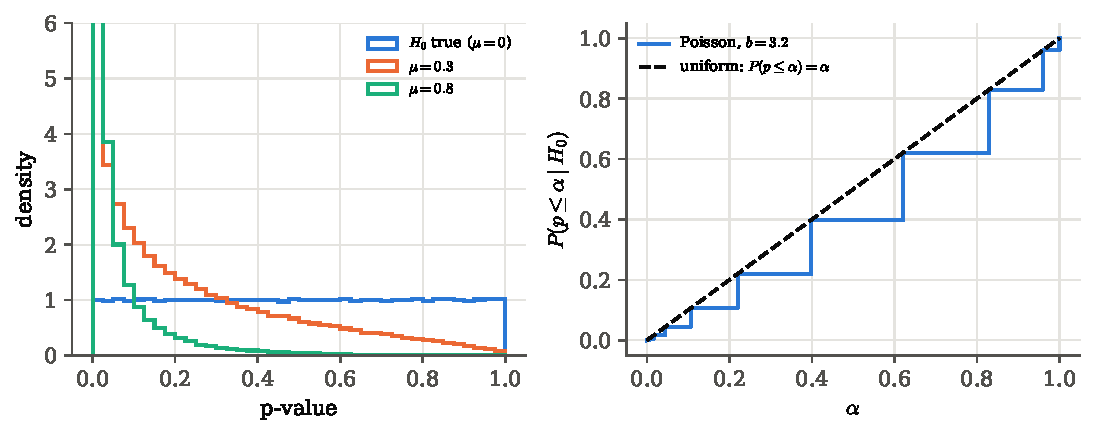
\includegraphics[width=\linewidth]{figures/ch04/pvalue_hist.pdf}
\caption{Left: histograms of p-values from many repetitions of the same
experiment. With the null true (blue) the histogram is flat; with a real effect
(orange, green) the p-values crowd towards zero, more so for the larger effect.
Right: for Poisson counts with $b=3.2$ the p-value takes only a few values, so
its cumulative distribution is a staircase. The staircase touches the diagonal
at its corners and otherwise stays below it, so ``reject if $p\le\alpha$'' never
rejects more often than $\alpha$.}
\label{4a:fig:pvalue-hist}
\end{figure}

\subsection{Discrete data: valid, not uniform}
\label{4a:sec:p-valid}

For a count the argument breaks at step (4) of \eqref{4a:eq:p-uniform},
because $\Prob(T=a)$ is no longer zero. The p-value can only take the values
$\pi(n)=\Prob_0(N\ge n)$ for integer $n$, so it cannot be uniform. What
survives is the inequality that matters for error control, the definition of
a \newterm{valid p-value} \unpack{one that is at most $\alpha$ with probability at
most $\alpha$ under the null, for every $\alpha$} \srcref{CasellaBerger}{Def.~8.3.26}:
\[
  \Prob_\theta(P\le u)\le u\qquad\text{for every }\theta\in\Theta_0\text{ and every }u\in[0,1].
\]
For a Poisson count the proof takes one line. The tail $\pi(n)$ decreases as
$n$ grows. Let $n_u$ be the smallest integer with $\pi(n_u)\le u$. Then
\begin{equation}
  \Prob_0(P\le u)
  \eqby{1} \Prob_0\bigl(\pi(N)\le u\bigr)
  \eqby{2} \Prob_0(N\ge n_u)
  \eqby{3} \pi(n_u)
  \relby{4}{\le} u .
  \label{4a:eq:p-valid}
\end{equation}
\begin{explain}
  \item The p-value of an observed count $N$ is $\pi(N)$.
  \item Because $\pi$ is decreasing, $\pi(N)\le u$ holds exactly when
        $N\ge n_u$.
  \item Definition of $\pi$.
  \item Definition of $n_u$.
\end{explain}
Equality holds only when $u$ happens to be one of the attainable values
$\pi(n)$, which are the corners of the staircase in the right panel of
\cref{4a:fig:pvalue-hist}. With $b=3.2$ the simulated fraction of null
experiments with $p\le0.05$ is $\FourAPUdisc$, below $0.05$. For a composite
null, the supremum over $\Theta_0$ in the definition of $p$ keeps it valid for
every member of the null \srcref{CasellaBerger}{Thm~8.3.27}.

\paragraph{A large p-value is not evidence for the null.}
A large $p$ can arise because $\Hnull$ is true, or because $\Hnull$ is false
and the test has too little power to notice \mainref{p.~157}. In the example
above, at $\mu=0.3$ three quarters of the p-values exceed $0.05$ although the
null is false. Failing to reject says ``these data cannot tell''. Testing is
built to find evidence \emph{against} a null, not to prove one
\mainref{p.~161}.

\subsection{What a p-value is not}
\label{4a:sec:not-posterior}

The most common misreading of a p-value is ``$p=0.04$, so there is a $4\%$
chance that the null is true''. \mainref{p.~157} and \srcref{Cowan}{p.~58} both
warn against it. The two numbers answer questions in opposite directions:
\[
  p=\Prob\bigl(\text{data this extreme or more}\given\Hnull\bigr)
  \qquad\text{versus}\qquad
  \Prob\bigl(\Hnull\given\text{data}\bigr).
\]
The first is a prediction from the null; the second is an inference about it.
Turning one into the other takes Bayes' theorem, and Bayes' theorem needs a
number the p-value never uses: how often the null is true before we look.
A simulation makes the difference concrete.

\paragraph{Example: a population of experiments.}
\emph{The setting.} Picture a field in which $90\%$ of the hypotheses people
test are really null, $\pi_0=0.9$. The other $10\%$ have an effect $\mu=0.5$
in the same experiment as above: $n=10$ Gaussian readings of unit variance,
tested one-sided against $\mu=0$. We simulate $10^6$ experiments, each picking
null or effect at random with these frequencies, and compute every p-value.

\emph{The question.} Among the ``significant'' experiments, those with
$p<0.05$, what fraction had a true null?

\emph{The two routes to a significant result.} A result can be significant
because the null is true and chance gave a small $p$, which happens with
probability $0.05$ by uniformity. Or it can be significant because there is an
effect and the test caught it, which happens with probability equal to the
power at $\mu=0.5$, $\FourAPUpower$.

\emph{Only then the numbers.} Weighting each route by how often it is taken,
Bayes' theorem gives
\begin{align}
  \Prob(\Hnull\given p<0.05)
  &\eqby{1} \frac{\Prob(p<0.05\given\Hnull)\,\pi_0}
                 {\Prob(p<0.05\given\Hnull)\,\pi_0+\Prob(p<0.05\given\Halt)\,(1-\pi_0)} \notag\\
  &\eqby{2} \frac{0.05\times0.9}{0.05\times0.9+\FourAPUpower\times0.1}
   \approx \FourAPUnullSigTh .
  \label{4a:eq:false-discovery}
\end{align}
\begin{explain}
  \item Bayes' theorem with the two hypotheses as the branches of a
        probability tree: first choose null or effect, then the p-value.
  \item Under the null $P$ is uniform, so $\Prob(P<0.05)=0.05$; under the
        effect it is the power.
\end{explain}
Almost half of the significant results are false alarms; the simulation
counts a fraction $\FourAPUnullSig$. Now narrow the selection to results that
only just made it, $0.04<p<0.05$. Under the null this band has probability
$0.01$ (uniformity again), and under the effect it has a probability we
compute from \eqref{4a:eq:power-z}. The same formula gives
$\FourAPUnullBandTh$, and the simulation $\FourAPUnullBand$: two thirds of the
barely significant results come from true nulls, while each of them reports
``$p<0.05$''. \Cref{4a:fig:pvalue-population} shows why: the flat carpet of null
p-values is ten times more populous than the effect experiments, and near
$p=0.05$ the carpet dominates.

\begin{figure}[htbp]
\centering
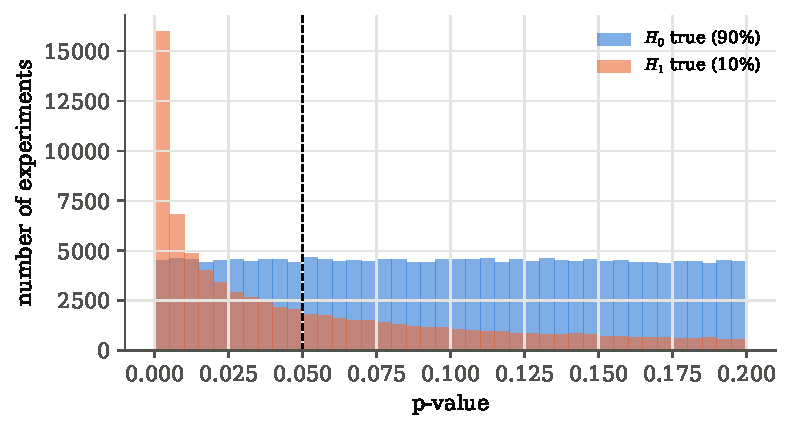
\includegraphics[width=0.8\linewidth]{figures/ch04/pvalue_population.pdf}
\caption{p-values from a population of experiments in which $90\%$ of the nulls
are true. The blue histogram (true nulls) is flat; the orange one (real
effects) rises towards zero. Left of the dashed line at $p=0.05$ both
contribute, and just left of it the flat blue carpet is the larger.}
\label{4a:fig:pvalue-population}
\end{figure}

\pyfile[firstline=61,lastline=78]{code/ch04/04_pvalue_uniform.py}{A population of experiments: how many significant results are false alarms?}

The code draws one Boolean per experiment, \pyname{is_null}, with probability
$\pi_0$, and sets the true mean to $0$ or $0.5$ accordingly. It draws the
sample mean directly from $\Normal(\mu,\sigma^2/n)$, which is its exact
distribution, converts it to a p-value, and then simply counts: among the
experiments with \pyname{pp < 0.05}, what fraction have \pyname{is_null}?
The analytic lines below are \eqref{4a:eq:false-discovery} and its narrow-band
version.

\begin{pitfall}[$p$ is not $\Prob(\Hnull\given\text{data})$]
The p-value is computed assuming the null is true, so it cannot be the
probability that the null is true. The fraction of significant results that
are false alarms depends on the power and on how often nulls are true in the
first place, neither of which enters $p$. In the example, $p<0.05$ went with a
$\FourAPUnullSig$ chance of a true null, and $0.04<p<0.05$ with a
$\FourAPUnullBand$ chance. The inference direction is the subject of
\cref{ch:05}.
\end{pitfall}

This does not make p-values useless. It makes them one ingredient. A small
p-value says the data are hard to produce by chance alone; whether that makes
the alternative probable depends on how plausible it was to begin with. That
is the logic behind the $5\sigma$ convention of \cref{4a:sec:ztable}, and it
is exactly the prior-times-likelihood structure of Bayes' theorem.
\section{Three workhorse tests: Wald, Student's t and permutation}
\label{4a:sec:wald}

A calorimeter is calibrated twice, a week apart, on the $661.7\,$keV gamma
line of $^{137}$Cs. The first run records $12$ reconstructed peak positions,
the second $15$. The second run's mean is higher. Did the energy
scale drift, or is this the scatter we expect from a detector with a
resolution of a few keV? Situations like this, comparing two samples or
comparing an estimate with a reference value, are the everyday business of
testing. Most tests for them are one of three kinds.
\begin{enumerate}[label=\arabic*.]
  \item The \emph{Wald test}: divide the estimate's distance from the null
        value by its estimated standard error and compare with a normal
        distribution. It works for any estimator that is approximately normal.
  \item The \emph{t-test}: the same ratio, with the exact distribution that
        accounts for having estimated the standard error from few Gaussian
        readings.
  \item The \emph{permutation test}: no distributional assumption at all; the
        null distribution is built by shuffling the labels of the data.
\end{enumerate}
Most powerful tests in the sense of \cref{4a:sec:np} often do not exist for
composite hypotheses, so these general-purpose tests carry most of the load
\mainref{p.~152}.

\subsection{The Wald test}
\label{4a:sec:wald-test}

Let $\hat\theta$ be an estimate of a scalar parameter $\theta$ with estimated
standard error $\widehat{\rm se}$, and suppose $\hat\theta$ is approximately
normal, as maximum-likelihood estimators are for large samples
(\cref{ch:03}). To test $\Hnull:\theta=\theta_0$ against
$\Halt:\theta\neq\theta_0$ we measure the distance in standard errors,
\begin{equation}
  W=\frac{\hat\theta-\theta_0}{\widehat{\rm se}},
  \qquad
  \text{reject }\Hnull\text{ when }\abs{W}>z_{\alpha/2}
  \label{4a:eq:wald}
\end{equation}
\mainref{Def.~10.3}. Under the null, $W$ is approximately standard normal, so
\begin{equation}
  \Prob_{\theta_0}\bigl(\abs{W}>z_{\alpha/2}\bigr)\;\longrightarrow\;\Prob\bigl(\abs{Z}>z_{\alpha/2}\bigr)=\alpha
  \qquad(n\to\infty),
  \label{4a:eq:wald-size}
\end{equation}
which is \mainref{Thm~10.4}: the Wald test has size $\alpha$ asymptotically.
The p-value of an observed $w$ is the two-sided normal tail
\mainref{(10.7)}:
\begin{equation}
  p=\Prob_{\theta_0}\bigl(\abs{W}>\abs{w}\bigr)\approx\Prob\bigl(\abs{Z}>\abs{w}\bigr)=2\Phi(-\abs{w}).
  \label{4a:eq:wald-p}
\end{equation}
The standard error may also be computed at the null value, ${\rm se}_0$, in
place of the estimate; both versions are valid \mainref{Remark~10.5}. For a
binomial proportion $\hat p$ tested against $p_0$, for instance, one may use
${\rm se}_0=\sqrt{p_0(1-p_0)/n}$, which needs no estimate at all.

\paragraph{Example: comparing two means.}
Two independent samples $X_1,\dots,X_m$ and $Y_1,\dots,Y_n$ have means
$\mu_1,\mu_2$. The null is $\delta=\mu_1-\mu_2=0$, the estimate is
$\hat\delta=\bar X-\bar Y$, and because the samples are independent the
variances add \mainref{Ex.~10.8}:
\begin{equation}
  \widehat{\rm se}=\sqrt{\frac{s_1^2}{m}+\frac{s_2^2}{n}},
  \qquad
  W=\frac{\bar X-\bar Y}{\sqrt{s_1^2/m+s_2^2/n}},
  \label{4a:eq:two-means}
\end{equation}
with $s_1^2,s_2^2$ the two sample variances. In Wasserman's cholesterol data
\mainref{Ex.~10.15} the two group means are $216.2$ and $195.3$ with standard
errors $5$ and $2.4$, so
$W=(216.2-195.3)/\sqrt{5^2+2.4^2}=20.9/5.55\approx3.78$ and
$p=2\Phi(-3.78)=\FourACholP$, the quoted $0.0002$. The same recipe works for
medians, with the standard error of the difference of sample medians taken
from the bootstrap of \cref{ch:03} \mainref{Ex.~10.9}; there $W=2.4$ and
$p=0.02$.

\paragraph{Example: two classifiers, and paired data.}
\mainref{Ex.~10.7} compares two prediction algorithms, and the same logic
compares two event classifiers. If each is run on its own test set, of sizes
$m$ and $n$, the error counts are independent binomials and
\eqref{4a:eq:two-means} applies with $s_i^2=\hat p_i(1-\hat p_i)$. If both run
on the \emph{same} test set, the two error rates are correlated and the
variances no longer add. The fix is to test the per-event difference: let
$X_i=1$ if the first classifier is right on event $i$, $Y_i$ likewise for the
second, and $D_i=X_i-Y_i$. Then $\hat\delta=\bar D$, $\widehat{\rm se}=S_D/\sqrt n$
with $S_D$ the sample standard deviation of the $D_i$, and $W=\bar D/\widehat{\rm se}$.
This \newterm{paired comparison} removes the event-to-event variation that both
classifiers share, which is usually most of it.

\subsection{Small samples: Student's t}
\label{4a:sec:t-test}

The Wald test's guarantee is asymptotic. With few readings, the estimated
standard error is itself noisy, and a too-small $\widehat{\rm se}$ inflates
$\abs{W}$. We can see how badly by simulation: draw $n$ readings from
$\Normal(0,1)$, so the null $\mu=0$ is true, compute
$T=\sqrt n\,\bar X/S$ with $S$ the sample standard deviation, and count how
often $\abs T>1.96$. \Cref{4a:fig:wald-size} shows the answer: the false-alarm
rate is $\FourAWaldSizeThree$ at $n=3$, $\FourAWaldSizeFive$ at $n=5$,
$\FourAWaldSizeTen$ at $n=10$ and $\FourAWaldSizeThirty$ at $n=30$, instead of
$0.05$.

For Gaussian data the exact distribution of $T$ is known. Write
\begin{align}
  T=\frac{\sqrt n(\bar X-\mu_0)}{S}
  &\eqby{1} \frac{\sqrt n(\bar X-\mu_0)/\sigma}{S/\sigma} \notag\\
  &\eqby{2} \frac{Z}{\sqrt{V/(n-1)}},
  \qquad Z\sim\Normal(0,1),\quad V=\frac{(n-1)S^2}{\sigma^2}\sim\chi^2_{n-1} .
  \label{4a:eq:t-stat}
\end{align}
\begin{explain}
  \item Divide numerator and denominator by the unknown $\sigma$; the ratio is
        unchanged, so $T$ does not depend on $\sigma$.
  \item Under the null the numerator is standard normal. In the denominator,
        $S/\sigma=\sqrt{V/(n-1)}$, and $(n-1)S^2/\sigma^2$ is $\chi^2_{n-1}$ and
        independent of $\bar X$ for Gaussian data (\cref{ch:03}).
\end{explain}
A standard normal divided by the square root of an independent
$\chi^2_k/k$ is by definition a \newterm{Student t variable} with $k$ degrees
of freedom \unpack{a bell curve with heavier tails, because the denominator
sometimes comes out small}, with density \mainref{p.~170}
\begin{equation}
  f(t)=\frac{\Gamma\bigl(\tfrac{k+1}{2}\bigr)}{\sqrt{k\pi}\,\Gamma\bigl(\tfrac k2\bigr)}
       \Bigl(1+\frac{t^2}{k}\Bigr)^{-(k+1)/2} .
  \label{4a:eq:t-density}
\end{equation}
For $k=1$ it is the Cauchy distribution of \cref{ch:02}, and as
$k\to\infty$ it becomes the standard normal, because
$(1+t^2/k)^{-(k+1)/2}\to e^{-t^2/2}$ and $V/k\to1$ by the law of large numbers.
So $T\sim t_{n-1}$ exactly, and the \newterm{t-test} rejects when
$\abs T>t_{n-1,\alpha/2}$, the upper $\alpha/2$ quantile of $t_{n-1}$. The same
fact lets us compute, not just simulate, how often the Wald test rejects a
true null. The Wald test uses the normal cut $1.96$, so its size is
$\Prob(\abs{t_{n-1}}>1.96)$, which for $n=3$ is $\FourAWaldSizeThreeEx$, the
solid line in \cref{4a:fig:wald-size}. The t-test's simulated size is
$\FourATSizeThree$ at $n=3$ and $\FourATSizeTen$ at $n=10$. For moderately
large $n$ the two tests are the same test.

\begin{figure}[htbp]
\centering
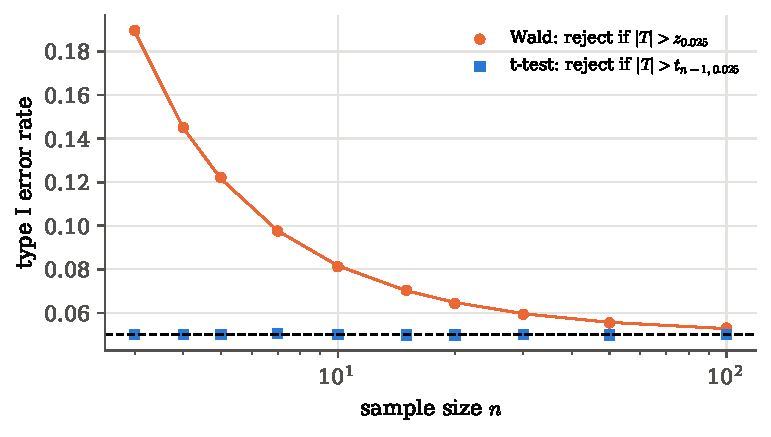
\includegraphics[width=0.8\linewidth]{figures/ch04/wald_size.pdf}
\caption{How often a test rejects a true null, as a function of the number of
Gaussian readings. The Wald test, which uses the normal cut $1.96$ with an
estimated standard error, rejects too often for small samples (orange dots,
with the exact curve as a line). The t-test, which uses the t quantile,
stays on the dashed $0.05$ line at every sample size (blue squares).}
\label{4a:fig:wald-size}
\end{figure}

For two samples with possibly different variances, the ratio
\eqref{4a:eq:two-means} is not exactly t-distributed. \newterm{Welch's t-test}
uses a t distribution with an effective number of degrees of freedom computed
from $s_1,s_2,m,n$; it is what \pyname{scipy.stats.ttest_ind(..., equal_var=False)}
does.

\subsection{The permutation test}
\label{4a:sec:permutation}

The t-test is exact only for Gaussian data. The \newterm{permutation test}
is exact for any distribution, at the price of a computation
\mainref{\S10.5}. The null it tests is that the two samples come from the
same distribution, $\Hnull:F_X=F_Y$. The key observation: if that is true, the
labels ``first sample'' and ``second sample'' carry no information. Every way
of splitting the pooled $N=m+n$ values into a group of $m$ and a group of $n$
was equally likely to have produced the data we saw. So we can build the null
distribution of any statistic $T$ by recomputing it for all $N!$ orderings of
the pooled values, each with probability $1/N!$. That is the
\newterm{permutation distribution}, and the p-value is the fraction of
orderings with $T$ larger than the observed value.

\paragraph{Example: the smallest possible permutation test.}
Take $(X_1,X_2,Y_1)=(1,9,3)$ and $T=\abs{\bar X-\bar Y}$
\mainref{Ex.~10.19}. The observed value is $\abs{(1+9)/2-3}=2$. The six
orderings, with the first two entries playing the role of $X$:
\begin{center}
\begin{tabular}{ccc}
\toprule
ordering & $T$ & probability \\
\midrule
$(1,9,3)$, $(9,1,3)$ & $\abs{5-3}=2$ & $2/6$ \\
$(1,3,9)$, $(3,1,9)$ & $\abs{2-9}=7$ & $2/6$ \\
$(3,9,1)$, $(9,3,1)$ & $\abs{6-1}=5$ & $2/6$ \\
\bottomrule
\end{tabular}
\end{center}
Four of the six give $T>2$, so $p=\Prob_0(T>2)=4/6=\FourAToyP$. The script
enumerates the six orderings with \pyname{itertools.permutations} and gets the
same number. (Some authors count $T\ge t_{\rm obs}$, which includes the
observed ordering itself; with continuous data and many orderings the
difference is negligible.)

For real data $N!$ is astronomically large, so we sample orderings at random.
The algorithm \mainref{p.~163} is:
\begin{enumerate}[label=\arabic*.]
  \item compute $t_{\rm obs}$ from the data as labelled;
  \item shuffle the pooled data, split into groups of $m$ and $n$, and
        recompute $T$;
  \item repeat step 2 $B$ times, giving $T_1,\dots,T_B$;
  \item the p-value is approximately $\frac1B\sum_{j=1}^B I(T_j>t_{\rm obs})$,
        with $I$ the indicator (one if true, zero if false).
\end{enumerate}
Why is this legitimate? Under the null the $N$ values are exchangeable: their
joint distribution does not change when we reorder them. Given the set of
values that occurred, every assignment of labels is equally likely, so the
shuffled statistics are draws from the exact conditional null distribution of
$T$. No normality, no large-sample limit, no estimate of a standard error is
involved. The permutation test is most useful when there are few samples and
the statistic has no convenient formula for its distribution. Wasserman's
gene-expression example is of this kind (\mainref{Ex.~10.20}: ten patients,
two tumour types, $T$ the absolute difference of medians $=710$,
$p=0.045$).

\paragraph{Example: the calorimeter calibration.}
Back to the two calibration runs. We simulate run 1 as $12$ readings
from $\Normal(661.7,4^2)\,$keV and run 2 as $15$ readings with a true shift of
$3.3\,$keV (script \pyname{05_wald_t_permutation.py}). The observed means are $\FourACalMeanOne$ and $\FourACalMeanTwo\,$keV
with sample standard deviations $\FourACalSdOne$ and $\FourACalSdTwo\,$keV.
By \eqref{4a:eq:two-means},
\begin{align*}
  \hat\delta &= \FourACalMeanTwo-\FourACalMeanOne=\FourACalD\ \text{keV},\\
  \widehat{\rm se} &= \sqrt{\FourACalSdOne^2/12+\FourACalSdTwo^2/15}=\FourACalSe\ \text{keV},\\
  W &= \FourACalD/\FourACalSe=\FourACalW ,
\end{align*}
so the Wald p-value is $2\Phi(-\FourACalW)=\FourACalPwald$. Welch's t-test gives
$\FourACalPwelch$, larger because it accounts for the uncertainty in the two
standard deviations. The permutation test, with $B=100\,000$ shuffles of the
$27$ values, gives $\FourACalPperm$. \Cref{4a:fig:permutation} shows the
permutation distribution of $\bar x_2-\bar x_1$ with the observed difference
marked. The three p-values are close to one another: they ask the same question
in three ways. None of them would convince a particle physicist of a new effect.
Nor could they be expected to. With twelve and fifteen readings of $4\,$keV
resolution, the true shift of $3.3\,$keV is only
$3.3/\sqrt{4^2/12+4^2/15}\approx2.1$ standard errors on average, and a single pair
of runs can easily show much less or much more. This experiment is too small to
find the shift reliably.

\begin{figure}[htbp]
\centering
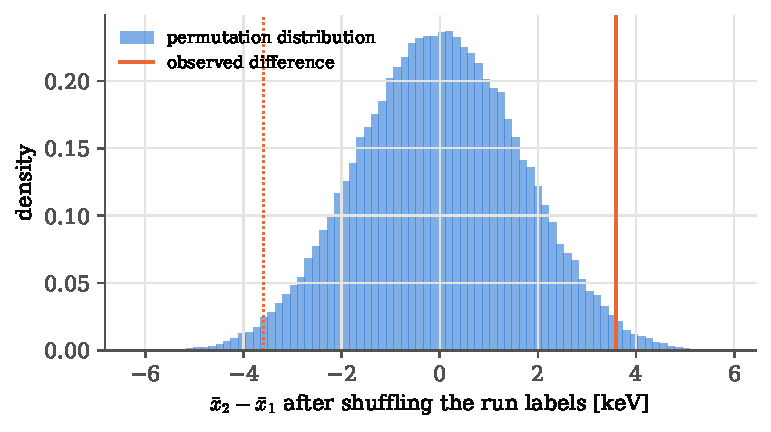
\includegraphics[width=0.8\linewidth]{figures/ch04/permutation_dist.pdf}
\caption{The permutation distribution for the calibration example: the
difference of the two run means after randomly reassigning the $27$ readings
to the two runs, $100\,000$ times. The solid orange line is the observed
difference and the dotted one its mirror image; the fraction of shuffles
beyond either line is the two-sided p-value.}
\label{4a:fig:permutation}
\end{figure}

\pyfile[firstline=48,lastline=66]{code/ch04/05_wald_t_permutation.py}{Wald, Welch and permutation tests for two calibration runs}

The loop is the algorithm above, line for line: \pyname{rng.permutation}
shuffles the pooled readings, the first $m$ play run 1 and the rest run 2,
and the difference of means is stored. The p-value counts shuffles with
$\abs{T_j}\ge\abs{t_{\rm obs}}$ (two-sided). As a cross-check the script calls
\pyname{scipy.stats.permutation_test} with $20\,000$ resamples, which returns
$\FourACalPpermScipy$. Both numbers are Monte Carlo estimates, so they carry a
random error. For the shorter run of $20\,000$ resamples that error is
$\sqrt{p(1-p)/20\,000}$, a few thousandths at most. The two estimates differ by
$\FourACalPermDiffSig$ times their combined error; more shuffles would bring them together. In large samples the permutation test
usually agrees with the asymptotic tests, and it is most valuable for small
samples \mainref{p.~164}.

\paragraph{Tests and intervals are two views of one object.}
There is a simple link between the Wald test and the familiar interval
$\hat\theta\pm z_{\alpha/2}\widehat{\rm se}$. By \eqref{4a:eq:wald},
$\abs{\hat\theta-\theta_0}>z_{\alpha/2}\widehat{\rm se}$ says precisely that
$\theta_0$ lies outside that interval. So the size-$\alpha$ Wald test rejects
$\theta_0$ if and only if $\theta_0$ is outside the $1-\alpha$ interval
\mainref{Thm~10.10}. The second part of the chapter turns that observation
into a general machine for building confidence intervals from tests.
\section{The best test: the Neyman--Pearson lemma}
\label{4a:sec:np}

A trigger has to decide, event by event, whether a collision looks like
signal or like background. Each event comes with several measured
quantities: energies, angles, isolation variables. Any selection keeps some
signal and some background. At a fixed signal efficiency, say $90\%$, one
selection keeps less background than another, and we would like the best one.
Put as a question about tests: among all tests
with the same size $\alpha$, which has the largest power? For two simple
hypotheses there is a complete answer, and it is one of the few genuinely
optimal results in statistics.

\paragraph{The question in words.}
\begin{enumerate}[label=\arabic*.]
  \item We have a fixed budget $\alpha$ of false-alarm probability. Which
        outcomes should we spend it on?
  \item Does the answer depend on the particular alternative, or is one test
        best against a whole family of alternatives?
  \item What do we do when the densities are only available as simulated
        events in many dimensions?
\end{enumerate}

\subsection{Spending a false-alarm budget}
\label{4a:sec:np-budget}

Take a simple null and a simple alternative, $\Hnull:\theta=\theta_0$ versus
$\Halt:\theta=\theta_1$, with densities $f_0(\bm x)=f(\bm x\given\theta_0)$ and
$f_1(\bm x)=f(\bm x\given\theta_1)$ for the whole data set. A test is a choice
of rejection region $R$. Its size and power are
\[
  \alpha=\int_R f_0(\bm x)\,\dd\bm x,
  \qquad
  \beta(\theta_1)=\int_R f_1(\bm x)\,\dd\bm x .
\]
Think of each small cell $\dd\bm x$ of data space as an item we can put into
$R$. It costs $f_0\,\dd\bm x$ of the false-alarm budget and buys $f_1\,\dd\bm x$
of power. The budget is fixed. To buy as much power as possible we should take
the items with the best value for money first, the cells where the ratio
$f_1/f_0$ is largest, and keep taking them in order of decreasing ratio until
the budget is spent. The region we end up with is
$R=\{\bm x:\ f_1(\bm x)/f_0(\bm x)>k\}$, with the threshold $k$ fixed by the
budget.

The same answer comes out of the Lagrange-multiplier method familiar from
mechanics. We maximise $\int_Rf_1$ subject to $\int_Rf_0=\alpha$, so we
maximise $\int_R(f_1-kf_0)\,\dd\bm x$ for a multiplier $k$. The integrand can
be positive or negative, and the integral over $R$ is largest when $R$
contains every point where $f_1-kf_0>0$ and no point where it is negative.
The multiplier is the exchange rate between power and size.

\begin{keyidea}[Neyman--Pearson lemma]
For testing a simple $\Hnull:\theta=\theta_0$ against a simple
$\Halt:\theta=\theta_1$, the test that rejects when the
\newterm{likelihood ratio}
\[
  \Lambda(\bm x)=\frac{f(\bm x\given\theta_1)}{f(\bm x\given\theta_0)}
  =\frac{\Like(\theta_1)}{\Like(\theta_0)}
\]
exceeds a constant $k$, with $k$ chosen so that
$\Prob_{\theta_0}(\Lambda>k)=\alpha$, has the largest power of all tests of
level $\alpha$ \mainref{Thm~10.30}, \srcref{CasellaBerger}{Thm~8.3.12},
\srcref{Cowan}{(4.12)}. The ratio collapses any number of measured variables
into one number, and no other function of the data does better.
\end{keyidea}

\paragraph{Why it is true.}
The budget argument is the proof in disguise. To make it exact, describe a
test by its \newterm{test function} $\phi(\bm x)$ \unpack{one where the test
rejects, zero where it retains}, so that size and power are $\int\phi f_0$ and
$\int\phi f_1$. Let $\phi$ be the likelihood-ratio test and $\phi'$ any other
test of level $\alpha$, with power functions $\beta$ and $\beta'$. At every
point, $[\phi(\bm x)-\phi'(\bm x)][f_1(\bm x)-kf_0(\bm x)]\ge0$: where
$f_1>kf_0$ we have $\phi=1\ge\phi'$, and where $f_1<kf_0$ we have
$\phi=0\le\phi'$, so the two factors never have opposite signs. Integrating,
\begin{align}
  0 &\relby{1}{\le} \int\bigl[\phi(\bm x)-\phi'(\bm x)\bigr]\bigl[f_1(\bm x)-kf_0(\bm x)\bigr]\dd\bm x \notag\\
    &\eqby{2} \bigl[\beta(\theta_1)-\beta'(\theta_1)\bigr]-k\bigl[\beta(\theta_0)-\beta'(\theta_0)\bigr] \notag\\
    &\relby{3}{\le} \beta(\theta_1)-\beta'(\theta_1) .
  \label{4a:eq:np-proof}
\end{align}
\begin{explain}
  \item The integrand is non-negative at every point, as just argued.
  \item Multiply out: $\int\phi f_1=\beta(\theta_1)$, $\int\phi f_0=\beta(\theta_0)$,
        and likewise for $\phi'$.
  \item $\beta(\theta_0)=\alpha$ for the likelihood-ratio test, and
        $\beta'(\theta_0)\le\alpha$ because $\phi'$ has level $\alpha$; so the
        bracket multiplying $k\ge0$ is non-negative, and dropping it can only
        increase the right-hand side.
\end{explain}
So $\beta(\theta_1)\ge\beta'(\theta_1)$: no level-$\alpha$ test beats the
likelihood ratio \srcref{CasellaBerger}{p.~315}. For discrete data replace
integrals by sums. Notice what the proof used: nothing about the shape of the
densities, the dimension of $\bm x$, or large samples. The lemma is exact.

\paragraph{Example: the Gaussian mean, and a uniformly best test.}
Let $X_1,\dots,X_n\iid\Normal(\mu,\sigma^2)$, $\sigma$ known, and test
$\mu=0$ against a single $\mu=\mu_1>0$. The log of the likelihood ratio is
\begin{align}
  \ln\Lambda
  &\eqby{1} \sum_{i=1}^n\Bigl[-\frac{(x_i-\mu_1)^2}{2\sigma^2}+\frac{x_i^2}{2\sigma^2}\Bigr] \notag\\
  &\eqby{2} \sum_{i=1}^n\frac{2\mu_1x_i-\mu_1^2}{2\sigma^2}
   \eqby{3} \frac{n\mu_1}{\sigma^2}\,\bar x-\frac{n\mu_1^2}{2\sigma^2} .
  \label{4a:eq:np-gauss}
\end{align}
\begin{explain}
  \item The likelihood is a product of Gaussians; its log is a sum. The
        normalisations $1/\sqrt{2\pi\sigma^2}$ are the same under both
        hypotheses and cancel.
  \item Expand $(x_i-\mu_1)^2=x_i^2-2\mu_1x_i+\mu_1^2$; the $x_i^2$ terms
        cancel.
  \item $\sum_ix_i=n\bar x$.
\end{explain}
Because $\mu_1>0$, $\ln\Lambda$ increases with $\bar x$, so ``$\Lambda>k$''
is the same event as ``$\bar x>c$'' for some $c$. The most powerful test is
the one-sided test of \cref{4a:sec:power-function}, with
$c=\sigma z_\alpha/\sqrt n$ to give size $\alpha$ \srcref{CasellaBerger}{Ex.~8.3.15}.

The value of $\mu_1$ has disappeared from the rejection region. Neither the
event $\bar x>c$ nor the cut $c=\sigma z_\alpha/\sqrt n$ mentions it. So the
same region is most powerful against \emph{every} $\mu_1>0$. A test with this
property is \newterm{uniformly most powerful}. Such tests exist
when the likelihood ratio is monotone in one statistic, as for one-sided
problems in exponential families. For two-sided alternatives they usually do
not: the best test against $\mu_1>0$ rejects for large $\bar x$, the best
against $\mu_1<0$ rejects for small $\bar x$, and no single region is best
against both \mainref{p.~152}.

\paragraph{Example: discreteness restricts the available sizes.}
Let $X\sim\mathrm{Binomial}(2,\theta)$, testing $\theta=\frac12$ against
$\theta=\frac34$ \srcref{CasellaBerger}{Ex.~8.3.14}. The pmfs are
$\binom2x\theta^x(1-\theta)^{2-x}$, giving
$(\frac14,\frac12,\frac14)$ and $(\frac1{16},\frac6{16},\frac9{16})$ for
$x=0,1,2$, so the ratios are
\[
  \Lambda(0)=\frac{1/16}{1/4}=\frac14,\qquad
  \Lambda(1)=\frac{6/16}{1/2}=\frac34,\qquad
  \Lambda(2)=\frac{9/16}{1/4}=\frac94 .
\]
Ranking the outcomes by $\Lambda$ and filling the budget: rejecting on
$\{2\}$ is the most powerful test of size $\Prob_{1/2}(X=2)=\frac14$; rejecting
on $\{1,2\}$ is the most powerful test of size $\frac34$. No non-randomised
test has size $0.05$ except the one that never rejects. With discrete data the
lemma still says what to do, but only certain sizes can be achieved, as we saw
for the Poisson counts in \cref{4a:sec:power-counting}.

\subsection{Selecting particles: efficiency, purity and the ratio}
\label{4a:sec:selection}

Selecting events is a test, and the lemma tells us how to do it best.
\srcref{Cowan}{\S4.2} takes a charged
particle of known momentum whose ionisation $t$ is measured. Electrons and
pions deposit different amounts on average, so $t$ has density $g(t\given e)$
for electrons and $g(t\given\pi)$ for pions. Selecting electron candidates with
a cut $t<t_{\rm cut}$ defines two efficiencies \srcref{Cowan}{(4.3)--(4.4)},
\[
  \varepsilon_e=\int_{-\infty}^{t_{\rm cut}}g(t\given e)\,\dd t=1-\alpha,
  \qquad
  \varepsilon_\pi=\int_{-\infty}^{t_{\rm cut}}g(t\given\pi)\,\dd t=\beta_{\rm II} .
\]
Here the \emph{signal} plays the role of the null: rejecting ``it is an
electron'' when it is one loses signal, with probability $\alpha$, and keeping
a pion is a type II error. The purity of the selected sample follows from
Bayes' theorem with the particle fractions $a_e$ and $a_\pi=1-a_e$ as prior
probabilities \srcref{Cowan}{(4.8)--(4.11)}:
\begin{equation}
  P_e=\frac{\text{electrons kept}}{\text{particles kept}}
  =\frac{a_e\,\varepsilon_e}{a_e\,\varepsilon_e+a_\pi\,\varepsilon_\pi} .
  \label{4a:eq:purity}
\end{equation}
This is the same structure as \eqref{4a:eq:false-discovery}: the purity of a
selection, like the fraction of true discoveries, needs the prior fractions.
At fixed efficiency $\varepsilon_e$ the purity is largest when
$\varepsilon_\pi$ is smallest, which is the Neyman--Pearson problem. With one
variable and a monotone ratio a single cut is automatically optimal. With a
vector of variables $\bm x$ the lemma says to keep the events with
$g(\bm x\given e)/g(\bm x\given\pi)>c$ \srcref{Cowan}{(4.12)--(4.13)}.

In practice $g(\bm x\given H)$ is known only through simulated events. With
$M$ histogram bins per variable and $n$ variables there are $M^n$ bins to fill,
which becomes impossible beyond a few variables \srcref{Cowan}{p.~51}. One
retreat is a linear statistic $t=\bm a\T\bm x$. Fisher chose the direction
$\bm a$ that maximises the separation of the two class means relative to the
spread within the classes, $(\tau_0-\tau_1)^2/(\Sigma_0^2+\Sigma_1^2)$, and
found \srcref{Cowan}{(4.23)}
\begin{equation}
  \bm a\propto\bm W^{-1}(\bm\mu_0-\bm\mu_1),\qquad\bm W=\bm V_0+\bm V_1,
  \label{4a:eq:fisher-disc}
\end{equation}
with $\bm\mu_k$ and $\bm V_k$ the mean vector and covariance matrix of $\bm x$
under hypothesis $k$. When both classes are Gaussian with the \emph{same}
covariance $\bm V$, Fisher's discriminant is exactly the log likelihood ratio.
Writing $Q_k=(\bm x-\bm\mu_k)\T\bm V^{-1}(\bm x-\bm\mu_k)$ for the quadratic
form in each Gaussian exponent,
\begin{align}
  \ln\frac{\Normal(\bm x;\bm\mu_0,\bm V)}{\Normal(\bm x;\bm\mu_1,\bm V)}
  &\eqby{1} -\tfrac12Q_0+\tfrac12Q_1 \notag\\
  &\eqby{2} (\bm\mu_0-\bm\mu_1)\T\bm V^{-1}\bm x
       -\tfrac12\bigl(\bm\mu_0\T\bm V^{-1}\bm\mu_0-\bm\mu_1\T\bm V^{-1}\bm\mu_1\bigr) .
  \label{4a:eq:fisher-lr}
\end{align}
\begin{explain}
  \item The normalisations $(2\pi)^{-n/2}\det\bm V^{-1/2}$ are equal and cancel.
  \item Expand $Q_k=\bm x\T\bm V^{-1}\bm x-2\bm\mu_k\T\bm V^{-1}\bm x+\bm\mu_k\T\bm V^{-1}\bm\mu_k$
        (using the symmetry of $\bm V^{-1}$). The quadratic term in $\bm x$ is
        the same for both and cancels, leaving a linear function of $\bm x$.
\end{explain}
The coefficient vector is $\bm V^{-1}(\bm\mu_0-\bm\mu_1)$, proportional to
Fisher's with $\bm W=2\bm V$ \srcref{Cowan}{(4.27)--(4.28)}. When the covariances
differ, the $\bm x\T\bm V_k^{-1}\bm x$ terms no longer cancel, the optimal
boundary is curved, and a linear statistic loses power. Nonlinear methods,
neural networks and boosted trees, are in this light approximations to the
likelihood ratio learned from simulated events \srcref{Cowan}{\S4.4.2}: a
classifier trained to separate two classes outputs, at best, a monotone
function of $g(\bm x\given H_0)/g(\bm x\given H_1)$.

\paragraph{Example: three selections, and three hundred random ones.}
We make signal and background Gaussian in two variables
(script \pyname{06_neyman_pearson.py}), with different means and different covariance
matrices, and compare three selections at a signal efficiency of $90\%$: a
cut on $x_1$ alone, Fisher's linear discriminant \eqref{4a:eq:fisher-disc}
trained on $20\,000$ events of each class, and the exact log likelihood ratio.
\Cref{4a:fig:np-scatter} shows the events and the three decision boundaries.
The fractions of background kept are $\FourANPbkgCut$ for the $x_1$ cut,
$\FourANPbkgFisher$ for Fisher and $\FourANPbkgLR$ for the likelihood ratio.

\begin{figure}[htbp]
\centering
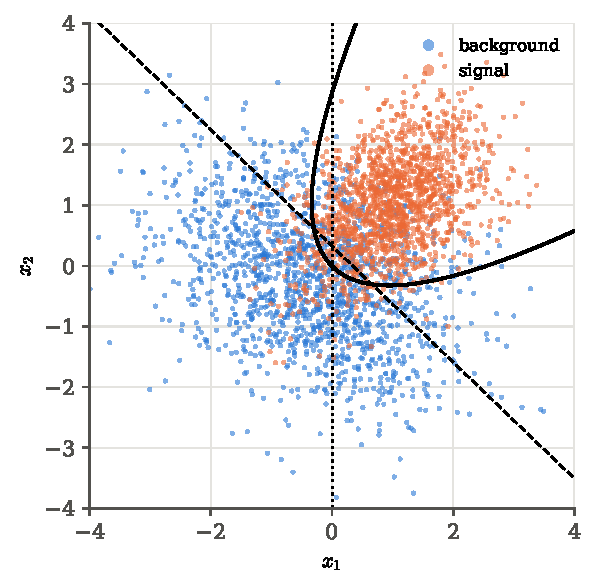
\includegraphics[width=0.6\linewidth]{figures/ch04/np_scatter.pdf}
\caption{Signal (orange) and background (blue) events in two measured
variables, with three boundaries that each keep $90\%$ of the signal: a cut on
$x_1$ alone (dotted), Fisher's straight line (dashed), and the curved contour
of constant likelihood ratio (solid). The curved boundary follows the shape of
the two clouds, which have different orientations, and so admits the least
background.}
\label{4a:fig:np-scatter}
\end{figure}

The lemma claims that no selection does better than the likelihood ratio. To
check this, the script also draws
$300$ random quadratic selections $g(\bm x)=\bm x\T\bm A\bm x+\bm v\T\bm x>c$,
each tuned to keep $90\%$ of the signal. The best of them keeps a background
fraction $\FourANPbkgRandom$, above the likelihood ratio's $\FourANPbkgLR$.
(Because the true ratio here is itself quadratic, a random quadratic can come
close, but it cannot win.) \Cref{4a:fig:np-roc} shows the whole trade-off as
a \newterm{ROC curve} \unpack{background efficiency against signal efficiency,
as the cut is varied}. The likelihood-ratio curve lies below the others at every
signal efficiency.

\begin{figure}[htbp]
\centering
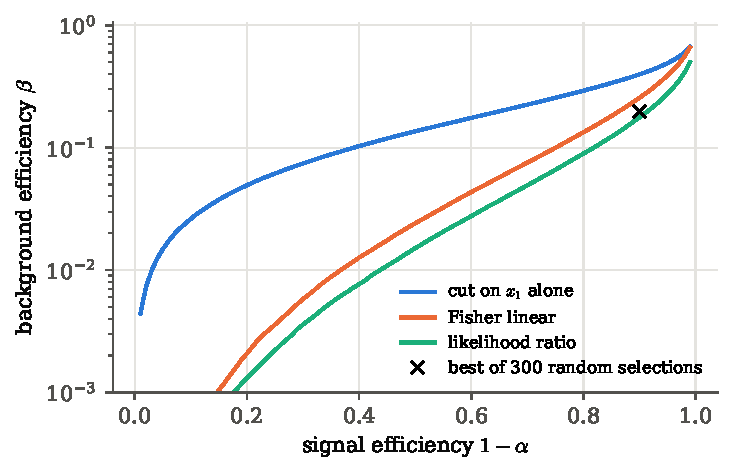
\includegraphics[width=0.8\linewidth]{figures/ch04/np_roc.pdf}
\caption{Background kept versus signal kept, as the threshold of each selection
is varied. Lower is better. The likelihood ratio (green) is lowest everywhere,
Fisher's linear discriminant (orange) is next, a cut on one variable (blue) is
worst, and the cross marks the best of $300$ random quadratic selections at
$90\%$ signal efficiency, which still lies above the green curve.}
\label{4a:fig:np-roc}
\end{figure}

\pyfile[firstline=32,lastline=50]{code/ch04/06_neyman_pearson.py}{Three selections compared at equal signal efficiency}

The function \pyname{lnr} is the log likelihood ratio, evaluated with the
exact densities because we generated the data; in a real analysis they would
come from simulation or be learned. Fisher's coefficients come from one line of
linear algebra, \pyname{np.linalg.solve(Wsum, tr_s.mean(0) - tr_b.mean(0))}, which is
\eqref{4a:eq:fisher-disc} without forming an inverse. For each statistic the
threshold for a given signal efficiency is a quantile of its signal
distribution (\pyname{np.quantile}), and the background efficiency is the
fraction of background above it, found by sorting.

\begin{pitfall}[Most powerful for one alternative only]
The Neyman--Pearson lemma is about \emph{two} completely specified
hypotheses. Real alternatives have free parameters: an unknown mass, an
unknown coupling. A test tuned to one mass hypothesis can be poor for another,
and a uniformly most powerful test rarely exists. The generalisation that
handles free parameters, by fitting them, is the likelihood-ratio test of the
next section; it is not guaranteed optimal, but it inherits the lemma's logic
and is the standard tool.
\end{pitfall}
\section{Likelihood-ratio tests and Wilks' theorem}
\label{4a:sec:wilks}

The Neyman--Pearson lemma needs two completely specified hypotheses. A real
search never has them. In the diphoton bump the background normalisation is
known only roughly, the signal strength is unknown, and even the null ``no
signal'' leaves the background level free. Such unknown parameters, which we
must allow for but do not want to report, are \newterm{nuisance parameters}
\unpack{parameters of the model that are not the question, like a background
level or a calibration constant}. We need a test that works with composite
hypotheses, and a way to get its null distribution without simulating every
possible value of the nuisance parameters.

The recipe is the natural generalisation of the lemma: in the ratio of
likelihoods, give each hypothesis its best shot by maximising over its free
parameters. The surprise, due to Wilks \cite{Wilks1938}, is that the resulting
statistic has, for large samples, a null distribution that does not depend on
the model at all.

\paragraph{The question in words.}
\begin{enumerate}[label=\arabic*.]
  \item How much better does the data fit if we free the parameters that the
        null fixes?
  \item How large must that improvement be before it is surprising, if the
        null is true?
  \item When does the universal answer fail, and what do we do then?
\end{enumerate}

\subsection{The likelihood-ratio statistic}
\label{4a:sec:lrt}

Let $\Like(\params)$ be the likelihood of the data as a function of all
parameters $\params\in\Theta$ (\cref{ch:03}), and let the null restrict them to
$\Theta_0\subset\Theta$. The \newterm{likelihood ratio} is
\begin{equation}
  \lambda(\bm x)=\frac{\sup_{\params\in\Theta_0}\Like(\params)}{\sup_{\params\in\Theta}\Like(\params)}
  =\frac{\Like(\hat{\params}_0)}{\Like(\hat{\params})},
  \qquad
  -2\ln\lambda=2\bigl[\ln\Like(\hat{\params})-\ln\Like(\hat{\params}_0)\bigr],
  \label{4a:eq:lrt}
\end{equation}
where $\hat{\params}$ is the maximum-likelihood estimate over all of $\Theta$
and $\hat{\params}_0$ the one restricted to $\Theta_0$. Because $\Theta_0$ is
part of $\Theta$, the restricted maximum can never be higher, so
$0<\lambda\le1$ and $-2\ln\lambda\ge0$. It is zero when the null fits as well
as anything, and grows as the unrestricted fit pulls away. We reject for large
$-2\ln\lambda$.

Two conventions need a word. First, \mainref{Def.~10.21} calls the quantity
$2\ln[\Like(\hat\params)/\Like(\hat\params_0)]$ itself ``$\lambda$'', so
Wasserman's $\lambda$ is our $-2\ln\lambda$. Second, the denominator maximises
over all of $\Theta$ rather than over the alternative alone,
$\Theta\setminus\Theta_0$. This changes the statistic very little and makes
its theory much simpler \mainref{p.~164}.

\begin{keyidea}[Wilks' theorem]
Let $\params$ have $r$ free parameters and the null fix $r-q$ of them, leaving
$q$ free. If the null is true, the model is regular and the true value lies in
the interior of $\Theta_0$, then for large samples
\[
  -2\ln\lambda\;\sim\;\chi^2_{r-q}
\]
\unpack{the degrees of freedom are the number of parameters the null fixes},
whatever the model \mainref{Thm~10.22}, \srcref{CasellaBerger}{Thm~10.3.3}.
The p-value is $\Prob(\chi^2_{r-q}>-2\ln\lambda_{\rm obs})$.
\end{keyidea}

For example, with five parameters and the null $\theta_4=\theta_5=0$, the
statistic is asymptotically $\chi^2_{5-3}=\chi^2_2$ \mainref{p.~164}. The
nuisance parameters, the ones left free under both hypotheses, cost nothing
in degrees of freedom: they are refitted in numerator and denominator.

\subsection{Why the answer is $\chi^2$}
\label{4a:sec:wilks-why}

Take one parameter, $\theta$, and a simple null $\theta=\theta_0$, so
$r-q=1$. Write $\ell(\theta)=\ln\Like(\theta)$ and expand it around its
maximum $\hat\theta$ \srcref{CasellaBerger}{p.~395}:
\begin{align}
  -2\ln\lambda
  &\eqby{1} 2\bigl[\ell(\hat\theta)-\ell(\theta_0)\bigr] \notag\\
  &\eqby{2} 2\Bigl[\ell(\hat\theta)-\Bigl(\ell(\hat\theta)+\ell'(\hat\theta)(\theta_0-\hat\theta)
            +\tfrac12\ell''(\hat\theta)(\theta_0-\hat\theta)^2+\dots\Bigr)\Bigr] \notag\\
  &\eqby{3} -\ell''(\hat\theta)\,(\hat\theta-\theta_0)^2+\dots \notag\\
  &\eqby{4} \Bigl(\frac{\hat\theta-\theta_0}{\widehat{\rm se}}\Bigr)^2+\dots .
  \label{4a:eq:wilks-taylor}
\end{align}
\begin{explain}
  \item Definition \eqref{4a:eq:lrt} with $\hat\theta_0=\theta_0$.
  \item Taylor expansion of $\ell(\theta_0)$ about $\hat\theta$.
  \item $\ell'(\hat\theta)=0$ at the maximum, and the $\ell(\hat\theta)$ terms
        cancel.
  \item The curvature of the log likelihood at its peak is the observed
        information, and its inverse is the variance of the estimate:
        $-\ell''(\hat\theta)=1/\widehat{\rm se}^{\,2}$ (\cref{ch:03}).
\end{explain}
For a large sample, $\hat\theta$ is approximately normal about the true value
with standard deviation se. Under the null the true value is $\theta_0$, so the
bracket in the last line is approximately a standard normal $Z$, and
$-2\ln\lambda\approx Z^2\sim\chi^2_1$. The dropped terms are of higher order in
$\hat\theta-\theta_0$, which shrinks as $1/\sqrt n$. In words: near its peak,
every smooth log likelihood is a parabola, the likelihood-ratio statistic is
the drop of that parabola between $\hat\theta$ and $\theta_0$, and the drop is
the square of the Wald statistic of \cref{4a:sec:wald}. With $k$ fixed
parameters the same expansion gives a quadratic form in a $k$-dimensional
normal vector weighted by its inverse covariance, which is a sum of $k$ squared
independent standard normals: $\chi^2_k$.

\paragraph{The linear-Gaussian case, where Wilks is exact.}
If the data are $y_i=\mu_i(\params)+\epsilon_i$ with known Gaussian errors
$\sigma_i$, then $-2\ln\Like(\params)=\chi^2(\params)+\text{const}$ with
$\chi^2(\params)=\sum_i(y_i-\mu_i(\params))^2/\sigma_i^2$ (\cref{ch:03}), and
\begin{equation}
  -2\ln\lambda
  \eqby{1} -2\ln\Like(\hat\params_0)+2\ln\Like(\hat\params)
  \eqby{2} \chi^2_{\min}(\Hnull)-\chi^2_{\min}(\Halt)
  \equiv\Delta\chi^2 .
  \label{4a:eq:delta-chi2}
\end{equation}
\begin{explain}
  \item Definition \eqref{4a:eq:lrt}.
  \item Maximising the likelihood is minimising $\chi^2$, and the constants
        cancel in the difference.
\end{explain}
When the model is linear in the parameters, $\Delta\chi^2$ is exactly
$\chi^2_{r-q}$ for any sample size. Here is the geometric reason. Divide each
residual by its $\sigma_i$; the noise vector $\bm\epsilon/\bm\sigma$ is then an
isotropic Gaussian in $N$ dimensions. A least-squares fit with $r$ linear
parameters is the orthogonal projection of the data onto an $r$-dimensional
subspace; the null's fit projects onto a $q$-dimensional subspace inside it.
Under the null, the difference of the two squared residual lengths is the
squared length of the noise projected onto the $(r-q)$-dimensional part of the
big subspace orthogonal to the small one. An isotropic Gaussian projected onto
any $k$-dimensional subspace is an isotropic Gaussian in $k$ dimensions, and its
squared length is $\chi^2_k$.

\paragraph{Example: the Poisson rate.}
With $X_1,\dots,X_n\iid\mathrm{Pois}(\lambda)$ and $\Hnull:\lambda=\lambda_0$
\srcref{CasellaBerger}{Ex.~10.3.2}, the log likelihood is
$\ell(\lambda)=-n\lambda+S\ln\lambda+\text{const}$ with $S=\sum_iX_i$, and its
maximum is at $\hat\lambda=S/n$. Then
\begin{align}
  -2\ln\lambda
  &\eqby{1} 2\bigl[\ell(\hat\lambda)-\ell(\lambda_0)\bigr]
   \eqby{2} 2\bigl[-n\hat\lambda+S\ln\hat\lambda+n\lambda_0-S\ln\lambda_0\bigr] \notag\\
  &\eqby{3} 2n\Bigl[(\lambda_0-\hat\lambda)-\hat\lambda\ln\frac{\lambda_0}{\hat\lambda}\Bigr] .
  \label{4a:eq:poisson-lrt}
\end{align}
\begin{explain}
  \item Definition, with a simple null.
  \item Insert $\ell$; the $\ln X_i!$ terms in the constant cancel.
  \item Use $S=n\hat\lambda$ and $\ln\hat\lambda-\ln\lambda_0=-\ln(\lambda_0/\hat\lambda)$.
\end{explain}
Casella and Berger simulate it for $\lambda_0=5$ and $n=25$. Our
$100\,000$ simulated experiments give the percentiles below; they sit close to
those of $\chi^2_1$ already at this modest sample size (their own table has
$1.630$, $2.726$, $3.744$ and $6.304$ from $10\,000$ experiments).
\begin{center}
\begin{tabular}{lcccc}
\toprule
percentile & $0.80$ & $0.90$ & $0.95$ & $0.99$ \\
\midrule
simulated $-2\ln\lambda$ & $\FourAWkSimEighty$ & $\FourAWkSimNinety$ & $\FourAWkSimNinetyfive$ & $\FourAWkSimNinetynine$ \\
$\chi^2_1$ & $\FourAWkChiEighty$ & $\FourAWkChiNinety$ & $\FourAWkChiNinetyfive$ & $\FourAWkChiNinetynine$ \\
\bottomrule
\end{tabular}
\end{center}

\paragraph{Example: is there a quadratic term?}
Twenty points $y_i$ at $x_i\in[-1,1]$ carry Gaussian noise of known
$\sigma=0.5$, and the truth is a constant. We fit a constant, a straight line
and a parabola $a+bx+cx^2$, and form $\Delta\chi^2$ for two nulls: $c=0$ (one
constraint) and $b=c=0$ (two constraints). Over $100\,000$ simulated data
sets the first has mean $\FourAWkMeanOne$ and variance $\FourAWkVarOne$, the
second mean $\FourAWkMeanTwo$ and variance $\FourAWkVarTwo$, matching
$\chi^2_1$ (mean $1$, variance $2$) and $\chi^2_2$ (mean $2$, variance $4$).
\Cref{4a:fig:wilks-checks} shows both examples.

\begin{figure}[htbp]
\centering
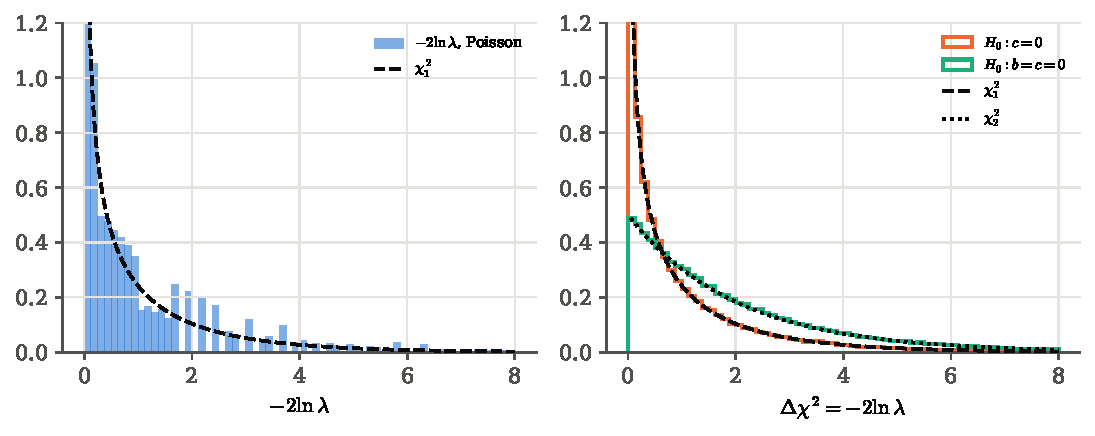
\includegraphics[width=\linewidth]{figures/ch04/wilks_checks.pdf}
\caption{Wilks' theorem checked twice. Left: the likelihood-ratio statistic for
a Poisson rate ($25$ counts, $\lambda_0=5$) follows the $\chi^2_1$ density
(dashed) closely. Right: $\Delta\chi^2$ between nested polynomial fits with
Gaussian noise follows $\chi^2_1$ when one coefficient is tested (orange) and
$\chi^2_2$ when two are (green, with the dotted density). For linear models the
agreement is exact, not only asymptotic.}
\label{4a:fig:wilks-checks}
\end{figure}

\paragraph{Example: Mendel's peas by likelihood ratio.}
Mendel counted $X=(315,101,108,32)$ peas in four classes, $n=556$, where his
theory predicts probabilities $p_0=(\frac9{16},\frac3{16},\frac3{16},\frac1{16})$
\mainref{Ex.~10.18}. The multinomial likelihood is $\prod_jp_j^{X_j}$, maximised
at $\hat p_j=X_j/n$, so
\begin{align*}
  -2\ln\lambda&=2\sum_{j=1}^4X_j\ln\frac{X_j/n}{p_{0j}}\\
  &=2\Bigl[315\ln\frac{315/556}{9/16}+101\ln\frac{101/556}{3/16}
   +108\ln\frac{108/556}{3/16}+32\ln\frac{32/556}{1/16}\Bigr]=0.48
\end{align*}
\mainref{Ex.~10.23}. The unrestricted model has three free probabilities (four
that sum to one), the null none, so the reference is $\chi^2_3$ and the p-value
is about $0.92$. The Pearson statistic of \cref{4a:sec:gof} gives $0.47$ on the
same data: for large counts the two statistics agree to second order.

\subsection{When the null sits on a boundary: $Z=\sqrt{q_0}$}
\label{4a:sec:boundary}

When the null value sits on the edge of the allowed region, Wilks' theorem
needs a correction, and the corrected answer is very simple. The case that
matters is the counting experiment of \cref{4a:sec:power-counting}: a count
$N\sim\mathrm{Pois}(s+b)$, with known expected background $b$, unknown
expected signal $s$, and the physical constraint $s\ge0$. The null $s=0$ sits
on the \emph{edge} of the allowed region, which breaks the interior condition
of Wilks' theorem.

\emph{The fit.} The log likelihood is
$\ell(s)=N\ln(s+b)-(s+b)+\text{const}$. Its maximum is at $s=N-b$ if that is
allowed, and at the boundary $s=0$ otherwise, so $\hat s=\max(N-b,0)$.

\emph{The statistic.} The discovery statistic is the likelihood-ratio
statistic \eqref{4a:eq:lrt} for the null $s=0$:
\begin{align}
  q_0=-2\ln\frac{\Like(0)}{\Like(\hat s)}
  &\eqby{1} 2\bigl[N\ln(\hat s+b)-(\hat s+b)-N\ln b+b\bigr] \notag\\
  &\eqby{2} \begin{cases}
              2\bigl[N\ln(N/b)-(N-b)\bigr], & N>b,\\
              0, & N\le b .
            \end{cases}
  \label{4a:eq:q0}
\end{align}
\begin{explain}
  \item Insert $\ell$ at $\hat s$ and at $0$.
  \item For $N>b$, $\hat s+b=N$. For $N\le b$ the best allowed fit is $\hat s=0$,
        the same as the null, and the ratio is one. A deficit is never evidence
        for a signal.
\end{explain}
\emph{Its null distribution.} For a large background, $N$ is nearly Gaussian
about $b$ and falls below it half of the time; then $q_0=0$. In the other
half, the unconstrained Wilks argument applies and $q_0$ is $\chi^2_1$. So the
null distribution is the
mixture $\frac12\delta(q_0)+\frac12\chi^2_1$, a result that goes back to
Chernoff. Its tail is
\begin{equation}
  \Prob(q_0\ge Z^2\given\Hnull)
  \eqby{1} \tfrac12\Prob\bigl(\chi^2_1\ge Z^2\bigr)
  \eqby{2} \tfrac12\Prob\bigl(\abs{Z'}\ge Z\bigr)
  \eqby{3} \Phi(-Z),
  \qquad Z'\sim\Normal(0,1),
  \label{4a:eq:half-chi2}
\end{equation}
\begin{explain}
  \item For $Z>0$ only the $\chi^2_1$ half contributes, with weight $\frac12$.
  \item A $\chi^2_1$ variable is the square of a standard normal.
  \item The two tails of $Z'$ are equal, $\Prob(\abs{Z'}\ge Z)=2\Phi(-Z)$.
\end{explain}
so the significance of an observation is simply $Z=\sqrt{q_0}$ standard
deviations \cite{Cowan2011}. The same half-$\chi^2$, and $Z=\sqrt{q_0}$, survive when the
background and calibrations are nuisance parameters profiled in $q_0$, as the second
part of the chapter shows in its section on discovery and exclusion with nuisance
parameters. \Cref{4a:fig:wilks-boundary} tests this with two
million background-only toys at $b=3.2$ and at $b=100$. The fraction with
$q_0=0$ is $\FourAWkZeroSmall$ and $\FourAWkZeroBig$, above one half because
the Poisson puts extra probability at and just below its mean. The fraction with
$q_0\ge9$, that is $Z\ge3$, is $\FourAWkThreeSmall$ and $\FourAWkThreeBig$,
against the asymptotic $\FourAWkThreeTh$: the formula is good to about $7\%$
at $b=100$ and to about $30\%$ at $b=3.2$. For Cowan's peak, $11$ events on
$3.2$, $Z=\sqrt{q_0}=\FourAWkZwilks$, while the exact Poisson tail corresponds
to $\FourAWkZexact$.

\begin{figure}[htbp]
\centering
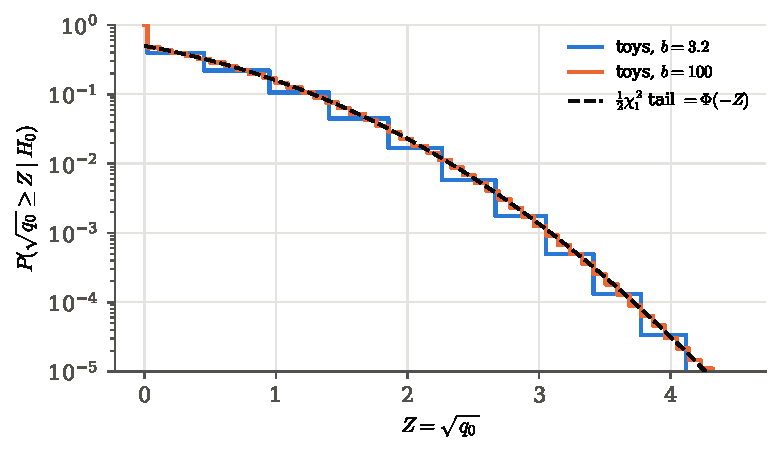
\includegraphics[width=0.8\linewidth]{figures/ch04/wilks_boundary.pdf}
\caption{The probability that background alone reaches a significance
$Z=\sqrt{q_0}$ or more, from toys with $b=3.2$ (blue) and $b=100$ (orange),
compared with the asymptotic half-$\chi^2_1$ prediction $\Phi(-Z)$ (dashed). The
large-background staircase follows the prediction closely; the small-background
one jumps in coarse steps because only integer counts are possible, and
wanders above and below the line.}
\label{4a:fig:wilks-boundary}
\end{figure}

\pyfile[firstline=65,lastline=70]{code/ch04/07_wilks.py}{The discovery statistic for a counting experiment}

The function is \eqref{4a:eq:q0} verbatim: the \pyname{np.where} enforces
$\hat s\ge0$, and the \pyname{errstate} guard silences the harmless warnings
from $\ln0$ in the branch that is discarded.

\paragraph{Example: the expected significance, and when $s/\sqrt b$ is enough.}
Before an experiment we want its \emph{median} significance if a signal $s$ is
present. We can get it without simulation \cite{Cowan2011}: evaluate $q_0$ on
the ``Asimov'' data set, in which $N$ is replaced by its expectation $s+b$.
Then
\begin{align}
  Z_A^2=q_0\bigl(N=s+b\bigr)
  &\eqby{1} 2\Bigl[(s+b)\ln\frac{s+b}{b}-s\Bigr]
   \eqby{2} 2\Bigl[(s+b)\ln\Bigl(1+\frac sb\Bigr)-s\Bigr] \notag\\
  &\eqby{3} 2\Bigl[(s+b)\Bigl(\frac sb-\frac{s^2}{2b^2}+\frac{s^3}{3b^3}-\dots\Bigr)-s\Bigr] \notag\\
  &\eqby{4} \frac{s^2}{b}\Bigl[1-\frac{s}{3b}+\dots\Bigr] .
  \label{4a:eq:asimov}
\end{align}
\begin{explain}
  \item \eqref{4a:eq:q0} with $N=s+b>b$; $N-b=s$.
  \item $(s+b)/b=1+s/b$.
  \item $\ln(1+u)=u-u^2/2+u^3/3-\dots$ with $u=s/b$.
  \item Multiply out: $(s+b)(s/b)=s^2/b+s$, whose $s$ cancels the $-s$;
        $(s+b)(-s^2/2b^2)=-s^2/2b-s^3/2b^2$; $(s+b)(s^3/3b^3)=s^3/3b^2+\dots$.
        Collecting, $s^2/b-s^2/2b=s^2/2b$ and $-s^3/2b^2+s^3/3b^2=-s^3/6b^2$;
        the factor $2$ gives $s^2/b-s^3/3b^2$.
\end{explain}
So for $s\ll b$ the familiar $Z\approx s/\sqrt b$ is recovered, and the first
correction shows it \emph{overestimates} the significance. With $s=10$ on
$b=100$, $Z_A=\FourAWkZAbig$, $s/\sqrt b=\FourAWkZsbBig$, and the median of
toy significances is $\FourAWkZmedBig$. With $s=5$ on $b=3.2$ the shortcut
fails badly: $Z_A=\FourAWkZAsmall$ against $s/\sqrt b=\FourAWkZsbSmall$.

\begin{inpractice}[Profile likelihood ratios at the LHC]
The discovery of the Higgs boson and most searches since use exactly this
statistic, with many nuisance parameters for backgrounds, luminosity and
energy scales. Each is ``profiled'': maximised separately in numerator and
denominator of $\lambda$. The asymptotic formulae, $Z=\sqrt{q_0}$ and the Asimov
median, are derived for this general case in \cite{Cowan2011}. Our toys
\emph{verify} them against an analytic answer. In research the same toys are the
\emph{instrument}: where counts are small, parameters sit on boundaries or the
signal mass is scanned, the null distribution of $q_0$ is generated by
simulation, and the asymptotic formula serves only as a cross-check.
\end{inpractice}

\paragraph{Where Wilks does not apply.}
Three conditions carried the derivation, and each fails somewhere in physics.
The parameter must be in the interior (the boundary gives the half-$\chi^2$
above). The hypotheses must be nested, one a special case of the other. And
every parameter of the alternative must mean something under the null. The last
condition fails in a bump hunt: the signal mass is meaningless when the signal
strength is zero, and maximising over it inflates $q_0$ beyond any $\chi^2$.
That is the look-elsewhere effect in its likelihood form
\cite{GrossVitells2010}, and it leads to the trials factor treated in the second part of the chapter.
\section{Goodness of fit: Pearson's $\chi^2$ and Kolmogorov--Smirnov}
\label{4a:sec:gof}

So far the null has always been tested against a definite direction: a
signal in a window, a bias of a coin, a shift of a calibration. Often we want
something vaguer. Here is the background model for the whole mass spectrum,
thirty bins of it; does it describe the data \emph{at all}? No particular
alternative is in mind, just ``something else''. This is a
\newterm{goodness-of-fit} test \srcref{Cowan}{\S4.5}: the test statistic
itself measures the disagreement between data and model, and its large values
are the extreme direction.

\paragraph{The question in words.}
\begin{enumerate}[label=\arabic*.]
  \item How do we add up the disagreement of many bins into one number with a
        known null distribution?
  \item What changes when the total is fixed, when parameters were fitted to
        the same data, and when counts are small?
  \item Can we avoid binning altogether?
\end{enumerate}

\subsection{The $\chi^2$ distribution, recalled}
\label{4a:sec:chi2-dist}

If $Z_1,\dots,Z_k$ are independent standard normals, $V=\sum_{i=1}^kZ_i^2$ has
the $\chi^2$ distribution with $k$ degrees of freedom (\cref{ch:02}), with
density, mean and variance \mainref{p.~159}
\begin{equation}
  f(v)=\frac{v^{k/2-1}e^{-v/2}}{2^{k/2}\Gamma(k/2)}\quad(v>0),
  \qquad
  \E V=k,\qquad \Var V=2k .
  \label{4a:eq:chi2-density}
\end{equation}
The mean is immediate, $\E Z_i^2=1$ for each term, and the variance follows
from $\E Z^4=3$: $\Var Z_i^2=3-1=2$ per term. Its upper quantile
$\chi^2_{k,\alpha}$ is defined by $\Prob(\chi^2_k>\chi^2_{k,\alpha})=\alpha$, and
a p-value is the upper tail beyond the observed value. For large $k$ the
distribution is close to $\Normal(k,2k)$.

\subsection{Pearson's statistic}
\label{4a:sec:pearson}

A histogram has $N$ bins with observed counts $n_i$ and expected counts
$\nu_i$ under the model. If the counts are independent Poisson variables and
none of the $\nu_i$ is small, each $n_i$ is approximately Gaussian with mean
$\nu_i$ and variance $\nu_i$, so $(n_i-\nu_i)/\sqrt{\nu_i}$ is approximately a
standard normal. Adding the squares \srcref{Cowan}{(4.39)},
\begin{equation}
  \chi^2=\sum_{i=1}^N\frac{(n_i-\nu_i)^2}{\nu_i}\;\sim\;\chi^2_N
  \qquad\text{(approximately, for }\nu_i\gtrsim5\text{)} .
  \label{4a:eq:pearson-poisson}
\end{equation}
The approximation does not care what physical variable was histogrammed or
what shape the model has; the test is \newterm{distribution free}. Each term is
the squared deviation in units of its own standard deviation, so $\chi^2$ is
the total disagreement counted in ``sigmas squared''.

If instead the total $n=\sum_in_i$ is fixed, the counts are multinomial with
cell probabilities $p_{0i}$ and expected counts $E_i=np_{0i}$, and Pearson's
statistic is \mainref{Def.~10.16}, \srcref{Cowan}{(4.41)}
\begin{equation}
  T=\sum_{j=1}^k\frac{(X_j-E_j)^2}{E_j}\;\sim\;\chi^2_{k-1}
  \label{4a:eq:pearson-multinomial}
\end{equation}
under the null, asymptotically \mainref{Thm~10.17}. The one lost degree of
freedom is the constraint $\sum_j(X_j-E_j)=0$: the deviations are not
independent, because an excess in one cell must be paid for by deficits
elsewhere. The case $k=2$ shows the mechanism exactly. With cell
probabilities $p$ and $1-p$, $X_2-n(1-p)=-(X_1-np)$, so
\begin{align}
  T
  &\eqby{1} \frac{(X_1-np)^2}{np}+\frac{(X_1-np)^2}{n(1-p)} \notag\\
  &\eqby{2} (X_1-np)^2\,\frac{(1-p)+p}{np(1-p)}
   \eqby{3} \Bigl(\frac{X_1-np}{\sqrt{np(1-p)}}\Bigr)^2 .
  \label{4a:eq:pearson-two}
\end{align}
\begin{explain}
  \item The second deviation is minus the first, and its square is the same.
  \item Common denominator.
  \item $(1-p)+p=1$.
\end{explain}
The bracket is the binomial count standardised by its own mean $np$ and
standard deviation $\sqrt{np(1-p)}$, which by the de Moivre--Laplace theorem of
\cref{ch:02} is approximately standard normal. So $T\approx Z^2\sim\chi^2_1$:
two cells, one degree of freedom. For $k$ cells the same happens in $k-1$
dimensions: the constraint confines the standardised deviation vector to a
hyperplane, and its squared length is a sum of $k-1$ independent squared
normals.

\paragraph{Example: Mendel's peas.}
Mendel crossed peas and counted $X=(315,101,108,32)$ progeny of four types,
$n=556$; his theory predicts $p_0=(\frac9{16},\frac3{16},\frac3{16},\frac1{16})$
\mainref{Ex.~10.18}. The expected counts are $E=(312.75,104.25,104.25,34.75)$
and
\begin{align*}
  T&=\frac{(315-312.75)^2}{312.75}+\frac{(101-104.25)^2}{104.25}
     +\frac{(108-104.25)^2}{104.25}+\frac{(32-34.75)^2}{34.75}\\
   &=0.016+0.101+0.135+0.218=\FourAMendelChi .
\end{align*}
With $k-1=3$ degrees of freedom the $5\%$ critical value is $7.815$, far above,
and the p-value is $\Prob(\chi^2_3>\FourAMendelChi)=\FourAMendelP$. So the data
do not contradict Mendel's theory. They do not prove it either. A test like
this can show evidence to reject the null, but it cannot prove the null
\mainref{p.~161}, because a failure to reject may come from a true null or
from low power. (A footnote there recalls that Mendel's results have been
suspected of fitting \emph{too} well. A p-value very close to one is also
improbable under the null.)

\begin{pitfall}[$\chi^2/\nu$ near one is not enough]
It is common to quote $\chi^2$ divided by the number of degrees of freedom and
call anything near one a good fit. The ratio hides the scale: the spread of
$\chi^2_\nu/\nu$ is $\sqrt{2/\nu}$, which shrinks with $\nu$. For
$\chi^2=15$ on $10$ degrees of freedom the p-value is $0.13$, perfectly fine;
for $\chi^2=150$ on $100$, the same ratio, it is $9.0\times10^{-4}$
\srcref{Cowan}{p.~62}. Always quote $\chi^2$ and $\nu$ separately, or the
p-value.
\end{pitfall}

\subsection{Fitted parameters and small counts}
\label{4a:sec:gof-fitted}

Usually the model has parameters, such as a background slope, that are
estimated from the same histogram. The fit pulls the expectation towards the
data and makes $\chi^2$ smaller than it would be at the true parameters. If
$s$ parameters are estimated by maximising the multinomial likelihood of the
binned counts, $Q(\params)=\prod_jp_j(\params)^{N_j}$, then
\mainref{Thm~10.29}
\begin{equation}
  Q=\sum_{j=1}^k\frac{\bigl(N_j-np_j(\hat\params)\bigr)^2}{np_j(\hat\params)}
  \;\sim\;\chi^2_{k-1-s} :
  \label{4a:eq:pearson-fitted}
\end{equation}
each fitted parameter removes one degree of freedom, for the same geometric
reason as in Wilks' theorem (\cref{4a:sec:wilks-why}): the fit projects the
deviations onto a smaller subspace. This count holds only when the parameters
are fitted to the binned counts. If they are estimated instead from the
\emph{unbinned} data, which is often more natural, the distribution of $Q$ is
no longer $\chi^2_{k-1-s}$; a theorem of Chernoff and Lehmann puts it between
$\chi^2_{k-1-s}$ and $\chi^2_{k-1}$ \mainref{p.~169}. The reason is that the
unbinned estimate is not tuned to the bins, so it removes less of the
disagreement.

\paragraph{Example: fitting a decay length.}
The script \pyname{code/ch04/08_goodness_of_fit.py} draws $400$ decay times
with mean $\tau=2$, histograms them in $k=8$ bins, $[0,1),[1,2),\dots,[7,\infty)$,
and fits $\tau$ two ways: by maximising the binned multinomial likelihood, and
by the unbinned maximum-likelihood estimate $\hat\tau=\bar t$. Over $4000$
repetitions the mean of $Q$ is $\FourAGofMeanBinned$ with the binned fit, as
$\chi^2_{k-2}=\chi^2_6$ predicts, and $\FourAGofMeanRaw$ with the unbinned
one; each mean carries a random error of about $\FourAGofMeanErr$. Both fits see
the same histograms, so their difference is measured much better: the unbinned fit
leaves $Q$ larger by $\FourAGofMeanDiff\pm\FourAGofMeanDiffErr$ on average, which
puts it between $\chi^2_6$ and $\chi^2_7$, as Chernoff--Lehmann says
(\cref{4a:fig:gof-chi2}, right). Here the difference is small; it matters more
when the bins are few and the parameters many.

\paragraph{Example: when the bins are sparse.}
The $\chi^2_N$ approximation needs every $\nu_i$ to be reasonably large. With a
few counts per bin, $(n_i-\nu_i)^2/\nu_i$ is far from a squared Gaussian: a
Poisson with small mean is skewed, and a single count of $5$ where $1$ was
expected contributes $16$. \srcref{Cowan}{p.~63} finds $\chi^2=29.8$ for $20$
bins of his bump histogram, where most bins have fewer than five entries, and
shows that the $\chi^2_{20}$ tail ($0.073$) understates the true p-value
($0.11$, from Monte Carlo). Our version uses $20$ Poisson bins with expected
counts between about $1$ and $4$. Simulating $200\,000$ histograms under the
null, the $95\%$ point of Pearson's statistic is $\FourAGofQsmall$, against
$\FourAGofQth$ for $\chi^2_{20}$. For an observed value of $30$ the simulated
p-value is $\FourAGofPsmallMC$ and the $\chi^2$ formula would give
$\FourAGofPsmallChi$. With $25$ times more data in the same shape the
simulated $95\%$ point becomes $\FourAGofQlarge$, on the $\chi^2$ value
(\cref{4a:fig:gof-chi2}, left). The remedy is Cowan's: when counts are small,
simulate the null distribution of the statistic you computed.

\begin{figure}[htbp]
\centering
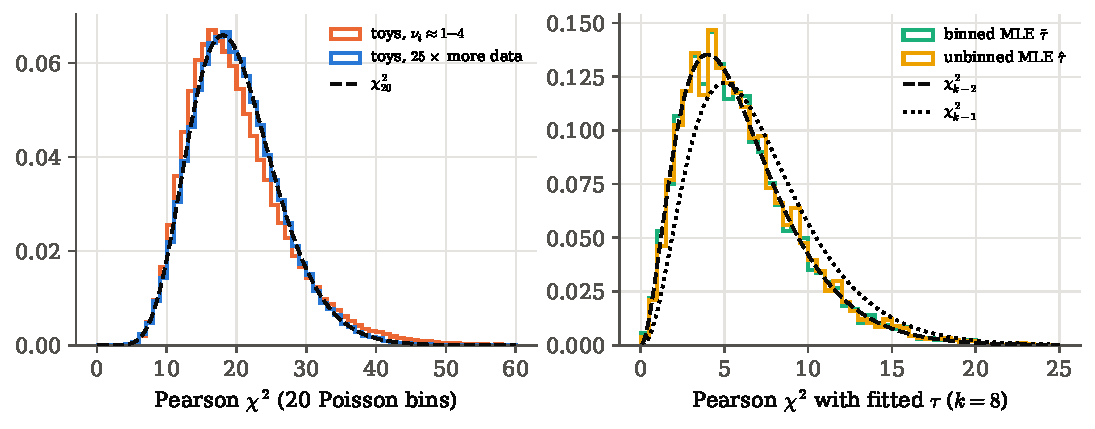
\includegraphics[width=\linewidth]{figures/ch04/gof_chi2.pdf}
\caption{Left: the null distribution of Pearson's $\chi^2$ for $20$ Poisson
bins. With one to four expected counts per bin (orange) it has a longer tail
than $\chi^2_{20}$ (dashed); with $25$ times more data (blue) it lies on the
curve. Right: after fitting a decay length, Pearson's statistic follows
$\chi^2_{k-2}$ when the fit uses the binned counts (green) and sits slightly
towards $\chi^2_{k-1}$ (dotted) when the fit uses the unbinned decay times
(yellow).}
\label{4a:fig:gof-chi2}
\end{figure}

Binning is a choice, and different choices give different p-values
\srcref{Cowan}{p.~63}. Bins must be wide enough for the approximation, yet wide
bins throw away where in the bin each event fell. Simulating the null
distribution relaxes the first constraint. Avoiding bins altogether removes
the choice.

\subsection{The Kolmogorov--Smirnov test}
\label{4a:sec:ks}

For $n$ individual measurements $x_1,\dots,x_n$ we can compare the data with a
hypothesised continuous CDF $F$ directly. The \newterm{empirical CDF}
\unpack{the fraction of the data at or below $x$}
\[
  F_n(x)=\frac1n\#\{i:\ x_i\le x\}
\]
is a staircase that climbs by $1/n$ at each data point. The
\newterm{Kolmogorov--Smirnov statistic} is its largest vertical distance from
the model,
\begin{equation}
  D_n=\sup_x\abs{F_n(x)-F(x)} .
  \label{4a:eq:ks}
\end{equation}
The supremum over all $x$ reduces to a check at the data points. Sort them,
$x_{(1)}\le\dots\le x_{(n)}$. Between two data points $F_n$ is flat and $F$
increases, so the gap $F_n-F$ is largest just after a jump and $F-F_n$ is
largest just before one. At $x_{(i)}$ the staircase jumps from $(i-1)/n$ to
$i/n$, hence
\begin{equation}
  D_n=\max\bigl(D_n^+,D_n^-\bigr),\qquad
  D_n^+=\max_i\Bigl(\frac in-F(x_{(i)})\Bigr),\qquad
  D_n^-=\max_i\Bigl(F(x_{(i)})-\frac{i-1}n\Bigr).
  \label{4a:eq:ks-compute}
\end{equation}

Why is the null distribution of $D_n$ the same for every continuous $F$? Set
$u_i=F(x_i)$. Under the null the $u_i$ are uniform on $(0,1)$ by the
probability integral transform of \cref{4a:sec:p-uniform}, and because $F$ is
increasing, ``$x_i\le x$'' is the same as ``$u_i\le F(x)$''. Writing $u=F(x)$,
\begin{equation}
  \abs{F_n(x)-F(x)}
  \eqby{1} \Bigl\lvert\frac1n\#\{i:u_i\le u\}-u\Bigr\rvert
  \eqby{2} \abs{G_n(u)-u},
  \label{4a:eq:ks-free}
\end{equation}
\begin{explain}
  \item Replace each event $x_i\le x$ by the equivalent $u_i\le u$.
  \item $G_n$ is the empirical CDF of the uniform sample $u_1,\dots,u_n$.
\end{explain}
so $D_n$ is the Kolmogorov--Smirnov distance of a uniform sample from the
uniform CDF, whatever $F$ was. Its distribution can be tabulated once; for
large $n$, Kolmogorov showed that $\sqrt nD_n$ converges to a limiting
distribution with tail $\Prob(K>x)=2\sum_{j\ge1}(-1)^{j-1}e^{-2j^2x^2}$.

\paragraph{Example: a decay length that is not what we thought.}
Fifty decay times are drawn with mean $1.3$, and we test the null that the
mean is $1$, $F(x)=1-e^{-x}$. \Cref{4a:fig:ks} (left) shows the empirical
staircase below the model curve over most of the range, since longer lifetimes
make small times rarer. Our own implementation of \eqref{4a:eq:ks-compute}
finds $D_{50}=\FourAKsD$, so $\sqrt nD_n=\FourAKsSqrtnD$. The exact p-value
from \pyname{scipy.stats.kstest} (which also returns $D=\FourAKsDscipy$) is
$\FourAKsPscipy$; the Kolmogorov limit gives $\FourAKsPkolm$; and $40\,000$
simulated null samples of size $50$ give $\FourAKsPmc$. With only fifty events,
a $30\%$ change of lifetime gives modest evidence against the null at best, and
another fifty decays could easily give a much larger p-value.

\begin{figure}[htbp]
\centering
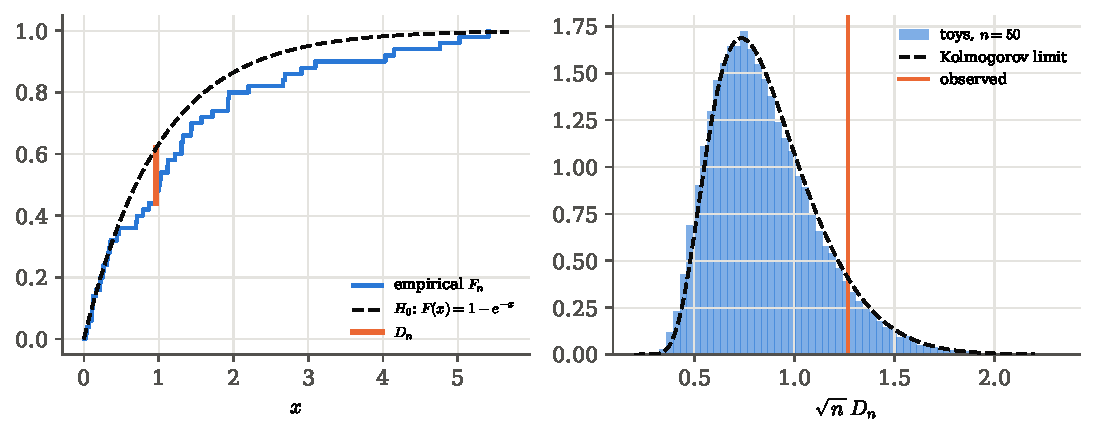
\includegraphics[width=\linewidth]{figures/ch04/ks_test.pdf}
\caption{Left: the empirical CDF of fifty decay times (blue staircase) and the
null model's CDF (dashed). The orange bar marks the largest vertical gap,
$D_n$. Right: the null distribution of $\sqrt n\,D_n$ for samples of fifty,
from simulation (histogram) and Kolmogorov's large-$n$ limit (dashed), with the
observed value marked.}
\label{4a:fig:ks}
\end{figure}

\pyfile[firstline=85,lastline=91]{code/ch04/08_goodness_of_fit.py}{The Kolmogorov--Smirnov statistic from scratch}

The function sorts the sample, evaluates the model CDF at each point, and
takes the two maxima of \eqref{4a:eq:ks-compute} with the vectors
\pyname{np.arange(1, n+1)/n} (the tops of the steps) and
\pyname{np.arange(0, n)/n} (the bottoms). It agrees with scipy to every digit
printed. The Monte Carlo p-value calls the same function on samples drawn from
the null.

Two cautions. The distribution-free property holds only when $F$ is fully
specified in advance. If its parameters are estimated from the same data, the
fitted CDF hugs the data and $D_n$ is typically smaller, so the tabulated
p-values are too large; the null distribution must then be simulated, fitting
the parameters afresh on each simulated sample. And like every goodness-of-fit
test, a large p-value does not certify the model: it may only mean the test has
little power against the departure that is actually present
\mainref{p.~169}. Relatives of KS that weight the whole curve rather than its
largest gap, such as the Cram\'er--von Mises statistic, are often more
powerful \srcref{Cowan}{p.~63}.
\section{From $p$ to $Z\sigma$, and why a discovery needs $5\sigma$}
\label{4a:sec:ztable}

Particle physicists rarely quote p-values. They say that an excess is ``a
$2.6\sigma$ fluctuation'', that $3\sigma$ counts as evidence, and that a
discovery needs $5\sigma$. The language comes from Gaussian error bars, but it
is used for every kind of test statistic, including Poisson counts and
likelihood ratios that are nothing like Gaussian. So ``$Z$ sigma'' must be a
relabelling of the p-value, and it is: a precise one-to-one translation. Once
we have it, we can ask why particle physics sets the bar so high, when other
fields are content with $p<0.05$.

\paragraph{The question in words.}
\begin{enumerate}[label=\arabic*.]
  \item What exactly does ``$Z$ sigma'' mean for a test statistic that is not
        Gaussian?
  \item How small is the p-value of a $5\sigma$ result, and how does it
        compare with $3\sigma$?
  \item What goes wrong with a lower threshold, given many searches, imperfect
        backgrounds and new physics that is rare?
\end{enumerate}

\subsection{The translation}
\label{4a:sec:p-to-z}

The \newterm{significance} $Z$ of a p-value is the number of standard
deviations above the mean at which a standard normal variable has the same
upper-tail probability \cite{Cowan2011}:
\begin{equation}
  p=\int_Z^\infty\frac{e^{-t^2/2}}{\sqrt{2\pi}}\,\dd t=1-\Phi(Z)=\Phi(-Z),
  \qquad
  Z=\Phi^{-1}(1-p) .
  \label{4a:eq:p-to-z}
\end{equation}
The definition says nothing about the distribution of the actual statistic. A
Poisson count, a $\chi^2$, a permutation statistic: whatever gave the p-value,
$Z$ is only a relabelling of it on a scale that physicists find intuitive. For
the bump of \cref{4a:sec:bump}, $p=\FourABumpP$ becomes $Z=\FourABumpZ$. Some
authors use the two-sided convention $p=2\Phi(-Z)$, which corresponds to
$\abs{\text{Gaussian}}\ge Z$; discovery claims use the one-sided version,
because only an excess counts. The table from
\pyname{code/ch04/09_p_to_z.py}:
\begin{center}
\begin{tabular}{ccc}
\toprule
$Z$ & one-sided $\Phi(-Z)$ & two-sided $2\Phi(-Z)$ \\
\midrule
$1$ & $\FourAPzOneOne$ & $\FourAPzOneTwo$ \\
$2$ & $\FourAPzTwoOne$ & $\FourAPzTwoTwo$ \\
$3$ & $\FourAPzThreeOne$ & $\FourAPzThreeTwo$ \\
$4$ & $\FourAPzFourOne$ & $\FourAPzFourTwo$ \\
$5$ & $\FourAPzFiveOne$ & $\FourAPzFiveTwo$ \\
$6$ & $\FourAPzSixOne$ & $\FourAPzSixTwo$ \\
\bottomrule
\end{tabular}
\end{center}
In the other direction, $p=0.05$ corresponds to $Z=\FourAPzZfivepct$
one-sided and $\FourAPzZfivepctTwo$ two-sided. The usual $5\%$ threshold of
the life sciences is a $1.6$ to $2\sigma$ effect, and a $5\sigma$ result has a
p-value about $170\,000$ times smaller.

\paragraph{Example: reading the scale in both directions.}
A search reports a one-sided p-value of $2.5\times10^{-4}$. Then
$Z=\Phi^{-1}(1-2.5\times10^{-4})=3.48$, a little above the $3\sigma$ line of
``evidence'' and well short of $5\sigma$. Had the same number been a
two-sided p-value, the one-sided tail would be half of it, $1.25\times10^{-4}$,
and $Z=3.66$; quoting $Z$ without saying which convention is in use can move
the claim by a fifth of a sigma. In the other direction, an analysis planned
to reach $Z=4.2$ must see a background-only tail no bigger than
$\Phi(-4.2)=1.3\times10^{-5}$, about one chance in $75\,000$.

\paragraph{How fast the tail falls.}
For large $Z$ there is a simple estimate of the tail, useful for checking
orders of magnitude without a table. Write $\varphi(t)=e^{-t^2/2}/\sqrt{2\pi}$
and note that $\varphi'(t)=-t\varphi(t)$. Integrating by parts,
\begin{align}
  \Phi(-Z)=\int_Z^\infty\varphi(t)\,\dd t
  &\eqby{1} \int_Z^\infty\frac1t\,\bigl(t\varphi(t)\bigr)\dd t
   \eqby{2} \Bigl[-\frac{\varphi(t)}{t}\Bigr]_Z^\infty-\int_Z^\infty\frac{\varphi(t)}{t^2}\,\dd t \notag\\
  &\eqby{3} \frac{\varphi(Z)}{Z}-\int_Z^\infty\frac{\varphi(t)}{t^2}\,\dd t
   \relby{4}{\approx} \frac{\varphi(Z)}{Z}\Bigl(1-\frac1{Z^2}\Bigr) .
  \label{4a:eq:mills}
\end{align}
\begin{explain}
  \item Multiply and divide by $t$.
  \item Parts, with $u=1/t$ and $\dd v=t\varphi(t)\,\dd t$, so $v=-\varphi(t)$
        and $\dd u=-\dd t/t^2$.
  \item The boundary term vanishes at infinity.
  \item The remaining integral is smaller by a factor of about $1/Z^2$; the
        same trick applied to it gives the correction shown.
\end{explain}
At $Z=5$, $\varphi(5)=e^{-12.5}/\sqrt{2\pi}=1.49\times10^{-6}$, so the
estimate is $1.49\times10^{-6}\times0.96/5=2.85\times10^{-7}$, against the
exact $\FourAPzFiveOne$. The factor $e^{-Z^2/2}$ dominates: each extra sigma near
$Z=5$ costs a factor of $e^{-(Z+1)^2/2+Z^2/2}=e^{-Z-1/2}\approx250$ in
probability.

\begin{figure}[htbp]
\centering
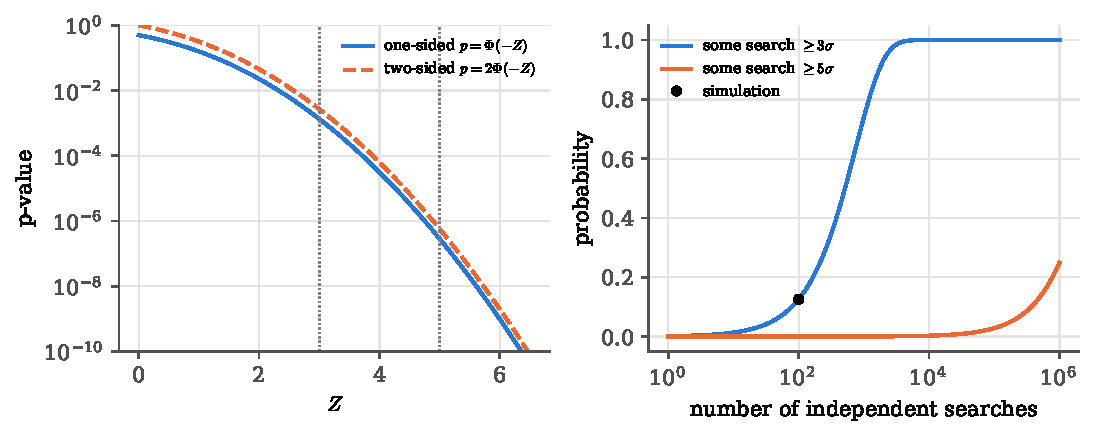
\includegraphics[width=\linewidth]{figures/ch04/p_to_z.pdf}
\caption{Left: the p-value that corresponds to a significance $Z$, one-sided
(solid) and two-sided (dashed), on a log scale; the dotted lines mark $3\sigma$
and $5\sigma$. Right: the probability that at least one of many independent
background-only searches reaches $3\sigma$ (blue) or $5\sigma$ (orange). With a
hundred searches the chance of a $3\sigma$ fluctuation somewhere is already
about one in eight; the black dot is a direct simulation.}
\label{4a:fig:p-to-z}
\end{figure}

\subsection{Why five}
\label{4a:sec:why-five}

Three separate arguments each call for a threshold far stricter than
$p<0.05$: there are many searches, the backgrounds are imperfect, and new
physics is rare. We take them one at a time.

\paragraph{Many searches.}
A laboratory does not run one test. It scans masses, channels, final states,
and every analysis group does the same. If $N$ independent searches each have
probability $p_1$ of a false alarm, the probability that at least one of them
fires is
\begin{equation}
  \Prob(\text{at least one})
  \eqby{1} 1-\Prob(\text{none})
  \eqby{2} 1-(1-p_1)^N
  \relby{3}{\approx} Np_1\quad(Np_1\ll1).
  \label{4a:eq:any-search}
\end{equation}
\begin{explain}
  \item Complement.
  \item Independence: the probability that all $N$ stay quiet is the product.
  \item $(1-p_1)^N\approx1-Np_1$ to first order.
\end{explain}
With $N=100$ and a $3\sigma$ threshold, $p_1=\FourAPzThreeOne$ gives
$\FourAPzAnyThree$, and a simulation of the maximum of $100$ standard normals
over $200\,000$ trials gives $\FourAPzAnyThreeMC$. One lab in eight would see a
$3\sigma$ effect from nothing. At $5\sigma$ the same number is
$\FourAPzAnyFive$. This is Kruschke's two coins of \cref{4a:sec:stopping}
on a larger scale, and it is the look-elsewhere effect that the second part of
the chapter quantifies properly for scans over a mass.

\paragraph{Imperfect backgrounds.}
The p-value is computed from the null model alone, so an error in the null
model goes straight into it. In \cref{4a:sec:poisson-p} moving the background
from $0.5$ to $0.8$ events changed the p-value of five events by a factor of
about eight. Real detectors also have tails in their resolution functions that
no Gaussian captures. A $5\sigma$ threshold leaves a margin: an effect that
survives it is unlikely to be an artefact of a background that is off by a
modest amount. A $3\sigma$ effect is not so robust.

\paragraph{New physics is rare.}
The third argument is the population argument of \cref{4a:sec:not-posterior},
and it needs Bayes' theorem. \emph{The event} is ``the search crossed the
threshold''. \emph{The question} is what produced it: a real effect, or a false
alarm on a null. Suppose that of all the hypotheses that searches test, only a
fraction $\pi_1=10^{-3}$ are real. \emph{Each route in turn:} when an effect
is real, the search reaches the threshold half the time, so the power is
$0.5$; when the null is true, it reaches it with the false-alarm probability
$p_{\rm thr}$ of the threshold. \Cref{4a:fig:tree} draws the probability tree.
\emph{Only then the numbers.} The fraction of threshold crossings that are
real, the \emph{purity} of the discoveries, is
\begin{equation}
  \Prob(\text{real}\given\text{crossed})
  \eqby{1} \frac{\pi_1\times0.5}{\pi_1\times0.5+(1-\pi_1)\,p_{\rm thr}} ,
  \label{4a:eq:purity-z}
\end{equation}
\begin{explain}
  \item Bayes' theorem on the tree: the two branches that end in ``crossed''
        are ``real, then detected'' and ``null, then false alarm''.
\end{explain}
exactly the purity formula \eqref{4a:eq:purity} of event selection, with
hypotheses in place of particles. With $p_{\rm thr}=\FourAPzThreeOne$ ($3\sigma$)
the purity is $\FourAPzPurThree$: nearly three quarters of the ``discoveries''
would be false. With $p_{\rm thr}=\FourAPzFiveOne$ ($5\sigma$) it is
$\FourAPzPurFive$. The numbers $\pi_1$ and the power are illustrative, and a
frequentist cannot even write $\pi_1$ into the p-value. But the lesson is
robust: when true effects are rare, the threshold must be far smaller than
$\pi_1$ for a crossing to mean what we want it to mean. Extraordinary claims
need extraordinary evidence, and $5\sigma$ is how particle physics encodes that
without writing down a prior. \Cref{ch:05} writes it down.

\begin{figure}[htbp]
\centering
\begin{tikzpicture}[
  grow=right, level distance=33mm,
  level 1/.style={sibling distance=22mm},
  level 2/.style={sibling distance=11mm},
  every node/.style={font=\small},
  edge from parent/.style={draw, thick, black!60}]
  \node[draw, rounded corners=2pt, fill=ideabg] {searched hypothesis}
    child {node[draw, rounded corners=2pt, fill=ideabg] (null) {null ($1-\pi_1$)}
      child {node (nq) {not crossed}}
      child {node[text=bdryred] (nc) {crossed: false alarm}}
    }
    child {node[draw, rounded corners=2pt, fill=ideabg] (real) {real ($\pi_1$)}
      child {node (rq) {not crossed}}
      child {node[text=tangentgreen!70!black] (rc) {crossed: discovery}}
    };
  \node[anchor=west, font=\footnotesize, text=black!70] at ($(nc.east)+(1mm,0)$) {prob.\ $p_{\rm thr}$};
  \node[anchor=west, font=\footnotesize, text=black!70] at ($(nq.east)+(1mm,0)$) {prob.\ $1-p_{\rm thr}$};
  \node[anchor=west, font=\footnotesize, text=black!70] at ($(rc.east)+(1mm,0)$) {prob.\ power};
  \node[anchor=west, font=\footnotesize, text=black!70] at ($(rq.east)+(1mm,0)$) {prob.\ $1-$power};
\end{tikzpicture}
\caption{The probability tree behind the $5\sigma$ convention. First nature
decides whether the hypothesis being searched for is real, with a small
probability $\pi_1$; then the experiment either crosses the threshold or not.
Among all crossings, the false alarms (red) come from the heavily populated
null branch, the discoveries (green) from the thin real branch. Only a tiny
false-alarm probability keeps the red leaf smaller than the green one.}
\label{4a:fig:tree}
\end{figure}

\paragraph{What $5\sigma$ does not say.}
A $5\sigma$ result has $p=\FourAPzFiveOne$. It does not follow that the
probability of the null is $\FourAPzFiveOne$, nor that the new particle exists
with probability $1-\FourAPzFiveOne$. As in \cref{4a:sec:not-posterior}, those
are inference-direction statements and need a prior. The convention in
particle physics is to call $3\sigma$ ``evidence'' and $5\sigma$ an
``observation'', to report the p-value (or $Z$) together with the expected
significance of the experiment, and to leave the probability of the hypothesis
to a Bayesian analysis.

\begin{recap}
\begin{itemize}
  \item The null hypothesis is the one whose sampling distribution we know:
        ``it happened by chance''. A test runs in the prediction direction,
        from $\Hnull$ to the outcomes it produces.
  \item The p-value is the probability, under $\Hnull$, of a test statistic at
        least as extreme as observed, in the direction the alternative
        predicts. The direction, and the experimental plan (stopping rule,
        number of places looked), are part of the question.
  \item A test has size $\alpha$ (false-alarm rate) and a power function
        $\beta(\theta)$ (rejection rate under the truth). Power grows with
        effect size and with $\sqrt n$; experiment planning is a power
        calculation.
  \item Under a continuous null the p-value is uniform, so ``reject if
        $p\le\alpha$'' has size $\alpha$. For discrete data it is valid:
        $\Prob(p\le\alpha)\le\alpha$.
  \item A p-value is not $\Prob(\Hnull\given\text{data})$: that needs the prior
        frequency of true nulls and the power (Bayes).
  \item Wald, t and permutation tests cover most everyday comparisons; the
        t-test is exact for small Gaussian samples, the permutation test for
        any distribution.
  \item Neyman--Pearson: for simple hypotheses the likelihood ratio is the most
        powerful statistic. With free parameters, $-2\ln\lambda$ is
        asymptotically $\chi^2$ with as many degrees of freedom as the null
        fixes (Wilks); on a boundary it is half $\chi^2_1$ and $Z=\sqrt{q_0}$.
  \item Pearson's $\chi^2$ and Kolmogorov--Smirnov test a whole model; fitted
        parameters, small counts and estimated CDFs change their null
        distributions, which can always be simulated.
  \item $Z=\Phi^{-1}(1-p)$. Discovery needs $5\sigma$ because of many searches,
        imperfect backgrounds and the rarity of real effects.
\end{itemize}
\end{recap}

\providecommand{\FourBKrN}{}\renewcommand{\FourBKrN}{24}
\providecommand{\FourBKrZ}{}\renewcommand{\FourBKrZ}{7}
\providecommand{\FourBKrThetaHat}{}\renewcommand{\FourBKrThetaHat}{0.292}
\providecommand{\FourBKrLo}{}\renewcommand{\FourBKrLo}{0.126}
\providecommand{\FourBKrHi}{}\renewcommand{\FourBKrHi}{0.511}
\providecommand{\FourBKrWaldLo}{}\renewcommand{\FourBKrWaldLo}{0.110}
\providecommand{\FourBKrWaldHi}{}\renewcommand{\FourBKrWaldHi}{0.474}
\providecommand{\FourBKrSe}{}\renewcommand{\FourBKrSe}{0.0928}
\providecommand{\FourBKrHoefEps}{}\renewcommand{\FourBKrHoefEps}{0.277}
\providecommand{\FourBKrHoefLo}{}\renewcommand{\FourBKrHoefLo}{0.014}
\providecommand{\FourBKrHoefHi}{}\renewcommand{\FourBKrHoefHi}{0.569}
\providecommand{\FourBKrPhalf}{}\renewcommand{\FourBKrPhalf}{0.064}
\providecommand{\FourBBWcovAll}{}\renewcommand{\FourBBWcovAll}{0.7498}
\providecommand{\FourBBWcovSame}{}\renewcommand{\FourBBWcovSame}{0.5005}
\providecommand{\FourBBWcovDiff}{}\renewcommand{\FourBBWcovDiff}{1.0000}
\providecommand{\FourBBWfracSame}{}\renewcommand{\FourBBWfracSame}{0.5009}
\providecommand{\FourBBeltCL}{}\renewcommand{\FourBBeltCL}{90}
\providecommand{\FourBBeltNobs}{}\renewcommand{\FourBBeltNobs}{6}
\providecommand{\FourBBeltLoSix}{}\renewcommand{\FourBBeltLoSix}{2.61}
\providecommand{\FourBBeltHiSix}{}\renewcommand{\FourBBeltHiSix}{11.84}
\providecommand{\FourBBeltMinAcc}{}\renewcommand{\FourBBeltMinAcc}{0.9002}
\providecommand{\FourBBeltMaxAcc}{}\renewcommand{\FourBBeltMaxAcc}{0.9995}
\providecommand{\FourBUpNinetyFiveZero}{}\renewcommand{\FourBUpNinetyFiveZero}{2.996}
\providecommand{\FourBUpNinetyZero}{}\renewcommand{\FourBUpNinetyZero}{2.303}
\providecommand{\FourBLoNinetyFiveThree}{}\renewcommand{\FourBLoNinetyFiveThree}{0.818}
\providecommand{\FourBUpNinetyFiveThree}{}\renewcommand{\FourBUpNinetyFiveThree}{7.75}
\providecommand{\FourBCBlo}{}\renewcommand{\FourBCBlo}{0.261}
\providecommand{\FourBCBhi}{}\renewcommand{\FourBCBhi}{1.184}
\providecommand{\FourBBeltLoZero}{}\renewcommand{\FourBBeltLoZero}{0.00}
\providecommand{\FourBBeltHiZero}{}\renewcommand{\FourBBeltHiZero}{3.00}
\providecommand{\FourBBeltLoOne}{}\renewcommand{\FourBBeltLoOne}{0.05}
\providecommand{\FourBBeltHiOne}{}\renewcommand{\FourBBeltHiOne}{4.74}
\providecommand{\FourBBeltLoTwo}{}\renewcommand{\FourBBeltLoTwo}{0.36}
\providecommand{\FourBBeltHiTwo}{}\renewcommand{\FourBBeltHiTwo}{6.30}
\providecommand{\FourBBeltLoThree}{}\renewcommand{\FourBBeltLoThree}{0.82}
\providecommand{\FourBBeltHiThree}{}\renewcommand{\FourBBeltHiThree}{7.75}
\providecommand{\FourBBeltLoFour}{}\renewcommand{\FourBBeltLoFour}{1.37}
\providecommand{\FourBBeltHiFour}{}\renewcommand{\FourBBeltHiFour}{9.15}
\providecommand{\FourBBeltLoFive}{}\renewcommand{\FourBBeltLoFive}{1.97}
\providecommand{\FourBBeltHiFive}{}\renewcommand{\FourBBeltHiFive}{10.51}
\providecommand{\FourBBeltLoSeven}{}\renewcommand{\FourBBeltLoSeven}{3.29}
\providecommand{\FourBBeltHiSeven}{}\renewcommand{\FourBBeltHiSeven}{13.15}
\providecommand{\FourBBeltLoEight}{}\renewcommand{\FourBBeltLoEight}{3.98}
\providecommand{\FourBBeltHiEight}{}\renewcommand{\FourBBeltHiEight}{14.43}
\providecommand{\FourBBeltLoNine}{}\renewcommand{\FourBBeltLoNine}{4.70}
\providecommand{\FourBBeltHiNine}{}\renewcommand{\FourBBeltHiNine}{15.71}
\providecommand{\FourBBeltLoTen}{}\renewcommand{\FourBBeltLoTen}{5.43}
\providecommand{\FourBBeltHiTen}{}\renewcommand{\FourBBeltHiTen}{16.96}
\providecommand{\FourBLadderMiss}{}\renewcommand{\FourBLadderMiss}{5}
\providecommand{\FourBLadderN}{}\renewcommand{\FourBLadderN}{10}
\providecommand{\FourBCovKnown}{}\renewcommand{\FourBCovKnown}{0.9498}
\providecommand{\FourBCovKnownErr}{}\renewcommand{\FourBCovKnownErr}{0.0005}
\providecommand{\FourBCovOneSigma}{}\renewcommand{\FourBCovOneSigma}{0.6814}
\providecommand{\FourBSims}{}\renewcommand{\FourBSims}{200000}
\providecommand{\FourBCovZthree}{}\renewcommand{\FourBCovZthree}{0.810}
\providecommand{\FourBCovTthree}{}\renewcommand{\FourBCovTthree}{0.949}
\providecommand{\FourBCovZfive}{}\renewcommand{\FourBCovZfive}{0.879}
\providecommand{\FourBCovTfive}{}\renewcommand{\FourBCovTfive}{0.951}
\providecommand{\FourBCovZten}{}\renewcommand{\FourBCovZten}{0.918}
\providecommand{\FourBCovTten}{}\renewcommand{\FourBCovTten}{0.950}
\providecommand{\FourBCovZthirty}{}\renewcommand{\FourBCovZthirty}{0.941}
\providecommand{\FourBCovTthirty}{}\renewcommand{\FourBCovTthirty}{0.951}
\providecommand{\FourBGninetyMin}{}\renewcommand{\FourBGninetyMin}{0.903}
\providecommand{\FourBGninetyMean}{}\renewcommand{\FourBGninetyMean}{0.939}
\providecommand{\FourBGsixtyeightMin}{}\renewcommand{\FourBGsixtyeightMin}{0.689}
\providecommand{\FourBGsixtyeightMean}{}\renewcommand{\FourBGsixtyeightMean}{0.782}
\providecommand{\FourBWninetyMin}{}\renewcommand{\FourBWninetyMin}{0.020}
\providecommand{\FourBWsixtyeightMin}{}\renewcommand{\FourBWsixtyeightMin}{0.020}
\providecommand{\FourBWninetyAtOne}{}\renewcommand{\FourBWninetyAtOne}{0.628}
\providecommand{\FourBGninetyAtOne}{}\renewcommand{\FourBGninetyAtOne}{0.981}
\providecommand{\FourBNuChk}{}\renewcommand{\FourBNuChk}{2.7}
\providecommand{\FourBCovChkExact}{}\renewcommand{\FourBCovChkExact}{0.9793}
\providecommand{\FourBCovChkMC}{}\renewcommand{\FourBCovChkMC}{0.9796}
\providecommand{\FourBCovChkMCw}{}\renewcommand{\FourBCovChkMCw}{0.7442}
\providecommand{\FourBLiN}{}\renewcommand{\FourBLiN}{5}
\providecommand{\FourBLiTauHat}{}\renewcommand{\FourBLiTauHat}{1.58}
\providecommand{\FourBLiLo}{}\renewcommand{\FourBLiLo}{1.04}
\providecommand{\FourBLiHi}{}\renewcommand{\FourBLiHi}{2.56}
\providecommand{\FourBLiMinus}{}\renewcommand{\FourBLiMinus}{0.54}
\providecommand{\FourBLiPlus}{}\renewcommand{\FourBLiPlus}{0.98}
\providecommand{\FourBLiUlo}{}\renewcommand{\FourBLiUlo}{0.617}
\providecommand{\FourBLiUhi}{}\renewcommand{\FourBLiUhi}{1.516}
\providecommand{\FourBLiExLo}{}\renewcommand{\FourBLiExLo}{1.10}
\providecommand{\FourBLiExHi}{}\renewcommand{\FourBLiExHi}{2.78}
\providecommand{\FourBLiCovFive}{}\renewcommand{\FourBLiCovFive}{0.675}
\providecommand{\FourBLiCovFiveMC}{}\renewcommand{\FourBLiCovFiveMC}{0.674}
\providecommand{\FourBLiCovOne}{}\renewcommand{\FourBLiCovOne}{0.645}
\providecommand{\FourBLiCovFifty}{}\renewcommand{\FourBLiCovFifty}{0.682}
\providecommand{\FourBSymCovFive}{}\renewcommand{\FourBSymCovFive}{0.680}
\providecommand{\FourBLiMissAbove}{}\renewcommand{\FourBLiMissAbove}{0.126}
\providecommand{\FourBLiMissBelow}{}\renewcommand{\FourBLiMissBelow}{0.199}
\providecommand{\FourBSymMissAbove}{}\renewcommand{\FourBSymMissAbove}{0.053}
\providecommand{\FourBSymMissBelow}{}\renewcommand{\FourBSymMissBelow}{0.266}
\providecommand{\FourBSymCovFifty}{}\renewcommand{\FourBSymCovFifty}{0.683}
\providecommand{\FourBFzSigR}{}\renewcommand{\FourBFzSigR}{0.168}
\providecommand{\FourBFzZ}{}\renewcommand{\FourBFzZ}{0.549}
\providecommand{\FourBFzSigZ}{}\renewcommand{\FourBFzSigZ}{0.243}
\providecommand{\FourBFzNaiveLo}{}\renewcommand{\FourBFzNaiveLo}{0.068}
\providecommand{\FourBFzNaiveHi}{}\renewcommand{\FourBFzNaiveHi}{0.932}
\providecommand{\FourBFzZetaLo}{}\renewcommand{\FourBFzZetaLo}{-0.075}
\providecommand{\FourBFzZetaHi}{}\renewcommand{\FourBFzZetaHi}{1.174}
\providecommand{\FourBFzRhoLo}{}\renewcommand{\FourBFzRhoLo}{-0.075}
\providecommand{\FourBFzRhoHi}{}\renewcommand{\FourBFzRhoHi}{0.826}
\providecommand{\FourBFzPnaive}{}\renewcommand{\FourBFzPnaive}{0.14}
\providecommand{\FourBFzPfisher}{}\renewcommand{\FourBFzPfisher}{1.2}
\providecommand{\FourBFzPexact}{}\renewcommand{\FourBFzPexact}{1.2}
\providecommand{\FourBFzT}{}\renewcommand{\FourBFzT}{2.45}
\providecommand{\FourBFzCovNaiveFive}{}\renewcommand{\FourBFzCovNaiveFive}{0.951}
\providecommand{\FourBFzCovFisherFive}{}\renewcommand{\FourBFzCovFisherFive}{0.989}
\providecommand{\FourBFzCovNaiveEight}{}\renewcommand{\FourBFzCovNaiveEight}{0.941}
\providecommand{\FourBFzCovFisherEight}{}\renewcommand{\FourBFzCovFisherEight}{0.989}
\providecommand{\FourBElCovOne}{}\renewcommand{\FourBElCovOne}{0.395}
\providecommand{\FourBElCovTwoThirty}{}\renewcommand{\FourBElCovTwoThirty}{0.683}
\providecommand{\FourBElCovSlope}{}\renewcommand{\FourBElCovSlope}{0.682}
\providecommand{\FourBElQ}{}\renewcommand{\FourBElQ}{2.30}
\providecommand{\FourBElRho}{}\renewcommand{\FourBElRho}{-0.84}
\providecommand{\FourBBdUpNinetyFive}{}\renewcommand{\FourBBdUpNinetyFive}{-0.355}
\providecommand{\FourBBdUpNinetyNine}{}\renewcommand{\FourBBdUpNinetyNine}{0.326}
\providecommand{\FourBBdUpShift}{}\renewcommand{\FourBBdUpShift}{1.645}
\providecommand{\FourBBdUpBayes}{}\renewcommand{\FourBBdUpBayes}{1.05}
\providecommand{\FourBBdUpFCNinetyFive}{}\renewcommand{\FourBBdUpFCNinetyFive}{0.61}
\providecommand{\FourBBdCovBayesMin}{}\renewcommand{\FourBBdCovBayesMin}{0.950}
\providecommand{\FourBBdMuBayesMin}{}\renewcommand{\FourBBdMuBayesMin}{4.48}
\providecommand{\FourBBdCovShiftZero}{}\renewcommand{\FourBBdCovShiftZero}{1.000}
\providecommand{\FourBFfCovTwo}{}\renewcommand{\FourBFfCovTwo}{0.850}
\providecommand{\FourBFfCovMin}{}\renewcommand{\FourBFfCovMin}{0.850}
\providecommand{\FourBFcCovMin}{}\renewcommand{\FourBFcCovMin}{0.8998}
\providecommand{\FourBFcCovMax}{}\renewcommand{\FourBFcCovMax}{0.9002}
\providecommand{\FourBFcTrans}{}\renewcommand{\FourBFcTrans}{1.28}
\providecommand{\FourBPtAccLo}{}\renewcommand{\FourBPtAccLo}{0}
\providecommand{\FourBPtAccHi}{}\renewcommand{\FourBPtAccHi}{6}
\providecommand{\FourBPtAcc}{}\renewcommand{\FourBPtAcc}{0.935}
\providecommand{\FourBPtCentralUpZero}{}\renewcommand{\FourBPtCentralUpZero}{-0.004}
\providecommand{\FourBPtCovFCMin}{}\renewcommand{\FourBPtCovFCMin}{0.900}
\providecommand{\FourBPtCovClMin}{}\renewcommand{\FourBPtCovClMin}{0.900}
\providecommand{\FourBPtCovCLsMin}{}\renewcommand{\FourBPtCovCLsMin}{0.901}
\providecommand{\FourBPtCovCLsZero}{}\renewcommand{\FourBPtCovCLsZero}{1.000}
\providecommand{\FourBPtCovFCZero}{}\renewcommand{\FourBPtCovFCZero}{0.916}
\providecommand{\FourBPtCovClZero}{}\renewcommand{\FourBPtCovClZero}{0.950}
\providecommand{\FourBPtCLsBayesDiff}{}\renewcommand{\FourBPtCLsBayesDiff}{4.300\times10^{-12}}
\providecommand{\FourBPtFCUpZeroBzero}{}\renewcommand{\FourBPtFCUpZeroBzero}{2.44}
\providecommand{\FourBPtFCUpZeroBeight}{}\renewcommand{\FourBPtFCUpZeroBeight}{0.84}
\providecommand{\FourBPtFCZeroHiFixed}{}\renewcommand{\FourBPtFCZeroHiFixed}{1.07}
\providecommand{\FourBPtFCZeroHiRaw}{}\renewcommand{\FourBPtFCZeroHiRaw}{0.95}
\providecommand{\FourBFcGMinusTwoLo}{}\renewcommand{\FourBFcGMinusTwoLo}{0.00}
\providecommand{\FourBFcGMinusTwoHi}{}\renewcommand{\FourBFcGMinusTwoHi}{0.40}
\providecommand{\FourBFcGMinusOneLo}{}\renewcommand{\FourBFcGMinusOneLo}{0.00}
\providecommand{\FourBFcGMinusOneHi}{}\renewcommand{\FourBFcGMinusOneHi}{0.81}
\providecommand{\FourBFcGZeroLo}{}\renewcommand{\FourBFcGZeroLo}{0.00}
\providecommand{\FourBFcGZeroHi}{}\renewcommand{\FourBFcGZeroHi}{1.64}
\providecommand{\FourBFcGOneLo}{}\renewcommand{\FourBFcGOneLo}{0.00}
\providecommand{\FourBFcGOneHi}{}\renewcommand{\FourBFcGOneHi}{2.64}
\providecommand{\FourBFcGTwoLo}{}\renewcommand{\FourBFcGTwoLo}{0.58}
\providecommand{\FourBFcGTwoHi}{}\renewcommand{\FourBFcGTwoHi}{3.64}
\providecommand{\FourBFcGThreeLo}{}\renewcommand{\FourBFcGThreeLo}{1.37}
\providecommand{\FourBFcGThreeHi}{}\renewcommand{\FourBFcGThreeHi}{4.64}
\providecommand{\FourBPtRZero}{}\renewcommand{\FourBPtRZero}{0.607}
\providecommand{\FourBPtPZero}{}\renewcommand{\FourBPtPZero}{0.030}
\providecommand{\FourBPtRankZero}{}\renewcommand{\FourBPtRankZero}{6}
\providecommand{\FourBPtFCZeroLo}{}\renewcommand{\FourBPtFCZeroLo}{0.00}
\providecommand{\FourBPtFCZeroHi}{}\renewcommand{\FourBPtFCZeroHi}{0.95}
\providecommand{\FourBPtClZero}{}\renewcommand{\FourBPtClZero}{-0.70}
\providecommand{\FourBPtCLsZero}{}\renewcommand{\FourBPtCLsZero}{2.30}
\providecommand{\FourBPtROne}{}\renewcommand{\FourBPtROne}{0.708}
\providecommand{\FourBPtPOne}{}\renewcommand{\FourBPtPOne}{0.106}
\providecommand{\FourBPtRankOne}{}\renewcommand{\FourBPtRankOne}{5}
\providecommand{\FourBPtFCOneLo}{}\renewcommand{\FourBPtFCOneLo}{0.00}
\providecommand{\FourBPtFCOneHi}{}\renewcommand{\FourBPtFCOneHi}{1.88}
\providecommand{\FourBPtClOne}{}\renewcommand{\FourBPtClOne}{0.89}
\providecommand{\FourBPtCLsOne}{}\renewcommand{\FourBPtCLsOne}{2.84}
\providecommand{\FourBPtRTwo}{}\renewcommand{\FourBPtRTwo}{0.826}
\providecommand{\FourBPtPTwo}{}\renewcommand{\FourBPtPTwo}{0.185}
\providecommand{\FourBPtRankTwo}{}\renewcommand{\FourBPtRankTwo}{3}
\providecommand{\FourBPtFCTwoLo}{}\renewcommand{\FourBPtFCTwoLo}{0.00}
\providecommand{\FourBPtFCTwoHi}{}\renewcommand{\FourBPtFCTwoHi}{3.04}
\providecommand{\FourBPtClTwo}{}\renewcommand{\FourBPtClTwo}{2.32}
\providecommand{\FourBPtCLsTwo}{}\renewcommand{\FourBPtCLsTwo}{3.52}
\providecommand{\FourBPtRThree}{}\renewcommand{\FourBPtRThree}{0.963}
\providecommand{\FourBPtPThree}{}\renewcommand{\FourBPtPThree}{0.216}
\providecommand{\FourBPtRankThree}{}\renewcommand{\FourBPtRankThree}{2}
\providecommand{\FourBPtFCThreeLo}{}\renewcommand{\FourBPtFCThreeLo}{0.00}
\providecommand{\FourBPtFCThreeHi}{}\renewcommand{\FourBPtFCThreeHi}{4.42}
\providecommand{\FourBPtClThree}{}\renewcommand{\FourBPtClThree}{3.68}
\providecommand{\FourBPtCLsThree}{}\renewcommand{\FourBPtCLsThree}{4.36}
\providecommand{\FourBPtRFour}{}\renewcommand{\FourBPtRFour}{0.966}
\providecommand{\FourBPtPFour}{}\renewcommand{\FourBPtPFour}{0.189}
\providecommand{\FourBPtRankFour}{}\renewcommand{\FourBPtRankFour}{1}
\providecommand{\FourBPtFCFourLo}{}\renewcommand{\FourBPtFCFourLo}{0.00}
\providecommand{\FourBPtFCFourHi}{}\renewcommand{\FourBPtFCFourHi}{5.59}
\providecommand{\FourBPtClFour}{}\renewcommand{\FourBPtClFour}{4.99}
\providecommand{\FourBPtCLsFour}{}\renewcommand{\FourBPtCLsFour}{5.34}
\providecommand{\FourBPtRFive}{}\renewcommand{\FourBPtRFive}{0.753}
\providecommand{\FourBPtPFive}{}\renewcommand{\FourBPtPFive}{0.132}
\providecommand{\FourBPtRankFive}{}\renewcommand{\FourBPtRankFive}{4}
\providecommand{\FourBPtFCFiveLo}{}\renewcommand{\FourBPtFCFiveLo}{0.00}
\providecommand{\FourBPtFCFiveHi}{}\renewcommand{\FourBPtFCFiveHi}{6.99}
\providecommand{\FourBPtClFive}{}\renewcommand{\FourBPtClFive}{6.27}
\providecommand{\FourBPtCLsFive}{}\renewcommand{\FourBPtCLsFive}{6.44}
\providecommand{\FourBPtRSix}{}\renewcommand{\FourBPtRSix}{0.480}
\providecommand{\FourBPtPSix}{}\renewcommand{\FourBPtPSix}{0.077}
\providecommand{\FourBPtRankSix}{}\renewcommand{\FourBPtRankSix}{7}
\providecommand{\FourBPtFCSixLo}{}\renewcommand{\FourBPtFCSixLo}{0.15}
\providecommand{\FourBPtFCSixHi}{}\renewcommand{\FourBPtFCSixHi}{8.46}
\providecommand{\FourBPtClSix}{}\renewcommand{\FourBPtClSix}{7.53}
\providecommand{\FourBPtCLsSix}{}\renewcommand{\FourBPtCLsSix}{7.60}
\providecommand{\FourBPtRSeven}{}\renewcommand{\FourBPtRSeven}{0.259}
\providecommand{\FourBPtPSeven}{}\renewcommand{\FourBPtPSeven}{0.039}
\providecommand{\FourBPtRankSeven}{}\renewcommand{\FourBPtRankSeven}{8}
\providecommand{\FourBPtFCSevenLo}{}\renewcommand{\FourBPtFCSevenLo}{0.90}
\providecommand{\FourBPtFCSevenHi}{}\renewcommand{\FourBPtFCSevenHi}{9.53}
\providecommand{\FourBPtClSeven}{}\renewcommand{\FourBPtClSeven}{8.77}
\providecommand{\FourBPtCLsSeven}{}\renewcommand{\FourBPtCLsSeven}{8.80}
\providecommand{\FourBPtREight}{}\renewcommand{\FourBPtREight}{0.121}
\providecommand{\FourBPtPEight}{}\renewcommand{\FourBPtPEight}{0.017}
\providecommand{\FourBPtRankEight}{}\renewcommand{\FourBPtRankEight}{9}
\providecommand{\FourBPtFCEightLo}{}\renewcommand{\FourBPtFCEightLo}{1.51}
\providecommand{\FourBPtFCEightHi}{}\renewcommand{\FourBPtFCEightHi}{10.99}
\providecommand{\FourBPtClEight}{}\renewcommand{\FourBPtClEight}{9.99}
\providecommand{\FourBPtCLsEight}{}\renewcommand{\FourBPtCLsEight}{10.00}
\providecommand{\FourBPtRNine}{}\renewcommand{\FourBPtRNine}{0.050}
\providecommand{\FourBPtPNine}{}\renewcommand{\FourBPtPNine}{0.007}
\providecommand{\FourBPtRankNine}{}\renewcommand{\FourBPtRankNine}{10}
\providecommand{\FourBPtFCNineLo}{}\renewcommand{\FourBPtFCNineLo}{1.88}
\providecommand{\FourBPtFCNineHi}{}\renewcommand{\FourBPtFCNineHi}{12.29}
\providecommand{\FourBPtClNine}{}\renewcommand{\FourBPtClNine}{11.21}
\providecommand{\FourBPtCLsNine}{}\renewcommand{\FourBPtCLsNine}{11.21}
\providecommand{\FourBPtRTen}{}\renewcommand{\FourBPtRTen}{0.018}
\providecommand{\FourBPtPTen}{}\renewcommand{\FourBPtPTen}{0.002}
\providecommand{\FourBPtRankTen}{}\renewcommand{\FourBPtRankTen}{11}
\providecommand{\FourBPtFCTenLo}{}\renewcommand{\FourBPtFCTenLo}{2.64}
\providecommand{\FourBPtFCTenHi}{}\renewcommand{\FourBPtFCTenHi}{13.50}
\providecommand{\FourBPtClTen}{}\renewcommand{\FourBPtClTen}{12.41}
\providecommand{\FourBPtCLsTen}{}\renewcommand{\FourBPtCLsTen}{12.41}
\providecommand{\FourBMtC}{}\renewcommand{\FourBMtC}{36}
\providecommand{\FourBMtAlphaEW}{}\renewcommand{\FourBMtAlphaEW}{0.84}
\providecommand{\FourBMtBonfPC}{}\renewcommand{\FourBMtBonfPC}{0.00139}
\providecommand{\FourBMtBonfEW}{}\renewcommand{\FourBMtBonfEW}{0.0488}
\providecommand{\FourBMtSidakPC}{}\renewcommand{\FourBMtSidakPC}{0.00142}
\providecommand{\FourBMtExRaw}{}\renewcommand{\FourBMtExRaw}{5}
\providecommand{\FourBMtExBonf}{}\renewcommand{\FourBMtExBonf}{2}
\providecommand{\FourBMtExBH}{}\renewcommand{\FourBMtExBH}{5}
\providecommand{\FourBMtM}{}\renewcommand{\FourBMtM}{1000}
\providecommand{\FourBMtMone}{}\renewcommand{\FourBMtMone}{100}
\providecommand{\FourBMtShift}{}\renewcommand{\FourBMtShift}{3}
\providecommand{\FourBMtReps}{}\renewcommand{\FourBMtReps}{2000}
\providecommand{\FourBMtRawS}{}\renewcommand{\FourBMtRawS}{91.2}
\providecommand{\FourBMtRawV}{}\renewcommand{\FourBMtRawV}{45.1}
\providecommand{\FourBMtRawFDR}{}\renewcommand{\FourBMtRawFDR}{0.330}
\providecommand{\FourBMtRawFWER}{}\renewcommand{\FourBMtRawFWER}{1.000}
\providecommand{\FourBMtBonfS}{}\renewcommand{\FourBMtBonfS}{18.6}
\providecommand{\FourBMtBonfV}{}\renewcommand{\FourBMtBonfV}{0.05}
\providecommand{\FourBMtBonfFDR}{}\renewcommand{\FourBMtBonfFDR}{0.0024}
\providecommand{\FourBMtBonfFWER}{}\renewcommand{\FourBMtBonfFWER}{0.045}
\providecommand{\FourBMtBHS}{}\renewcommand{\FourBMtBHS}{60.5}
\providecommand{\FourBMtBHV}{}\renewcommand{\FourBMtBHV}{3.0}
\providecommand{\FourBMtBHFDR}{}\renewcommand{\FourBMtBHFDR}{0.0456}
\providecommand{\FourBMtBHFWER}{}\renewcommand{\FourBMtBHFWER}{0.944}
\providecommand{\FourBMtBHBound}{}\renewcommand{\FourBMtBHBound}{0.045}
\providecommand{\FourBMtNullRaw}{}\renewcommand{\FourBMtNullRaw}{1.000}
\providecommand{\FourBMtNullBonf}{}\renewcommand{\FourBMtNullBonf}{0.0456}
\providecommand{\FourBMtNullBH}{}\renewcommand{\FourBMtNullBH}{0.0462}
\providecommand{\FourBMtNullReps}{}\renewcommand{\FourBMtNullReps}{5000}
\providecommand{\FourBScPgvFive}{}\renewcommand{\FourBScPgvFive}{1.36\times10^{-5}}
\providecommand{\FourBScZgvFive}{}\renewcommand{\FourBScZgvFive}{4.20}
\providecommand{\FourBScPlocFive}{}\renewcommand{\FourBScPlocFive}{2.87\times10^{-7}}
\providecommand{\FourBScBtot}{}\renewcommand{\FourBScBtot}{3000}
\providecommand{\FourBScSlope}{}\renewcommand{\FourBScSlope}{30}
\providecommand{\FourBScSigM}{}\renewcommand{\FourBScSigM}{1.5}
\providecommand{\FourBScNmass}{}\renewcommand{\FourBScNmass}{201}
\providecommand{\FourBScToys}{}\renewcommand{\FourBScToys}{20000}
\providecommand{\FourBScMobs}{}\renewcommand{\FourBScMobs}{142.50}
\providecommand{\FourBScMuObs}{}\renewcommand{\FourBScMuObs}{42}
\providecommand{\FourBScQobs}{}\renewcommand{\FourBScQobs}{10.79}
\providecommand{\FourBScZloc}{}\renewcommand{\FourBScZloc}{3.28}
\providecommand{\FourBScPloc}{}\renewcommand{\FourBScPloc}{5.10\times10^{-4}}
\providecommand{\FourBScPglob}{}\renewcommand{\FourBScPglob}{0.0159}
\providecommand{\FourBScPglobErr}{}\renewcommand{\FourBScPglobErr}{0.0009}
\providecommand{\FourBScZglob}{}\renewcommand{\FourBScZglob}{2.15}
\providecommand{\FourBScTrials}{}\renewcommand{\FourBScTrials}{31.3}
\providecommand{\FourBScNzeroHundred}{}\renewcommand{\FourBScNzeroHundred}{2.78}
\providecommand{\FourBScNzeroAll}{}\renewcommand{\FourBScNzeroAll}{2.804}
\providecommand{\FourBScNone}{}\renewcommand{\FourBScNone}{3.60}
\providecommand{\FourBScPgv}{}\renewcommand{\FourBScPgv}{0.0167}
\providecommand{\FourBScFracZero}{}\renewcommand{\FourBScFracZero}{0.508}
\providecommand{\FourBScPfourMC}{}\renewcommand{\FourBScPfourMC}{0.0234}
\providecommand{\FourBScPfourTh}{}\renewcommand{\FourBScPfourTh}{0.0228}
\providecommand{\FourBScPthreeGlob}{}\renewcommand{\FourBScPthreeGlob}{0.040}
\providecommand{\FourBScTrialsThreeAsym}{}\renewcommand{\FourBScTrialsThreeAsym}{28}
\providecommand{\FourBCrConfLo}{}\renewcommand{\FourBCrConfLo}{0.261}
\providecommand{\FourBCrConfHi}{}\renewcommand{\FourBCrConfHi}{1.184}
\providecommand{\FourBCrCredLo}{}\renewcommand{\FourBCrCredLo}{0.299}
\providecommand{\FourBCrCredHi}{}\renewcommand{\FourBCrCredHi}{1.077}
\providecommand{\FourBCrCovConfMin}{}\renewcommand{\FourBCrCovConfMin}{0.900}
\providecommand{\FourBCrCovCredMin}{}\renewcommand{\FourBCrCovCredMin}{0.727}
\providecommand{\FourBCrCovCredFive}{}\renewcommand{\FourBCrCovCredFive}{0.844}
\providecommand{\FourBCrCovCredTwenty}{}\renewcommand{\FourBCrCovCredTwenty}{0.620}
\providecommand{\FourBCrCovCredFifty}{}\renewcommand{\FourBCrCovCredFifty}{0.302}
\providecommand{\FourBCrCredProbConfSix}{}\renewcommand{\FourBCrCredProbConfSix}{0.947}
\providecommand{\FourBCrCredProbConfFifty}{}\renewcommand{\FourBCrCredProbConfFifty}{0.868}
\providecommand{\FourBCrCredProbConfZero}{}\renewcommand{\FourBCrCredProbConfZero}{0.963}
\providecommand{\FourBCrNormCovZero}{}\renewcommand{\FourBCrNormCovZero}{0.994}
\providecommand{\FourBCrNormCovTwo}{}\renewcommand{\FourBCrNormCovTwo}{0.780}
\providecommand{\FourBCrNormCovFour}{}\renewcommand{\FourBCrNormCovFour}{0.110}
\providecommand{\FourBHdiInfLo}{}\renewcommand{\FourBHdiInfLo}{0.254}
\providecommand{\FourBHdiInfHi}{}\renewcommand{\FourBHdiInfHi}{0.531}
\providecommand{\FourBHdiFlatLo}{}\renewcommand{\FourBHdiFlatLo}{0.141}
\providecommand{\FourBHdiFlatHi}{}\renewcommand{\FourBHdiFlatHi}{0.483}
\providecommand{\FourBHdiPhalf}{}\renewcommand{\FourBHdiPhalf}{0.932}
\providecommand{\FourBRopeOneLo}{}\renewcommand{\FourBRopeOneLo}{0.608}
\providecommand{\FourBRopeOneHi}{}\renewcommand{\FourBRopeOneHi}{0.691}
\providecommand{\FourBRopeTwoLo}{}\renewcommand{\FourBRopeTwoLo}{0.459}
\providecommand{\FourBRopeTwoHi}{}\renewcommand{\FourBRopeTwoHi}{0.521}
\providecommand{\FourBRopeTwoIn}{}\renewcommand{\FourBRopeTwoIn}{0.994}
\providecommand{\FourBTpBtot}{}\renewcommand{\FourBTpBtot}{3000}
\providecommand{\FourBTpSzero}{}\renewcommand{\FourBTpSzero}{60}
\providecommand{\FourBTpSigM}{}\renewcommand{\FourBTpSigM}{1.5}
\providecommand{\FourBTpSlope}{}\renewcommand{\FourBTpSlope}{30}
\providecommand{\FourBTpSigKappa}{}\renewcommand{\FourBTpSigKappa}{0.10}
\providecommand{\FourBTpSigDelta}{}\renewcommand{\FourBTpSigDelta}{0.5}
\providecommand{\FourBTpMuHat}{}\renewcommand{\FourBTpMuHat}{1.07}
\providecommand{\FourBTpBetaHat}{}\renewcommand{\FourBTpBetaHat}{0.972}
\providecommand{\FourBTpKappaHat}{}\renewcommand{\FourBTpKappaHat}{1.00}
\providecommand{\FourBTpDeltaHat}{}\renewcommand{\FourBTpDeltaHat}{-0.14}
\providecommand{\FourBTpProfLo}{}\renewcommand{\FourBTpProfLo}{0.34}
\providecommand{\FourBTpProfHi}{}\renewcommand{\FourBTpProfHi}{0.34}
\providecommand{\FourBTpCondLo}{}\renewcommand{\FourBTpCondLo}{0.32}
\providecommand{\FourBTpCondHi}{}\renewcommand{\FourBTpCondHi}{0.30}
\providecommand{\FourBTpMargMode}{}\renewcommand{\FourBTpMargMode}{1.04}
\providecommand{\FourBTpMargLo}{}\renewcommand{\FourBTpMargLo}{0.32}
\providecommand{\FourBTpMargHi}{}\renewcommand{\FourBTpMargHi}{0.36}
\providecommand{\FourBTpSigTot}{}\renewcommand{\FourBTpSigTot}{0.34}
\providecommand{\FourBTpSigStat}{}\renewcommand{\FourBTpSigStat}{0.31}
\providecommand{\FourBTpSigSyst}{}\renewcommand{\FourBTpSigSyst}{0.15}
\providecommand{\FourBTpMaxDiffPM}{}\renewcommand{\FourBTpMaxDiffPM}{0.27}
\providecommand{\FourBTpQzero}{}\renewcommand{\FourBTpQzero}{12.43}
\providecommand{\FourBTpZzero}{}\renewcommand{\FourBTpZzero}{3.53}
\providecommand{\FourBTpQzeroA}{}\renewcommand{\FourBTpQzeroA}{11.05}
\providecommand{\FourBTpZA}{}\renewcommand{\FourBTpZA}{3.32}
\providecommand{\FourBTpTau}{}\renewcommand{\FourBTpTau}{3.531}
\providecommand{\FourBTpSwin}{}\renewcommand{\FourBTpSwin}{57.3}
\providecommand{\FourBTpBwin}{}\renewcommand{\FourBTpBwin}{302.1}
\providecommand{\FourBTpNon}{}\renewcommand{\FourBTpNon}{365}
\providecommand{\FourBTpNoff}{}\renewcommand{\FourBTpNoff}{1047}
\providecommand{\FourBTpMuOO}{}\renewcommand{\FourBTpMuOO}{1.20}
\providecommand{\FourBTpBhatOO}{}\renewcommand{\FourBTpBhatOO}{296.5}
\providecommand{\FourBTpBhhOO}{}\renewcommand{\FourBTpBhhOO}{311.7}
\providecommand{\FourBTpSigOO}{}\renewcommand{\FourBTpSigOO}{0.37}
\providecommand{\FourBTpQzeroOO}{}\renewcommand{\FourBTpQzeroOO}{11.28}
\providecommand{\FourBTpZOO}{}\renewcommand{\FourBTpZOO}{3.36}
\providecommand{\FourBTpZKB}{}\renewcommand{\FourBTpZKB}{3.50}
\providecommand{\FourBTpZAOO}{}\renewcommand{\FourBTpZAOO}{2.80}
\providecommand{\FourBTpZAKB}{}\renewcommand{\FourBTpZAKB}{3.20}
\providecommand{\FourBTpSigOOKB}{}\renewcommand{\FourBTpSigOOKB}{0.33}
\providecommand{\FourBHlToys}{}\renewcommand{\FourBHlToys}{400\,000}
\providecommand{\FourBHlGridToys}{}\renewcommand{\FourBHlGridToys}{40\,000}
\providecommand{\FourBHlBandToys}{}\renewcommand{\FourBHlBandToys}{4000}
\providecommand{\FourBHlQzeroA}{}\renewcommand{\FourBHlQzeroA}{3.40}
\providecommand{\FourBHlZA}{}\renewcommand{\FourBHlZA}{1.84}
\providecommand{\FourBHlMedQzero}{}\renewcommand{\FourBHlMedQzero}{3.40}
\providecommand{\FourBHlZmed}{}\renewcommand{\FourBHlZmed}{1.84}
\providecommand{\FourBHlZAform}{}\renewcommand{\FourBHlZAform}{2.78}
\providecommand{\FourBHlSigZero}{}\renewcommand{\FourBHlSigZero}{0.542}
\providecommand{\FourBHlSigOne}{}\renewcommand{\FourBHlSigOne}{0.470}
\providecommand{\FourBHlQtA}{}\renewcommand{\FourBHlQtA}{4.52}
\providecommand{\FourBHlFracZero}{}\renewcommand{\FourBHlFracZero}{0.546}
\providecommand{\FourBHlPnine}{}\renewcommand{\FourBHlPnine}{0.001572}
\providecommand{\FourBHlPnineTh}{}\renewcommand{\FourBHlPnineTh}{1.35\times10^{-3}}
\providecommand{\FourBHlNobs}{}\renewcommand{\FourBHlNobs}{14}
\providecommand{\FourBHlMobs}{}\renewcommand{\FourBHlMobs}{9}
\providecommand{\FourBHlLimToy}{}\renewcommand{\FourBHlLimToy}{1.37}
\providecommand{\FourBHlLimAsym}{}\renewcommand{\FourBHlLimAsym}{1.37}
\providecommand{\FourBHlBandToyMm}{}\renewcommand{\FourBHlBandToyMm}{0.44}
\providecommand{\FourBHlBandToyM}{}\renewcommand{\FourBHlBandToyM}{0.62}
\providecommand{\FourBHlBandToyMed}{}\renewcommand{\FourBHlBandToyMed}{0.90}
\providecommand{\FourBHlBandToyP}{}\renewcommand{\FourBHlBandToyP}{1.28}
\providecommand{\FourBHlBandToyPp}{}\renewcommand{\FourBHlBandToyPp}{1.71}
\providecommand{\FourBHlBandAsMm}{}\renewcommand{\FourBHlBandAsMm}{0.48}
\providecommand{\FourBHlBandAsM}{}\renewcommand{\FourBHlBandAsM}{0.65}
\providecommand{\FourBHlBandAsMed}{}\renewcommand{\FourBHlBandAsMed}{0.92}
\providecommand{\FourBHlBandAsP}{}\renewcommand{\FourBHlBandAsP}{1.32}
\providecommand{\FourBHlBandAsPp}{}\renewcommand{\FourBHlBandAsPp}{1.86}
\providecommand{\FourBHlCoefMm}{}\renewcommand{\FourBHlCoefMm}{1.05}
\providecommand{\FourBHlCoefM}{}\renewcommand{\FourBHlCoefM}{1.41}
\providecommand{\FourBHlCoefMed}{}\renewcommand{\FourBHlCoefMed}{1.96}
\providecommand{\FourBHlCoefP}{}\renewcommand{\FourBHlCoefP}{2.73}
\providecommand{\FourBHlCoefPp}{}\renewcommand{\FourBHlCoefPp}{3.66}
\providecommand{\FourBHlBlindSig}{}\renewcommand{\FourBHlBlindSig}{4.47}
\providecommand{\FourBHlExclSB}{}\renewcommand{\FourBHlExclSB}{0.082}
\providecommand{\FourBHlExclSBAsym}{}\renewcommand{\FourBHlExclSBAsym}{0.078}
\providecommand{\FourBHlExclCLs}{}\renewcommand{\FourBHlExclCLs}{0.0000}
\providecommand{\FourBHlObsLimOneTwoFive}{}\renewcommand{\FourBHlObsLimOneTwoFive}{1.68}
\providecommand{\FourBHlExpLimOneTwoFive}{}\renewcommand{\FourBHlExpLimOneTwoFive}{0.60}
\providecommand{\FourBHlExpLimMin}{}\renewcommand{\FourBHlExpLimMin}{0.39}
\providecommand{\FourBHlExpLimMax}{}\renewcommand{\FourBHlExpLimMax}{0.79}
\providecommand{\FourBHlZlocOneTwoFive}{}\renewcommand{\FourBHlZlocOneTwoFive}{3.53}
\providecommand{\FourBHlZexpOneTwoFive}{}\renewcommand{\FourBHlZexpOneTwoFive}{3.32}
\providecommand{\FourBHlMassMinP}{}\renewcommand{\FourBHlMassMinP}{125}
\providecommand{\FourBHlZlocMax}{}\renewcommand{\FourBHlZlocMax}{3.53}
\providecommand{\FourBHlNexcl}{}\renewcommand{\FourBHlNexcl}{34}
\providecommand{\FourAWkSimEighty}{}\renewcommand{\FourAWkSimEighty}{1.630}
\providecommand{\FourAWkSimNinety}{}\renewcommand{\FourAWkSimNinety}{2.726}
\providecommand{\FourAWkSimNinetyfive}{}\renewcommand{\FourAWkSimNinetyfive}{3.757}
\providecommand{\FourAWkSimNinetynine}{}\renewcommand{\FourAWkSimNinetynine}{6.685}
\providecommand{\FourAWkChiEighty}{}\renewcommand{\FourAWkChiEighty}{1.642}
\providecommand{\FourAWkChiNinety}{}\renewcommand{\FourAWkChiNinety}{2.706}
\providecommand{\FourAWkChiNinetyfive}{}\renewcommand{\FourAWkChiNinetyfive}{3.841}
\providecommand{\FourAWkChiNinetynine}{}\renewcommand{\FourAWkChiNinetynine}{6.635}
\providecommand{\FourAWkMeanOne}{}\renewcommand{\FourAWkMeanOne}{1.002}
\providecommand{\FourAWkMeanTwo}{}\renewcommand{\FourAWkMeanTwo}{2.003}
\providecommand{\FourAWkVarOne}{}\renewcommand{\FourAWkVarOne}{2.011}
\providecommand{\FourAWkVarTwo}{}\renewcommand{\FourAWkVarTwo}{3.995}
\providecommand{\FourAWkZeroSmall}{}\renewcommand{\FourAWkZeroSmall}{0.603}
\providecommand{\FourAWkZeroBig}{}\renewcommand{\FourAWkZeroBig}{0.527}
\providecommand{\FourAWkThreeSmall}{}\renewcommand{\FourAWkThreeSmall}{0.001769}
\providecommand{\FourAWkThreeBig}{}\renewcommand{\FourAWkThreeBig}{0.001262}
\providecommand{\FourAWkThreeTh}{}\renewcommand{\FourAWkThreeTh}{0.00135}
\providecommand{\FourAWkZwilks}{}\renewcommand{\FourAWkZwilks}{3.40}
\providecommand{\FourAWkZexact}{}\renewcommand{\FourAWkZexact}{3.29}
\providecommand{\FourAWkZAsmall}{}\renewcommand{\FourAWkZAsmall}{2.33}
\providecommand{\FourAWkZsbSmall}{}\renewcommand{\FourAWkZsbSmall}{2.80}
\providecommand{\FourAWkZAbig}{}\renewcommand{\FourAWkZAbig}{0.984}
\providecommand{\FourAWkZsbBig}{}\renewcommand{\FourAWkZsbBig}{1.000}
\providecommand{\FourAWkZmedBig}{}\renewcommand{\FourAWkZmedBig}{0.984}
\providecommand{\ThreeBProfNon}{}\renewcommand{\ThreeBProfNon}{20}
\providecommand{\ThreeBProfNoff}{}\renewcommand{\ThreeBProfNoff}{8}
\providecommand{\ThreeBProfK}{}\renewcommand{\ThreeBProfK}{1}
\providecommand{\ThreeBProfS}{}\renewcommand{\ThreeBProfS}{12}
\providecommand{\ThreeBProfB}{}\renewcommand{\ThreeBProfB}{8}
\providecommand{\ThreeBProfLo}{}\renewcommand{\ThreeBProfLo}{5.192}
\providecommand{\ThreeBProfHi}{}\renewcommand{\ThreeBProfHi}{5.47}
\providecommand{\ThreeBCondLo}{}\renewcommand{\ThreeBCondLo}{4.145}
\providecommand{\ThreeBCondHi}{}\renewcommand{\ThreeBCondHi}{4.811}
\providecommand{\ThreeBProfGauss}{}\renewcommand{\ThreeBProfGauss}{5.292}
\providecommand{\ThreeBCondGauss}{}\renewcommand{\ThreeBCondGauss}{4.472}
\providecommand{\ThreeBProfCover}{}\renewcommand{\ThreeBProfCover}{0.6849}
\providecommand{\ThreeBCondCover}{}\renewcommand{\ThreeBCondCover}{0.6088}
\providecommand{\ThreeBProfUsed}{}\renewcommand{\ThreeBProfUsed}{9995}
 
\section{From a test to an interval: the values we cannot reject}
\label{4b:sec:inversion}

A new muon trigger is being commissioned. \emph{What happened:} in a test run,
$\FourBKrN$ muons that we know passed through the detector are sent in, and the
trigger fires on $\FourBKrZ$ of them. (The numbers are those of Kruschke's coin,
$z=7$ heads in $N=24$ flips \srcref{Kruschke}{\S11.3.1}; a trigger efficiency
$\theta$, the probability that the trigger fires on a muon, is a heads
probability with a different name.) The design goal was an efficiency of one
half. A test of $\Hnull:\theta=0.5$ answers one narrow question: do the data
contradict the design value? They do not, quite: the two-sided p-value is
$\FourBKrPhalf$, just above $0.05$. But the engineer who must decide whether
to rebuild the trigger has a different question. \emph{Which efficiencies are
compatible with $7$ firings out of $24$?} Is $0.4$ still possible? Is $0.2$?
What about $0.6$?

The tools of the first part of the chapter already answer this. Each candidate
value $\theta_0$ defines its own null hypothesis, $\Hnull:\theta=\theta_0$, and
we can test each one at level $\alpha$. Some candidates are rejected; the rest
survive. The set of survivors is a confidence interval. So a p-value asks how
surprising the data are under one hypothesis, and a confidence interval asks
the same question of every hypothesis at once and lists the ones that pass.

\paragraph{The question in words.}
\begin{enumerate}[label=\arabic*.]
  \item What property should a reported range $[a,b]$ have, so that quoting it
        is an honest summary of an experiment, whatever the true $\theta$ is?
  \item How do we build a range with that property from tests we already know?
  \item What does the range say, and what does it not say?
\end{enumerate}

\subsection{What a confidence interval promises}
\label{4b:sec:ci-def}

An interval estimate is a pair of numbers $a(\bm X)$ and $b(\bm X)$ computed
from the data $\bm X$, with $a\le b$, together with the claim
``$a\le\theta\le b$'' \srcref{CasellaBerger}{Def.~9.1.1}. The data are random,
so $a$ and $b$ are random too: rerun the experiment and the interval moves. The
parameter does not move. It has one fixed value, which we do not know. So the
one thing we can ask of a recipe for intervals is this: over repeated runs of
the experiment, how often does the moving interval land on the fixed
parameter?

\begin{workdef}[confidence interval, coverage]
A $1-\alpha$ \newterm{confidence interval} for $\theta$ is a pair of
statistics $a(\bm X)\le b(\bm X)$ \unpack{functions of the data only, no
unknown parameter inside} such that \mainref{(6.9)}
\[
  \Prob_\theta\bigl(a(\bm X)\le\theta\le b(\bm X)\bigr)\ \ge\ 1-\alpha
  \qquad\text{for every }\theta\in\Theta .
\]
The left side, read as a function of $\theta$, is the
\newterm{coverage probability} \unpack{the fraction of repeated experiments,
generated with this $\theta$, whose interval contains it}
\srcref{CasellaBerger}{Def.~9.1.4}. Its smallest value over $\theta$ is the
\newterm{confidence coefficient} \srcref{CasellaBerger}{Def.~9.1.5}.
\emph{Operational test:} simulate many experiments at a fixed $\theta$, build
the interval each time, count the hits; repeat for other $\theta$.
\end{workdef}

Three words in the definition carry the weight. ``Every'' $\theta$: we do not
know the truth, so the guarantee must hold whatever it is. ``At least'':
for discrete data an exact $1-\alpha$ is impossible, and we then accept
intervals that cover more often. ``Repeated experiments'': the probability
is about the recipe, not about the one interval we computed. For a parameter
vector the same definition applies to a region (an ellipse, say) instead of an
interval, and we speak of a \newterm{confidence set}.

We do not need to imagine one experiment repeated forever for this to be
useful \mainref{p.~92}. On day one we measure one quantity and quote a $95\%$
interval. On day two we measure a completely different quantity, on day three
another. If every one of those intervals comes from a recipe with $95\%$
coverage, then over a career $95\%$ of the quoted intervals contain their
true values, even though no two of them are about the same parameter. The pollster who writes
``$83\%$ in favour, accurate to within $4$ points $95$ percent of the time''
makes exactly this promise about a lifetime of different questions
\mainref{Ex.~6.13}.

\subsection{Inverting a family of tests}
\label{4b:sec:inversion-theorem}

A level-$\alpha$ test of $\Hnull:\theta=\theta_0$ has an \newterm{acceptance
region} $A(\theta_0)$ \unpack{the set of data sets for which that null is
retained}, with
\begin{equation}
  \Prob_{\theta_0}\bigl(\bm X\in A(\theta_0)\bigr)\ \ge\ 1-\alpha .
  \label{4b:eq:acceptance}
\end{equation}
The acceptance region lives in the space of \emph{data}. We now define a set
in the space of \emph{parameters}, one for each observed data set $\bm x$:
\begin{equation}
  C(\bm x)=\bigl\{\theta_0:\ \bm x\in A(\theta_0)\bigr\},
  \label{4b:eq:inversion}
\end{equation}
the set of null values that the data $\bm x$ fail to reject. The two sets are
tied together by a statement that is true by definition
\srcref{CasellaBerger}{p.~340}:
\begin{equation}
  \bm x\in A(\theta_0)\quad\Longleftrightarrow\quad\theta_0\in C(\bm x).
  \label{4b:eq:tautology}
\end{equation}

\begin{keyidea}[Test inversion]
If $A(\theta_0)$ is the acceptance region of a level-$\alpha$ test of
$\theta=\theta_0$, for every $\theta_0$, then the set of values not rejected,
$C(\bm X)=\{\theta_0:\bm X\in A(\theta_0)\}$, is a $1-\alpha$ confidence set.
Conversely, from any $1-\alpha$ confidence set, $A(\theta_0)=\{\bm x:\theta_0\in
C(\bm x)\}$ is the acceptance region of a level-$\alpha$ test
\srcref{CasellaBerger}{Thm.~9.2.2}. Tests and intervals are the same object
read in two directions.
\end{keyidea}

The proof is short, and it shows where ``for every $\theta$'' comes from. Let
$\theta$ be the true value, whatever it is. We ask: how often does the set of
survivors $C(\bm X)$ contain it? Then
\begin{align}
  \Prob_\theta\bigl(\theta\in C(\bm X)\bigr)
  &\eqby{1} \Prob_\theta\bigl(\bm X\in A(\theta)\bigr)
  \relby{2}{\ge} 1-\alpha .
  \label{4b:eq:inversion-proof}
\end{align}
\begin{explain}
  \item The event ``the random set $C(\bm X)$ contains $\theta$'' is, by
        \eqref{4b:eq:tautology} with $\theta_0=\theta$, the same event as
        ``the random data fall in the acceptance region of the test of the
        true value''. Same event, same probability.
  \item The test of $\theta_0=\theta$ has level $\alpha$,
        \eqref{4b:eq:acceptance}, and this holds for the true value like for
        any other.
\end{explain}
We never needed to know which $\theta$ is true. We built a test for
\emph{every} candidate. Whichever candidate is true, its own test decides
whether the interval covers it. That test wrongly rejects with probability at
most $\alpha$, so the interval misses with probability at most $\alpha$. The converse runs the same chain backwards:
$\Prob_{\theta_0}(\bm X\notin A(\theta_0))=\Prob_{\theta_0}(\theta_0\notin
C(\bm X))\le\alpha$.

In practice we use the first direction. Building a level-$\alpha$ test is
easy: choose a statistic and a tail, as in the first part of the chapter.
Guessing the right shape of an interval is hard. Inversion solves the hard
problem with the easy one, and every property of the test carries over to the
interval:
one-sided tests give one-sided intervals (limits), two-sided tests give
two-sided intervals, a test based on a sufficient statistic gives an interval
based on it, and a strangely shaped acceptance region gives a strangely shaped
set, which need not even be an interval \srcref{CasellaBerger}{p.~341}.

\paragraph{Example: the Gaussian mean.}
Take $X_1,\dots,X_n$ independent, each $\Normal(\mu,\sigma^2)$ with $\sigma$
known, and the two-sided test of $\mu=\mu_0$ that retains when the sample mean
$\bar x$ is within $z_{\alpha/2}\sigma/\sqrt n$ of $\mu_0$, where
$z_{\alpha/2}=\Phi^{-1}(1-\alpha/2)$ is the standard normal quantile
($1.96$ for $\alpha=0.05$) \srcref{CasellaBerger}{Ex.~9.2.1}. Then
\begin{align}
  \bm x\in A(\mu_0)
  &\relby{1}{\Longleftrightarrow}\ \abs{\bar x-\mu_0}\le z_{\alpha/2}\frac{\sigma}{\sqrt n}
   \notag\\
  &\relby{2}{\Longleftrightarrow}\ -z_{\alpha/2}\frac{\sigma}{\sqrt n}\le\bar x-\mu_0\le z_{\alpha/2}\frac{\sigma}{\sqrt n}
   \notag\\
  &\relby{3}{\Longleftrightarrow}\ \bar x-z_{\alpha/2}\frac{\sigma}{\sqrt n}\le\mu_0\le\bar x+z_{\alpha/2}\frac{\sigma}{\sqrt n} .
  \label{4b:eq:normal-inversion}
\end{align}
\begin{explain}
  \item Definition of the acceptance region of this test.
  \item An absolute value is at most $c$ exactly when the quantity lies
        between $-c$ and $c$.
  \item Subtract $\bar x$ throughout and multiply by $-1$, which reverses both
        inequalities; then read the result as a condition on $\mu_0$.
\end{explain}
The last line is $C(\bm x)$: the familiar $\bar x\pm z_{\alpha/2}\sigma/\sqrt n$.
\Cref{4b:fig:inversion} draws it. In the plane of (data, parameter), the test
keeps the band between two parallel lines. Reading the band horizontally, at
fixed $\mu_0$, gives the acceptance region, a range of $\bar x$. Reading it
vertically, at the observed $\bar x$, gives the confidence interval, a range of
$\mu$. The test fixes the parameter and asks which data are consistent with
it; the interval fixes the data and asks which parameters are consistent with
them.

\begin{figure}[htbp]
\centering
\begin{tikzpicture}[scale=0.95]
  \fill[formblue!10] (0,0) -- (1,0) -- (6,5) -- (6,6) -- (5,6) -- (0,1) -- cycle;
  \draw[->,thick,black!70] (0,0) -- (6.4,0) node[right] {observed mean $\bar x$};
  \draw[->,thick,black!70] (0,0) -- (0,6.4) node[above right] {parameter $\mu$};
  \draw[formblue,thick] (1,0) -- (6,5);
  \draw[formblue,thick] (0,1) -- (5,6);
  \node[font=\footnotesize,formblue,anchor=west] at (6.05,5.0) {$\mu=\bar x-z_{\alpha/2}\sigma/\sqrt n$};
  \node[font=\footnotesize,formblue,anchor=south] at (4.6,6.05) {$\mu=\bar x+z_{\alpha/2}\sigma/\sqrt n$};
  \draw[fibreorange,line width=2.2pt] (1.5,2.5) -- (3.5,2.5);
  \draw[black!50,dashed] (0,2.5) -- (1.5,2.5);
  \node[anchor=east,font=\small] at (0,2.5) {$\mu_0$};
  \node[fibreorange!80!black,font=\small,anchor=north] at (2.25,2.35) {$A(\mu_0)$};
  \draw[tangentgreen,line width=2.2pt] (4,3) -- (4,5);
  \draw[black!50,dashed] (4,0) -- (4,3);
  \node[anchor=north,font=\small] at (4,0) {$\bar x^{*}$};
  \node[tangentgreen!70!black,font=\small,anchor=west] at (4.1,4.45) {$C(\bar x^{*})$};
\end{tikzpicture}
\caption{The Gaussian test and its interval are one band. The shaded band holds
the pairs (observed mean, parameter) that the level-$\alpha$ test does not
reject. A horizontal cut at a hypothesised $\mu_0$ gives the range of data the
test accepts (orange). A vertical cut at the mean actually observed gives the
range of parameters the data do not reject (green): the confidence interval.}
\label{4b:fig:inversion}
\end{figure}

\paragraph{Example: the trigger efficiency, exactly.}
Back to the trigger: $N=\FourBKrN$ muons, of which $z=\FourBKrZ$ fired it. The
number of firings $Z$ is binomial, $\mathrm{Binomial}(N,\theta)$. \emph{The
question:} which $\theta_0$ does a two-sided test at level $\alpha$ fail to
reject? The test splits $\alpha$ equally between the two tails, so a candidate
can fail in two ways.
\begin{itemize}[itemsep=1pt,leftmargin=1.2em]
  \item It is too \emph{small} if, under $\theta_0$, seeing $z$ or more firings
        has probability at most $\alpha/2$.
  \item It is too \emph{large} if, under $\theta_0$, seeing $z$ or fewer
        firings has probability at most $\alpha/2$.
\end{itemize}
The survivors are the $\theta_0$ that fail neither way:
\begin{equation}
  \Prob(Z\ge z\given\theta_0)>\frac\alpha2
  \qquad\text{and}\qquad
  \Prob(Z\le z\given\theta_0)>\frac\alpha2 .
  \label{4b:eq:clopper}
\end{equation}
As $\theta_0$ grows, each muon is more likely to fire the trigger, so the
first tail grows and the second shrinks. The first condition therefore cuts off
small $\theta_0$, the second cuts off large $\theta_0$, and the survivors form
an interval $[\theta_L,\theta_U]$, whose ends solve
$\Prob(Z\ge z\given\theta_L)=\alpha/2$ and $\Prob(Z\le z\given\theta_U)=\alpha/2$.
This is the \newterm{Clopper--Pearson} interval \srcref{CasellaBerger}{Ex.~9.2.5}.
For our trigger it is
\[
  \theta\in[\FourBKrLo,\ \FourBKrHi]\qquad(95\%),
\]
the numbers Kruschke finds for the same data \srcref{Kruschke}{p.~321}. The
design value $0.5$ is inside, which is the interval version of $p=\FourBKrPhalf>0.05$.
So is $0.2$, and so is every efficiency from about $0.13$ to about $0.51$.
That answers the engineer: $0.2$ and $0.4$ are still possible, $0.6$ is not.
Seven firings in twenty-four is weak information.

\Cref{4b:fig:pvalue-function} shows the whole family of tests at once. For
every $\theta_0$ on the horizontal axis we plot the two-sided p-value of
$\Hnull:\theta=\theta_0$. This \newterm{p-value function} is largest near the
observed fraction $\hat\theta=\FourBKrThetaHat$ and falls off on both sides; the
confidence interval is the set where it stays above $\alpha$. The curve is not a
probability density for $\theta$: its height at $\theta_0$ is a tail
probability of the data, and the area under it has no meaning (it need not
be one) \srcref{Kruschke}{p.~323}.

\begin{figure}[htbp]
\centering
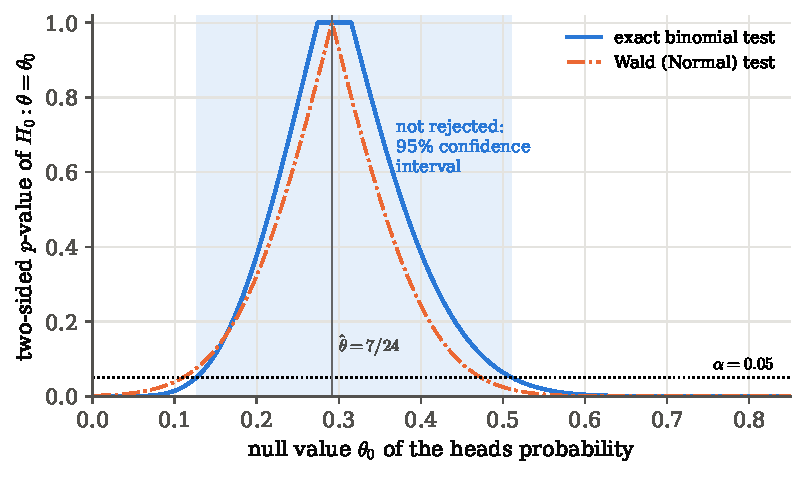
\includegraphics[width=0.85\linewidth]{figures/ch04/pvalue_function.pdf}
\caption{The two-sided p-value of $\theta=\theta_0$ for $7$ successes in $24$
trials, as a function of the hypothesised $\theta_0$. The solid curve uses the
exact binomial tails, the dash-dotted one the Normal (Wald) approximation. Where
a curve stays above the dotted line at $\alpha=0.05$, the null value survives;
the shaded strip is the exact $95\%$ confidence interval. The Wald curve is
symmetric about $\hat\theta$ and shifted to the left of the exact one.}
\label{4b:fig:pvalue-function}
\end{figure}

\paragraph{Two cheaper intervals for the same data.}
The exact interval needs a root finder. Two shortcuts avoid it. The first,
the Normal (Wald) interval, treats the observed fraction $\hat\theta=z/N$ as
Gaussian with mean $\theta$ and estimated standard error
$\widehat{\rm se}=\sqrt{\hat\theta(1-\hat\theta)/N}$. Its coverage is right
only in the large-sample limit \mainref{Thm.~6.16}. To see why, write
$\hat\theta_n$ for the estimate from $n$ trials and suppose
$(\hat\theta_n-\theta)/\widehat{\rm se}$ tends in distribution to
$Z\sim\Normal(0,1)$ (here $Z$ is a standard normal variable, not the count).
Then
\begin{align}
  \Prob_\theta\bigl(\hat\theta_n-z_{\alpha/2}\widehat{\rm se}<\theta<\hat\theta_n+z_{\alpha/2}\widehat{\rm se}\bigr)
  &\eqby{1} \Prob_\theta\Bigl(-z_{\alpha/2}<\frac{\hat\theta_n-\theta}{\widehat{\rm se}}<z_{\alpha/2}\Bigr)
   \notag\\
  &\relby{2}{\longrightarrow} \Prob\bigl(-z_{\alpha/2}<Z<z_{\alpha/2}\bigr)
   \eqby{3} 1-\alpha .
  \label{4b:eq:wald-ci}
\end{align}
\begin{explain}
  \item The same rearrangement of inequalities as in
        \eqref{4b:eq:normal-inversion}, now with $\hat\theta_n$ and
        $\widehat{\rm se}$.
  \item Convergence in distribution: probabilities of intervals converge to
        those of the limit.
  \item The definition of $z_{\alpha/2}$ puts $\alpha/2$ in each tail.
\end{explain}
For the trigger, $\widehat{\rm se}=\FourBKrSe$ and the interval is
$[\FourBKrWaldLo,\FourBKrWaldHi]$. It is symmetric about $\hat\theta$, while
the exact one reaches further up, because a binomial with $\theta$ below one half
has a longer right tail. The second shortcut, from Hoeffding's inequality, gives
a third interval,
$\hat\theta\pm\epsilon_N$ with $\epsilon_N^2=\ln(2/\alpha)/(2N)$, which covers
with probability at least $1-\alpha$ for \emph{every} $N$, not just in the
limit \mainref{Ex.~6.15}. Here $\epsilon_N=\FourBKrHoefEps$ and the interval
is $[\FourBKrHoefLo,\FourBKrHoefHi]$, almost twice as long. That is the price
of a guarantee that uses nothing about the binomial except that each trial is
between $0$ and $1$. So the trade is: the Normal interval is shorter, but its
coverage is only approximately right \mainref{Ex.~6.17}. How far off it is, we
measure in \cref{4b:sec:coverage}.

\paragraph{Example: inverting a likelihood-ratio test.}
Test inversion works with any test, including the likelihood-ratio test.
Casella and Berger take $n$ lifetimes from an exponential distribution with
mean $\lambda$ \srcref{CasellaBerger}{Ex.~9.2.3}. The likelihood is
$\lambda^{-n}e^{-\sum x_i/\lambda}$, it is largest at $\hat\lambda=\sum x_i/n$,
and the ratio of the likelihood at $\lambda_0$ to its maximum is
\begin{align}
  \frac{\lambda_0^{-n}e^{-\sum x_i/\lambda_0}}{\hat\lambda^{-n}e^{-n}}
  &\eqby{1} \Bigl(\frac{\sum x_i}{n\lambda_0}\Bigr)^{n}e^{\,n}\,e^{-\sum x_i/\lambda_0} .
  \label{4b:eq:exp-lrt}
\end{align}
\begin{explain}
  \item Insert $\hat\lambda=\sum x_i/n$ in the denominator, so that
        $e^{-\sum x_i/\hat\lambda}=e^{-n}$, and collect powers.
\end{explain}
The test retains $\lambda_0$ when this ratio is large, above some threshold
$k$. Write $T=\sum x_i/\lambda_0$. Then the ratio is $(T/n)^n e^{n}e^{-T}$, so
the condition is $T^ne^{-T}\ge k^*$, where the constant $n^n/e^n$ has been moved
into the new threshold $k^*=kn^n/e^n$. The function $T^ne^{-T}$ rises and then
falls, so it is above a level exactly on a stretch $b\le T\le a$ whose ends have
equal height, $a^ne^{-a}=b^ne^{-b}$. Solving $b\le\sum x_i/\lambda_0\le a$ for
$\lambda_0$ gives the interval $\sum x_i/a\le\lambda\le\sum x_i/b$.

\emph{Its coverage.} The interval covers the true $\lambda$ exactly when
$T=\sum X_i/\lambda$ lies between $b$ and $a$. Each $X_i/\lambda$ is
exponential with mean one, whatever $\lambda$ is, so $T$ is a sum of $n$
exponentials of mean one, a $\mathrm{Gamma}(n,1)$ variable, with the same
distribution for every $\lambda$. For $n=2$ its density is $te^{-t}$, and
\begin{align}
  \Prob(b\le T\le a)
  &\eqby{1} \int_b^a te^{-t}\,\dd t
   \eqby{2} \bigl[-te^{-t}\bigr]_b^a+\int_b^a e^{-t}\,\dd t
   \eqby{3} e^{-b}(b+1)-e^{-a}(a+1) .
  \label{4b:eq:exp-coverage}
\end{align}
\begin{explain}
  \item The $\mathrm{Gamma}(2,1)$ density.
  \item Integration by parts with $u=t$, $\dd v=e^{-t}\dd t$.
  \item Evaluate both terms and collect.
\end{explain}
Requiring $0.90$ and $a^2e^{-a}=b^2e^{-b}$ at the same time gives $a=5.480$,
$b=0.441$ and a confidence coefficient of $0.90006$. As a check:
$e^{-0.441}\times1.441=0.9272$ and $e^{-5.480}\times6.480=0.0270$, whose
difference is $0.900$; and $5.480^2e^{-5.480}=0.125=0.441^2e^{-0.441}$. The
interval for two lifetimes is $[\sum x_i/5.48,\ \sum x_i/0.441]$, a factor of
twelve wide.

The exponential example worked so smoothly because $T=\sum X_i/\lambda$ has a
distribution that does not depend on $\lambda$. Such a function of data and
parameter is called a \newterm{pivot} \srcref{CasellaBerger}{Def.~9.2.6}.
$(\bar X-\mu)/(\sigma/\sqrt n)$ is a pivot for a Gaussian mean, and
$(\bar X-\mu)/(S/\sqrt n)$, with the sample standard deviation $S$, is a pivot
with a Student $t_{n-1}$ distribution when $\sigma$ is unknown. A pivot gives
an interval whose coverage is the same for every parameter value, and the
coverage can be computed once. Without a pivot, as for the binomial, coverage
depends on $\theta$, and we have to check it everywhere
(\cref{4b:sec:coverage}).

\paragraph{One-sided limits.}
Inverting one-sided tests gives one-sided intervals. To get an \emph{upper}
bound for a Gaussian mean with unknown $\sigma$, test $\mu=\mu_0$ against
$\mu<\mu_0$. The level-$\alpha$ test rejects when
$(\bar x-\mu_0)/(s/\sqrt n)<-t_{n-1,\alpha}$, so it retains when
$\mu_0\le\bar x+t_{n-1,\alpha}s/\sqrt n$, and the survivors form
$(-\infty,\ \bar x+t_{n-1,\alpha}s/\sqrt n]$ \srcref{CasellaBerger}{Ex.~9.2.4}.
The alternative decides the shape: an alternative of \emph{small} values
rejects large $\mu_0$, and what survives is everything below a bound. Upper
limits on signal rates in searches are built this way (\cref{4b:sec:boundary}).

\subsection{Tests and intervals give the same verdict}
\label{4b:sec:duality}

Wasserman states the special case of test inversion that practitioners use
every day \mainref{Thm.~10.10}: the size-$\alpha$ Wald test rejects
$\theta=\theta_0$ exactly when $\theta_0$ lies outside
$\hat\theta\pm z_{\alpha/2}\widehat{\rm se}$. It is \eqref{4b:eq:normal-inversion}
with $\widehat{\rm se}$ in place of $\sigma/\sqrt n$. Checking whether a null
value is inside a $95\%$ interval \emph{is} a test at the $5\%$ level.

The interval carries more information than the verdict, and that answers a
common confusion between statistical and scientific significance
\mainref{p.~155}. \Cref{4b:fig:significance} shows two intervals that both
exclude $\theta_0$, so both tests reject. In the first, the whole interval sits
close to $\theta_0$: the effect is real but tiny, perhaps too small to matter.
In the second, the interval is far away: the effect is large. A p-value alone
cannot tell these apart; the interval can. A $3\times10^{-4}$ shift in a
calibration constant can be ``highly significant'' with enough data and still
irrelevant to every physics result that uses the constant.

\begin{figure}[htbp]
\centering
\begin{tikzpicture}[x=1cm,y=1cm]
  \foreach \yy/\lo/\hi/\lab in {1.3/0.35/1.05/{small effect},0/2.6/4.4/{large effect}}{
    \draw[->,black!60] (-0.6,\yy) -- (5.4,\yy) node[right,font=\small] {$\theta$};
    \draw[bdryred,thick] (0,\yy-0.2) -- (0,\yy+0.2);
    \node[font=\small,bdryred,anchor=north] at (0,\yy-0.22) {$\theta_0$};
    \draw[formblue,line width=2.4pt] (\lo,\yy) -- (\hi,\yy);
    \fill[formblue] ({(\lo+\hi)/2},\yy) circle (2.2pt);
    \node[font=\footnotesize,anchor=south] at ({(\lo+\hi)/2},\yy+0.12) {\lab};
  }
\end{tikzpicture}
\caption{Statistical versus scientific significance. Both $95\%$ intervals
(blue bars, dots at the estimates) exclude the null value $\theta_0$, so both
data sets reject $\Hnull$ at the $5\%$ level. In the top row the effect is
close to $\theta_0$ and may not matter in practice; in the bottom row it is
large. The interval reports the size of the effect; the test only reports that
it is not zero.}
\label{4b:fig:significance}
\end{figure}

\subsection{The interval inherits the test's intentions}
\label{4b:sec:ci-intentions}

The first part of the chapter found that a p-value depends on the stopping
rule: the same $7$ heads in $24$ flips gave different p-values when the
experimenter meant to stop at $N=24$, at $z=7$, or when time ran out. An
interval built from those tests inherits the dependence. Kruschke works out the
$95\%$ intervals for the four intentions \srcref{Kruschke}{pp.~318--321}:
\begin{center}
\begin{tabular}{lc}
\toprule
intention of the experimenter & $95\%$ confidence interval for $\theta$ \\
\midrule
stop after $N=24$ trials & $[0.126,\ 0.511]$ \\
stop after $z=7$ successes & $[0.126,\ 0.484]$ \\
stop when the time is up & $[0.135,\ 0.497]$ \\
test two coins, each with fixed $N$ & $[0.110,\ 0.539]$ \\
\bottomrule
\end{tabular}
\end{center}
The data are identical in all four rows. What differs is the cloud of
experiments that \emph{could} have happened, and a confidence interval, like a
p-value, is a statement about that cloud. For a trigger test this is not
academic. A run stopped ``when the beam went down'' has a random $N$, and
strictly its interval must be computed for that plan. \Cref{4b:sec:credible}
returns to this point: the Bayesian interval depends on the data only through
the likelihood and does not care why the experimenter stopped.

\paragraph{Python.}
The inversion for the trigger is a few lines of
\pyname{code/ch04/11_test_inversion.py}.

\pyfile[firstline=29,lastline=45,label={4b:lst:inversion}]{code/ch04/11_test_inversion.py}{The exact binomial interval by test inversion}

The two functions are the tails in \eqref{4b:eq:clopper}:
\pyname{binom.cdf(z, N, t)} is $\Prob(Z\le z)$ and \pyname{binom.sf(z - 1, N, t)} is
$\Prob(Z\ge z)$ (the survival function is a strict inequality, hence the
$z-1$). The p-value function is twice the smaller tail, capped at one. The
interval ends come from a root finder: \pyname{brentq} solves ``tail $=\alpha/2$''
on the side of $\hat\theta$ where that tail is the one that shrinks. The last
lines check the result against a closed form. Integrating the beta density by
parts $z$ times shows that $\Prob(Z\ge z\given\theta)$ equals the probability that
a $\mathrm{Beta}(z,N-z+1)$ variable is below $\theta$, so $\theta_L$ is a beta
quantile, and similarly for $\theta_U$; the assertion confirms that the root
finder and the identity agree to $10^{-6}$.

\begin{pitfall}[``The parameter is in the interval with probability 95\%'']
After the experiment the interval is two numbers, $[\FourBKrLo,\FourBKrHi]$, and
the efficiency is one number. Either it is inside or it is not; in the
frequentist framework the probability is $0$ or $1$, and we do not know which
\srcref{Cowan}{p.~123}. The $95\%$ belongs to the recipe that produced the two
numbers. Saying ``the efficiency lies in $[0.126, 0.511]$ with probability
$95\%$'' is a statement about $\theta$ given the data, an inference-direction
statement, and it needs a prior (\cref{4b:sec:credible}, \cref{ch:05}).
\end{pitfall}
\section{The Neyman construction: a belt of acceptance regions}
\label{4b:sec:neyman}

A calorimeter measures the energy of a jet. The estimate $\hat\theta$ it
returns is not Gaussian: at low energy the response is skewed, at high energy
it is wider, and the shape of the scatter changes with the true energy
$\theta$. From test beams or simulation we know, for every true $\theta$, the
distribution $g(\hat\theta;\theta)$ of the estimate. We see one number,
$\hat\theta_{\rm obs}$, and want an interval for $\theta$ that covers the true
energy in, say, $68.3\%$ of repeated measurements, whatever that energy is.

Test inversion (\cref{4b:sec:inversion-theorem}) already tells us what to do.
For every $\theta$, choose a set of $\hat\theta$ values that has probability
$1-\alpha$ under $g(\cdot;\theta)$. Then collect the $\theta$ whose set contains
the observation. Drawing all those sets at once on one graph is Neyman's
construction of 1937 \srcref{Cowan}{\S9.2}, \cite{FeldmanCousins1998}. Every
other frequentist interval in this chapter is a special case of it, or a
shortcut to it.

\paragraph{The question in words.}
Given only the family of sampling distributions $g(\hat\theta;\theta)$:
how do we draw a region in the (data, parameter) plane that yields, for any
observed $\hat\theta$, an interval with guaranteed coverage? And how does the
recipe look for the two workhorses, a Gaussian estimate and a Poisson count?

\subsection{The construction, step by step}
\label{4b:sec:belt}

We use the convention of Feldman and Cousins: the measured quantity on the
horizontal axis, the parameter on the vertical axis \cite{FeldmanCousins1998}.

\begin{enumerate}[label=\textbf{Step \arabic*.},leftmargin=*]
  \item \emph{For one hypothetical $\theta$, pick an acceptance interval.}
        Along the horizontal line at height $\theta$, choose
        $[v_\beta(\theta),u_\alpha(\theta)]$ such that the estimate falls above
        $u_\alpha$ with probability $\alpha$ and below $v_\beta$ with
        probability $\beta$ \srcref{Cowan}{(9.1)--(9.2)}:
        \begin{equation}
          \alpha=\int_{u_\alpha(\theta)}^{\infty}g(\hat\theta;\theta)\,\dd\hat\theta,
          \qquad
          \beta=\int_{-\infty}^{v_\beta(\theta)}g(\hat\theta;\theta)\,\dd\hat\theta .
          \label{4b:eq:belt-edges}
        \end{equation}
        \emph{Why legitimate?} We only used $g(\cdot;\theta)$, which we know
        for every $\theta$ by assumption. The data play no role yet.
  \item \emph{Repeat for every $\theta$.} The horizontal intervals sweep out a
        region, the \newterm{confidence belt}, bounded by the curves
        $v_\beta(\theta)$ on the left and $u_\alpha(\theta)$ on the right. For
        every $\theta$, by construction,
        $\Prob\bigl(v_\beta(\theta)\le\hat\theta\le u_\alpha(\theta)\bigr)=1-\alpha-\beta$
        \srcref{Cowan}{(9.3)}.
  \item \emph{Do the experiment, draw a vertical line at $\hat\theta_{\rm
        obs}$.} The confidence interval $[a,b]$ is the set of $\theta$ whose
        horizontal interval is cut by the line.
        \emph{Why legitimate?} This is \eqref{4b:eq:inversion}: the horizontal
        interval at $\theta$ is the acceptance region of a test of $\theta$,
        and the vertical cut collects the values not rejected.
\end{enumerate}

\emph{Why does the result cover?} \Cref{4b:fig:belt} shows it. Suppose the
truth is $\theta_{\rm true}$, a height on the graph that we do not know.
\begin{itemize}[itemsep=1pt,leftmargin=1.2em]
  \item The interval contains $\theta_{\rm true}$ exactly when the vertical
        line at $\hat\theta_{\rm obs}$ cuts the horizontal segment at height
        $\theta_{\rm true}$.
  \item That happens exactly when $\hat\theta_{\rm obs}$ falls inside that
        segment.
  \item By Step~1, the estimate falls inside the segment at the true height
        with probability $1-\alpha-\beta$.
\end{itemize}
So the coverage equals the probability inside the horizontal segment at the
true value. We made that $1-\alpha-\beta$ at every height, so it holds whatever
the truth is.

\begin{figure}[htbp]
\centering
\begin{tikzpicture}[x=1.05cm,y=1.05cm]
  \fill[formblue!10] (-0.6,0) -- (0.9,0) -- (6.9,5) -- (3.4,5) -- cycle;
  \draw[formblue,thick] (-0.6,0) -- (3.4,5);
  \draw[formblue,thick] (0.9,0) -- (6.9,5);
  \draw[->,thick,black!70] (-1,0) -- (7.3,0) node[below left] {estimate $\hat\theta$};
  \draw[->,thick,black!70] (-1,0) -- (-1,5.4) node[above right] {parameter $\theta$};
  \node[formblue,font=\footnotesize,anchor=east] at (2.4,3.75) {$v_\beta(\theta)$};
  \node[formblue,font=\footnotesize,anchor=west] at (5.8,4.05) {$u_\alpha(\theta)$};
  \foreach \t in {0.5,1.5,3.5}{
    \draw[formblue!60,line width=1.3pt] ({0.8*\t-0.6},\t) -- ({1.2*\t+0.9},\t);
  }
  \draw[fibreorange,line width=2.2pt] (1.4,2.5) -- (3.9,2.5);
  \draw[black!40,dashed] (-1,2.5) -- (1.4,2.5);
  \node[anchor=east,font=\small] at (-1,2.5) {$\theta_{\rm true}$};
  \draw[black!60,dashed] (3,0) -- (3,5.2);
  \draw[tangentgreen,line width=2.2pt] (3,1.75) -- (3,4.5);
  \node[anchor=north,font=\small] at (3,0) {$\hat\theta_{\rm obs}$};
  \fill[tangentgreen!70!black] (3,1.75) circle (1.6pt);
  \fill[tangentgreen!70!black] (3,4.5) circle (1.6pt);
  \node[anchor=west,font=\small,tangentgreen!60!black] at (3.08,1.62) {$a$};
  \node[anchor=east,font=\small,tangentgreen!60!black] at (2.92,4.62) {$b$};
\end{tikzpicture}
\caption{A confidence belt. For each hypothetical $\theta$ (vertical axis) the
horizontal segment holds the estimates that are accepted, with probability
$1-\alpha-\beta$; a few are drawn, and the one at the true value is orange. The
vertical line at the observed estimate cuts the belt between $a$ and $b$ (green):
that is the confidence interval. The lower end $a$ comes from the right edge of
the belt, the upper end $b$ from the left edge. The green interval contains
$\theta_{\rm true}$ exactly when the observed estimate lies on the orange
segment.}
\label{4b:fig:belt}
\end{figure}

\begin{workdef}[confidence belt]
For each parameter value $\theta$ an \newterm{acceptance interval}
$[v_\beta(\theta),u_\alpha(\theta)]$ of the estimate, with probability
$1-\alpha-\beta$ under $g(\hat\theta;\theta)$. The union over $\theta$ is the
\newterm{confidence belt}. The interval for an observation is the vertical cut
of the belt at $\hat\theta_{\rm obs}$.
\emph{Operational recipe:} on a grid of $\theta$, compute the acceptance
interval from the known (or simulated) distribution of the estimate; for the
observed value, keep every grid point whose interval contains it.
\end{workdef}

\paragraph{The same thing with inverse functions.}
If the estimator is a good one, both edges increase with $\theta$: a larger
true value gives larger estimates. Then they can be inverted,
$a(\hat\theta)\equiv u_\alpha^{-1}(\hat\theta)$ and
$b(\hat\theta)\equiv v_\beta^{-1}(\hat\theta)$ \srcref{Cowan}{(9.4)}, and the
coverage follows in two lines. Fix the true $\theta$. Then
\begin{align}
  \Prob\bigl(a(\hat\theta)\ge\theta\bigr)
  &\eqby{1} \Prob\bigl(\hat\theta\ge u_\alpha(\theta)\bigr)
   \eqby{2} \alpha ,
  \qquad
  \Prob\bigl(b(\hat\theta)\le\theta\bigr)
   \eqby{3} \Prob\bigl(\hat\theta\le v_\beta(\theta)\bigr)
   \eqby{4} \beta ,
  \notag\\
  \Prob\bigl(a(\hat\theta)<\theta<b(\hat\theta)\bigr)
  &\eqby{5} 1-\alpha-\beta .
  \label{4b:eq:belt-coverage}
\end{align}
\begin{explain}
  \item $u_\alpha$ is increasing, so applying it to both sides of
        $a(\hat\theta)\ge\theta$ preserves the inequality, and
        $u_\alpha(a(\hat\theta))=\hat\theta$ by the definition of the inverse.
  \item The definition of $u_\alpha$ in \eqref{4b:eq:belt-edges}.
  \item The same step for $v_\beta$ and $b$.
  \item The definition of $v_\beta$.
  \item The two ``miss'' events cannot happen together, because $a<b$ (the
        right edge of the belt lies to the right of the left edge), so the
        probability of a hit is one minus the sum of the two.
\end{explain}
The random quantities are $a$ and $b$: they depend on $\hat\theta$. Repeated
experiments give different intervals, and a fraction $1-\alpha-\beta$ of them
contain the fixed $\theta$ \srcref{Cowan}{p.~121}.

In practice we find $a$ and $b$ without drawing the belt. By the definition of
the inverses, $u_\alpha(a)=\hat\theta_{\rm obs}$ and $v_\beta(b)=\hat\theta_{\rm
obs}$. Putting these into \eqref{4b:eq:belt-edges}, at $\theta=a$ for the first
integral and $\theta=b$ for the second, gives \srcref{Cowan}{(9.9)}
\begin{equation}
  \alpha=\int_{\hat\theta_{\rm obs}}^{\infty}g(\hat\theta;a)\,\dd\hat\theta,
  \qquad
  \beta=\int_{-\infty}^{\hat\theta_{\rm obs}}g(\hat\theta;b)\,\dd\hat\theta .
  \label{4b:eq:belt-ends}
\end{equation}
In words: the lower end $a$ is the parameter value for which an estimate as
large as the one observed, or larger, would occur with probability $\alpha$;
the upper end $b$ is the value for which an estimate this small or smaller
would occur with probability $\beta$. Each end is a one-sided test with
p-value exactly $\alpha$ (or $\beta$). Beware of the names here. The p-value of
the test of $\theta=a$ is $\alpha$, a small number. The confidence level of the
limit $\theta\ge a$ is $1-\alpha$, a large one. To keep them apart we say
``confidence level'' only for the coverage of an interval and ``p-value'' only
for tests \srcref{Cowan}{pp.~122--123}.

\paragraph{Central and one-sided.}
The recipe leaves one choice free: how to split the excluded probability
between the two sides. If the total excluded probability is $\gamma$, then
$\alpha=\beta=\gamma/2$ gives a \newterm{central} interval of level
$1-\gamma$. $\beta=0$ gives a lower limit, $\alpha=0$ an upper limit. A
central interval has equal probabilities of missing on either side; it need not
be symmetric about the estimate. And the choice must be made \emph{before}
looking at the data. \Cref{4b:sec:boundary} shows what goes wrong when the data
decide it.

\subsection{Gaussian estimate: the error bar is a 68.3\% interval}
\label{4b:sec:belt-gauss}

When $g(\hat\theta;\theta)$ is Gaussian with mean $\theta$ and known standard
deviation $\sigma_{\hat\theta}$, the cumulative distribution is
$G(\hat\theta;\theta)=\Phi\bigl((\hat\theta-\theta)/\sigma_{\hat\theta}\bigr)$
\srcref{Cowan}{(9.10)}. Then \eqref{4b:eq:belt-ends} can be solved in closed
form:
\begin{align}
  \alpha
  &\eqby{1} 1-\Phi\Bigl(\frac{\hat\theta_{\rm obs}-a}{\sigma_{\hat\theta}}\Bigr)
  \ \Longrightarrow\
  a \eqby{2} \hat\theta_{\rm obs}-\sigma_{\hat\theta}\,\Phi^{-1}(1-\alpha),
  \notag\\
  \beta
  &\eqby{3} \Phi\Bigl(\frac{\hat\theta_{\rm obs}-b}{\sigma_{\hat\theta}}\Bigr)
  \ \Longrightarrow\
  b \eqby{4} \hat\theta_{\rm obs}-\sigma_{\hat\theta}\,\Phi^{-1}(\beta)
    \eqby{5} \hat\theta_{\rm obs}+\sigma_{\hat\theta}\,\Phi^{-1}(1-\beta).
  \label{4b:eq:gauss-ends}
\end{align}
\begin{explain}
  \item The upper tail beyond $\hat\theta_{\rm obs}$ of a Gaussian centred on
        $a$.
  \item Solve: $\Phi\bigl((\hat\theta_{\rm obs}-a)/\sigma\bigr)=1-\alpha$, apply
        $\Phi^{-1}$ and rearrange.
  \item The lower tail below $\hat\theta_{\rm obs}$ of a Gaussian centred on $b$.
  \item Apply $\Phi^{-1}$ and rearrange.
  \item Symmetry of the Gaussian: $\Phi^{-1}(\beta)=-\Phi^{-1}(1-\beta)$.
\end{explain}
With $\alpha=\beta=0.1587$, $\Phi^{-1}(1-\alpha)=1$ and the $68.3\%$ central
interval is $\hat\theta_{\rm obs}\pm\sigma_{\hat\theta}$ \srcref{Cowan}{(9.13)}.
This is the precise sense in which a ``one-sigma error bar'' is a confidence
interval. The standard quantiles, which every physicist ends up knowing by
heart \srcref{Cowan}{Tables~9.1--9.2}:
\begin{center}
\begin{tabular}{ccc@{\qquad}ccc}
\toprule
\multicolumn{3}{c}{central, $1-\gamma$} & \multicolumn{3}{c}{one-sided, $1-\alpha$}\\
\cmidrule(r){1-3}\cmidrule(l){4-6}
$\Phi^{-1}(1-\gamma/2)$ & $1-\gamma$ & & $\Phi^{-1}(1-\alpha)$ & $1-\alpha$ & \\
\midrule
$1$ & $0.6827$ & & $1$ & $0.8413$ &\\
$2$ & $0.9544$ & & $2$ & $0.9772$ &\\
$3$ & $0.9973$ & & $3$ & $0.9987$ &\\
$1.645$ & $0.90$ & & $1.282$ & $0.90$ &\\
$1.960$ & $0.95$ & & $1.645$ & $0.95$ &\\
$2.576$ & $0.99$ & & $2.326$ & $0.99$ &\\
\bottomrule
\end{tabular}
\end{center}
The number $1.645$ appears twice: it is the central $90\%$ quantile and the
one-sided $95\%$ one. This coincidence matters when a parameter sits at a
physical boundary (\cref{4b:sec:boundary}).

Physicists use the same convention, the $68.3\%$ central interval, for error
bars even when $g$ is not Gaussian. The interval is then no longer symmetric,
and the result is quoted as $\hat\theta^{+d}_{-c}$, meaning $a=\hat\theta-c$ and
$b=\hat\theta+d$. For example, $5.79^{+0.32}_{-0.25}$ means: the recipe that
produced $[5.54,6.11]$ covers the true value in $68.3\%$ of repeated
experiments, with equal chances of missing high and low. It does not mean that $\theta$ lies in $[5.54,6.11]$ with
probability $68.3\%$ \srcref{Cowan}{p.~123}. When $\sigma_{\hat\theta}$ is itself
estimated from the data, the pivot becomes Student's $t$; for large samples the
Gaussian recipe with the estimated $\hat\sigma$ is fine, for small ones it is
not, and \cref{4b:sec:coverage} measures by how much.

\subsection{Poisson counts: a belt with steps}
\label{4b:sec:belt-poisson}

A count $n$ of rare events is Poisson with mean $\nu$, and the estimate is
$\hat\nu=n$ \srcref{Cowan}{(9.14)}. \emph{What changes:} the estimate now takes
only integer values. So \eqref{4b:eq:belt-edges} cannot be satisfied exactly.
The tail probability beyond an integer changes in jumps from one integer to the
next, and for a given $\alpha$ there is usually no integer $u_\alpha(\nu)$ whose
tail is exactly $\alpha$. \emph{The fix:} keep the end conditions
\eqref{4b:eq:belt-ends}, and count the observed value as part of each tail
\srcref{Cowan}{(9.15)--(9.16)}:
\begin{equation}
  \alpha=\Prob(n\ge n_{\rm obs};a)=1-\sum_{n=0}^{n_{\rm obs}-1}\frac{a^n}{n!}e^{-a},
  \qquad
  \beta=\Prob(n\le n_{\rm obs};b)=\sum_{n=0}^{n_{\rm obs}}\frac{b^n}{n!}e^{-b}.
  \label{4b:eq:poisson-ends}
\end{equation}
These can be solved numerically. There is also a closed form, because the
Poisson cumulative sum is a $\chi^2$ tail \srcref{Cowan}{(9.17)}:
\begin{equation}
  \sum_{n=0}^{k}\frac{\nu^n}{n!}e^{-\nu}
  =\int_{2\nu}^{\infty}f_{\chi^2}\bigl(z;\,2(k+1)\bigr)\,\dd z ,
  \qquad
  f_{\chi^2}(z;m)=\frac{z^{m/2-1}e^{-z/2}}{2^{m/2}\,\Gamma(m/2)} .
  \label{4b:eq:poisson-chi2}
\end{equation}
To prove the identity, we show that the two sides start at the same value and
change at the same rate. Call the left side $F(\nu)$ and the right side
$H(\nu)$. Both equal one at $\nu=0$: on the left only the $n=0$ term survives,
and on the right the whole $\chi^2$ density is integrated. Their derivatives
are
\begin{align}
  F'(\nu)
  &\eqby{1} \sum_{n=0}^{k}\Bigl(\frac{n\nu^{n-1}}{n!}-\frac{\nu^n}{n!}\Bigr)e^{-\nu}
   \eqby{2} \sum_{n=1}^{k}\frac{\nu^{n-1}}{(n-1)!}e^{-\nu}-\sum_{n=0}^{k}\frac{\nu^{n}}{n!}e^{-\nu}
   \eqby{3} -\frac{\nu^{k}}{k!}e^{-\nu},
  \notag\\
  H'(\nu)
  &\eqby{4} -2\,f_{\chi^2}\bigl(2\nu;\,2k+2\bigr)
   \eqby{5} -2\,\frac{(2\nu)^{k}e^{-\nu}}{2^{k+1}\,k!}
   \eqby{6} -\frac{\nu^{k}}{k!}e^{-\nu}.
  \label{4b:eq:poisson-chi2-proof}
\end{align}
\begin{explain}
  \item Product rule on $\nu^ne^{-\nu}$.
  \item Cancel $n$ against $n!$ in the first sum; its $n=0$ term is zero.
  \item Shift $n-1\to n$ in the first sum: it becomes the second sum without
        its last term, so everything cancels except $-\nu^ke^{-\nu}/k!$.
  \item Fundamental theorem of calculus, with the lower limit $2\nu$ whose
        derivative is $2$.
  \item Insert the density with $m=2k+2$: $z^{m/2-1}=(2\nu)^k$,
        $e^{-z/2}=e^{-\nu}$, $2^{m/2}=2^{k+1}$, $\Gamma(k+1)=k!$.
  \item Simplify $2\cdot2^k/2^{k+1}=1$.
\end{explain}
The two functions are equal at $\nu=0$ and have equal derivatives everywhere,
so they are equal for every $\nu$. Applying the identity to the two conditions
in \eqref{4b:eq:poisson-ends} (with $k=n_{\rm obs}-1$ for $a$ and
$k=n_{\rm obs}$ for $b$) turns each into a $\chi^2$ probability up to $2a$ or beyond $2b$, so the
limits are quantiles of $\chi^2$ distributions \srcref{Cowan}{(9.18)}:
\begin{equation}
  a=\tfrac12F^{-1}_{\chi^2}(\alpha;\,2n_{\rm obs}),
  \qquad
  b=\tfrac12F^{-1}_{\chi^2}(1-\beta;\,2(n_{\rm obs}+1)) ,
  \label{4b:eq:garwood}
\end{equation}
where $F^{-1}_{\chi^2}(p;m)$ is the $p$ quantile with $m$ degrees of freedom.
These are Garwood's intervals of 1936 \srcref{CasellaBerger}{Ex.~9.2.15}. For
$n$ independent Poisson observations of rate $\lambda$ the sum is
Poisson$(n\lambda)$, and the interval for $\lambda$ is \eqref{4b:eq:garwood}
divided by $n$; with $n=10$ observations summing to $6$, the $90\%$ interval is
$[\FourBCBlo,\ \FourBCBhi]$.\footnote{Casella and Berger print $0.262$ for the
lower end; $F^{-1}_{\chi^2}(0.05;12)/20=5.226/20=0.2613$.}

\paragraph{Example: zero events.}
If nothing is seen, $n_{\rm obs}=0$, there is no lower limit and the upper limit
solves $\beta=e^{-b}$, so $b=-\ln\beta$ \srcref{Cowan}{(9.20)}. At $95\%$,
$b=-\ln0.05=\FourBUpNinetyFiveZero\approx3$: if the mean were $3$, seeing
nothing would happen $5\%$ of the time. This ``rule of three'' is how a search
that sees no candidate events quotes its sensitivity. At $90\%$ it is
$\FourBUpNinetyZero$.

\paragraph{Example: the $90\%$ table.}
Script \pyname{code/ch04/12_neyman_poisson_belt.py} builds the belt by brute
force (for each $\nu$ on a grid, keep the counts whose two tails both exceed
$5\%$), reads off the intervals, and checks them against \eqref{4b:eq:garwood}:
\begin{center}
\small
\begin{tabular}{c*{11}{c}}
\toprule
$n_{\rm obs}$ & 0 & 1 & 2 & 3 & 4 & 5 & 6 & 7 & 8 & 9 & 10\\
\midrule
$a$ & $\FourBBeltLoZero$ & $\FourBBeltLoOne$ & $\FourBBeltLoTwo$ & $\FourBBeltLoThree$ & $\FourBBeltLoFour$ & $\FourBBeltLoFive$ & $\FourBBeltLoSix$ & $\FourBBeltLoSeven$ & $\FourBBeltLoEight$ & $\FourBBeltLoNine$ & $\FourBBeltLoTen$\\
$b$ & $\FourBBeltHiZero$ & $\FourBBeltHiOne$ & $\FourBBeltHiTwo$ & $\FourBBeltHiThree$ & $\FourBBeltHiFour$ & $\FourBBeltHiFive$ & $\FourBBeltHiSix$ & $\FourBBeltHiSeven$ & $\FourBBeltHiEight$ & $\FourBBeltHiNine$ & $\FourBBeltHiTen$\\
\bottomrule
\end{tabular}
\end{center}
These are the $\alpha=0.05$ and $\beta=0.05$ columns of Cowan's Table~9.3. The
belt is in \cref{4b:fig:poisson-belt}. Two features distinguish it from the
Gaussian one. The edges are staircases, because the acceptance set at each
$\nu$ is a set of integers. And the probability inside each horizontal set is
not $0.90$ but somewhere between $\FourBBeltMinAcc$ and $\FourBBeltMaxAcc$,
depending on $\nu$: adding the observed count to each tail makes each tail at
most $5\%$, so the interval covers at least $90\%$
\srcref{Cowan}{(9.19)}. Discreteness buys safety at the price of intervals that
are longer than they need to be for most $\nu$; \cref{4b:sec:coverage} maps the
over-coverage exactly.

\begin{figure}[htbp]
\centering
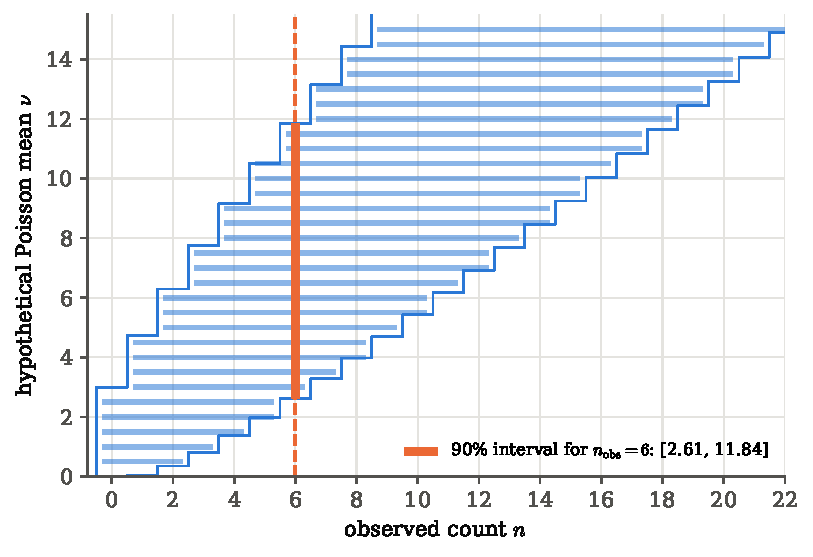
\includegraphics[width=0.8\linewidth]{figures/ch04/poisson_belt.pdf}
\caption{The $90\%$ central confidence belt for a Poisson mean, built by brute
force. Each horizontal bar is the set of counts accepted at one hypothetical
mean $\nu$ (bars drawn every $0.5$); the thin staircases are the edges of the
belt on the fine grid. The dashed vertical line at $n=6$ cuts the belt between
the two ends of the orange bar, the $90\%$ interval for six observed events.}
\label{4b:fig:poisson-belt}
\end{figure}

\paragraph{Python.}
The heart of the brute-force construction:

\pyfile[firstline=28,lastline=46,label={4b:lst:belt}]{code/ch04/12_neyman_poisson_belt.py}{The Poisson belt and its inversion}

\pyname{cdf} and \pyname{sf} are matrices, one row per hypothetical $\nu$ and
one column per count, holding $\Prob(N\le n)$ and $\Prob(N\ge n)$. The boolean
matrix \pyname{keep} marks the counts whose two tails are both larger than
$5\%$: each row is one horizontal acceptance set. Inverting is then a vertical
read: \pyname{interval_from_belt} collects every $\nu$ whose row contains the
observed count. The script then asserts that the brute-force interval equals
Garwood's formula to within the grid spacing, for $n_{\rm obs}=0,\dots,10$.

\subsection{When the estimate is not Gaussian: transform first}
\label{4b:sec:fisher-z}

For a non-Gaussian estimator we can always build the full belt. Sometimes a
change of variables makes that unnecessary. The textbook case is the
correlation coefficient $r$ of $n$ pairs from a two-dimensional Gaussian
\srcref{Cowan}{\S9.5}. Its distribution is skewed, the more so the closer the
true $\rho$ is to $\pm1$, and it is Gaussian only for very large $n$ (Cowan
quotes $n\gtrsim500$).

The trouble is that the spread of $r$ depends on the unknown $\rho$. Fisher's
idea is to transform $r$ so that it does not: a
\newterm{variance-stabilising transformation} \unpack{a function $g$ chosen so
that the variance of $g(r)$ no longer depends on $\rho$}. The variance of $r$
is approximately $(1-\rho^2)^2/n$ \srcref{Cowan}{(5.17)}. The delta method of
\cref{ch:03} (a smooth function of an estimate has variance $g'^2$ times the
estimate's variance) gives $\Var g(r)\approx g'(\rho)^2(1-\rho^2)^2/n$. This is
independent of $\rho$ if $g'(\rho)=1/(1-\rho^2)$:
\begin{align}
  g(\rho)
  &\eqby{1} \int\frac{\dd\rho}{1-\rho^2}
   \eqby{2} \frac12\int\Bigl(\frac1{1+\rho}+\frac1{1-\rho}\Bigr)\dd\rho
   \eqby{3} \frac12\ln\frac{1+\rho}{1-\rho}
   \eqby{4} \tanh^{-1}\rho .
  \label{4b:eq:fisher-z}
\end{align}
\begin{explain}
  \item Integrate the required derivative.
  \item Partial fractions: $1/(1-\rho^2)=\tfrac12[1/(1+\rho)+1/(1-\rho)]$.
  \item $\int\dd\rho/(1\pm\rho)=\pm\ln(1\pm\rho)$; choose the constant so that
        $g(0)=0$.
  \item The standard form of the inverse hyperbolic tangent.
\end{explain}
So $z=\tanh^{-1}r$ has variance close to $1/n$; a finer calculation gives
$1/(n-3)$ \srcref{Cowan}{(9.22)--(9.25)}, and $z$ is close to Gaussian much
sooner than $r$. The recipe: transform, build the Gaussian interval for
$\zeta=\tanh^{-1}\rho$, transform the ends back with $\tanh$.

\paragraph{Example: $r=0.5$ from $20$ pairs.}
The point first: the naive Gaussian interval claims a correlation, and the
transformed one does not. \emph{Naive.} The naive error
$\hat\sigma_r=(1-r^2)/\sqrt n=\FourBFzSigR$ makes $r$ look like a three-sigma
effect, and the naive $99\%$ interval $[\FourBFzNaiveLo,\FourBFzNaiveHi]$
excludes zero. \emph{Transformed.} Now $z=\tanh^{-1}0.5=\FourBFzZ$ and
$\sigma_z=1/\sqrt{n-3}=1/\sqrt{17}=\FourBFzSigZ$. The $99\%$ interval for
$\zeta$ is $[\FourBFzZetaLo,\FourBFzZetaHi]$, and applying $\tanh$ to its ends
gives $[\FourBFzRhoLo,\FourBFzRhoHi]$ for $\rho$: zero is inside
\srcref{Cowan}{p.~130}. The evidence for a correlation is much weaker than the
naive error suggests. Under
$\rho=0$ the naive Gaussian gives a one-sided probability of
$\FourBFzPnaive\%$ for $r\ge0.5$, the $z$ transformation gives
$\FourBFzPfisher\%$, and the exact calculation (under $\rho=0$,
$r\sqrt{n-2}/\sqrt{1-r^2}$ is Student $t$ with $n-2$ degrees of freedom, here
$t=\FourBFzT$) gives $\FourBFzPexact\%$.\footnote{Cowan quotes $2.3\%$ for
the $z$ transformation. We find $\FourBFzPfisher\%$ for the one-sided tail,
in agreement with the exact $t$ calculation; $2.3\%$ is close to the two-sided
value.} Which interval should we trust? A simulation of $10^5$ samples of $20$
pairs settles it. At $\rho=0.5$ the naive $99\%$ interval covers only
$\FourBFzCovNaiveFive$ of the time, the Fisher interval $\FourBFzCovFisherFive$;
at $\rho=0.8$, $\FourBFzCovNaiveEight$ against $\FourBFzCovFisherEight$.

\subsection{Intervals from the likelihood function}
\label{4b:sec:likelihood-interval}

The most widely used interval in physics needs no belt at all. In the large
sample limit, the maximum-likelihood estimator is Gaussian around the true
value with standard deviation $\sigma_{\hat\theta}$, and the likelihood itself
becomes a Gaussian function of $\theta$ around $\hat\theta$ with the same
width \srcref{Cowan}{(9.26)--(9.27)}; the equality of the two widths is the
Cram\'er--Rao bound becoming an equality (\cref{ch:03}). Then
\begin{align}
  \ln\Like(\hat\theta\pm N\sigma_{\hat\theta})
  &\eqby{1} \ln\Like_{\max}-\frac{(N\sigma_{\hat\theta})^2}{2\sigma_{\hat\theta}^2}
   \eqby{2} \ln\Like_{\max}-\frac{N^2}{2} .
  \label{4b:eq:dlnl}
\end{align}
\begin{explain}
  \item $\ln\Like(\theta)=\ln\Like_{\max}-(\theta-\hat\theta)^2/2\sigma_{\hat\theta}^2$
        for a Gaussian likelihood, evaluated at $\theta-\hat\theta=\pm N\sigma_{\hat\theta}$.
  \item Cancel $\sigma_{\hat\theta}^2$.
\end{explain}
So the $68.3\%$ interval is where $\ln\Like$ has dropped by $1/2$ from its
maximum, the $95.4\%$ interval where it has dropped by $2$, and in a
least-squares fit, where $\ln\Like=-\chi^2/2$, where $\chi^2$ has risen by $N^2$
\srcref{Cowan}{(9.28)--(9.30)}:
\begin{equation}
  \ln\Like\bigl(\hat\theta^{+d}_{-c}\bigr)=\ln\Like_{\max}-\frac{N^2}{2},
  \qquad
  \chi^2\bigl(\hat\theta^{+d}_{-c}\bigr)=\chi^2_{\min}+N^2 .
  \label{4b:eq:likelihood-interval}
\end{equation}
This prescription is used, and works well, even when $\ln\Like$ is not a
parabola. \emph{Why?} The reason is that the likelihood does not care how we
label the parameter. Suppose some monotone reparametrisation $\eta=h(\theta)$
makes the likelihood Gaussian in $\eta$. The likelihood is a function on parameter space, and its \emph{values}
do not change when we relabel the points: $\Like$ at the point called $\theta$
equals $\Like$ at the same point called $\eta=h(\theta)$. So the points where
$\ln\Like$ has dropped by $1/2$ are the same points in either labelling. In the
$\eta$ labelling they bound an exact $68.3\%$ interval; mapped back, they bound
an asymmetric interval in $\theta$ with the same coverage. So the recipe uses
the good parametrisation without our having to find it. But it is only as good
as the assumption that such an $h$ exists, and that is guaranteed only for
large samples. That is why the result is called a \emph{likelihood interval}:
it approximates the confidence interval, and is not one exactly
\srcref{Cowan}{p.~131}.

\paragraph{Example: five lifetimes.}
Take $n$ decay times $t_i$ from an exponential with mean $\tau$. With
$\hat\tau=\bar t$ and $u=\hat\tau/\tau$,
\begin{align}
  \ln\Like(\tau)-\ln\Like_{\max}
  &\eqby{1} \Bigl(-n\ln\tau-\frac{n\hat\tau}{\tau}\Bigr)-\bigl(-n\ln\hat\tau-n\bigr)
   \eqby{2} n\Bigl(\ln\frac{\hat\tau}{\tau}-\frac{\hat\tau}{\tau}+1\Bigr)
   \eqby{3} n\,(\ln u-u+1) .
  \label{4b:eq:exp-dlnl}
\end{align}
\begin{explain}
  \item $\ln\Like=\sum_i\ln(\tau^{-1}e^{-t_i/\tau})=-n\ln\tau-\sum_it_i/\tau$, and
        $\sum_it_i=n\hat\tau$; at the maximum $\tau=\hat\tau$ the second term
        is $-n$.
  \item Collect the logarithms.
  \item Definition of $u$.
\end{explain}
The drop depends on the data only through $u$, so the two roots of
$n(\ln u-u+1)=-\tfrac12$ are fixed numbers for each $n$: for $n=5$,
$u=\FourBLiUlo$ and $u=\FourBLiUhi$. The likelihood interval is
$[\hat\tau/\FourBLiUhi,\ \hat\tau/\FourBLiUlo]$ for \emph{every} sample of five.
For the sample simulated in \pyname{code/ch04/14_likelihood_intervals.py} with
true $\tau=1$, $\hat\tau=\FourBLiTauHat$ and the interval is
$[\FourBLiLo,\FourBLiHi]$, that is
$\hat\tau=\FourBLiTauHat^{+\FourBLiPlus}_{-\FourBLiMinus}$
(\cref{4b:fig:likelihood-interval}, left). Cowan's own sample gives
$0.85^{+0.52}_{-0.30}$ \srcref{Cowan}{Fig.~9.6}, the same ratios
$1.61$ and $0.65$ to $\hat\tau$, as the invariance predicts.

Because $u=\hat\tau/\tau$ is a pivot (it is a mean of five exponentials of
mean one, a $\mathrm{Gamma}(5,1/5)$ variable, whatever $\tau$ is), the coverage
of the likelihood interval can be computed exactly: it is
$\Prob(\FourBLiUlo\le U\le\FourBLiUhi)=\FourBLiCovFive$, against a nominal
$0.683$; a Monte Carlo of $2\times10^5$ experiments gives $\FourBLiCovFiveMC$.
The exact central interval for our sample, from the pivot
$2n\hat\tau/\tau\sim\chi^2_{2n}$, is $[\FourBLiExLo,\FourBLiExHi]$. The symmetric
interval $\hat\tau\pm\hat\tau/\sqrt n$ happens to have about the right total
coverage at $n=5$ ($\FourBSymCovFive$), but it distributes its misses badly: it
lies entirely below the truth in $\FourBSymMissBelow$ of experiments and entirely
above it in $\FourBSymMissAbove$, where a central interval would have $0.159$ on
each side. The likelihood interval splits them as $\FourBLiMissBelow$ and
$\FourBLiMissAbove$. \Cref{4b:fig:likelihood-interval} (right) shows how both
approach the nominal coverage as $n$ grows. With $n=50$ Cowan's symmetric
$1.06\pm0.15$ is fine; with $n=5$ the asymmetric likelihood interval is the
honest summary.

\begin{figure}[htbp]
\centering
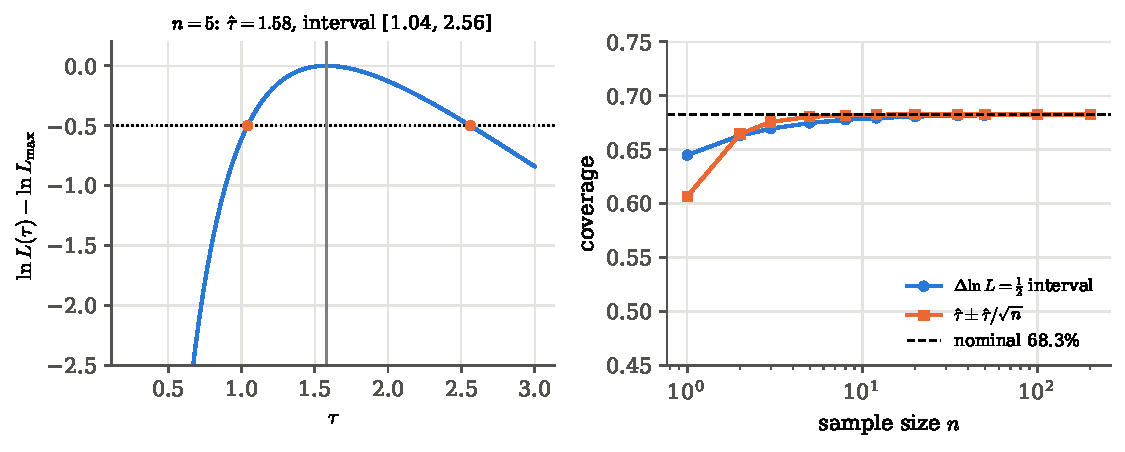
\includegraphics[width=\linewidth]{figures/ch04/likelihood_interval.pdf}
\caption{Left: the log-likelihood of five simulated decay times, relative to its
maximum, as a function of the mean lifetime $\tau$. It is not a parabola: it
falls steeply towards small $\tau$ and slowly towards large $\tau$. The dotted
line is the drop by $1/2$; its two crossings (orange) are the ends of the
likelihood interval. Right: the exact coverage of the $\Delta\ln\Like=\tfrac12$
interval and of the symmetric $\hat\tau\pm\hat\tau/\sqrt n$, as a function of
the sample size; both approach $68.3\%$.}
\label{4b:fig:likelihood-interval}
\end{figure}

\subsection{Several parameters: confidence regions}
\label{4b:sec:regions}

With $m$ parameters $\params=(\theta_1,\dots,\theta_m)$, the large-sample
estimators are jointly Gaussian with covariance $\Cmat$, and the likelihood is a
Gaussian function of $\params$ with the same $\Cmat$
\srcref{Cowan}{(9.31)--(9.33)}. Both are governed by the quadratic form
\begin{equation}
  Q(\hat\params,\params)=(\hat\params-\params)\T\Cmat^{-1}(\hat\params-\params),
  \label{4b:eq:Q}
\end{equation}
which is symmetric in its two arguments. The argument for a confidence region
takes three steps.
\begin{itemize}[itemsep=1pt,leftmargin=1.2em]
  \item \emph{Two readings of one form.} As a function of the estimate at fixed
        truth, the level sets of $Q$ are the ellipses of equal sampling
        density. As a function of the parameters at fixed estimate, they are
        the contours of equal likelihood.
  \item \emph{Its distribution.} At the true $\params$, $Q$ has a $\chi^2_m$
        distribution (\cref{ch:02}): whitening the Gaussian vector turns $Q$
        into a sum of $m$ squared independent standard normals. So
        $\Prob(Q\le Q_\gamma)=1-\gamma$ when
        $Q_\gamma=F^{-1}_{\chi^2}(1-\gamma;m)$, the $1-\gamma$ quantile.
  \item \emph{The symmetry.} ``The estimate is within $Q_\gamma$ of the
        truth'' and ``the truth is within $Q_\gamma$ of the estimate'' are the
        same event.
\end{itemize}
So the region $\{\params:Q(\hat\params,\params)\le Q_\gamma\}$ contains the
truth with probability $1-\gamma$: it is a $1-\gamma$ confidence region. In
practice it is found as the contour \srcref{Cowan}{(9.34)--(9.37)}
\begin{equation}
  \ln\Like(\params)=\ln\Like_{\max}-\frac{Q_\gamma}{2}
  \qquad\text{or}\qquad
  \chi^2(\params)=\chi^2_{\min}+Q_\gamma .
  \label{4b:eq:region}
\end{equation}
The thresholds grow with the number of parameters
\srcref{Cowan}{Tables~9.4--9.5}:
\begin{center}
\begin{tabular}{lccccc}
\toprule
$1-\gamma$ & $m=1$ & $m=2$ & $m=3$ & $m=4$ & $m=5$\\
\midrule
$0.683$ & $1.00$ & $2.30$ & $3.53$ & $4.72$ & $5.89$\\
$0.90$ & $2.71$ & $4.61$ & $6.25$ & $7.78$ & $9.24$\\
$0.95$ & $3.84$ & $5.99$ & $7.82$ & $9.49$ & $11.1$\\
$0.99$ & $6.63$ & $9.21$ & $11.3$ & $13.3$ & $15.1$\\
\bottomrule
\end{tabular}
\end{center}
For $m=1$, $Q_\gamma=N^2$ and the recipe is \eqref{4b:eq:likelihood-interval}.
For $m=2$ the familiar threshold no longer works. The $\Delta\chi^2=1$ contour,
which many plots label ``$1\sigma$'', contains the truth only $39.3\%$ of the
time; the $68.3\%$ region needs $\Delta\chi^2=2.30$. \Cref{4b:fig:ellipse} checks this with a straight-line fit to
ten points, repeated $2\times10^5$ times: the truth falls inside the
$\Delta\chi^2=1$ ellipse in $\FourBElCovOne$ of the experiments and inside the
$\Delta\chi^2=\FourBElQ$ ellipse in $\FourBElCovTwoThirty$. The interval for the
slope \emph{alone}, $\hat\theta_2\pm\sqrt{C_{22}}$, still covers $\FourBElCovSlope$:
a one-parameter question keeps its one-parameter threshold. This is how
cosmological constraints are drawn: the $68\%$ and $95\%$ contours in a plane
of two parameters, and one-dimensional intervals from the marginal or profile
of each (\cref{ch:09,ch:10}).

\begin{figure}[htbp]
\centering
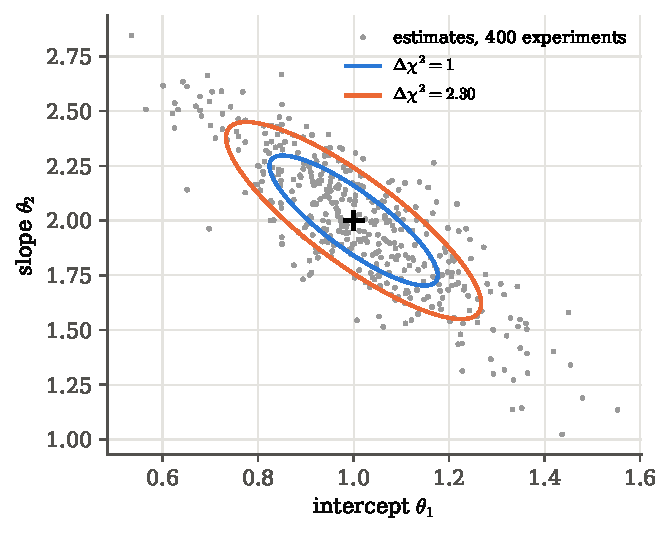
\includegraphics[width=0.6\linewidth]{figures/ch04/ellipse_coverage.pdf}
\caption{Two-parameter confidence regions for a straight-line fit. Grey dots:
the fitted (intercept, slope) from $400$ simulated experiments with the same
true line (cross). The negative tilt is the correlation of the two estimates
(correlation coefficient $\FourBElRho$). The inner ellipse, $\Delta\chi^2=1$,
holds about $39\%$ of the dots, the outer, $\Delta\chi^2=2.30$, about $68\%$.
The same ellipses drawn around any one estimate are its confidence regions.}
\label{4b:fig:ellipse}
\end{figure}

As in one dimension, the region is random and the parameters are fixed
\srcref{Cowan}{p.~135}. And as in one dimension, the $\chi^2_m$ calibration is
only asymptotic. For strongly non-Gaussian likelihoods the coverage of
\eqref{4b:eq:region} must be checked by simulation, as in
\cref{4b:sec:coverage}.
\section{Coverage is a property of the procedure}
\label{4b:sec:coverage}

A hundred groups around the world measure the same Gaussian mean, each with
$n=\FourBLadderN$ readings of known resolution, and each quotes the $95\%$
interval $\bar x\pm1.96\,\sigma/\sqrt n$. \Cref{4b:fig:ladder} shows what
happens in a simulation where we know the truth. The intervals jump up and
down with the data; the true value, the dashed line, stays put; and
$\FourBLadderMiss$ of the hundred intervals miss it. None of the hundred groups
can tell from its own interval whether it is one of the unlucky ones. The
$95\%$ is a property of the whole ladder, not of any rung.

\begin{figure}[htbp]
\centering
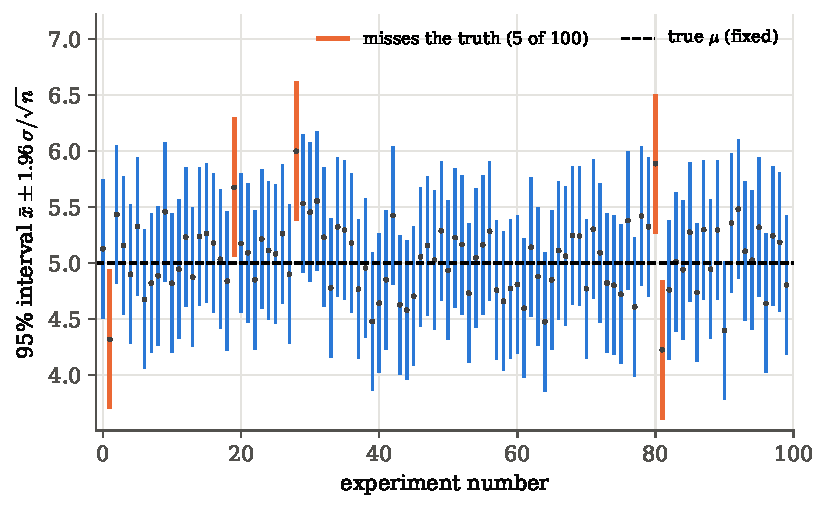
\includegraphics[width=0.85\linewidth]{figures/ch04/coverage_ladder.pdf}
\caption{A hundred simulated experiments, each quoting a $95\%$ interval for the
same Gaussian mean. The vertical bars are the intervals, the dots the sample
means, the dashed line the true value. The intervals move from experiment to
experiment; the truth does not. The orange bars are the intervals that miss it.}
\label{4b:fig:ladder}
\end{figure}

A confidence level is a promise about a \emph{recipe}: apply it to data
generated with any $\theta$, and it will contain that $\theta$ with the stated
probability. We can check by simulation whether a recipe keeps the promise. The
check finds three kinds of fault: recipes that cover less often than they
claim, recipes that cover more often than needed and so are too wide, and,
less obviously, recipes that are right on average but wrong in situations we
can recognise from the data.

\paragraph{The question in words.}
\begin{enumerate}[label=\arabic*.]
  \item For a given recipe, how does the coverage depend on the true parameter,
        and what is its worst case?
  \item Which common recipes undercover, which overcover, and why?
  \item Is the long-run coverage the right thing to know about the one interval
        we actually hold?
\end{enumerate}

\subsection{The coverage function}
\label{4b:sec:coverage-function}

For a recipe $\bm x\mapsto[a(\bm x),b(\bm x)]$ the \newterm{coverage function}
is $C(\theta)=\Prob_\theta\bigl(a(\bm X)\le\theta\le b(\bm X)\bigr)$. For
continuous data it is an integral, for counts a sum:
\begin{equation}
  C(\theta)=\int\mathbb 1\bigl[a(\bm x)\le\theta\le b(\bm x)\bigr]\,
            p(\bm x\given\theta)\,\dd\bm x ,
  \qquad
  C(\nu)=\sum_{n=0}^{\infty}\Prob(n\given\nu)\,\mathbb 1\bigl[a(n)\le\nu\le b(n)\bigr].
  \label{4b:eq:coverage-function}
\end{equation}
The indicator $\mathbb 1[\cdot]$ is one when the interval computed from $\bm x$
contains $\theta$ and zero otherwise. A recipe is \emph{exact} if
$C(\theta)=1-\alpha$ everywhere, it \newterm{undercovers} where $C(\theta)<1-\alpha$
and \newterm{overcovers} where $C(\theta)>1-\alpha$. A recipe that overcovers
somewhere and undercovers nowhere is called \newterm{conservative}
\cite{FeldmanCousins1998}. The confidence coefficient of
\cref{4b:sec:ci-def} is $\inf_\theta C(\theta)$.

\begin{workdef}[checking coverage]
\emph{Operational recipe:} choose a grid of true values $\theta$. For each,
simulate $M$ experiments, apply the interval recipe to each, and record the
fraction $\hat C(\theta)$ that contain $\theta$; its Monte Carlo error is
$\sqrt{\hat C(1-\hat C)/M}$. For discrete data with a finite number of
outcomes, evaluate the sum \eqref{4b:eq:coverage-function} exactly instead.
A recipe is acceptable for a claimed level $1-\alpha$ if $\hat C(\theta)\ge
1-\alpha$ (within errors) at every $\theta$ that physics allows.
\end{workdef}

The simplest case is a Gaussian mean \srcref{CasellaBerger}{Ex.~9.1.3}. Take
four readings from $\Normal(\mu,1)$ and the interval $[\bar X-1,\bar X+1]$.
\emph{The question:} how often does it contain $\mu$? The mean of four readings
has variance $1/4$, so $\bar X\sim\Normal(\mu,1/4)$, and
\begin{align}
  C(\mu)
  &\eqby{1} \Prob(-1\le\bar X-\mu\le1)
   \eqby{2} \Prob\Bigl(-2\le\frac{\bar X-\mu}{\sqrt{1/4}}\le2\Bigr)
   \eqby{3} \Prob(-2\le Z\le2)
   = 0.9544 .
  \label{4b:eq:cb-coverage}
\end{align}
\begin{explain}
  \item Rearrange $\bar X-1\le\mu\le\bar X+1$.
  \item Divide by the standard deviation $\sqrt{1/4}=1/2$.
  \item The standardised mean is standard normal whatever $\mu$ is.
\end{explain}
The coverage is the same for every $\mu$ because $\bar X-\mu$ is a pivot: its
distribution does not depend on $\mu$ (\cref{4b:sec:inversion-theorem}). Most
recipes have no pivot, and then the coverage depends on the parameter.

\paragraph{Example: two intervals for a uniform endpoint.}
Let $X_1,\dots,X_n$ be uniform on $[0,\theta]$ and $Y=\max X_i$
\srcref{CasellaBerger}{Ex.~9.1.6}. Since $Y\le y$ exactly when every $X_i\le y$,
$\Prob(Y\le y)=(y/\theta)^n$, and $T=Y/\theta$ has density $nt^{n-1}$ on
$[0,1]$, whatever $\theta$ is. Compare two recipes, $[aY,bY]$ with $1\le a<b$
and $[Y+c,Y+d]$ with $0\le c<d$:
\begin{align}
  \Prob_\theta(aY\le\theta\le bY)
  &\eqby{1} \Prob\Bigl(\frac1b\le T\le\frac1a\Bigr)
   \eqby{2} \int_{1/b}^{1/a}nt^{n-1}\,\dd t
   = \Bigl(\frac1a\Bigr)^n-\Bigl(\frac1b\Bigr)^n ,
  \notag\\
  \Prob_\theta(Y+c\le\theta\le Y+d)
  &\eqby{3} \Prob\Bigl(1-\frac d\theta\le T\le1-\frac c\theta\Bigr)
   \eqby{4} \Bigl(1-\frac c\theta\Bigr)^n-\Bigl(1-\frac d\theta\Bigr)^n
   \xrightarrow{\ \theta\to\infty\ }0 .
  \label{4b:eq:uniform-coverage}
\end{align}
\begin{explain}
  \item Divide $aY\le\theta\le bY$ by $\theta$ and invert: $1/b\le Y/\theta\le1/a$.
  \item The density of $T$.
  \item Subtract $Y$ and divide by $\theta$ (for $\theta\ge d$).
  \item Same integral with the new limits.
\end{explain}
The scale recipe has the same coverage for every $\theta$, because
$T=Y/\theta$ is a pivot. The shift recipe does not. Its coverage depends on
$\theta$ and tends to zero for large $\theta$, because a fixed shift becomes
negligible when the endpoint is large. So its worst-case coverage, the
confidence coefficient, is zero. Used for, say, the maximum energy of a
spectrum, it would be a disastrous recipe, even though for some $\theta$ it
looks fine.

\subsection{The Gaussian mean, with and without a known $\sigma$}
\label{4b:sec:coverage-gauss}

Simulating $\FourBSims$ experiments of the kind in \cref{4b:fig:ladder} gives a
coverage of $\FourBCovKnown\pm\FourBCovKnownErr$ for the $95\%$ interval and
$\FourBCovOneSigma$ for $\bar x\pm\sigma/\sqrt n$, as it must: this recipe is
exact. Things go wrong when $\sigma$ is not known and is replaced by the sample
standard deviation $s$. The Normal quantile $1.96$ assumes the scale is fixed,
but $s$ fluctuates from sample to sample. The quantity that does have a fixed
distribution is $(\bar x-\mu)/(s/\sqrt n)$, which follows Student's $t_{n-1}$
(from the first part of the chapter). The simulation measures how much the
Normal quantile loses:
\begin{center}
\begin{tabular}{lcccc}
\toprule
readings $n$ & $3$ & $5$ & $10$ & $30$\\
\midrule
$\bar x\pm1.96\,s/\sqrt n$ & $\FourBCovZthree$ & $\FourBCovZfive$ & $\FourBCovZten$ & $\FourBCovZthirty$\\
$\bar x\pm t_{n-1,0.025}\,s/\sqrt n$ & $\FourBCovTthree$ & $\FourBCovTfive$ & $\FourBCovTten$ & $\FourBCovTthirty$\\
\bottomrule
\end{tabular}
\end{center}
With three readings the ``$95\%$'' interval covers only $81\%$ of the time;
the $t$ quantile restores $95\%$ at every $n$. The failure is systematic, not a
fluctuation, and it is invisible in any single experiment. A calibration run
with three repeated measurements, quoted with a Normal quantile, claims more
precision than it has.

\subsection{Counts: over-coverage and a saw-tooth}
\label{4b:sec:coverage-poisson}

For a Poisson mean the sum in \eqref{4b:eq:coverage-function} can be done
exactly on a fine grid of $\nu$, and \cref{4b:fig:coverage-poisson} shows the
result for two recipes: Garwood's interval \eqref{4b:eq:garwood} and the quick
$n\pm z\sqrt n$ (the Wald interval for a count). Three things stand out.

First, Garwood's interval never undercovers. Its $90\%$ version has coverage
at least $\FourBGninetyMin$ and on average $\FourBGninetyMean$ over
$0<\nu<15$; its $68.3\%$ version has minimum $\FourBGsixtyeightMin$ and mean
$\FourBGsixtyeightMean$. It is conservative, as \eqref{4b:eq:poisson-ends} was
designed to be. Feldman and Cousins insist that this is a defect, not a
virtue: an interval that claims $68\%$ and delivers $78\%$ is wider than
needed, and wider intervals mean less power to exclude false hypotheses
\cite{FeldmanCousins1998}. With discrete data some over-coverage is
unavoidable; the goal is to have as little of it as possible.

Second, the coverage is a saw-tooth. The reason is in the sum
\eqref{4b:eq:coverage-function}: count $n$ contributes its probability only if
its interval $[a(n),b(n)]$ contains $\nu$. As $\nu$ increases past one of the
interval ends, one count suddenly stops (or starts) contributing, and $C(\nu)$
jumps \srcref{CasellaBerger}{p.~352}. Between jumps the same counts contribute,
and their probabilities change smoothly with $\nu$. So every tooth sits at an
entry of the table of interval ends.

Third, the quick recipe fails badly at small counts. At $\nu=1$ its nominal
$90\%$ interval covers only $\FourBWninetyAtOne$ of the time (Garwood:
$\FourBGninetyAtOne$), and as $\nu\to0$ its coverage drops to
$\FourBWninetyMin$. The reason is visible in the formula: $n=0$ gives the
interval $[0,0]$, which contains no positive $\nu$, and for small $\nu$ zero is
the most likely count. The same mechanism ruins the Normal interval for a
binomial proportion near $0$ or $1$.

\begin{figure}[htbp]
\centering
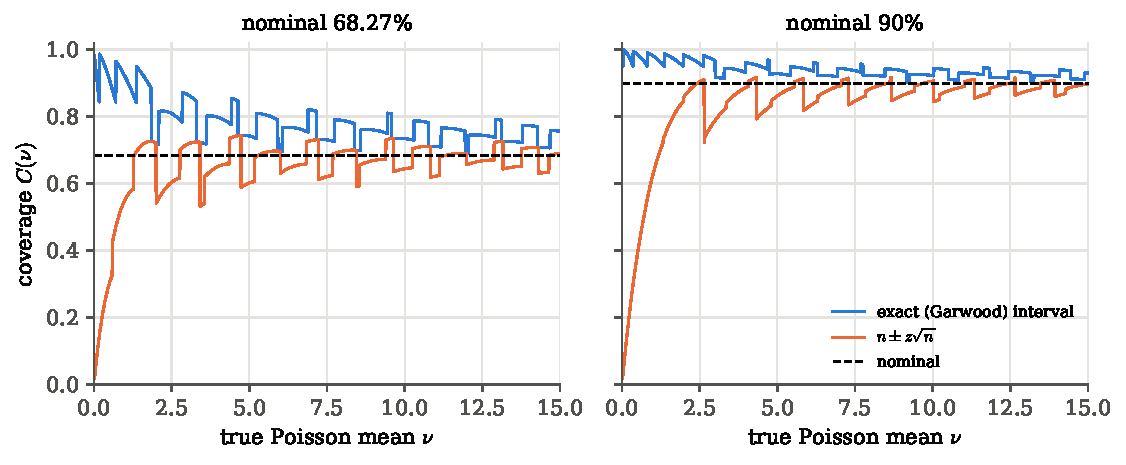
\includegraphics[width=\linewidth]{figures/ch04/coverage_poisson.pdf}
\caption{Exact coverage of two interval recipes for a Poisson mean, as a
function of the true mean. Left: nominal $68.27\%$, right: nominal $90\%$
(dashed lines). Garwood's exact interval (blue) always lies above the nominal
level, with saw-tooth jumps where the true mean crosses an interval end. The
quick interval $n\pm z\sqrt n$ (orange) undercovers, dramatically so below a
mean of about two.}
\label{4b:fig:coverage-poisson}
\end{figure}

The script \pyname{code/ch04/13_coverage.py} computes these curves with a
matrix of Poisson probabilities:

\pyfile[firstline=66,lastline=87,label={4b:lst:coverage}]{code/ch04/13_coverage.py}{Exact coverage of Poisson interval recipes}

Each recipe returns the interval ends for all counts $0,\dots,80$ at once. The
boolean matrix \pyname{inside} has one row per true $\nu$ and one column per
count, and is true where that count's interval contains that $\nu$.
Multiplying by the Poisson probabilities and summing along each row is
\eqref{4b:eq:coverage-function}. A brute-force check at $\nu=\FourBNuChk$ draws
$\FourBSims$ counts, builds their intervals and counts hits: the Monte Carlo
coverage $\FourBCovChkMC$ agrees with the exact $\FourBCovChkExact$ (and for the
quick recipe the simulation gives $\FourBCovChkMCw$).

\paragraph{Pointwise versus uniform.}
The Poisson curve makes concrete a distinction between two meanings of
``correct for large samples'' \mainref{\S6.5}. Take the Normal interval for a
proportion $p$ from $n$ trials, with estimate $\hat p$ and coverage $C(p)$.
For each \emph{fixed} $p$, $C(p)$ tends to $1-\alpha$ as $n\to\infty$: the
interval is \emph{pointwise} asymptotic. But at any fixed $n$, a small enough
$p$ makes $\hat p=0$ almost certain; the interval then collapses to $\{0\}$,
and the coverage is near zero. So the worst case $\inf_pC(p)$ does not tend to
$1-\alpha$, and the interval is not \emph{uniformly} asymptotic. ``Large sample'' has to be
large compared with something, and near a boundary the something is the
number of events, not the number of trials.

\subsection{Right on average, wrong in a recognisable case}
\label{4b:sec:berger-wolpert}

Coverage is an average over all possible data sets. Sometimes the data we hold
tell us that we are in a subset of those data sets where the recipe is right
much more often, or much less often, than the average. An example due to
Berger and Wolpert shows this plainly \mainref{Ex.~6.14}. Let $\theta$ be a
fixed number, let
$X_1,X_2$ be independent, each $+1$ or $-1$ with probability one half, and
observe only $Y_i=\theta+X_i$. The ``interval'', a single point, is
\[
  C=\begin{cases}\{Y_1-1\} & \text{if }Y_1=Y_2,\\ \{(Y_1+Y_2)/2\} & \text{if }Y_1\ne Y_2.\end{cases}
\]
There are four equally likely cases:
\begin{align}
  \Prob_\theta(\theta\in C)
  &\eqby{1} \tfrac14\,\mathbb 1[(\theta+1)-1=\theta]
          +\tfrac14\,\mathbb 1[(\theta-1)-1=\theta]
          +\tfrac24\,\mathbb 1[\tfrac12(2\theta)=\theta]
   \eqby{2} \tfrac14+0+\tfrac12=\tfrac34 .
  \label{4b:eq:bw}
\end{align}
\begin{explain}
  \item $(X_1,X_2)=(+1,+1)$: both $Y$ equal $\theta+1$, and $C=\{\theta\}$.
        $(-1,-1)$: both equal $\theta-1$, and $C=\{\theta-2\}$. $(+1,-1)$ or
        $(-1,+1)$: the $Y$ differ and their average is $\theta$.
  \item Evaluate the indicators.
\end{explain}
So $C$ is a $75\%$ confidence set for every $\theta$.

\emph{What we observe.} Now suppose the data are $Y_1=15$, $Y_2=17$.
\emph{The question.} Which of the four cases could have produced these data?
The two $Y$ differ, so $(+1,+1)$ and $(-1,-1)$ are ruled out; only the mixed
cases remain, and in both of them the average of the $Y$ is $\theta$. So
$C=\{16\}$ is \emph{certainly} right. Had we instead seen $Y_1=Y_2$, only the
first two cases could have produced it, and the recipe is right in one of them
and wrong in the other: right half the time. A simulation of $4\times10^5$ repetitions in
\pyname{code/ch04/11_test_inversion.py} confirms it: overall coverage
$\FourBBWcovAll$, coverage $\FourBBWcovDiff$ when $Y_1\ne Y_2$ (a fraction
$1-\FourBBWfracSame$ of the time), and $\FourBBWcovSame$ when $Y_1=Y_2$.

The lesson: ``$75\%$'' is a statement about the recipe, not about this data
set. Calling $\{16\}$ a $75\%$ confidence set is still correct, because that is
what the recipe guarantees \mainref{p.~93}. A probability statement about
$\theta$ given these particular $Y$ is a different kind of statement, the one
Bayesian inference makes (\cref{4b:sec:credible}). Frequentists handle the
problem by \emph{conditioning}: they compute the coverage only over data sets
that share a feature of the observed one, a feature that carries no information
about $\theta$ but does tell us how precise the experiment turned out to be
(here, whether $Y_1=Y_2$). In physics the classic case is a measurement whose
resolution depends on an event-by-event quantity: the relevant error bar is the
one for the resolution actually obtained.

\begin{inpractice}[Coverage studies: verification and research]
A coverage simulation can play two different roles. When an analytic result
exists, it \emph{verifies}: the $t$ interval must cover $95\%$ at every $n$, the
Garwood interval must never undercover, and a simulation that disagrees has a
bug. When no analytic result exists, the same simulation \emph{is} the method.
Experiments at the LHC build Neyman belts from toy Monte Carlo when the test
statistic has no known distribution; neutrino-oscillation fits construct
Feldman--Cousins regions from millions of pseudo-experiments; cosmological
analyses check whether a posterior interval from an MCMC chain
(\cref{ch:09}) covers the input parameters of simulated skies. In every case the
recipe is \eqref{4b:eq:coverage-function} evaluated by brute force.
\end{inpractice}
\section{Upper limits near a physical boundary}
\label{4b:sec:boundary}

The squared mass of a neutrino can be estimated from a measured energy and
momentum as $\widehat{m^2}=E^2-p^2$. The true $m^2$ cannot be negative, but the
estimate can: both $E^2$ and $p^2$ carry measurement errors, and when the true
mass is tiny, their difference comes out negative about half the time
\srcref{Cowan}{\S9.8}. The same happens to any parameter estimated as a
difference, $\hat\theta=x-y$: a signal rate estimated as ``counts minus
expected background'', a dark-matter cross-section, a tensor-to-scalar ratio.
Physics says $\theta\ge0$. The data, fluctuating, do not know that.

A search that sees nothing reports an \emph{upper limit}. Near the boundary
every recipe met so far runs into trouble. The interval can come out entirely
in the forbidden region, or be empty, or be so short that it claims more than
the experiment can know. Each fix trades one good property for another, and
seeing what each one gives up shows what a limit really promises.

\paragraph{The question in words.}
\begin{enumerate}[label=\arabic*.]
  \item What does the classical recipe give when the estimate is negative, and
        is it wrong?
  \item Which alternatives exist (shifting the estimate, a Bayesian prior on
        $\theta\ge0$, Feldman and Cousins' ordering, CL$_s$), and what does
        each do to the coverage?
  \item Why must the choice between ``upper limit'' and ``two-sided interval''
        be made before the data are seen?
\end{enumerate}

\subsection{The classical limit can be negative}
\label{4b:sec:classical-limit}

Let $\hat\theta$ be Gaussian with mean $\theta$ and known $\sigma_{\hat\theta}$,
with $\theta\ge0$ known a priori. The one-sided classical upper limit at
confidence level $1-\beta$ is, from \eqref{4b:eq:gauss-ends},
\begin{equation}
  \theta_{\rm up}=\hat\theta_{\rm obs}+\sigma_{\hat\theta}\,\Phi^{-1}(1-\beta)
  \label{4b:eq:classical-up}
\end{equation}
\srcref{Cowan}{(9.39)}. With $\sigma_{\hat\theta}=1$ and
$\hat\theta_{\rm obs}=-2$, the $95\%$ limit is
$-2+1.645=\FourBBdUpNinetyFive$. The experiment ``excludes'' every physical
value of $\theta$, including zero.

\emph{Is the recipe wrong?} No. It covers the true value in $95\%$ of
experiments, whatever that value is. If $\theta=0$, an estimate below $-1.645$
happens $5\%$ of the time, and those are exactly the experiments whose limit
is negative. We have simply landed in the $5\%$. \emph{Is the result useful?}
Also no. We knew before the experiment that $\theta\ge0$, and so certainly
that $\theta>\FourBBdUpNinetyFive$. Two tempting repairs make it worse. Raising the
confidence level to $99\%$ moves the limit to $\FourBBdUpNinetyNine$, a limit
three times smaller than the experiment's resolution, quoted at very high
confidence; and choosing the level $97.725\%$ gives $\theta_{\rm up}=10^{-5}$,
which is absurd \srcref{Cowan}{p.~137}.

Whatever limit we quote, the first rule is to report the estimate itself,
$\hat\theta_{\rm obs}\pm\sigma_{\hat\theta}$, even when it is negative. The
reason is combination. Unbiased estimates from many experiments average to the
truth only if the negative ones are kept; setting them to zero pushes every
average upwards. When
$\hat\theta$ is far from Gaussian, the whole likelihood function should be
published so that others can combine it \srcref{Cowan}{p.~137}.

\subsection{Three repairs: shift, Bayes, and flip-flop}
\label{4b:sec:repairs}

\paragraph{Shift the estimate to zero.}
A common practice replaces a negative estimate by zero before applying
\eqref{4b:eq:classical-up} \srcref{Cowan}{(9.40)}:
$\theta_{\rm up}=\max(\hat\theta_{\rm obs},0)+\sigma_{\hat\theta}\Phi^{-1}(1-\beta)$.
At $95\%$ the limit is then never below $1.645\,\sigma_{\hat\theta}$
($\FourBBdUpShift$ for our example), so it is never smaller than about the
resolution. The shifted limit is never below the classical one, so it contains
the truth at least as often: it overcovers. In \cref{4b:fig:boundary} (right) its coverage is $1$ for all
$\theta\le1.645$, because every experiment then quotes a limit above $\theta$.

\paragraph{A Bayesian limit with a prior that knows $\theta\ge0$.}
In the Bayesian approach the boundary is built in by a prior that vanishes for
$\theta<0$. With a flat prior on $\theta\ge0$ \srcref{Cowan}{(9.41)--(9.44)} and
$\sigma_{\hat\theta}=1$, the posterior is the Gaussian likelihood cut off at
zero and renormalised. Write $x=\hat\theta_{\rm obs}$ and $\varphi$ for the
standard normal density. The upper limit solves
\begin{align}
  1-\beta
  &\eqby{1} \frac{\int_0^{\theta_{\rm up}}\varphi(\theta-x)\,\dd\theta}{\int_0^{\infty}\varphi(\theta-x)\,\dd\theta}
   \eqby{2} \frac{\Phi(\theta_{\rm up}-x)-\Phi(-x)}{1-\Phi(-x)}
   \eqby{3} \frac{\Phi(\theta_{\rm up}-x)-1+\Phi(x)}{\Phi(x)} ,
  \notag\\
  \Longrightarrow\quad
  \theta_{\rm up}
  &\eqby{4} x+\Phi^{-1}\bigl(1-\beta\,\Phi(x)\bigr).
  \label{4b:eq:bayes-up}
\end{align}
\begin{explain}
  \item Bayes' theorem with a flat prior on $\theta\ge0$: the posterior is the
        likelihood $\varphi(\theta-x)$ normalised over the physical region
        \srcref{Cowan}{(9.43)}.
  \item Substitute $t=\theta-x$; the integrals are differences of the normal
        CDF.
  \item Symmetry, $\Phi(-x)=1-\Phi(x)$, in numerator and denominator.
  \item Multiply by $\Phi(x)$, solve for $\Phi(\theta_{\rm up}-x)=1-\beta\Phi(x)$,
        and apply $\Phi^{-1}$.
\end{explain}
For $x=-2$ this gives $\theta_{\rm up}=\FourBBdUpBayes$. For large positive $x$,
$\Phi(x)\to1$ and the limit tends to the classical $x+1.645$. The Bayesian limit
is always positive and always above the classical one (Cowan's Fig.~9.8, our
\cref{4b:fig:boundary}, left).

It means something different. It is the value that $\theta$ exceeds with
posterior probability $5\%$, given the prior. So it depends on the prior, and
the flat prior has two weaknesses. First, it says that $0<\theta<1$ is as
plausible before the experiment as $10^{40}<\theta<10^{40}+1$. Second, it
changes when we relabel the parameter: a flat prior on $m^2$ is not flat on
$m$. The prior
$\pi(\theta)\propto1/\theta$, flat in $\ln\theta$, gives limits invariant under
$\theta\to\theta^k$, but the integrals diverge unless the likelihood vanishes
at $\theta\to0$, which a Gaussian likelihood does not
\srcref{Cowan}{(9.45) and p.~139}. In practice the flat prior is the common
choice, with its assumptions stated.

The Bayesian limit was not built to have coverage, but we can still measure
its coverage. \Cref{4b:fig:boundary} (right) shows that for this problem it
overcovers near the boundary and approaches $95\%$ from above for large
$\theta$ (minimum $\FourBBdCovBayesMin$).

\begin{figure}[htbp]
\centering
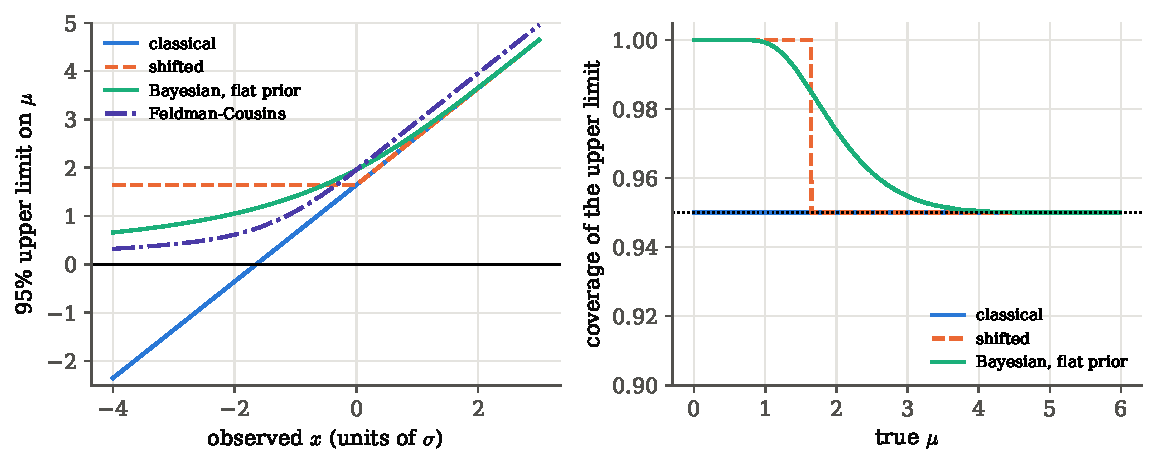
\includegraphics[width=\linewidth]{figures/ch04/boundary_limits.pdf}
\caption{Left: $95\%$ upper limits on a non-negative Gaussian mean as a
function of the observed estimate, in units of the resolution. The classical
limit (blue) goes negative for estimates below $-1.645$; the shifted limit
(orange dashed) is flat at $1.645$ for negative estimates; the flat-prior
Bayesian limit (green) and the Feldman--Cousins upper end (violet) stay positive
and fall slowly. All agree for large estimates. Right: the coverage of three of
the recipes as a function of the true value. The classical limit covers exactly
$95\%$, the other two more near the boundary.}
\label{4b:fig:boundary}
\end{figure}

\paragraph{Flip-flopping.}
Feldman and Cousins describe a third habit, common enough that they gave it a
name \cite{FeldmanCousins1998}. Physicist X decides after seeing the data: ``if
the result is less than $3\sigma$, I quote a $90\%$ upper limit; if it is more,
I quote a $90\%$ central interval; and if it is negative, I pretend it was
zero.'' Each of the two recipes alone covers $90\%$. The mixture does not.
\emph{The question:} take $\sigma=1$ and a true mean $\mu=2$; how often does the
mixture contain $2$? Here $x$ is the measured value. Take the two branches one
at a time.
\begin{itemize}[itemsep=1pt,leftmargin=1.2em]
  \item The upper-limit branch ($x<3$) quotes $[0,\max(x,0)+1.28]$, which
        contains $2$ when $x\ge0.72$.
  \item The central branch ($x\ge3$) quotes $[x-1.645,x+1.645]$, which
        contains $2$ when $x\le3.645$.
\end{itemize}
So
\begin{align}
  C(2)
  &\eqby{1} \Prob(0.72\le x<3)+\Prob(3\le x\le3.645)
   \eqby{2} \Prob(-1.28\le x-2\le1.645)
   \notag\\
  &\eqby{3} \Phi(1.645)-\Phi(-1.28)
   \eqby{4} 0.95-0.10=0.85 .
  \label{4b:eq:flipflop}
\end{align}
\begin{explain}
  \item The two branches, each with its own condition for covering $\mu=2$.
  \item The two ranges join into one; subtract the true value $2$.
  \item $x-2$ is standard normal.
  \item The standard quantiles of \cref{4b:sec:belt-gauss}.
\end{explain}
The quoted ``$90\%$'' intervals cover $85\%$ of the time. The missing $5\%$ are
the measurements above $3.645$. The upper-limit recipe alone would have given
them a limit above $2$, but the switch hands them a central interval that
misses. The script finds the
same $\FourBFfCovTwo$ at $\mu=2$, and that this is the minimum; the coverage stays
at $85\%$ from $\mu\approx1.3$ to $\mu\approx4.3$ (\cref{4b:fig:fc-coverage},
left). In belt language (\cref{4b:fig:fc-belts}, dashed), switching recipes
at $x=3$ bends the belt so that the horizontal acceptance intervals at
intermediate $\mu$ hold only $85\%$ of the probability.

\begin{pitfall}[Deciding the form of the result after seeing the data]
Choosing between an upper limit and a two-sided interval according to how the
data came out destroys the coverage of both, even though each recipe is
correct alone. The rule of the Neyman construction is that the acceptance
regions are fixed before the measurement. If we want the result to switch
automatically from a limit to an interval as the signal grows, the switch must
be part of the construction itself, which is what the unified approach below
does.
\end{pitfall}

The strict alternative, always quoting the central interval, has its own
problem. With $\sigma=1$ and $x=-1.8$, the $90\%$ central interval has upper end
$x+1.645=-0.155$, so it contains no physical value at all. The interval is
\emph{empty} \cite{FeldmanCousins1998}. It is still a correct member of an
ensemble with $90\%$ coverage, but not one anybody wants to publish.

\subsection{The unified approach of Feldman and Cousins}
\label{4b:sec:fc}

The Neyman construction (\cref{4b:sec:belt}) leaves one choice open:
\emph{which} values of the measurement to put in the acceptance interval at
each $\mu$, so that it holds probability $1-\alpha$. Central intervals leave
out equal tails on both sides; upper limits leave out only the lowest values,
keeping everything above a cut. Feldman and Cousins choose by a likelihood ratio.

\begin{keyidea}[Likelihood-ratio ordering]
At each $\mu$, rank the possible outcomes $x$ by
\[
  R(x)=\frac{P(x\given\mu)}{P(x\given\mu_{\rm best})},
\]
where $\mu_{\rm best}$ is the \emph{physically allowed} value of $\mu$ that
makes $x$ most probable. Add outcomes to the acceptance interval in order of
decreasing $R$ until their total probability reaches $1-\alpha$
\cite[(4.1)]{FeldmanCousins1998}. Then build the belt and read the intervals as
usual. The coverage is right by construction, the interval is never empty, and
the result turns by itself from an upper limit into a two-sided interval as the
data move away from the boundary.
\end{keyidea}

\emph{Why this ordering?} $R$ compares how well $\mu$ explains $x$ with how
well the best physical value explains it. An outcome with $R$ close to one is
one that $\mu$ explains nearly as well as any allowed value could. Putting such
outcomes in the acceptance set first means that we reject $\mu$ only for data
that some other physical $\mu$ explains much better. This is the likelihood-ratio test of the
first part of the chapter, with the physical boundary written into the
maximisation, inverted into an interval.

\paragraph{Gaussian with $\mu\ge0$.}
With $P(x\given\mu)=\varphi(x-\mu)$, the best physical value is
$\mu_{\rm best}=\max(0,x)$. Then
\begin{align}
  R(x)
  &\eqby{1}
   \begin{cases}
     \varphi(x-\mu)/\varphi(0)=e^{-(x-\mu)^2/2}, & x\ge0,\\[2pt]
     \varphi(x-\mu)/\varphi(x)=e^{-(x-\mu)^2/2+x^2/2}=e^{\,x\mu-\mu^2/2}, & x<0,
   \end{cases}
  \label{4b:eq:fc-R}
\end{align}
\begin{explain}
  \item For $x\ge0$, $\mu_{\rm best}=x$ and $\varphi(0)=1/\sqrt{2\pi}$; for $x<0$,
        $\mu_{\rm best}=0$, and expanding $-(x-\mu)^2/2+x^2/2=x\mu-\mu^2/2$
        \cite[(4.2)--(4.3)]{FeldmanCousins1998}.
\end{explain}
For $x\ge0$, $R$ decreases with the distance from $\mu$, so the acceptance
interval is centred, as in a central interval. For $x<0$, $R$ decreases as $x$
becomes more negative, but only linearly in the exponent, much more slowly than
the Gaussian: negative outcomes are penalised less, because no physical $\mu$
explains them well. The acceptance interval $[x_1,x_2]$ at each $\mu$ is found
numerically from $R(x_1)=R(x_2)$ and $\int_{x_1}^{x_2}\varphi(x-\mu)\dd x=1-\alpha$
\cite[(4.4)]{FeldmanCousins1998}.

\emph{Where does the limit turn into a two-sided interval?} The acceptance
set at $\mu=0$ decides it. There $R(x)=1$ for all
$x<0$ and $R(x)=e^{-x^2/2}$ for $x\ge0$, so every negative $x$ is ranked first
(probability $1/2$), followed by $x$ from $0$ upwards until the total is $0.90$:
$\Phi(x_2)=0.90$, $x_2=\FourBFcTrans$. For an observation above $\FourBFcTrans$,
$\mu=0$ is excluded and the interval is two-sided; below it, the interval starts
at zero and is an upper limit. The brute-force belt in
\pyname{code/ch04/15_feldman_cousins.py} reproduces Feldman and Cousins' Table~X
at $90\%$:
\begin{center}
\begin{tabular}{lcccccc}
\toprule
$x_0$ & $-2$ & $-1$ & $0$ & $1$ & $2$ & $3$\\
\midrule
$[\mu_1,\mu_2]$ &
$[\FourBFcGMinusTwoLo,\FourBFcGMinusTwoHi]$ &
$[\FourBFcGMinusOneLo,\FourBFcGMinusOneHi]$ &
$[\FourBFcGZeroLo,\FourBFcGZeroHi]$ &
$[\FourBFcGOneLo,\FourBFcGOneHi]$ &
$[\FourBFcGTwoLo,\FourBFcGTwoHi]$ &
$[\FourBFcGThreeLo,\FourBFcGThreeHi]$\\
\bottomrule
\end{tabular}
\end{center}
Here $x_0$ is the observed measurement and $[\mu_1,\mu_2]$ its interval. At
$x_0=0$ the $90\%$ upper limit is $\FourBFcGZeroHi$: the classical $95\%$ limit
rather than the $90\%$ one ($1.28$). The reason is that at $\mu\approx1.6$ the
unified acceptance interval is already nearly central, so its left edge sits
$1.645$ below $\mu$, and $1.645$ is also the one-sided $95\%$ quantile
(\cref{4b:sec:belt-gauss}). That is the price of repairing flip-flopping: near
the boundary the unified limits are somewhat looser
\cite{FeldmanCousins1998}. In exchange no interval is empty, the limits for
very negative $x_0$ shrink only slowly (as $1/\abs{x_0}$), and the coverage is
$90\%$ for every $\mu$ (between $\FourBFcCovMin$ and $\FourBFcCovMax$ on our grid;
\cref{4b:fig:fc-coverage}, left).

\begin{figure}[htbp]
\centering
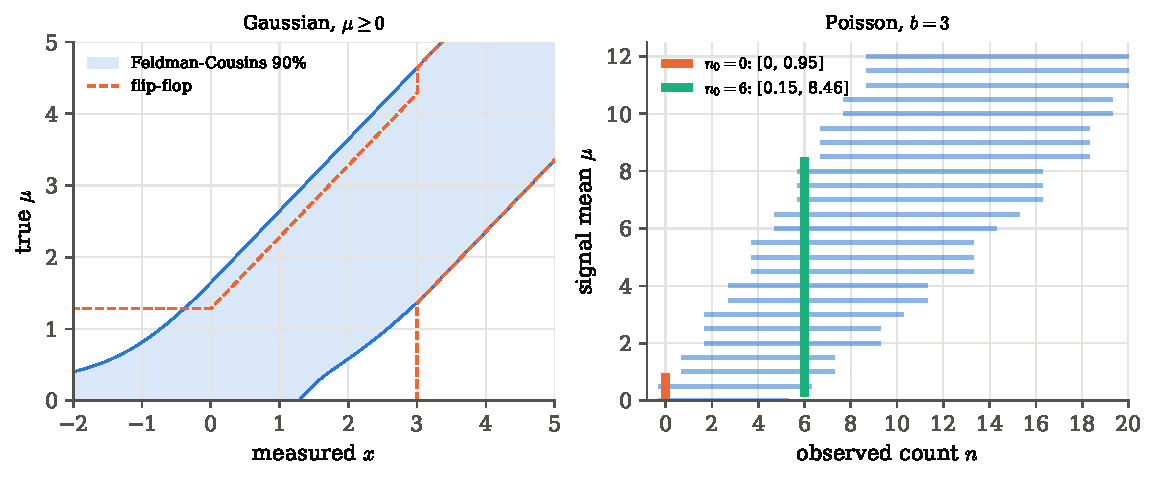
\includegraphics[width=\linewidth]{figures/ch04/fc_belts.pdf}
\caption{Left: the $90\%$ Feldman--Cousins belt for a Gaussian measurement of a
non-negative mean (shaded, solid edges) and the belt implied by flip-flopping
(dashed). Below $x\approx1.28$ the unified belt reaches down to $\mu=0$, so the
interval is an upper limit; above, it is two-sided. The flip-flop belt jumps at
$x=3$ where the recipe switches. Right: the Feldman--Cousins acceptance sets
for a Poisson count on a known background $b=3$ (bars every $0.5$ in $\mu$),
with the intervals for $n_0=0$ (orange) and $n_0=6$ (green).}
\label{4b:fig:fc-belts}
\end{figure}

\subsection{Counting on a known background}
\label{4b:sec:fc-poisson}

The most common version of the problem in particle physics is a count $n$ of
candidate events, of which a known mean $b$ is expected from background and an
unknown mean $\mu\ge0$ from signal \srcref{Cowan}{\S9.9}. The total is Poisson
with mean $\mu+b$,
\begin{equation}
  P(n\given\mu)=\frac{(\mu+b)^n}{n!}\,e^{-(\mu+b)} ,
  \label{4b:eq:poisson-bkg}
\end{equation}
and the naive estimate is $\hat\mu=n-b$, which is negative whenever fewer
events than the expected background are seen \srcref{Cowan}{(9.47)--(9.48)}.
The classical limits are the background-free ones shifted down by $b$
\srcref{Cowan}{(9.50)}. For $b=3$ and no events observed, the $90\%$ upper
limit is $\FourBUpNinetyZero-3=\FourBPtClZero$: negative. The central $90\%$
interval is $[0,\ 3.00-3]$, with an upper end $\FourBPtCentralUpZero$ below zero:
empty \cite{FeldmanCousins1998}.

\paragraph{The ordering at one value of $\mu$.}
Feldman and Cousins work one row of their construction by hand, $b=3$ and
$\mu=0.5$ \cite[Table~I]{FeldmanCousins1998}. For each $n$ the best physical
signal is $\mu_{\rm best}=\max(0,n-b)$, and $R=P(n\given0.5)/P(n\given\mu_{\rm best})$:
\begin{center}
\small
\begin{tabular}{l*{11}{c}}
\toprule
$n$ & 0 & 1 & 2 & 3 & 4 & 5 & 6 & 7 & 8 & 9 & 10\\
\midrule
$P(n\given\mu)$ & $\FourBPtPZero$ & $\FourBPtPOne$ & $\FourBPtPTwo$ & $\FourBPtPThree$ & $\FourBPtPFour$ & $\FourBPtPFive$ & $\FourBPtPSix$ & $\FourBPtPSeven$ & $\FourBPtPEight$ & $\FourBPtPNine$ & $\FourBPtPTen$\\
$\mu_{\rm best}$ & 0 & 0 & 0 & 0 & 1 & 2 & 3 & 4 & 5 & 6 & 7\\
$R$ & $\FourBPtRZero$ & $\FourBPtROne$ & $\FourBPtRTwo$ & $\FourBPtRThree$ & $\FourBPtRFour$ & $\FourBPtRFive$ & $\FourBPtRSix$ & $\FourBPtRSeven$ & $\FourBPtREight$ & $\FourBPtRNine$ & $\FourBPtRTen$\\
rank & $\FourBPtRankZero$ & $\FourBPtRankOne$ & $\FourBPtRankTwo$ & $\FourBPtRankThree$ & $\FourBPtRankFour$ & $\FourBPtRankFive$ & $\FourBPtRankSix$ & $\FourBPtRankSeven$ & $\FourBPtRankEight$ & $\FourBPtRankNine$ & $\FourBPtRankTen$\\
\bottomrule
\end{tabular}
\end{center}
Adding counts in the order of the last row, the total first reaches $0.90$ with
rank $7$, so the acceptance set at $\mu=0.5$ is $n\in[\FourBPtAccLo,\FourBPtAccHi]$,
with probability $\FourBPtAcc$ (more than $0.90$, because of discreteness).
Look at $n=0$. Its probability under $\mu=0.5$ is only $0.030$. But no physical
$\mu$ makes it much more probable: the best is $\mu=0$, with $0.050$. So
$R=\FourBPtRZero$, high in the ranking, and $n=0$ is accepted. This is what
keeps the interval for $n_0=0$ from being empty.

\paragraph{The intervals.}
Repeating the ranking on a grid of $\mu$ and reading vertically gives the
Feldman--Cousins intervals; \cref{4b:fig:fc-belts} (right) shows the belt. The
code is short:

\pyfile[firstline=143,lastline=154,label={4b:lst:fc}]{code/ch04/15_feldman_cousins.py}{The Feldman--Cousins acceptance sets for a Poisson count on background}

For every $n$ the array \pyname{pbest} holds $P(n\given\mu_{\rm best})$; for each
hypothetical $\mu$ the counts are sorted by decreasing $R$ (\pyname{argsort} of
$-R$), their probabilities accumulated, and the set cut where the running sum
first reaches the confidence level. The minimum and maximum of the kept counts
are the ends of the horizontal set. For $b=3$ at $90\%$:
\begin{center}
\small
\begin{tabular}{l*{11}{c}}
\toprule
$n_0$ & 0 & 1 & 2 & 3 & 4 & 5 & 6 & 7 & 8 & 9 & 10\\
\midrule
FC $\mu_1$ & $\FourBPtFCZeroLo$ & $\FourBPtFCOneLo$ & $\FourBPtFCTwoLo$ & $\FourBPtFCThreeLo$ & $\FourBPtFCFourLo$ & $\FourBPtFCFiveLo$ & $\FourBPtFCSixLo$ & $\FourBPtFCSevenLo$ & $\FourBPtFCEightLo$ & $\FourBPtFCNineLo$ & $\FourBPtFCTenLo$\\
FC $\mu_2$ & $\FourBPtFCZeroHi^{*}$ & $\FourBPtFCOneHi$ & $\FourBPtFCTwoHi$ & $\FourBPtFCThreeHi$ & $\FourBPtFCFourHi$ & $\FourBPtFCFiveHi$ & $\FourBPtFCSixHi$ & $\FourBPtFCSevenHi$ & $\FourBPtFCEightHi$ & $\FourBPtFCNineHi$ & $\FourBPtFCTenHi$\\
classical & $\FourBPtClZero$ & $\FourBPtClOne$ & $\FourBPtClTwo$ & $\FourBPtClThree$ & $\FourBPtClFour$ & $\FourBPtClFive$ & $\FourBPtClSix$ & $\FourBPtClSeven$ & $\FourBPtClEight$ & $\FourBPtClNine$ & $\FourBPtClTen$\\
CL$_s$ & $\FourBPtCLsZero$ & $\FourBPtCLsOne$ & $\FourBPtCLsTwo$ & $\FourBPtCLsThree$ & $\FourBPtCLsFour$ & $\FourBPtCLsFive$ & $\FourBPtCLsSix$ & $\FourBPtCLsSeven$ & $\FourBPtCLsEight$ & $\FourBPtCLsNine$ & $\FourBPtCLsTen$\\
\bottomrule
\end{tabular}
\end{center}
The first two rows agree with Feldman and Cousins' Table~IV to the grid
precision, with one exception marked $^{*}$. For $n_0=0$ the raw construction
gives $\FourBPtFCZeroHiRaw$; Feldman and Cousins publish $1.08$. The difference is
a deliberate correction: because $n$ is discrete, the raw upper end is not always
a decreasing function of $b$, and they lengthen intervals to make it so. Applying
their rule (replace $\mu_2(b)$ by the largest value at any larger background) on
a fine grid of $b$ gives $\FourBPtFCZeroHiFixed$. For $n_0\le5$ the interval starts
at zero: an upper limit. From $n_0=6$ on it is two-sided. The switch happens by
itself.

\paragraph{CL$_s$ and the Bayesian limit.}
The classical limit in the third row goes negative for small $n_0$. The reason:
when the background fluctuates down, few events are seen, and every signal
looks excluded. The LEP and Tevatron experiments adopted a modification
designed against exactly this \cite{Cowan2011}. In a counting experiment, a
small $n$ is what argues against a signal, so the two relevant tail
probabilities are those of seeing $n_0$ or fewer events, with and without the
signal:
\begin{equation}
  \mathrm{CL}_{s+b}(\mu)=\Prob(n\le n_0\given\mu+b),
  \qquad
  \mathrm{CL}_b=\Prob(n\le n_0\given b).
  \label{4b:eq:clsb}
\end{equation}
The classical recipe excludes $\mu$ when $\mathrm{CL}_{s+b}<\alpha$.

\begin{workdef}[CL$_s$]
The ratio $\mathrm{CL}_s(\mu)=\mathrm{CL}_{s+b}(\mu)/\mathrm{CL}_b$ (in the
notation of \cite{Cowan2011}, $p_{s+b}/(1-p_b)$). A signal $\mu$ is excluded at
confidence level $1-\alpha$ if $\mathrm{CL}_s(\mu)<\alpha$. Dividing by
$\mathrm{CL}_b\le1$ makes exclusion harder exactly when the data look
background-poor \unpack{when even background alone rarely gives so few events}.
\end{workdef}

For $n_0=0$, $\mathrm{CL}_s=e^{-(\mu+b)}/e^{-b}=e^{-\mu}$, and the $90\%$ limit is
$\mu=\ln10=\FourBPtCLsZero$ for \emph{every} $b$. Seeing nothing on a background of
three events excludes no more than seeing nothing on no background. That is the
intended behaviour: an experiment should not get a better limit because its
background fluctuated low. \Cref{4b:fig:fc-limits} contrasts the three
recipes as a function of $b$. The classical limit for $n_0=0$ falls as
$2.30-b$ and crosses zero at $b=2.30$. The Feldman--Cousins limit also falls, from
$\FourBPtFCUpZeroBzero$ at $b=0$ towards about one: it is a correct confidence
interval, and with a larger background, zero events really are rarer for every
$\mu$. CL$_s$ stays at $\FourBPtCLsZero$.

The CL$_s$ limit is the flat-prior Bayesian limit of Cowan's (9.53)--(9.54).
With a flat prior on $\mu\ge0$, the posterior probability above $\mu$ is
\begin{align}
  \Prob(\mu_s>\mu\given n_0)
  &\eqby{1} \frac{\int_\mu^\infty(\mu'+b)^{n_0}e^{-(\mu'+b)}\,\dd\mu'}{\int_0^\infty(\mu'+b)^{n_0}e^{-(\mu'+b)}\,\dd\mu'}
   \eqby{2} \frac{\int_{\mu+b}^\infty t^{n_0}e^{-t}\,\dd t/n_0!}{\int_{b}^\infty t^{n_0}e^{-t}\,\dd t/n_0!}
  \notag\\
  &\eqby{3} \frac{\sum_{n=0}^{n_0}(\mu+b)^ne^{-(\mu+b)}/n!}{\sum_{n=0}^{n_0}b^ne^{-b}/n!}
   \eqby{4} \mathrm{CL}_s(\mu).
  \label{4b:eq:cls-bayes}
\end{align}
\begin{explain}
  \item Posterior tail with the likelihood \eqref{4b:eq:poisson-bkg}; the
        $1/n_0!$ cancels.
  \item Substitute $t=\mu'+b$, and divide top and bottom by $n_0!$.
  \item The gamma tail equals the Poisson cumulative sum,
        $\int_x^\infty t^ke^{-t}\dd t/k!=\sum_{n=0}^k x^ne^{-x}/n!$: this is
        \eqref{4b:eq:poisson-chi2} with $z=2t$, since
        $f_{\chi^2}(2t;2k+2)\,\dd(2t)=t^ke^{-t}\dd t/k!$.
  \item Definition \eqref{4b:eq:clsb}.
\end{explain}
So setting the posterior tail to $\alpha$ and setting CL$_s=\alpha$ give the same
limit; the script finds the two limits equal to within $\FourBPtCLsBayesDiff$. For $b=0$
both reduce to the classical limit \srcref{Cowan}{(9.55)}, because then
$\mathrm{CL}_b=1$. So for a counting experiment without background the
frequentist and the flat-prior Bayesian limits are the same number, and there
is no choice to make \srcref{Cowan}{p.~142}.

\begin{figure}[htbp]
\centering
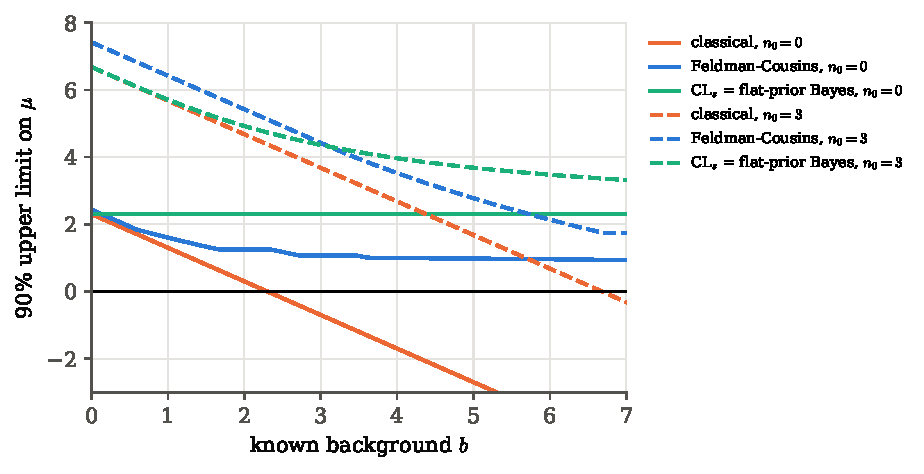
\includegraphics[width=0.78\linewidth]{figures/ch04/fc_poisson_limits.pdf}
\caption{$90\%$ upper limits on a signal mean for $n_0=0$ (solid) and $n_0=3$
(dashed) observed events, as a function of the known background. The classical
limit (orange) falls linearly and becomes negative; the Feldman--Cousins limit
(blue) falls but stays positive; CL$_s$, equal to the flat-prior Bayesian
limit (green), does not improve when the background grows: for $n_0=0$ it is
flat at $2.30$.}
\label{4b:fig:fc-limits}
\end{figure}

\paragraph{What each recipe does to the coverage.}
\Cref{4b:fig:fc-coverage} (right) shows the exact coverage for $b=3$. All three
recipes keep $90\%$ as a minimum (Feldman--Cousins $\FourBPtCovFCMin$, classical
$\FourBPtCovClMin$, CL$_s$ $\FourBPtCovCLsMin$) and all have the Poisson
saw-tooth. They differ in how much they overcover. The classical limit,
negative values and all, is a correct $90\%$ upper limit; its failures include
every experiment that quotes a negative limit. CL$_s$ overcovers most near
$\mu=0$, where it always covers, because it never excludes any $\mu$ below
$2.30$. It is conservative by design: not a confidence interval in the strict
Neyman sense, but a limit with guaranteed coverage that a lucky downward
fluctuation cannot improve. Feldman--Cousins is closest to exact.

\begin{figure}[htbp]
\centering
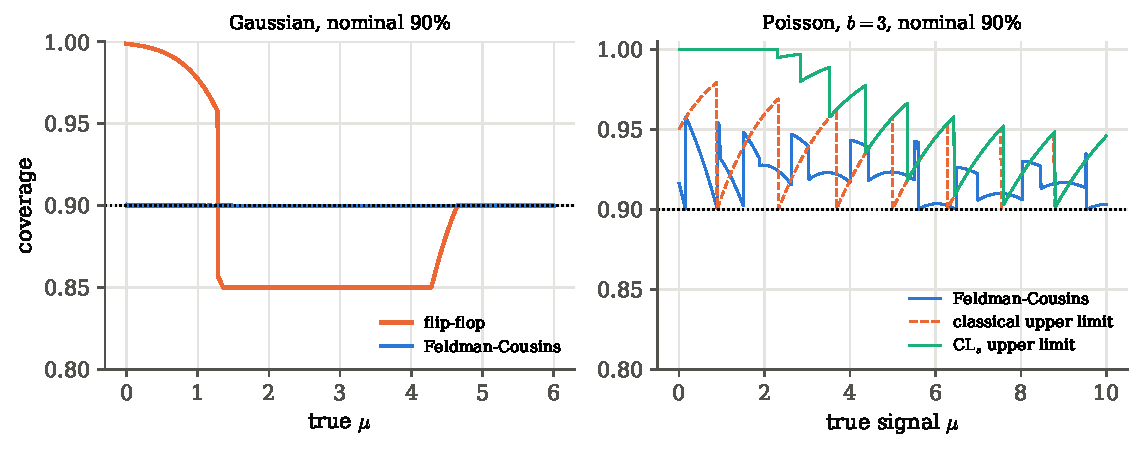
\includegraphics[width=\linewidth]{figures/ch04/fc_coverage.pdf}
\caption{Coverage near a boundary. Left: Gaussian measurement of a non-negative
mean, nominal $90\%$. The flip-flop recipe (orange) drops to $85\%$ over a wide
range of true values; the Feldman--Cousins intervals (blue, under the dotted
line) cover $90\%$ everywhere. Right: Poisson count on $b=3$. Feldman--Cousins,
classical upper limit and CL$_s$ all stay above $90\%$, with saw-tooth
over-coverage; CL$_s$ overcovers most at small signals.}
\label{4b:fig:fc-coverage}
\end{figure}

Feldman and Cousins point out one more advantage of their construction
\cite[\S IV.C]{FeldmanCousins1998}. The interval is never empty, even when the
observation is improbable for \emph{every} $\mu$ (say, no events at all on a
background of fifteen). In that case a non-empty interval should not reassure
anyone; the right response is a separate goodness-of-fit question, ``how probable
is so few events even for $\mu=0$?''. Their tables flag such entries. The
interval answers ``which $\mu$ are compatible with the data, given the model''; it
does not test the model.

In practice the unified approach is standard for neutrino-oscillation results,
CL$_s$ for exclusion limits at the LHC, and in both communities the Bayesian
flat-prior limit is quoted as a cross-check. Whatever the choice, it must be
stated, and fixed before the data are looked at \srcref{Cowan}{p.~137}.
\section{Many tests at once and the look-elsewhere effect}
\label{4b:sec:lee}

A microarray measures the activity of $2638$ genes in two groups of patients,
and for each gene we can test whether the two groups differ
\mainref{p.~165}. A particle search looks for a resonance at every mass between
$105$ and $155\,$GeV. A survey tests the isotropy of the sky in hundreds of
patches. In all three cases each single test has a small false-alarm
probability $\alpha$. But there are many tests, so the chance that \emph{some}
test fires by luck is much larger. This is the \newterm{multiple testing}
problem; in a particle search it is called the \newterm{look-elsewhere
effect}. The first part of the chapter met it as one of the reasons for the
$5\sigma$ convention. How much the false-alarm rate grows can be computed, and
it can be kept under control.

\paragraph{The question in words.}
\begin{enumerate}[label=\arabic*.]
  \item If we run $m$ tests, how likely is at least one false rejection, and
        how do we keep that under control?
  \item When we expect some real effects among many tests, is ``no false
        rejection at all'' the right goal, or is ``few false rejections among
        those we claim'' better?
  \item When the search is over a continuous parameter, like a mass, how many
        independent tests is it, and how do we convert the local p-value of the
        biggest bump into a global one?
\end{enumerate}

\subsection{The family-wise error rate and Bonferroni}
\label{4b:sec:bonferroni}

Suppose we run $c$ tests, all their null hypotheses are true, and the tests are
independent, each with level $\alpha$. \emph{The question:} how likely is at
least one false alarm? This probability, which Kruschke calls the
\emph{experimentwise} error rate \srcref{Kruschke}{\S11.4.1}, is
\begin{equation}
  \alpha_{\rm EW}
  \eqby{1} 1-\Prob(\text{no false alarm})
  \eqby{2} 1-(1-\alpha)^c .
  \label{4b:eq:alpha-ew}
\end{equation}
\begin{explain}
  \item Complement.
  \item Independence: each test stays quiet with probability $1-\alpha$.
\end{explain}
With nine groups there are $c=9\times8/2=\FourBMtC$ pairwise comparisons, and at
$\alpha=0.05$ the chance of at least one false alarm is $\FourBMtAlphaEW$. An
analyst who compares everything with everything is almost sure to find
something.

The simplest cure is to make each test stricter. From here on we write $m$ for
the number of tests (the $c$ above) and $P_i$ for the p-value of test $i$. The
\newterm{Bonferroni} method rejects null $H_{0,i}$ only if $P_i<\alpha/m$
\mainref{p.~166}. Then, whatever the dependence between the tests, the
probability of at least one false rejection, the \newterm{family-wise error
rate}, is at most $\alpha$ \mainref{Thm.~10.24}. Let $R_i$ be
the event ``null $i$ is true and falsely rejected'', and $R$ the event that at
least one null is falsely rejected:
\begin{align}
  \Prob(R)
  &\eqby{1} \Prob\Bigl(\bigcup_{i}R_i\Bigr)
   \relby{2}{\le} \sum_i\Prob(R_i)
   \relby{3}{\le} \sum_{i=1}^{m}\frac{\alpha}{m}
   = \alpha .
  \label{4b:eq:bonferroni}
\end{align}
\begin{explain}
  \item At least one false rejection means one of the $R_i$ happened.
  \item The union bound: the probability of a union never exceeds the sum of
        the probabilities (overlaps are counted more than once on the right).
        No independence is needed.
  \item Under a true null the p-value is uniform (or, for discrete data,
        valid), so $\Prob(P_i<\alpha/m)\le\alpha/m$; nulls that are false
        contribute no false rejections at all.
\end{explain}
For the gene example, $0.05/2638=1.9\times10^{-5}$ is the threshold
\mainref{Ex.~10.25}. For the $\FourBMtC$ comparisons the per-comparison level
is $\FourBMtBonfPC$, and the actual family-wise rate for independent tests is
$1-(1-\FourBMtBonfPC)^{36}=\FourBMtBonfEW$, just below the target. The exact
level for independent tests, $1-(1-\alpha)^{1/c}=\FourBMtSidakPC$ (the
\v{S}id\'ak correction), is hardly different; Bonferroni's advantage is that it
holds for any dependence.

The price is power. Bonferroni makes even one false rejection unlikely, and with
thousands of tests the threshold becomes so small that real effects are
missed. There is a second objection \srcref{Kruschke}{pp.~326--327}: the
correction depends
on how many comparisons the analyst \emph{intended} to make, and on whether a
comparison was planned or prompted by the data, so two analysts with the same
data can reach different conclusions.

\begin{pitfall}[The post hoc comparison]
Comparing the two groups that happen to be furthest apart, after looking,
is not one test: it is the largest of all possible comparisons, and its null
distribution is that of a maximum. The same is true of the highest bin in a
histogram, the best of several selection cuts, and the mass where a bump
appeared. The p-value must be computed for the procedure actually followed,
including the looking.
\end{pitfall}

\subsection{The false discovery rate and Benjamini--Hochberg}
\label{4b:sec:bh}

In a screening problem we \emph{expect} some effects to be real. Then the useful
promise is about the list of discoveries: most of what we claim should be true.
To state this, sort the outcomes of the $m$ tests into a table
\mainref{Table~10.2}:
\begin{center}
\begin{tabular}{lccc}
\toprule
 & $\Hnull$ not rejected & $\Hnull$ rejected & total\\
\midrule
$\Hnull$ true & $U$ & $V$ & $m_0$\\
$\Hnull$ false & $T$ & $S$ & $m_1$\\
total & $m-R$ & $R$ & $m$\\
\bottomrule
\end{tabular}
\end{center}
$V$ counts false discoveries, $S$ true ones, $R=V+S$ all rejections. The
\newterm{false discovery proportion} is $\mathrm{FDP}=V/R$ (zero if $R=0$), and
the \newterm{false discovery rate} is its expectation,
$\mathrm{FDR}=\E(\mathrm{FDP})$ \mainref{p.~166}. Bonferroni controls
$\Prob(V\ge1)$; the FDR asks only that $V$ be a small fraction of $R$ on
average.

\paragraph{The Benjamini--Hochberg procedure} \mainref{(10.8)}:
\begin{enumerate}[label=\arabic*.]
  \item Sort the p-values, $P_{(1)}<\dots<P_{(m)}$.
  \item Find the largest $i$ with $P_{(i)}<i\alpha/(C_mm)$, where $C_m=1$ for
        independent tests and $C_m=\sum_{j=1}^m1/j$ otherwise.
  \item Reject every null with $P_i\le P_{(i)}$ for that $i$.
\end{enumerate}
Then $\mathrm{FDR}\le(m_0/m)\alpha\le\alpha$, whatever the number of true nulls
and whatever the distribution of the p-values of the false ones
\mainref{Thm.~10.26}.

\emph{Why the sloping line $i\alpha/m$?} Take the case $C_m=1$, and follow the
estimate of the false discovery proportion step by step.
\begin{itemize}[itemsep=1pt,leftmargin=1.2em]
  \item Suppose we reject every null whose p-value is below a threshold $t$.
  \item The $m_0$ true nulls have uniform p-values, so about $m_0t$ of them fall
        below $t$. That is the expected number of false discoveries.
  \item If the threshold is the $i$-th smallest p-value, we make $R=i$
        rejections, so the false discovery proportion is about $m_0t/i$.
  \item We do not know $m_0$, so we replace it by its upper bound $m$. Requiring
        $mt/i\le\alpha$ gives $t\le i\alpha/m$: exactly the BH line.
\end{itemize}
So the procedure picks the most generous threshold whose estimated false
discovery proportion is still at most $\alpha$. The theorem shows that this
heuristic holds exactly for the expectation.

\paragraph{Example: ten p-values.}
Wasserman's ten ordered p-values are $0.00017$, $0.00448$, $0.00671$, $0.00907$,
$0.01220$, $0.33626$, $0.39341$, $0.53882$, $0.58125$, $0.98617$
\mainref{Ex.~10.28}. At $\alpha=0.05$, Bonferroni rejects below $0.005$: the
first $\FourBMtExBonf$. BH compares $P_{(i)}$ with $0.005\,i$: $0.00017<0.005$,
$0.00448<0.010$, $0.00671<0.015$, $0.00907<0.020$, $0.01220<0.025$, but
$0.33626>0.030$, and none of the later ones gets under the line. So
BH rejects the first $\FourBMtExBH$, the same as uncorrected testing here.

\paragraph{Example: a thousand tests.}
In \pyname{code/ch04/16_multiple_testing.py}, $m=\FourBMtM$ one-sided $z$-tests
are run, of which $m_1=\FourBMtMone$ have a real shift of $\FourBMtShift$ standard
deviations, and the whole family is repeated $\FourBMtReps$ times. On average:
\begin{center}
\begin{tabular}{lcccc}
\toprule
procedure & true discoveries $S$ & false discoveries $V$ & FDR & $\Prob(V\ge1)$\\
\midrule
uncorrected, $P<0.05$ & $\FourBMtRawS$ & $\FourBMtRawV$ & $\FourBMtRawFDR$ & $\FourBMtRawFWER$\\
Bonferroni & $\FourBMtBonfS$ & $\FourBMtBonfV$ & $\FourBMtBonfFDR$ & $\FourBMtBonfFWER$\\
Benjamini--Hochberg & $\FourBMtBHS$ & $\FourBMtBHV$ & $\FourBMtBHFDR$ & $\FourBMtBHFWER$\\
\bottomrule
\end{tabular}
\end{center}
Each procedure buys something different. Uncorrected testing finds most real
effects, but a third of its ``discoveries'' are false. Bonferroni makes almost no false discoveries and finds fewer than a
fifth of the real effects. BH finds three times as many as Bonferroni, with a
false discovery rate of $\FourBMtBHFDR$, at the bound
$(m_0/m)\alpha=\FourBMtBHBound$ of the theorem. It almost always makes
\emph{some} false discovery, which it never promised not to do. When all nulls
are true, $V=R$ and FDR $=\Prob(V\ge1)$, so BH controls the family-wise rate
too: in $\FourBMtNullReps$ all-null families it fired in $\FourBMtNullBH$ of them,
Bonferroni in $\FourBMtNullBonf$. \Cref{4b:fig:bh} shows the procedure on one
family.

\begin{figure}[htbp]
\centering
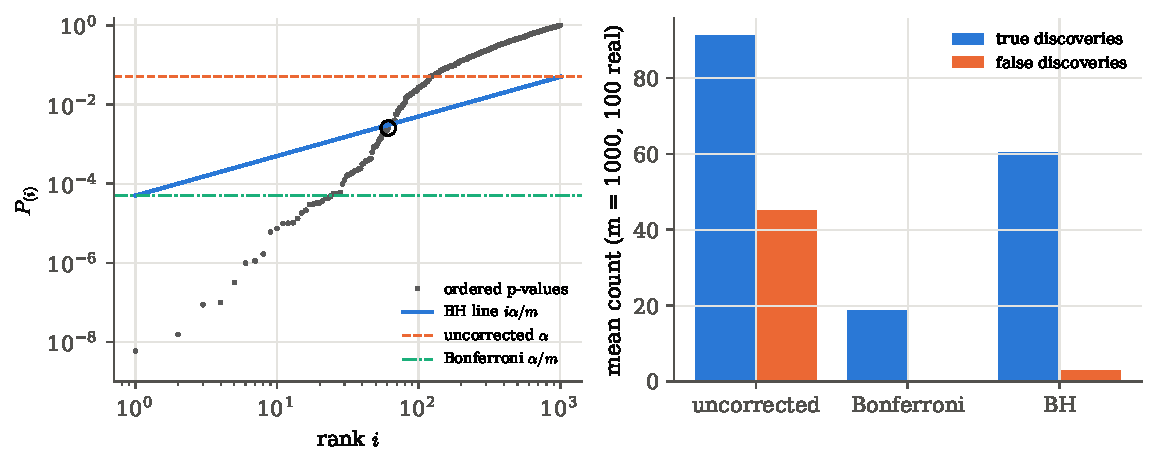
\includegraphics[width=\linewidth]{figures/ch04/bh_procedure.pdf}
\caption{Left: the thousand p-values of one simulated family, sorted, on
logarithmic axes. The real effects make the steep tail at small rank. The BH
threshold is the last p-value below the sloping line $i\alpha/m$ (circled);
the horizontal lines are the uncorrected and Bonferroni thresholds. Right: mean
numbers of true and false discoveries of the three procedures over $2000$
families.}
\label{4b:fig:bh}
\end{figure}

\begin{keyidea}[Two error rates for many tests]
The family-wise error rate $\Prob(V\ge1)$ is controlled by Bonferroni,
$P_i<\alpha/m$, for any dependence. The false discovery rate $\E(V/R)$ is
controlled by Benjamini--Hochberg, which rejects below the last crossing of
the line $i\alpha/m$. Use the first when a single false claim is costly (a
discovery), the second when a list of candidates will be followed up (a
screening).
\end{keyidea}

\subsection{The look-elsewhere effect in a mass scan}
\label{4b:sec:scan}

A resonance search is a multiple test with a continuum of tests: one for every
possible mass. (In this section $m$ is a mass, no longer a number of tests.)
\emph{What is done.} We do not know the mass, so for every hypothesised mass
$m$ we fit a signal of that mass and compute the likelihood-ratio statistic
$q_0(m)$ of the first part of the chapter. Its square root $Z(m)=\sqrt{q_0(m)}$
is the \newterm{local significance}, and $p_{\rm loc}=\Phi(-Z)$ the
\newterm{local p-value}. We then report the largest excess,
$q_{\max}=\max_mq_0(m)$.

\emph{Why the usual theory fails.} The mass exists only under the alternative:
with no signal, the background does not depend on $m$, so the null hypothesis
has no mass to fit. That is exactly the situation where Wilks' theorem does not
apply to the maximum \cite{GrossVitells2010}. \emph{The question} is then:
under the background-only hypothesis, how is the maximum over the scan
distributed?

\begin{workdef}[local and global p-value, trials factor]
The \newterm{local p-value} of the biggest bump is the probability, under the
background only, of an excess at least as large \emph{at its mass}. The
\newterm{global p-value} is the probability of an excess at least as large
\emph{anywhere in the search range}, $p_{\rm glob}=\Prob(q_{\max}\ge q_{\rm
obs}\given\Hnull)$. The \newterm{trials factor} is $p_{\rm glob}/p_{\rm loc}$.
\emph{Operational recipe:} simulate background-only data sets, scan each one
exactly as the data were scanned, record $q_{\max}$; $p_{\rm glob}$ is the
fraction with $q_{\max}\ge q_{\rm obs}$.
\end{workdef}

\paragraph{A simulated search.}
The script \pyname{code/ch04/17_bump_scan.py} generates a diphoton-like spectrum
of $\FourBScBtot$ background events in sixty $1\,$GeV bins from $100$ to
$160\,$GeV, falling exponentially with decay length $\FourBScSlope\,$GeV, and
searches for a Gaussian peak of width $\sigma_m=\FourBScSigM\,$GeV at
$\FourBScNmass$ masses between $105$ and $155\,$GeV in steps of $0.25\,$GeV. For
simplicity the background shape and normalisation are taken as known; in the
Gross--Vitells toy the normalisation is fitted, which changes the numbers, not
the method. At each mass the signal strength $\hat\mu\ge0$ maximises the binned
Poisson likelihood, and
\begin{equation}
  q_0(m)=2\Bigl[\sum_i n_i\ln\frac{b_i+\hat\mu s_i(m)}{b_i}-\hat\mu\Bigr],
  \qquad \hat\mu\ge0,
  \label{4b:eq:q0-scan}
\end{equation}
where $s_i(m)$ is the fraction of a unit signal at mass $m$ falling in bin $i$,
so that $\hat\mu$ counts signal events and $\sum_is_i=1$.

\pyfile[firstline=41,lastline=56,label={4b:lst:scan}]{code/ch04/17_bump_scan.py}{The scan: one-sided likelihood ratio at every mass, for many spectra at once}

The function takes a batch of spectra and returns $q_0$ at every mass for each
of them. \pyname{g0} is the slope of $\ln\Like$ at $\mu=0$. If it is negative,
the likelihood falls as soon as any signal is added, so the best non-negative
signal is zero and $q_0=0$. Otherwise Newton's method climbs the
log-likelihood, which is concave in $\mu$, starting from the linear estimate
$\sum s_i(n_i-b_i)/b_i\big/\sum s_i^2/b_i$; twelve iterations are plenty.
Arrays of shape (spectra, masses, bins) let numpy do all $500\times201$ fits of a
batch at once.

We took one background-only spectrum as ``the data'', choosing, among a
hundred generated ones, the spectrum whose largest local excess was closest to
$3\sigma$. \Cref{4b:fig:scan-spectrum} shows it. The best bump is at
$\FourBScMobs\,$GeV with $\hat\mu=\FourBScMuObs$ events, $q_0=\FourBScQobs$, local
significance $Z_{\rm loc}=\FourBScZloc$ and local p-value
$p_{\rm loc}=\FourBScPloc$. There is, of course, no particle.

\begin{figure}[htbp]
\centering
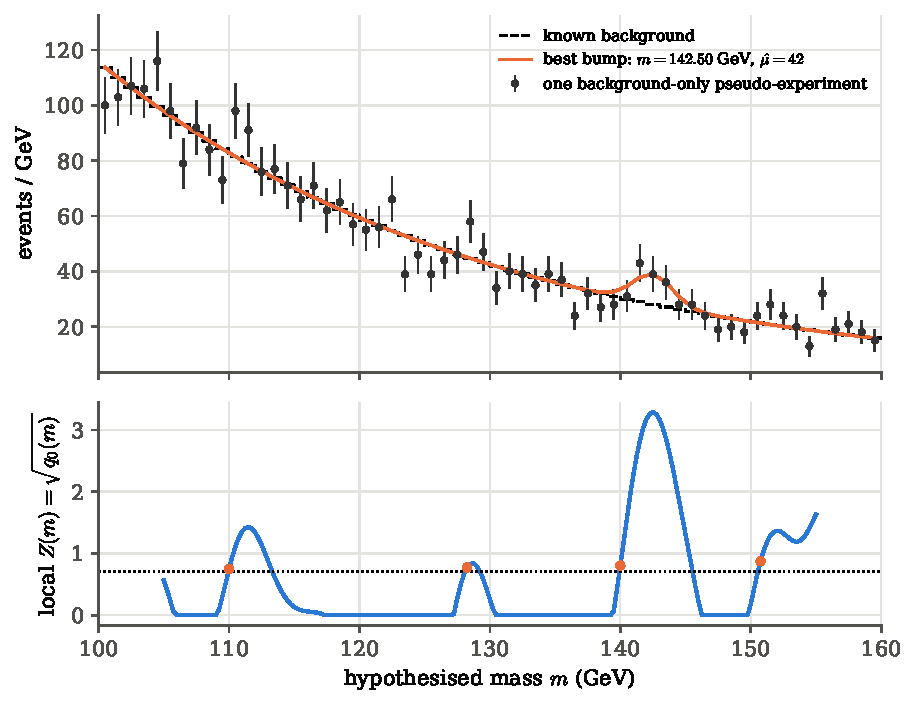
\includegraphics[width=0.85\linewidth]{figures/ch04/scan_spectrum.pdf}
\caption{Top: a background-only pseudo-experiment (points), the known
background (dashed) and the best fitted bump (orange). Bottom: the local
significance $\sqrt{q_0}$ as a function of the hypothesised mass. It is zero
wherever the data dip below the background, and the fluctuations are about as
wide as the mass resolution. The dotted line is the reference level
$\sqrt{0.5}$ used to count upcrossings (orange dots).}
\label{4b:fig:scan-spectrum}
\end{figure}

\emph{At one fixed mass} the results of the first part of the chapter still
hold. At $125\,$GeV, over $\FourBScToys$ background-only spectra, $q_0=0$ in
$\FourBScFracZero$ of them (the half-$\chi^2$ spike at zero) and
$\Prob(q_0>4)=\FourBScPfourMC$, against $\Phi(-2)=\FourBScPfourTh$. \emph{Over
all masses} the picture changes: a fraction $\FourBScPglob\pm\FourBScPglobErr$ of the
background-only spectra have $q_{\max}\ge\FourBScQobs$. So
\[
  p_{\rm loc}=\FourBScPloc\ (Z_{\rm loc}=\FourBScZloc),
  \qquad
  p_{\rm glob}=\FourBScPglob\ (Z_{\rm glob}=\FourBScZglob),
  \qquad
  \text{trials factor}\approx\FourBScTrials .
\]
A ``$\FourBScZloc\sigma$ bump'' is a $\FourBScZglob\sigma$ effect once we remember where we looked.
A local $3\sigma$ excess somewhere in this range appears in
$\FourBScPthreeGlob$ of background-only spectra, one in twenty-five.

\subsection{The global p-value without a million toys}
\label{4b:sec:gross-vitells}

The simulation needed $\FourBScToys$ scans to measure a global p-value of
$\FourBScPglob$. For a $5\sigma$ claim, $p\approx3\times10^{-7}$, it would need of order
$10^7$ scans, each a full fit \cite{GrossVitells2010}. Gross and Vitells, building
on a bound by Davies, found a way around this.

\emph{The event.} The largest excess is above some level $c$: $q_{\max}>c$.
\emph{How can it happen?} There are only two ways. Either $q_0$ is already
above $c$ at the lower end of the range, $m_{\rm lo}$, or $q_0(m)$ crosses the
level $c$ upwards at least once somewhere in the scan. Call $N(c)$ the number
of such \newterm{upcrossings}. Then
\begin{align}
  \Prob(q_{\max}>c)
  &\relby{1}{\le} \Prob\bigl(q_0(m_{\rm lo})>c\bigr)+\Prob\bigl(N(c)\ge1\bigr)
   \relby{2}{\le} p_{\rm loc}(c)+\E[N(c)] ,
  \label{4b:eq:davies}
\end{align}
\begin{explain}
  \item The union bound over the two ways of exceeding $c$.
  \item $\Prob(N\ge1)=\sum_{k\ge1}\Prob(N=k)\le\sum_kk\Prob(N=k)=\E N$; the
        first term is the local p-value at a fixed mass.
\end{explain}
and for large $c$ the bound becomes an equality, since two upcrossings of a high
level are rare \cite[(1)]{GrossVitells2010}. \emph{The remaining question:} how
does $\E[N(c)]$ depend on $c$? Treat $Z(m)$ as a smooth Gaussian process of
unit variance, a random curve along the mass axis. The rate at which it
crosses a level $u$ upwards is proportional to the density of $Z$ at $u$, that
is to $e^{-u^2/2}$ (Rice's formula). The proportionality constant depends on
how quickly $Z(m)$ forgets its value as $m$ changes, here on the mass
resolution, but not on $u$. With $q_0=Z^2$ and $u=\sqrt c$, this gives
$\E[N(c)]\propto e^{-c/2}$. So a count of upcrossings at one low reference
level $c_0$ fixes the whole curve \cite[(3)]{GrossVitells2010}:
\begin{equation}
  p_{\rm glob}(c)\ \approx\ p_{\rm loc}(c)+\E[N(c_0)]\,e^{-(c-c_0)/2}.
  \label{4b:eq:gv}
\end{equation}
At a low level upcrossings are frequent, so a handful of background-only
scans measures $\E[N(c_0)]$ well. With $c_0=0.5$ and only the first $100$ toys
we count $\E[N(c_0)]=\FourBScNzeroHundred$ (all $\FourBScToys$ give
$\FourBScNzeroAll$), and \eqref{4b:eq:gv} at $c=\FourBScQobs$ gives
$p_{\rm glob}\approx\FourBScPgv$, against $\FourBScPglob\pm\FourBScPglobErr$ from
the full simulation. \Cref{4b:fig:scan-tail} (left) compares the whole curves.

\paragraph{The trials factor grows with the significance.}
Divide \eqref{4b:eq:gv} by $p_{\rm loc}=\Phi(-Z)$, with $c=Z^2$, and use the
large-$Z$ tail estimate $\Phi(-Z)\approx e^{-Z^2/2}/(\sqrt{2\pi}\,Z)$ from the
first part of the chapter. Writing $\mathcal N_1=\E[N(c_0)]e^{c_0/2}$, so that
$\E[N(c)]=\mathcal N_1e^{-c/2}$,
\begin{align}
  \frac{p_{\rm glob}}{p_{\rm loc}}
  &\eqby{1} 1+\frac{\mathcal N_1e^{-Z^2/2}}{\Phi(-Z)}
   \relby{2}{\approx} 1+\mathcal N_1e^{-Z^2/2}\cdot\sqrt{2\pi}\,Z\,e^{Z^2/2}
   \eqby{3} 1+\sqrt{2\pi}\,\mathcal N_1Z .
  \label{4b:eq:trials}
\end{align}
\begin{explain}
  \item Divide \eqref{4b:eq:gv} by $p_{\rm loc}$ and insert $c=Z^2$.
  \item The Gaussian tail estimate.
  \item The exponentials cancel.
\end{explain}
The trials factor is not a fixed ``number of independent masses''. It grows
linearly with the local significance \cite[(12)]{GrossVitells2010}. (Gross and
Vitells write $1+\sqrt{\pi/2}\,\mathcal NZ$ for the two-sided statistic, whose
level crossings are twice as many, $\mathcal N=2\mathcal N_1$: the same formula.)
Here $\mathcal N_1=\FourBScNone$, so a local $3\sigma$ bump carries a trials
factor of about $\FourBScTrialsThreeAsym$ and our $\FourBScZloc\sigma$ bump about $\FourBScTrials$,
matching the toys (\cref{4b:fig:scan-tail}, right). \emph{Why does it grow?}
A higher level is crossed only near the top of a fluctuation, and the part of
the fluctuation above the level gets narrower as the level rises. A pre-chosen
mass must land on that narrow top, so the local p-value falls faster than the
chance that the top appears somewhere in the range. For a local
$5\sigma$ excess in this search, \eqref{4b:eq:gv} gives
$p_{\rm glob}=\FourBScPgvFive$, a global significance of $\FourBScZgvFive\sigma$,
from $p_{\rm loc}=\FourBScPlocFive$: no simulation of $10^7$ scans needed.

\begin{figure}[htbp]
\centering
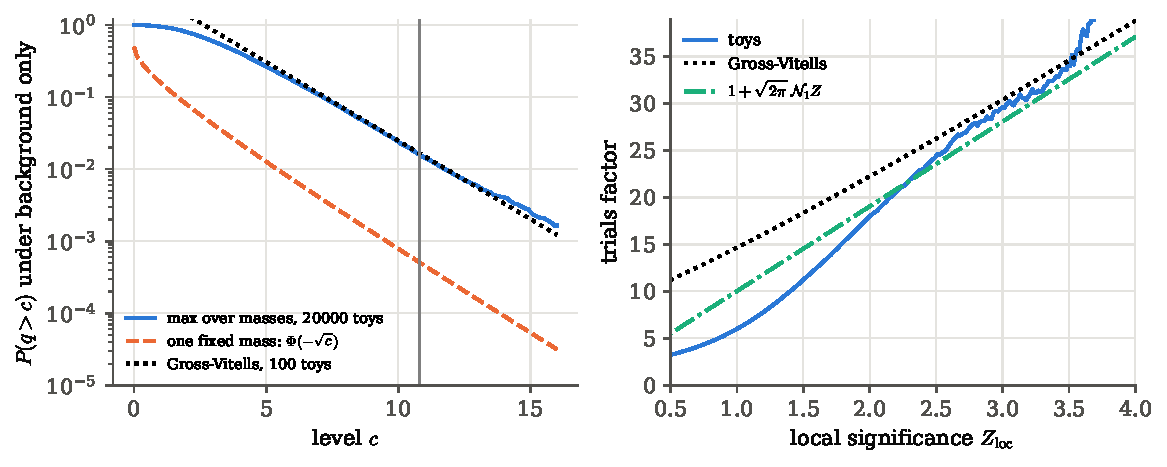
\includegraphics[width=\linewidth]{figures/ch04/scan_tail.pdf}
\caption{Left: the probability, with background only, that the largest excess
exceeds a level $c$ anywhere in the scan (blue, $20\,000$ toys), compared with
the local probability at one fixed mass (orange dashed) and the Gross--Vitells
formula calibrated on $100$ toys (black dotted). The vertical line marks the
observed bump. Right: the trials factor, global over local p-value, as a
function of the local significance, with the Gross--Vitells prediction and its
asymptotic straight line.}
\label{4b:fig:scan-tail}
\end{figure}

\paragraph{What ``elsewhere'' means.}
The global p-value refers to the range of the scan, and that range must be
fixed before the data are seen. But other decay channels, other signal widths
and other analyses in the same experiment are also places one could have
looked. There is no unique answer to how far ``elsewhere'' extends. That is why
experiments quote the local significance together with the global one for a
stated range.

\begin{inpractice}[How searches report the look-elsewhere effect]
A search at a collider quotes the local p-value of the largest excess, and a
global p-value over a stated mass range, obtained from background-only toys
where affordable and from the upcrossing formula \eqref{4b:eq:gv} otherwise. The
test statistic is the profile likelihood ratio of \cite{Cowan2011} with the
nuisance parameters (background shape, energy scale) fitted in every toy. The
same formula applies to any scan over a parameter that exists only under the
signal hypothesis: the position of a localised feature in the CMB power
spectrum, the frequency of an oscillation in a Galactic-centre spectrum, the
sky position and frequency of a gravitational-wave template.
\end{inpractice}

The Bayesian language of \cref{ch:05} handles the same problem differently.
The unknown mass gets a prior spread over the search range. The evidence for a
signal is then automatically diluted by the fraction of the range that is
compatible with the bump. This dilution, the \emph{Occam factor}, plays the
role of the trials factor.

Two things were held simple in this scan: the background shape was known, and
the only question was discovery. A real search fits the background together
with its systematic uncertainties, and when nothing is found it must say which
signal strengths are excluded. \Cref{4b:sec:templates} builds the likelihood
with nuisance parameters that the scan's $q_0(m)$ then uses, and
\cref{4b:sec:limits} turns the same profile likelihood ratio into upper limits,
$\mathrm{CL}_s$ and the expected band.
\section{A search as a likelihood: templates and nuisance parameters}
\label{4b:sec:templates}

In the summer of 2012 two experiments at the LHC showed the same kind of plot: a
histogram of the invariant mass of photon pairs, a smooth background falling from
left to right, and a small bump near $125\,$GeV. The question put to that histogram
was simple to say. Is there a signal in it, and how big is it? The size is quoted
as a \newterm{signal strength} $\mu$ \unpack{the number of signal events seen,
divided by the number the Standard Model predicts}, so $\mu=0$ means ``background
only'' and $\mu=1$ means ``the predicted Higgs boson''.

But the number of signal events the Standard Model ``predicts'' in that histogram is
not known exactly. It depends on how many collisions were recorded (the luminosity),
on how often a real photon pair passes the selection (the efficiency), and on where
exactly a $125\,$GeV peak lands on the measured mass axis (the photon energy scale).
Each of these was measured in a separate calibration, each to a few per cent. The
background level under the peak is not predicted at all; it has to be read off the
data. So the honest statement of the experiment's knowledge is not one number for
the prediction but a prediction that depends on several uncertain inputs, each of
which has been measured somewhere. Writing all of that as one likelihood is what
turns a histogram into a measurement of $\mu$, and the same construction serves
any search: a dark-matter recoil spectrum, a line in an X-ray spectrum, an excess of
gravitational-wave triggers above the noise.

\paragraph{The question in words.}
\begin{enumerate}[label=\arabic*.]
  \item What is the probability of the whole histogram, given a signal strength and
        everything else the prediction depends on?
  \item What is a ``systematic uncertainty'' in this language, and why does it
        become a parameter with a measurement of its own?
  \item How do we remove those extra parameters to speak about $\mu$ alone, and how
        does this compare with the profile likelihood of \cref{ch:03} and with the
        Bayesian marginalisation of \cref{ch:05}?
\end{enumerate}

\subsection{The probability of a histogram}
\label{4b:sec:binned-like}

Start with what is recorded. Each selected event has a measured mass $x$, and the
events are sorted into bins, $n_1,\dots,n_N$ events in bins $1,\dots,N$. What is the
probability of this list of counts?

\emph{The inputs.} Two physical assumptions carry everything, the same ones that
gave the Poisson distribution in \cref{ch:02}: the collisions that produce
selected events happen independently of each other, one at a time, and at a rate
that does not change during the run. Then the total number of selected events $N_{\rm tot}$
is Poisson with some mean $\nu_{\rm tot}$. One more input, also physical: each event
lands in bin $i$ with a probability $p_i$ that does not depend on the other events.

\emph{The question:} the bins split one Poisson stream into $N$ pieces; what is the
joint probability of the counts in the pieces? Given the total, the counts are
multinomial (each of the $N_{\rm tot}$ events chooses its bin independently). So,
with $N_{\rm tot}=\sum_in_i$ and $\nu_i=\nu_{\rm tot}p_i$,
\begin{align}
  \Prob(n_1,\dots,n_N)
  &\eqby{1} \Prob(N_{\rm tot})\,\Prob(n_1,\dots,n_N\given N_{\rm tot})
   \eqby{2} \frac{\nu_{\rm tot}^{N_{\rm tot}}e^{-\nu_{\rm tot}}}{N_{\rm tot}!}\,
            \frac{N_{\rm tot}!}{n_1!\cdots n_N!}\,p_1^{n_1}\cdots p_N^{n_N}
  \notag\\
  &\eqby{3} \prod_{i=1}^N\frac{(\nu_{\rm tot}p_i)^{n_i}}{n_i!}\,e^{-\nu_{\rm tot}p_i}
   \eqby{4} \prod_{i=1}^N\frac{\nu_i^{n_i}}{n_i!}\,e^{-\nu_i} .
  \label{4b:eq:split}
\end{align}
\begin{explain}
  \item The product rule: first the total, then how it is shared among the bins.
  \item Poisson for the total; multinomial for the sharing.
  \item The $N_{\rm tot}!$ cancel; write $\nu_{\rm tot}^{N_{\rm tot}}=\prod_i\nu_{\rm tot}^{n_i}$
        and $e^{-\nu_{\rm tot}}=\prod_ie^{-\nu_{\rm tot}p_i}$, using $\sum_in_i=N_{\rm tot}$
        and $\sum_ip_i=1$.
  \item Name the mean of bin $i$, $\nu_i=\nu_{\rm tot}p_i$.
\end{explain}
The joint probability factorises: the bin counts are \emph{independent} Poisson
variables, each with its own mean. Nothing about the bins being ``far apart'' was
needed; the independence comes from the Poisson total.

\emph{Signal plus background.} In each bin the events come from two independent
sources, signal and background. The sum of two independent Poisson counts is Poisson
with the summed mean (\cref{ch:02}), so the mean of bin $i$ is
\begin{equation}
  \nu_i=\mu\,s_i+b_i,
  \qquad
  s_i=S\,f_i,\quad b_i=B\,g_i .
  \label{4b:eq:nu-template}
\end{equation}
Here $S$ and $B$ are the expected total numbers of signal (for $\mu=1$) and
background events, and $f_i$, $g_i$ are the fractions of each falling in bin $i$
\cite[(2)--(4)]{Cowan2011}.

\begin{workdef}[template]
A \newterm{template} is the predicted histogram of one process: the fractions $f_i$
(signal) or $g_i$ (background) of its events expected in each bin \unpack{a shape,
normalised to one, usually made by running the detector simulation on many simulated
events}. The analysis fits the data as a sum of templates with free or constrained
normalisations. \emph{Operationally:} histogram the simulated events of each process
with the binning of the data, divide by their number.
\end{workdef}

\paragraph{Example: the search we will follow.}
Our pseudo-experiment has sixty $1\,$GeV
bins from $100$ to $160\,$GeV. The background template $g_i$ is a falling exponential
of decay length $\FourBTpSlope\,$GeV with $B=\FourBTpBtot$ expected events; the signal
template $f_i$ is a Gaussian peak at $125\,$GeV with the mass resolution
$\sigma_m=\FourBTpSigM\,$GeV and $S=\FourBTpSzero$ expected events. The data were
generated with $\mu=1$ by the library \pyname{code/ch04/lib_templates.py}. With every input known, the likelihood would be
\eqref{4b:eq:split} with \eqref{4b:eq:nu-template} inserted, a function of $\mu$
alone, exactly the likelihood that was scanned over masses in \cref{4b:sec:scan}.

\subsection{Systematic uncertainties become nuisance parameters}
\label{4b:sec:nuisance-hep}

Now let the inputs be uncertain, as they are. Take the three of our example one at a
time, and ask of each: \emph{how does it change the predicted counts, and who
measured it?}
\begin{itemize}[itemsep=1pt,leftmargin=1.2em]
  \item \emph{The background normalisation} $\beta$. The background is $\beta B$
        instead of $B$. Nobody predicts $\beta$ well; the data measure it, from the
        bins away from the peak (the \newterm{sidebands}) or from a separate
        \newterm{control region} chosen to contain no signal.
  \item \emph{The signal yield} $\kappa$, luminosity times efficiency relative to its
        nominal value. The signal is $\mu\kappa S$ instead of $\mu S$. A calibration
        measured $\kappa$: its result was $a_\kappa=1$ with an error of
        $\sigma_\kappa=\FourBTpSigKappa$.
  \item \emph{The energy scale} $\delta$. A mis-calibration shifts every measured
        photon energy, so the peak sits at $125+\delta$ and the signal template
        becomes $f_i(125+\delta)$. The scale was calibrated on the well-known $Z$
        boson peak: $a_\delta=0$ with $\sigma_\delta=\FourBTpSigDelta\,$GeV.
\end{itemize}
Each of these is a parameter the predicted counts depend on and that we do not want
to report: a \newterm{nuisance parameter} (\cref{ch:03}). The first one is
different from the other two in kind. It changes the background, which the
histogram itself measures. The other two change the signal, which the histogram
cannot separate from $\mu$: a larger $\kappa$ and a smaller $\mu$ give the same peak.
Only the calibration can tell them apart.

\emph{What should be done with $\kappa$?} There are three candidates. We could fix it
at $1$; that pretends the calibration was perfect, and \cref{ch:03} showed what this
costs: intervals too short by the factor $\sqrt{1-\rho^2}$ and coverage below its
promise. We could leave it free with no information; then $\mu$ and $\kappa$ are
completely degenerate and $\mu$ is not measured at all. Or we could use what the
calibration actually found. The calibration is a measurement like any other. Its
result $a_\kappa$ is a random number whose distribution depends on the true
$\kappa$: Gaussian, with mean $\kappa$ and standard deviation $\sigma_\kappa$. The
probability of the calibration result, read as a function of $\kappa$, is its
likelihood. The calibration and the search are independent measurements, so the
probability of both results is the product of their probabilities. This gives the
complete likelihood
\begin{equation}
  \Like(\mu,\bm\theta)
  =\prod_{i=1}^{N}\frac{\bigl(\mu\,s_i(\bm\theta)+b_i(\bm\theta)\bigr)^{n_i}}{n_i!}\,
     e^{-(\mu s_i(\bm\theta)+b_i(\bm\theta))}
   \;\times\;\prod_{k}p\bigl(a_k\given\theta_k\bigr) ,
  \label{4b:eq:full-like}
\end{equation}
with $\bm\theta=(\beta,\kappa,\delta)$ the nuisance parameters and one factor
$p(a_k\given\theta_k)$ for each auxiliary measurement \cite[(6)]{Cowan2011},
\cite{Cranmer2015}. For a calibration quoted as $a_k\pm\sigma_k$,
\begin{equation}
  p(a_k\given\theta_k)=\frac{1}{\sqrt{2\pi}\,\sigma_k}\,
  \exp\Bigl[-\frac{(a_k-\theta_k)^2}{2\sigma_k^2}\Bigr],
  \label{4b:eq:constraint}
\end{equation}
a \newterm{constraint term}. If the auxiliary measurement is itself a count, a
control region with $m$ events expected to be $\tau\beta B$, the factor is Poisson
instead; \cref{4b:sec:onoff-hep} works that case out.

\begin{pitfall}[A constraint term is a likelihood, not a prior]
The Gaussian factor \eqref{4b:eq:constraint} looks like a prior on $\theta_k$, and in a
Bayesian analysis it is combined with one. But in \eqref{4b:eq:full-like} it is the
probability of an observed number, the calibration result $a_k$, given the
parameter. In pseudo-experiments, therefore, $a_k$ must be \emph{generated} afresh
together with the histogram (the calibration would have come out differently too),
not held at its observed value \cite{Cowan2011}.
\end{pitfall}

A nuisance parameter can change the \emph{shape} of a template, not only its size: the
energy scale moves the peak. Real analyses rarely have a formula like
$f_i(125+\delta)$. They have the nominal template and two shifted ones, made by
re-running the simulation with the calibration moved up and down by one standard
deviation, and they interpolate between them bin by bin \cite{Cranmer2015}. With
$\theta$ measured in units of its calibration error, the simplest choice is
\begin{equation}
  f_i(\theta)=f_i^{0}+\theta\,\bigl(f_i^{+}-f_i^{0}\bigr)\quad(\theta\ge0),
  \qquad
  f_i(\theta)=f_i^{0}+\theta\,\bigl(f_i^{0}-f_i^{-}\bigr)\quad(\theta<0),
  \label{4b:eq:morph}
\end{equation}
so that $\theta=0,\pm1$ give back the three simulated templates, and the constraint
term is a standard normal in $\theta$.

\Cref{4b:fig:like-structure} shows how the pieces of \eqref{4b:eq:full-like} hang
together: every parameter predicts some measurements, every measurement
contributes one factor, and the likelihood is their product.

\begin{figure}[htbp]
\centering
\begin{tikzpicture}[
  par/.style={draw=formblue,thick,rounded corners=2pt,inner sep=4pt,font=\small,fill=formblue!6},
  meas/.style={draw=fibreorange,thick,rounded corners=2pt,inner sep=4pt,font=\small,fill=fibreorange!6,align=center},
  arr/.style={->,>=stealth,thick,black!55}]
  \node[par] (mu) at (0,2.2) {$\mu$ signal strength};
  \node[par] (be) at (4.2,2.2) {$\beta$ background};
  \node[par] (ka) at (-4.2,2.2) {$\kappa$ signal yield};
  \node[par] (de) at (-4.2,0.9) {$\delta$ energy scale};
  \node[meas] (hist) at (0,-0.6) {mass histogram $n_i$\\[1pt]\footnotesize Poisson, mean $\mu\kappa S f_i(125+\delta)+\beta B g_i$};
  \node[meas] (ak) at (-5.0,-2.3) {calibration $a_\kappa$\\[1pt]\footnotesize Gaussian, mean $\kappa$};
  \node[meas] (ad) at (-1.7,-2.3) {$Z$-peak scale $a_\delta$\\[1pt]\footnotesize Gaussian, mean $\delta$};
  \node[meas] (cr) at (3.6,-2.3) {control region $m$\\[1pt]\footnotesize Poisson, mean $\tau\beta B$};
  \draw[arr] (mu) -- (hist);
  \draw[arr] (be) -- (hist);
  \draw[arr] (ka) -- (hist);
  \draw[arr] (de) -- (hist);
  \draw[arr] (ka.west) to[out=200,in=100] (ak.north);
  \draw[arr] (de.south) to[out=-80,in=90] (ad.north);
  \draw[arr] (be.east) to[out=-20,in=60] (cr.north east);
\end{tikzpicture}
\caption{The structure of a search likelihood. Parameters (blue) predict the
measurements (orange). The signal strength $\mu$ is predicted only by the main
histogram, where it always appears multiplied by the signal yield $\kappa$; the
calibrations measure $\kappa$ and the energy scale $\delta$ on their own, and the
background normalisation $\beta$ is measured by the histogram's sidebands and,
optionally, by a control region. The likelihood is the product of one factor per
measurement.}
\label{4b:fig:like-structure}
\end{figure}

\subsection{Removing the nuisance parameters: fix, profile or integrate}
\label{4b:sec:profile-hep}

We have met this problem twice before, and it is worth recalling both times
concretely. In \cref{ch:03}, in the section on nuisance parameters and the profile
likelihood, a counting experiment saw $\ThreeBProfNon$ events in a signal region and
$\ThreeBProfNoff$ in a control region of the same size. The estimated signal was
$\hat s=\ThreeBProfS$. Holding the background fixed at its best value gave the error
$^{+\ThreeBCondHi}_{-\ThreeBCondLo}$, letting it adjust (profiling) gave
$^{+\ThreeBProfHi}_{-\ThreeBProfLo}$, and in simulated repetitions only the profile
interval covered the truth $68\%$ of the time ($\ThreeBProfCover$ against
$\ThreeBCondCover$). In \cref{ch:05}, in the section on nuisance parameters, the
Bayesian removed a background level by integrating the joint posterior over it, and
found that integrating and maximising agree when the likelihood is Gaussian, and
differ by a ``volume'' factor (how many values of the nuisance parameter fit almost as
well) when it is not. The search likelihood \eqref{4b:eq:full-like} is the same
problem with three differences: there are several nuisance parameters, their
information comes from separate auxiliary measurements, and the goal is not only an
interval but the test statistics of \cref{4b:sec:limits}.

The frequentist tool is the same as in \cref{ch:03}: the \newterm{profile likelihood
ratio}
\begin{equation}
  \lambda(\mu)=\frac{\Like\bigl(\mu,\hat{\hat{\bm\theta}}(\mu)\bigr)}{\Like(\hat\mu,\hat{\bm\theta})},
  \qquad 0\le\lambda(\mu)\le1,
  \label{4b:eq:lambda}
\end{equation}
where $\hat\mu,\hat{\bm\theta}$ maximise $\Like$ over everything, and
$\hat{\hat{\bm\theta}}(\mu)$ maximises it over the nuisance parameters with $\mu$ held
fixed \cite[(7)]{Cowan2011}. The double hat is read ``the best nuisance parameters
for this $\mu$''. The numerator can never exceed the denominator, because the
denominator is maximised over more.

Set the three ways of removing $\bm\theta$ side by side.
\begin{itemize}[itemsep=1pt,leftmargin=1.2em]
  \item \emph{Fix} $\bm\theta$ at $\hat{\bm\theta}$: the conditional likelihood. It
        keeps only the statistical fluctuation of the histogram. Its width is the
        ``statistical error''.
  \item \emph{Profile}: at each $\mu$, let $\bm\theta$ take its best value. The
        width of $-2\ln\lambda(\mu)$ is the total error.
  \item \emph{Integrate}: give $\bm\theta$ a prior (here flat in $\beta$, and the
        calibrations' Gaussians, which are then genuinely priors) and integrate the
        joint posterior over it, as in \cref{ch:05}.
\end{itemize}
\emph{What is the same?} For a Gaussian likelihood all three are Gaussians in $\mu$;
profiling and integrating give the same width, the full variance $V_{\mu\mu}$, and
fixing gives the smaller $1/F_{\mu\mu}$ (\cref{ch:03}). \emph{What differs?} The
meaning: the profile curve is a likelihood ratio whose sampling distribution we will
compute, the marginal is a posterior density that needs a prior. And the shape, as
soon as the likelihood is not Gaussian, through the volume factor.

\emph{How large is the systematic part of the error?} Analyses quote it separately,
by subtraction. For one nuisance parameter, \cref{ch:03} found
$1/F_{\mu\mu}=V_{\mu\mu}(1-\rho^2)$, with $\rho$ the correlation of $\hat\mu$ and
$\hat\theta$, so
\begin{equation}
  \sigma_{\rm syst}^2
  \equiv\sigma_{\rm tot}^2-\sigma_{\rm stat}^2
  \eqby{1} V_{\mu\mu}-\frac{1}{F_{\mu\mu}}
  \eqby{2} V_{\mu\mu}-V_{\mu\mu}(1-\rho^2)
  =\rho^2\,V_{\mu\mu} .
  \label{4b:eq:syst}
\end{equation}
\begin{explain}
  \item The profile width is $\sqrt{V_{\mu\mu}}$, the conditional width $\sqrt{1/F_{\mu\mu}}$.
  \item The identity of \cref{ch:03}.
\end{explain}
The ``systematic error'' is the part of the variance of $\hat\mu$ that it shares with
the nuisance parameter through their correlation. It adds to the statistical one in
quadrature by construction, not by assumption. With several nuisance parameters the
same subtraction is used, and $\rho^2$ becomes the fraction of the variance of
$\hat\mu$ that all of them together account for.

\paragraph{Example: the template fit.}
The script \pyname{code/ch04/19_hep_templates.py} maximises \eqref{4b:eq:full-like}
for our pseudo-data. The heart of it is the negative log-likelihood:

\pyfile[firstline=33,lastline=46,label={4b:lst:nll}]{code/ch04/lib_templates.py}{The search likelihood: Poisson bins times two Gaussian constraint terms}

\pyname{expected} builds the mean counts \eqref{4b:eq:nu-template} with the three
nuisance parameters inserted; \pyname{nll} returns $-\ln\Like$ without the constants
$\ln n_i!$ and $\ln\sqrt{2\pi}\sigma_k$, which cancel in every ratio. A numerical
minimiser (\pyname{scipy.optimize.minimize}) does the rest, over all four parameters
for the denominator of \eqref{4b:eq:lambda}, over the three nuisance parameters at
each fixed $\mu$ for the numerator. The global fit gives
\[
  \hat\mu=\FourBTpMuHat,\qquad
  \hat\beta=\FourBTpBetaHat,\qquad
  \hat\kappa=\FourBTpKappaHat,\qquad
  \hat\delta=\FourBTpDeltaHat\,\text{GeV}.
\]
Why is $\hat\kappa$ exactly the calibration value? Because the histogram sees only the
product $\mu\kappa$. Whatever the product the histogram prefers, the fit can reach it
with any $\kappa$ by moving $\mu$, so it sets $\kappa$ where its own measurement, the
calibration, wants it. The energy scale, in contrast, is pulled a little by the data:
the peak in the histogram sits slightly below $125\,$GeV, and the fit moves it by a
fraction of the calibration error.

\Cref{4b:fig:templates} (right) shows the three curves. Read at
$-2\ln(\Like/\Like_{\max})=1$:
\[
  \text{fixed: }\hat\mu^{+\FourBTpCondHi}_{-\FourBTpCondLo},
  \qquad
  \text{profile: }\hat\mu^{+\FourBTpProfHi}_{-\FourBTpProfLo},
  \qquad
  \text{marginal: }\FourBTpMargMode^{+\FourBTpMargHi}_{-\FourBTpMargLo}.
\]
So $\sigma_{\rm stat}=\FourBTpSigStat$, $\sigma_{\rm tot}=\FourBTpSigTot$, and by
\eqref{4b:eq:syst} $\sigma_{\rm syst}=\FourBTpSigSyst$. Most of the systematic part is the
$10\%$ yield calibration: since the histogram measures $\mu\kappa$, a $10\%$ error on
$\kappa$ is a $10\%$ error on $\mu$, about $0.1\,\hat\mu\approx0.11$, and
$\sqrt{\FourBTpSigStat^2+0.11^2}\approx0.33$. Profiling and marginalising nearly agree: the marginal peaks slightly lower, at
$\FourBTpMargMode$, with almost the same width, and the largest difference between the two curves inside the
plotted interval is $\FourBTpMaxDiffPM$ in $-2\ln$. That is the volume effect of
\cref{ch:05} at work, small here because the likelihood is close to Gaussian. The
sizes are the lesson. A $1.5\,$GeV resolution and $\FourBTpBtot$ background events make
the statistical error dominant; a ten times larger data set would shrink
$\sigma_{\rm stat}$ by $\sqrt{10}$ and leave $\sigma_{\rm syst}$ untouched, and the
calibration would then limit the measurement.

\begin{figure}[htbp]
\centering
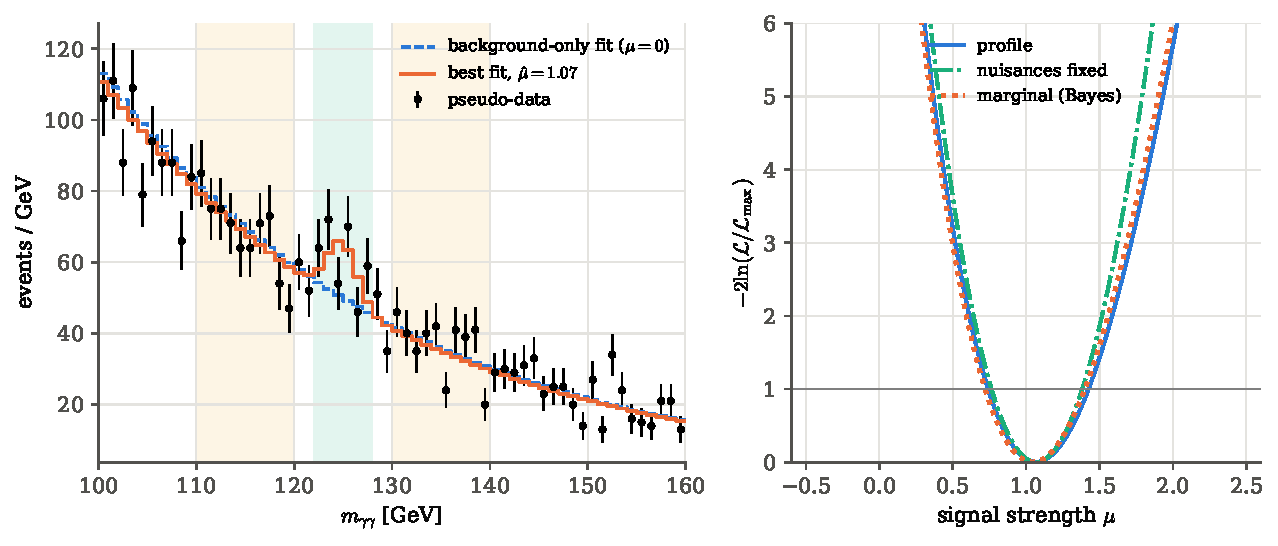
\includegraphics[width=\linewidth]{figures/ch04/hep_templates.pdf}
\caption{Left: the pseudo-data (points), the best background-only fit (blue dashed)
and the best signal-plus-background fit (orange). The green band is the signal
window and the yellow bands the sidebands used by the counting version of the search.
Right: three ways of turning the four-parameter likelihood into a curve for $\mu$.
Fixing the nuisance parameters gives the narrowest curve (the statistical error);
profiling them gives the total error; integrating them with priors (Bayes) gives
nearly the same curve, slightly shifted towards smaller $\mu$. The grey line at
one marks the $68\%$ interval.}
\label{4b:fig:templates}
\end{figure}

\subsection{The smallest search: a signal window and its sidebands}
\label{4b:sec:onoff-hep}

Every piece of the template likelihood can be seen working, and solved by hand, in a
stripped-down version of the same search. Keep only two numbers from the histogram:
the count $n$ in a signal window around the peak, $122$--$128\,$GeV, and the count
$m$ in two sidebands, $110$--$120$ and $130$--$140\,$GeV (\cref{4b:fig:templates},
left). In the window we expect $\mu s+b$ events, where $s=\FourBTpSwin$ is the
nominal signal falling in the window and $b$ the unknown background. In the
sidebands we expect $\tau b$, where $\tau=\FourBTpTau$ is the ratio of the background
template integrated over the sidebands to its integral over the window. The shape is
taken as known; only its normalisation $b$ is not. The sidebands are the control
region and $b$ is the nuisance parameter. The likelihood is two Poisson factors
\cite[(90)]{Cowan2011},
\begin{equation}
  \ln\Like(\mu,b)=n\ln(\mu s+b)-(\mu s+b)+m\ln(\tau b)-\tau b+\text{const},
  \label{4b:eq:onoff}
\end{equation}
the on/off likelihood of \cref{ch:03} with $k$ renamed $\tau$ and the signal written
as $\mu s$.

\emph{The global maximum.} Setting the two derivatives to zero,
\begin{align}
  \frac{\partial\ln\Like}{\partial\mu}
  &\eqby{1} s\Bigl(\frac{n}{\mu s+b}-1\Bigr)=0
   \;\Rightarrow\; \hat\mu s+\hat b=n,
  \notag\\
  \frac{\partial\ln\Like}{\partial b}
  &\eqby{2} \frac{n}{\mu s+b}-1+\frac{m}{b}-\tau=0
   \;\Rightarrow\;\hat b=\frac{m}{\tau},
   \qquad \hat\mu=\frac{n-m/\tau}{s} .
  \label{4b:eq:onoff-mle}
\end{align}
\begin{explain}
  \item Only the first two terms of \eqref{4b:eq:onoff} contain $\mu$.
  \item By the first equation the first two terms cancel, leaving $m/b=\tau$; then
        $\hat\mu s=n-\hat b$.
\end{explain}
In words: the sidebands estimate the background, scaled down to the window by $\tau$,
and the signal is what is left over. With $n=\FourBTpNon$ and $m=\FourBTpNoff$,
$\hat b=\FourBTpBhatOO$ and $\hat\mu=\FourBTpMuOO$. We allow $\hat\mu<0$ here: it is
whatever value maximises the likelihood, as long as the mean count $\mu s+b$ stays
positive. \Cref{4b:sec:limits} needs this.

\emph{The best background for a given $\mu$.} Hold $\mu$ fixed and solve only the
second equation of \eqref{4b:eq:onoff-mle}:
\begin{align}
  0&\eqby{1} n\,b-b(\mu s+b)+m(\mu s+b)-\tau b(\mu s+b)
  \notag\\
   &\eqby{2} -(1+\tau)\,b^2+\bigl[n+m-(1+\tau)\mu s\bigr]\,b+m\mu s ,
  \notag\\
  \hat{\hat b}(\mu)
  &\eqby{3} \frac{A}{2(1+\tau)}+\sqrt{\frac{A^2+4(1+\tau)\,m\,\mu s}{4(1+\tau)^2}},
  \qquad A=n+m-(1+\tau)\mu s .
  \label{4b:eq:bhh}
\end{align}
\begin{explain}
  \item Multiply $\partial\ln\Like/\partial b=0$ by $b(\mu s+b)>0$.
  \item Collect powers of $b$.
  \item The quadratic formula; for $\mu>0$ the constant term $m\mu s$ is positive, so
        the roots have opposite signs and only the $+$ root is a background.
\end{explain}
This is \cite[(93)]{Cowan2011}, and the same quadratic as in \cref{ch:03}. At $\mu=0$
the square root equals $A/(2(1+\tau))$ and
$\hat{\hat b}(0)=(n+m)/(1+\tau)$: with no signal, the window and the sidebands are
pooled into one background measurement. Here $\hat{\hat b}(0)=\FourBTpBhhOO$, more
than $\hat b$, because the pooled estimate also uses the excess in the window.

\emph{The discovery statistic.} For $\hat\mu>0$, $q_0=-2\ln\lambda(0)$. At the global
maximum $\hat\mu s+\hat b=n$ and $\tau\hat b=m$; at $\mu=0$ the window mean is
$\hat{\hat b}(0)$ and the sideband mean $\tau\hat{\hat b}(0)$, and the two linear
terms add up to $(1+\tau)\hat{\hat b}(0)=n+m$. So
\begin{align}
  q_0
  &\eqby{1} 2\Bigl[\bigl(n\ln n-n+m\ln m-m\bigr)
          -\bigl(n\ln\hat{\hat b}(0)+m\ln\tau\hat{\hat b}(0)-(n+m)\bigr)\Bigr]
  \notag\\
  &\eqby{2} 2\Bigl[n\ln\frac{n}{\hat{\hat b}(0)}+m\ln\frac{m}{\tau\,\hat{\hat b}(0)}\Bigr].
  \label{4b:eq:q0-onoff}
\end{align}
\begin{explain}
  \item \eqref{4b:eq:onoff} at the two maxima, using the values just listed.
  \item The $-(n+m)$ terms cancel; combine the logarithms.
\end{explain}
The numbers give $q_0=\FourBTpQzeroOO$, a significance $Z=\sqrt{q_0}=\FourBTpZOO$
(\cref{4b:sec:wald-asym} shows why the square root is the significance even with a
nuisance parameter). Compare with two neighbours.
\begin{itemize}[itemsep=1pt,leftmargin=1.2em]
  \item \emph{The background known exactly}, $b=\FourBTpBwin$: the formula of the first
        part of the chapter, $q_0=2[n\ln(n/b)-(n-b)]$, gives $Z=\FourBTpZKB$.
  \item \emph{The full template fit} of \cref{4b:sec:profile-hep}, with three nuisance
        parameters: $Z=\sqrt{q_0}=\FourBTpZzero$.
\end{itemize}
One pseudo-experiment is a poor judge of which method is better: all three values of
$Z$ move with the luck of the same data. The expected significances, computed with the
Asimov data set of \cref{4b:sec:asimov}, do not: $\FourBTpZAOO$ for the window with
sidebands, $\FourBTpZAKB$ with the background known, and $\FourBTpZA$ for the template
fit. Measuring the background instead of knowing it costs significance. The template
fit wins it back, because it uses every bin, each weighted by its own ratio of signal
to background, instead of a window with a hard edge.

The size of the cost is easiest to see in the Gaussian limit. $\hat\mu=(n-m/\tau)/s$ is
a difference of independent counts, so its variance is about
$(n+m/\tau^2)/s^2$, an error of $\FourBTpSigOO$; with the background known it would be
$\sqrt n/s=\FourBTpSigOOKB$. The control region adds the term $m/\tau^2\approx b/\tau$:
a control region $\tau$ times larger than the window adds a fraction $1/\tau$ of the
background variance.

The lesson in one line: a systematic uncertainty is a parameter with a measurement of
its own, and the search likelihood is the product of the main measurement and those
auxiliary measurements.

\section[Discovery and exclusion: $q_0$, $\tilde q_\mu$, CL$_s$, Brazil band]{Discovery and exclusion with nuisance parameters: $q_0$, $\tilde q_\mu$, CL$_s$ and the Brazil band}
\label{4b:sec:limits}

The discovery statistic $q_0$ has appeared twice already. In the first part of the
chapter, a count $N$ on a \emph{known} background $b$ gave
$q_0=2[N\ln(N/b)-(N-b)]$ for $N>b$ and zero otherwise; with background only it is
half the time zero and otherwise $\chi^2_1$, so its tail is $\Phi(-\sqrt{q_0})$ and the
significance is simply $Z=\sqrt{q_0}$. For Cowan's peak of $11$ events on an expected $3.2$ this gave
$Z=\FourAWkZwilks$, against $\FourAWkZexact$ from the exact Poisson tail. In
\cref{4b:sec:scan} the same $q_0$ was computed at every hypothesised mass, again with
the background known, and the largest one needed the look-elsewhere correction. The
statistic is the same now; three things are new. The background and the calibrations
are nuisance parameters, profiled in $q_0$, and we need to know whether
$Z=\sqrt{q_0}$ survives that. We need a second statistic for \emph{excluding} a
signal, and the distribution of both statistics when the signal is present, to say
what an experiment can expect. And we need a rule for exclusion that does not reward
an experiment for a lucky downward fluctuation.

\paragraph{The question in words.}
\begin{enumerate}[label=\arabic*.]
  \item With nuisance parameters, which number measures how badly the data disagree
        with ``no signal'', and which with ``a signal of strength $\mu$''?
  \item What are their distributions, without simulating millions of experiments?
  \item Before looking at the data, what discovery significance and what limit should
        the experiment expect, and how far from it may the observed values reasonably
        fall?
  \item Why do the LHC experiments exclude with CL$_s$ rather than with the plain
        p-value?
\end{enumerate}

\subsection{Three statistics built from the profile likelihood ratio}
\label{4b:sec:three-stats}

All three statistics are built from the profile likelihood ratio $\lambda(\mu)$ of
\eqref{4b:eq:lambda}: the best likelihood with $\mu$ fixed, nuisance parameters at
their best, divided by the best likelihood overall. A value near one says that $\mu$
fits about as well as anything; a small value says that it does not. The basic
statistic is $t_\mu=-2\ln\lambda(\mu)$, large when $\mu$ fits badly. The physical
question decides which fluctuations should count against $\mu$, and that gives the
three variants \cite[\S2]{Cowan2011}.

\emph{Discovery: testing $\mu=0$.} A signal can only add events. If the data show
fewer events than the background predicts ($\hat\mu<0$), that may be evidence of a
badly modelled background, but it is no evidence for a signal. So
\begin{equation}
  q_0=\begin{cases}-2\ln\lambda(0), & \hat\mu\ge0,\\ 0, & \hat\mu<0,\end{cases}
  \label{4b:eq:q0-def}
\end{equation}
\cite[(12)]{Cowan2011}, the one-sided statistic of the first part of the chapter, now
with nuisance parameters inside $\lambda$.

\emph{Exclusion: testing a signal $\mu>0$.} To set an upper limit we ask whether the
data have too \emph{few} events for $\mu$. Data with $\hat\mu>\mu$ (more signal-like
than $\mu$ itself) are not evidence against $\mu$ when the question is an upper
limit, so they count as perfect agreement. And since $\mu\ge0$ is physical, the
reference fit should not use a negative signal: if $\hat\mu<0$, the best
\emph{physical} fit is $\mu=0$. Taking these one at a time gives the statistic
\begin{equation}
  \tilde q_\mu=
  \begin{cases}
    -2\ln\dfrac{\Like\bigl(\mu,\hat{\hat{\bm\theta}}(\mu)\bigr)}{\Like\bigl(0,\hat{\hat{\bm\theta}}(0)\bigr)}, & \hat\mu<0,\\[12pt]
    -2\ln\dfrac{\Like\bigl(\mu,\hat{\hat{\bm\theta}}(\mu)\bigr)}{\Like\bigl(\hat\mu,\hat{\bm\theta}\bigr)}, & 0\le\hat\mu\le\mu,\\[12pt]
    0, & \hat\mu>\mu,
  \end{cases}
  \label{4b:eq:qtilde}
\end{equation}
\cite[(16)]{Cowan2011}. Replacing $\hat\mu$ by the best physical value when
$\hat\mu<0$ is the move of Feldman and Cousins, whose ordering used
$\mu_{\rm best}=\max(0,x)$ (\cref{4b:sec:fc}). (The variant $q_\mu$ without the
tilde keeps $\hat\mu$ in the denominator in all cases; in the approximation of the
next subsection both give the same limits.)

\Cref{4b:fig:qtilde} draws the two statistics as functions of $\hat\mu$, in the
approximation derived next, for a signal $\mu$ two standard deviations from zero.
Both are monotonic where they are not zero: $q_0$ grows as $\hat\mu$ rises, $\tilde
q_\mu$ grows as $\hat\mu$ falls. That monotonicity is what makes their distributions
easy.

\begin{figure}[htbp]
\centering
\begin{tikzpicture}
\begin{axis}[width=10cm,height=7cm,
  xmin=-1.5,xmax=3.5,ymin=0,ymax=14,ytick={0,2,4,6,8,10},
  xlabel={$\hat\mu/\sigma$},ylabel={statistic},
  axis lines=left,tick label style={font=\footnotesize},label style={font=\small},
  legend style={draw=none,font=\footnotesize,at={(0.98,0.98)},anchor=north east,fill=white,fill opacity=0.85,text opacity=1},
  legend cell align=left]
  \addplot[softgray,dashed,thick,domain=-1.5:3.5,samples=100] {(2-x)^2};
  \addlegendentry{$t_\mu$ (two-sided)}
  \addplot[formblue,very thick,domain=-1.5:0,samples=2,forget plot] {4-4*x};
  \addplot[formblue,very thick,domain=0:2,samples=60,forget plot] {(2-x)^2};
  \addplot[formblue,very thick,domain=2:3.5,samples=2] {0};
  \addlegendentry{$\tilde q_\mu$ (upper limit), $\mu=2\sigma$}
  \addplot[fibreorange,very thick,domain=-1.5:0,samples=2,forget plot] {0};
  \addplot[fibreorange,very thick,domain=0:3.16,samples=60] {x^2};
  \addlegendentry{$q_0$ (discovery)}
  \draw[densely dotted,black!50] (axis cs:2,0) -- (axis cs:2,10);
  \node[font=\footnotesize,anchor=south west] at (axis cs:2.02,7.4) {$\hat\mu=\mu$};
  \draw[densely dotted,black!50] (axis cs:0,0) -- (axis cs:0,10);
\end{axis}
\end{tikzpicture}
\caption{The test statistics as functions of the estimated signal strength, in
units of its standard deviation, for a tested signal $\mu=2\sigma$. The discovery
statistic $q_0$ (orange) is zero for a deficit and grows as $(\hat\mu/\sigma)^2$ for an
excess. The upper-limit statistic $\tilde q_\mu$ (blue) is zero for
$\hat\mu>\mu$, follows the two-sided $t_\mu$ (grey dashed) between $0$ and $\mu$, and
for $\hat\mu<0$ continues as a straight line, because the reference fit stops at the
physical boundary.}
\label{4b:fig:qtilde}
\end{figure}

\subsection{Wald's approximation and the half-$\chi^2$}
\label{4b:sec:wald-asym}

\emph{The question:} if the true signal strength is $\mu'$, how is $\tilde q_\mu$ (or
$q_0$) distributed? The answer rests on one approximation, due to Wald
\cite[(17)]{Cowan2011}: for a large data sample,
\begin{equation}
  -2\ln\lambda(\mu)\approx\frac{(\mu-\hat\mu)^2}{\sigma^2},
  \qquad \hat\mu\sim\Normal(\mu',\sigma^2),
  \label{4b:eq:wald}
\end{equation}
where $\sigma^2=V_{\mu\mu}$ is the variance of $\hat\mu$ \emph{including} the nuisance
parameters. Both halves come from \cref{ch:03}. Near its maximum every smooth
log-likelihood is quadratic, and maximising the quadratic over the nuisance directions
leaves a parabola in $\mu$ with curvature $1/V_{\mu\mu}$: that is the profile result of \cref{ch:03}
(the section on nuisance parameters), which gives
$\ln\Like_p(\mu)-\ln\Like_{\max}=-(\mu-\hat\mu)^2/2V_{\mu\mu}$, and $-2$ times this is
\eqref{4b:eq:wald}. And the maximum-likelihood estimator of a large sample is
Gaussian about the true value with that variance (\cref{ch:03}). The corrections are of
relative order $1/\sqrt{N_{\rm events}}$. The nuisance parameters enter only through
$\sigma$, which they make larger. That is the whole reason the formulas of the first
part of the chapter survive with nuisance parameters.

\paragraph{The distribution of $q_0$.}
With \eqref{4b:eq:wald} at $\mu=0$, $-2\ln\lambda(0)=\hat\mu^2/\sigma^2$, so
$q_0=\hat\mu^2/\sigma^2$ for $\hat\mu\ge0$ and $0$ otherwise. \emph{The question:}
what is $\Prob(q_0\le x)$ for $x>0$? The event ``$q_0\le x$'' happens in two ways:
$\hat\mu<0$ (then $q_0=0$), or $0\le\hat\mu\le\sigma\sqrt x$. Together this is just
$\hat\mu\le\sigma\sqrt x$:
\begin{align}
  F(q_0\given\mu')
  &\eqby{1} \Prob\bigl(\hat\mu\le\sigma\sqrt{q_0}\bigr)
   \eqby{2} \Phi\Bigl(\frac{\sigma\sqrt{q_0}-\mu'}{\sigma}\Bigr)
   =\Phi\Bigl(\sqrt{q_0}-\frac{\mu'}{\sigma}\Bigr),
  \label{4b:eq:F-q0}\\
  f(q_0\given\mu')
  &\eqby{3} \Bigl[1-\Phi\Bigl(\frac{\mu'}{\sigma}\Bigr)\Bigr]\delta(q_0)
   +\frac{1}{2\sqrt{2\pi q_0}}\exp\Bigl[-\frac12\Bigl(\sqrt{q_0}-\frac{\mu'}{\sigma}\Bigr)^2\Bigr].
  \notag
\end{align}
\begin{explain}
  \item The two ways combined.
  \item Standardise: $(\hat\mu-\mu')/\sigma$ is standard normal.
  \item The jump of $F$ at $q_0=0$, $\Phi(-\mu'/\sigma)$, is a point mass; for $q_0>0$
        differentiate with the chain rule, $\dd\sqrt{q_0}/\dd q_0=1/(2\sqrt{q_0})$, and
        $\Phi'=\varphi$.
\end{explain}
For $\mu'=0$ this is $\tfrac12\delta(q_0)$ plus half a $\chi^2_1$ density
\cite[(48)--(49)]{Cowan2011}; its p-value is $p_0=1-F(q_0\given0)=1-\Phi(\sqrt{q_0})$,
and the significance $Z_0=\Phi^{-1}(1-p_0)=\sqrt{q_0}$ \cite[(53)]{Cowan2011}. The
result of the first part of the chapter, now with any number of profiled nuisance
parameters.

\paragraph{The distribution of $\tilde q_\mu$.}
Insert \eqref{4b:eq:wald} into the three cases of \eqref{4b:eq:qtilde}. The middle
case is $(\mu-\hat\mu)^2/\sigma^2$ directly. In the first, the reference is the fit at
$\mu=0$ instead of the global one:
\begin{align}
  -2\ln\frac{\Like(\mu,\hat{\hat{\bm\theta}}(\mu))}{\Like(0,\hat{\hat{\bm\theta}}(0))}
  &\eqby{1} -2\ln\frac{\Like(\mu,\hat{\hat{\bm\theta}}(\mu))}{\Like(\hat\mu,\hat{\bm\theta})}
           +2\ln\frac{\Like(0,\hat{\hat{\bm\theta}}(0))}{\Like(\hat\mu,\hat{\bm\theta})}
  \notag\\
  &\eqby{2} \frac{(\mu-\hat\mu)^2}{\sigma^2}-\frac{\hat\mu^2}{\sigma^2}
   \eqby{3} \frac{\mu^2-2\mu\hat\mu}{\sigma^2}.
  \label{4b:eq:qtilde-wald}
\end{align}
\begin{explain}
  \item Multiply and divide by the global maximum: $-2\ln\lambda(\mu)+2\ln\lambda(0)$.
  \item \eqref{4b:eq:wald} at $\mu$ and at $0$.
  \item Expand the square; the $\hat\mu^2$ cancel.
\end{explain}
This is the straight line of \cref{4b:fig:qtilde}, matching the parabola at
$\hat\mu=0$ where both equal $\mu^2/\sigma^2$ \cite[(62)]{Cowan2011}.

\emph{The question:} if the truth is $\mu'$, how probable is a value of $\tilde q_\mu$ at
least as large as the observed $\tilde q_{\rm obs}$? Since $\tilde q_\mu$ falls as
$\hat\mu$ rises (where it is not zero), ``$\tilde q_\mu\ge\tilde q_{\rm obs}$'' is the
same event as ``$\hat\mu\le\hat\mu_{\rm obs}$'', where $\hat\mu_{\rm obs}$ is the
estimate that produces $\tilde q_{\rm obs}$. So
\begin{equation}
  \Prob\bigl(\tilde q_\mu\ge\tilde q_{\rm obs}\given\mu'\bigr)
  =\Prob\bigl(\hat\mu\le\hat\mu_{\rm obs}\given\mu'\bigr)
  =\Phi\Bigl(\frac{\hat\mu_{\rm obs}-\mu'}{\sigma}\Bigr).
  \label{4b:eq:p-mu}
\end{equation}
To express this through the statistic itself, invert each branch. For
$\tilde q_{\rm obs}\le\mu^2/\sigma^2$ (the parabola), $\hat\mu_{\rm obs}=\mu-\sigma\sqrt{\tilde
q_{\rm obs}}$; for $\tilde q_{\rm obs}>\mu^2/\sigma^2$ (the line),
$\hat\mu_{\rm obs}=(\mu^2-\sigma^2\tilde q_{\rm obs})/(2\mu)$. Inserting each into
\eqref{4b:eq:p-mu},
\begin{align}
  1-F(\tilde q_\mu\given\mu')
  &\eqby{1}
   \begin{cases}
     \Phi\bigl(-\sqrt{\tilde q_\mu}+(\mu-\mu')/\sigma\bigr), & \tilde q_\mu\le\mu^2/\sigma^2,\\[4pt]
     \Phi\Bigl(-\dfrac{\tilde q_\mu-(\mu^2-2\mu\mu')/\sigma^2}{2\mu/\sigma}\Bigr), & \tilde q_\mu>\mu^2/\sigma^2,
   \end{cases}
  \label{4b:eq:F-qtilde}
\end{align}
\begin{explain}
  \item First branch: $(\mu-\sigma\sqrt{\tilde q}-\mu')/\sigma$. Second branch:
        $(\mu^2-\sigma^2\tilde q-2\mu\mu')/(2\mu\sigma)$, then divide top and bottom by
        $\sigma$.
\end{explain}
which is \cite[(65)]{Cowan2011}. For $\mu'=\mu$, the p-value of the tested signal is
$p_\mu=1-\Phi(\sqrt{\tilde q_\mu})$ on the parabola: the half-$\chi^2$ again.

\emph{The upper limit.} The $95\%$ upper limit is the $\mu$ whose p-value is
$\alpha=0.05$. By \eqref{4b:eq:p-mu} with $\mu'=\mu$, $p_\mu=\Phi((\hat\mu-\mu)/\sigma)$ on
\emph{both} branches, and setting it equal to $\alpha$ gives
\begin{equation}
  \mu_{\rm up}=\hat\mu+\sigma\,\Phi^{-1}(1-\alpha)
  \label{4b:eq:mu-up}
\end{equation}
\cite[(69)]{Cowan2011}: the classical one-sided limit \eqref{4b:eq:classical-up} of
\cref{4b:sec:classical-limit}, with $\sigma$ now including the systematics. It inherits
that limit's flaw. When $\hat\mu<-1.645\,\sigma$ the limit is negative, and it
excludes every physical signal including none at all.

\paragraph{Toys against the formulas.}
How large must the sample be? The formulas are tested by the script
\pyname{code/ch04/20_cls_limits.py} on the smallest case available, the window-and-sideband experiment of
\cref{4b:sec:onoff-hep} with Cowan et al.'s numbers $s=10$, $b=10$, $\tau=1$
\cite[\S5.1]{Cowan2011}: ten signal events on ten background events, the background
measured in a control region of the same size. The statistics follow from
\eqref{4b:eq:bhh}--\eqref{4b:eq:q0-onoff} with no numerical fitting:

\pyfile[firstline=46,lastline=72,label={4b:lst:onoff}]{code/ch04/20_cls_limits.py}{Profiled background, $q_0$ and $\tilde q_\mu$ for the counting experiment with a control region, for many toys at once}

\pyname{bhh} is \eqref{4b:eq:bhh}; \pyname{lnL_hat} is the log-likelihood at the global
maximum, where the means equal the counts; \pyname{q0} and \pyname{qt} are
\eqref{4b:eq:q0-def} and \eqref{4b:eq:qtilde}, case by case, with \pyname{np.where}
choosing the branch for every toy. With $\FourBHlToys$ toys for each hypothesis
(\cref{4b:fig:qdists}): with background only, $q_0=0$ in a fraction $\FourBHlFracZero$
of the toys (above one half because the counts are integers), and
$\Prob(q_0\ge9)=\FourBHlPnine$, against $\Phi(-3)=\FourBHlPnineTh$; with the signal
present, the toys follow the shifted density of \eqref{4b:eq:F-q0}, with $\sigma$ taken
from the Asimov data set of the next subsection. Even with twenty events, the
formulas describe the bulk of the distributions; the far tails, and the discreteness,
are where toys are still needed.

\begin{figure}[htbp]
\centering
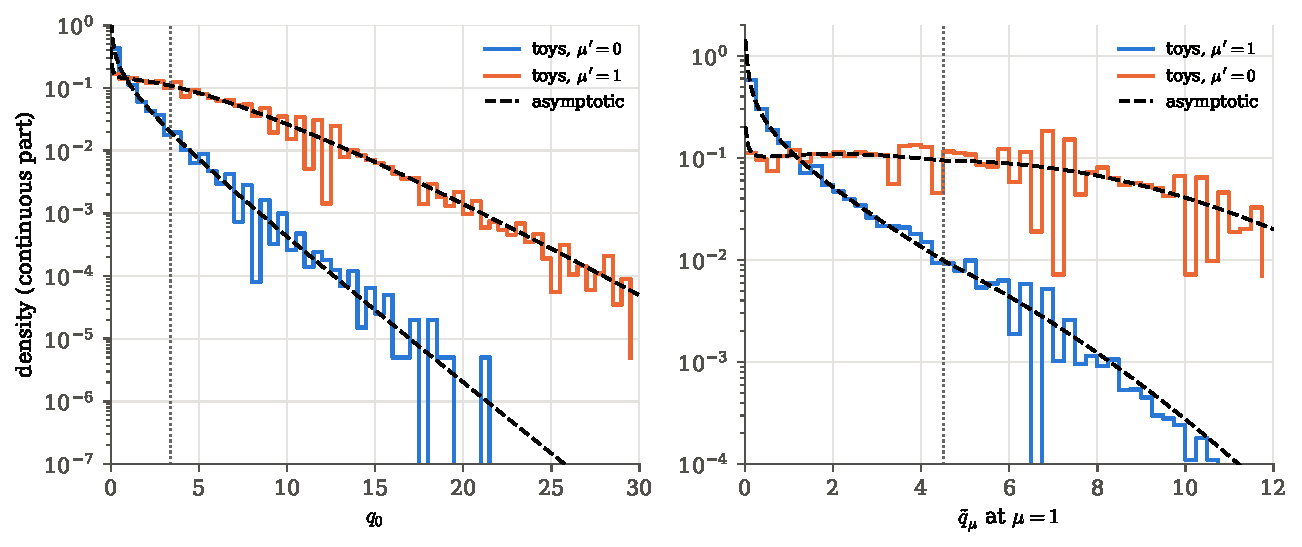
\includegraphics[width=\linewidth]{figures/ch04/hep_qdists.pdf}
\caption{Distributions of the test statistics for a counting experiment with
$s=10$, $b=10$ and a control region of the same size, from toys (steps) and from the
asymptotic formulas (dashed). Left: $q_0$ with background only (blue, the half-$\chi^2$)
and with the signal present (orange). Right: $\tilde q_\mu$ for $\mu=1$, when the
signal is present (blue, again a half-$\chi^2$) and when it is absent (orange). The
dotted lines are the Asimov values, which estimate the medians of the orange
distributions. The jagged steps come from the integer counts.}
\label{4b:fig:qdists}
\end{figure}

\subsection{The Asimov data set: what an experiment should expect}
\label{4b:sec:asimov}

Before an experiment runs, its designers want to know its \emph{sensitivity}: if the
signal is there, what significance will it typically reach, and if not, what limit
will it typically set? ``Typically'' means the median over repetitions. Simulating
thousands of experiments answers this; one artificial data set answers it too.

\begin{workdef}[Asimov data set]
The \newterm{Asimov data set} for a strength $\mu'$ is the data set in which every
count equals its expectation, $n_i=\mu's_i+b_i$, and every auxiliary measurement
equals the nominal value of its nuisance parameter \unpack{no statistical fluctuation
anywhere, the counts are allowed to be non-integer} \cite[(24)--(25)]{Cowan2011}.
\emph{Operationally:} fill the histogram with the model prediction and fit it like data.
\end{workdef}

\emph{Why do the estimators return the true values on it?} The maximum of $\ln\Like$
is where every derivative vanishes. For the Poisson part of \eqref{4b:eq:full-like},
$\ln\Like=\sum_i[n_i\ln\nu_i-\nu_i]+\text{const}$, so for any parameter $\theta_j$
(including $\mu$)
\begin{equation}
  \frac{\partial\ln\Like}{\partial\theta_j}
  \eqby{1} \sum_i\Bigl(\frac{n_i}{\nu_i}-1\Bigr)\frac{\partial\nu_i}{\partial\theta_j}
  \eqby{2} 0\quad\text{when }n_i=\nu_i\text{ for all }i,
  \label{4b:eq:asimov-score}
\end{equation}
\begin{explain}
  \item Differentiate $n_i\ln\nu_i-\nu_i$ with the chain rule.
  \item Every bracket vanishes. The Gaussian constraint terms vanish in the same way
        when $a_k=\theta_k$.
\end{explain}
So the true parameters are a maximum \cite[(23)]{Cowan2011}: fitted on the Asimov data
set, $\hat\mu=\mu'$ and $\hat{\bm\theta}=\bm\theta$.

\emph{Why does it give the median?} By \eqref{4b:eq:wald}, $q_0$ and $\tilde q_\mu$ are
monotonic functions of $\hat\mu$, and $\hat\mu$ is Gaussian with mean and median $\mu'$.
The median of a monotonic function is that function of the median. And the value of
the statistic at $\hat\mu=\mu'$ is exactly what the Asimov data set gives. So
\begin{equation}
  \mathrm{med}[Z_0\given\mu']=\sqrt{q_{0,\rm A}},
  \qquad
  \sigma_{\rm A}^2=\frac{(\mu-\mu')^2}{q_{\mu,\rm A}},
  \label{4b:eq:asimov-med}
\end{equation}
where the subscript A marks a statistic evaluated on the Asimov data set
\cite[(29)--(30), (79)]{Cowan2011}. The second formula reads \eqref{4b:eq:wald}
backwards: on the Asimov data set $\hat\mu=\mu'$, so $-2\ln\lambda_{\rm A}(\mu)=(\mu-\mu')^2/\sigma^2$
can be solved for $\sigma$. This is how the $\sigma$ in all the formulas is obtained in
practice: one fit to one artificial data set, nuisance parameters included.

\paragraph{The expected significance of a counting experiment.}
Take a count with known background $b$ and nominal signal $s$, and evaluate
$q_0=2[n\ln(n/b)-(n-b)]$ on the Asimov count $n=s+b$:
\begin{align}
  Z_{\rm A}^2=q_{0,\rm A}
  &\eqby{1} 2\Bigl[(s+b)\ln\frac{s+b}{b}-s\Bigr]
   \eqby{2} 2\Bigl[(s+b)\ln\Bigl(1+\frac sb\Bigr)-s\Bigr],
  \notag\\
  Z_{\rm A}
  &=\sqrt{2\Bigl[(s+b)\ln\Bigl(1+\frac{s}{b}\Bigr)-s\Bigr]}
   \;\relby{3}{\approx}\;\frac{s}{\sqrt b}\Bigl(1-\frac{s}{6b}\Bigr).
  \label{4b:eq:ZA}
\end{align}
\begin{explain}
  \item The known-background $q_0$ at $n=s+b$, where $n-b=s$.
  \item $(s+b)/b=1+s/b$.
  \item The expansion $q_{0,\rm A}=(s^2/b)[1-s/3b+\dots]$ worked out in the first part
        of the chapter, and $\sqrt{1-u}\approx1-u/2$.
\end{explain}
This is the same algebra as in the first part of the chapter; what is new is its
meaning, the \emph{median} significance, which \eqref{4b:eq:asimov-med} supplies. The
familiar $s/\sqrt b$ is its small-signal limit and overestimates it. For $s=b=10$,
$Z_{\rm A}=\FourBHlZAform$.

With the background measured in a control region, the Asimov counts are $n=s+b$ and
$m=\tau b$, and \eqref{4b:eq:q0-onoff} with $\hat{\hat b}(0)=(s+b+\tau b)/(1+\tau)$ gives
\begin{equation}
  Z_{\rm A}^2=2\Bigl[(s+b)\ln\frac{(1+\tau)(s+b)}{s+(1+\tau)b}
            +\tau b\ln\frac{(1+\tau)\,b}{s+(1+\tau)b}\Bigr].
  \label{4b:eq:ZA-onoff}
\end{equation}
For $s=b=10$ and $\tau=1$ this is $Z_{\rm A}=\FourBHlZA$, against $\FourBHlZAform$ with
the background known: measuring the background in a region no larger than the
signal region costs a third of the expected significance. As $\tau\to\infty$ the
control region measures $b$ perfectly: the second logarithm is
$\ln[1-s/(s+(1+\tau)b)]\approx-s/(\tau b)$, so the second term tends to $-s$, the first
to $(s+b)\ln(1+s/b)$, and \eqref{4b:eq:ZA} returns. The toys agree: their median $q_0$
under the signal is $\FourBHlMedQzero$, the same as the Asimov value $\FourBHlQzeroA$ to the digits shown. (Here the
expected counts are whole numbers, so the Asimov data set is itself a possible outcome of the experiment.)

\subsection{CL$_s$: not excluding what we cannot see}
\label{4b:sec:cls-hep}

The limit \eqref{4b:eq:mu-up} has the defect met at the start of
\cref{4b:sec:boundary}: a downward fluctuation of the background makes it negative.
There is a sharper way to see what is wrong, and it is the reason CL$_s$ exists.

\emph{The event.} An experiment with almost no sensitivity to some signal (because the
signal is tiny compared with the background, $\mu/\sigma\ll1$) reports that it
excludes that signal at $95\%$ confidence. \emph{What made it exclude?} The data
cannot tell signal from no signal, so it can only have been a downward fluctuation of
the background. \emph{How often does that happen when there is no signal?} The rule
``exclude $\mu$ if $p_\mu<\alpha$'' with $p_\mu=\Phi((\hat\mu-\mu)/\sigma)$ excludes
when $\hat\mu<\mu-\sigma\Phi^{-1}(1-\alpha)$. With background only, $\hat\mu\sim\Normal(0,\sigma^2)$:
\begin{equation}
  \Prob(\text{exclude }\mu\given0)
  \eqby{1} \Prob\Bigl(\frac{\hat\mu}{\sigma}<\frac{\mu}{\sigma}-\Phi^{-1}(1-\alpha)\Bigr)
  \eqby{2} \Phi\Bigl(\frac{\mu}{\sigma}-\Phi^{-1}(1-\alpha)\Bigr)
  \;\xrightarrow{\ \mu/\sigma\to0\ }\;\alpha .
  \label{4b:eq:blind-excl}
\end{equation}
\begin{explain}
  \item Divide the exclusion condition by $\sigma$.
  \item $\hat\mu/\sigma$ is standard normal.
\end{explain}
An experiment blind to a signal still excludes it in $5\%$ of runs. That is correct
coverage (the signal is absent, so excluding it is no error) but it is not a statement
any physicist wants to publish: the exclusion says nothing about the signal, only
about the luck of the background. The counting experiment of our toys, with a weak
signal $s=1$ on $b=10$ and $\tau=1$, has $\sigma=\FourBHlBlindSig$ at $\mu=1$; in
background-only toys it excludes $\mu=1$ in a fraction $\FourBHlExclSB$ of the runs
(the formula: $\FourBHlExclSBAsym$), not far above the $5\%$ of a completely blind
experiment, although one signal event on ten background events measured this way
is all but invisible.

\begin{workdef}[CL$_s$]
For a tested signal $\mu$ and the statistic $\tilde q_\mu$, let
$\mathrm{CL}_{s+b}=\Prob(\tilde q_\mu\ge\tilde q_{\rm obs}\given\mu)$ be the p-value of the
signal hypothesis and $\mathrm{CL}_b=\Prob(\tilde q_\mu\ge\tilde q_{\rm obs}\given0)$ the
same tail computed with background only \unpack{how background-poor the data look,
judged by the same statistic}. Then
\[
  \mathrm{CL}_s=\frac{\mathrm{CL}_{s+b}}{\mathrm{CL}_b},
\]
and $\mu$ is excluded at confidence level $1-\alpha$ if $\mathrm{CL}_s<\alpha$
\cite{Junk1999,Read2002}. In the notation of \cite{Cowan2011}, $p_\mu/(1-p_b)$.
\end{workdef}

This is the same ratio as \eqref{4b:eq:clsb} of \cref{4b:sec:fc-poisson}, where the
statistic was the count itself; the profile likelihood ratio generalises it to any
number of bins and nuisance parameters. \emph{Why does dividing help?} Take the two
extremes.
\begin{itemize}[itemsep=1pt,leftmargin=1.2em]
  \item \emph{No sensitivity.} The signal changes nothing, so both tails are computed
        from nearly the same distribution: $\mathrm{CL}_{s+b}\approx\mathrm{CL}_b$ and
        $\mathrm{CL}_s\approx1$. The signal is never excluded. In the weak-signal toys,
        CL$_s$ excluded $\mu=1$ in none of the runs (a fraction $\FourBHlExclCLs$).
  \item \emph{Good sensitivity.} Data that disfavour the signal are typical for the
        background, $\mathrm{CL}_b$ is near one, and CL$_s\approx\mathrm{CL}_{s+b}$.
        Nothing changes.
\end{itemize}
In between, dividing by $\mathrm{CL}_b\le1$ raises the ratio exactly when the data
look background-poor, which is when the plain p-value would have been lucky. The
price is over-coverage: a CL$_s$ limit is above the classical one and covers the true
value in more than $95\%$ of repetitions, as \cref{4b:fig:fc-coverage} showed for
counts. CL$_s$ is a ratio of p-values, not a p-value, and not a probability of the
signal.

\paragraph{The asymptotic CL$_s$ limit.}
By \eqref{4b:eq:p-mu}, $\mathrm{CL}_{s+b}=\Phi((\hat\mu-\mu)/\sigma)$ and, with $\mu'=0$,
$\mathrm{CL}_b=\Phi(\hat\mu/\sigma)$. The limit solves
$\mathrm{CL}_s=\alpha$:
\begin{equation}
  \Phi\Bigl(\frac{\hat\mu-\mu_{\rm up}}{\sigma}\Bigr)=\alpha\,\Phi\Bigl(\frac{\hat\mu}{\sigma}\Bigr)
  \;\Longrightarrow\;
  \mu_{\rm up}=\hat\mu+\sigma\,\Phi^{-1}\Bigl(1-\alpha\,\Phi\Bigl(\frac{\hat\mu}{\sigma}\Bigr)\Bigr),
  \label{4b:eq:cls-up}
\end{equation}
using $\Phi^{-1}(\alpha u)=-\Phi^{-1}(1-\alpha u)$. Compare \eqref{4b:eq:bayes-up} of
\cref{4b:sec:repairs}: it is the same formula. The asymptotic CL$_s$ limit on a Gaussian
estimate is the flat-prior Bayesian upper limit, just as for counts the CL$_s$ limit
equalled the flat-prior Bayesian limit \eqref{4b:eq:cls-bayes}. Two different
questions, a ratio of frequentist tails and a posterior probability with the
boundary built into the prior, give the same number. That coincidence is part of why
CL$_s$ was accepted: it behaves like a Bayesian limit near the boundary and like a
classical one far from it.

For the counting experiment with $s=b=10$, $\tau=1$ and an observation of $n=\FourBHlNobs$
events in the signal region and $m=\FourBHlMobs$ in the control region, the $95\%$
CL$_s$ limit computed with toys (tables of $\tilde q_\mu$ under $\mu$ and under $0$ on a grid
of $\mu$, $\FourBHlGridToys$ toys each) is $\mu_{\rm up}=\FourBHlLimToy$; the asymptotic
formulas, with $\sigma=\sigma_{\rm A}(\mu)$ from \eqref{4b:eq:asimov-med}, give
$\FourBHlLimAsym$.

\subsection{The expected limit and the Brazil band}
\label{4b:sec:brazil}

A limit means little without knowing what the experiment should have achieved. If
there is no signal, $\hat\mu\sim\Normal(0,\sigma^2)$, and the CL$_s$ limit
\eqref{4b:eq:cls-up} is an increasing function of $\hat\mu$. \emph{The question:} what
limit does an experiment with no signal typically report, and in what range? Since the
limit is monotonic in $\hat\mu$, its quantiles are the limits at the quantiles of
$\hat\mu$. The median is at $\hat\mu=0$; the $\pm N$ standard-deviation quantiles at
$\hat\mu=N\sigma$. Putting $\hat\mu=N\sigma$ into \eqref{4b:eq:cls-up},
\begin{equation}
  \mu_{\rm up}(N)
  \eqby{1} N\sigma+\sigma\,\Phi^{-1}\bigl(1-\alpha\,\Phi(N)\bigr),
  \qquad
  \mu_{\rm up}(0)\eqby{2}\sigma\,\Phi^{-1}(1-\alpha/2)=1.96\,\sigma ,
  \label{4b:eq:band}
\end{equation}
\begin{explain}
  \item \eqref{4b:eq:cls-up} with $\hat\mu/\sigma=N$.
  \item $\Phi(0)=\tfrac12$, and $\Phi^{-1}(0.975)=1.96$ for $\alpha=0.05$.
\end{explain}
For $N=-2,-1,0,1,2$ the bracket is $\FourBHlCoefMm$, $\FourBHlCoefM$, $\FourBHlCoefMed$,
$\FourBHlCoefP$ and $\FourBHlCoefPp$ times $\sigma$. The band is lopsided: a downward
fluctuation of the background cannot push the CL$_s$ limit much below $\sigma$, while an
upward one raises it freely. (The plain limit \eqref{4b:eq:mu-up} would have given
$1.645\sigma+N\sigma$, down to $-0.36\,\sigma$ at $N=-2$.) Since $\sigma=\sigma_{\rm A}(\mu)$
depends on the $\mu$ being tested, each line of \eqref{4b:eq:band} is solved for
$\mu_{\rm up}$ numerically \cite[(88)--(89)]{Cowan2011}.

\paragraph{Toys against Asimov.}
For the counting experiment with $s=b=10$, $\tau=1$, the script computes the CL$_s$ limit
of $\FourBHlBandToys$ background-only experiments with toys and takes the quantiles:
\begin{center}
\begin{tabular}{lccccc}
\toprule
 & $-2\sigma$ & $-1\sigma$ & median & $+1\sigma$ & $+2\sigma$\\
\midrule
toys & $\FourBHlBandToyMm$ & $\FourBHlBandToyM$ & $\FourBHlBandToyMed$ & $\FourBHlBandToyP$ & $\FourBHlBandToyPp$\\
Asimov, \eqref{4b:eq:band} & $\FourBHlBandAsMm$ & $\FourBHlBandAsM$ & $\FourBHlBandAsMed$ & $\FourBHlBandAsP$ & $\FourBHlBandAsPp$\\
\bottomrule
\end{tabular}
\end{center}
For an experiment of twenty events the asymptotic band is within a few per cent in the
middle and within ten per cent at the edges, a little conservative throughout. In
the tails the integer counts matter, and the toys are the reference.

\paragraph{The Higgs-style plots.}
For the template search of \cref{4b:sec:templates}, the script repeats the whole
procedure at every hypothesised mass from $110$ to $150\,$GeV: the observed CL$_s$
limit on $\mu$ from the pseudo-data, the expected median and bands from the Asimov
background-only data set at that mass, and the local $p_0$ with its Asimov expectation
for $\mu=1$ (\cref{4b:fig:brazil}). The green and yellow bands that give the plot its
nickname, the \newterm{Brazil band}, are \eqref{4b:eq:band}. The expected limit falls
from $\FourBHlExpLimMax$ to $\FourBHlExpLimMin$ across the range, because the background
falls with mass while the signal does not. Away from $125\,$GeV the observed limit
wanders inside the bands, as a background-only experiment should, and $\mu=1$ is
excluded at $\FourBHlNexcl$ of the $41$ masses. Near $125\,$GeV the observed limit rises far
above the band ($\FourBHlObsLimOneTwoFive$ against an expected $\FourBHlExpLimOneTwoFive$):
the data there refuse to exclude a signal, and the right panel says why. The local
significance at $125\,$GeV is $\FourBHlZlocOneTwoFive\sigma$, close to the
$\FourBHlZexpOneTwoFive\sigma$ expected for $\mu=1$. It is local: a search over this
range must correct it for the look-elsewhere effect of \cref{4b:sec:scan}.

\begin{figure}[htbp]
\centering
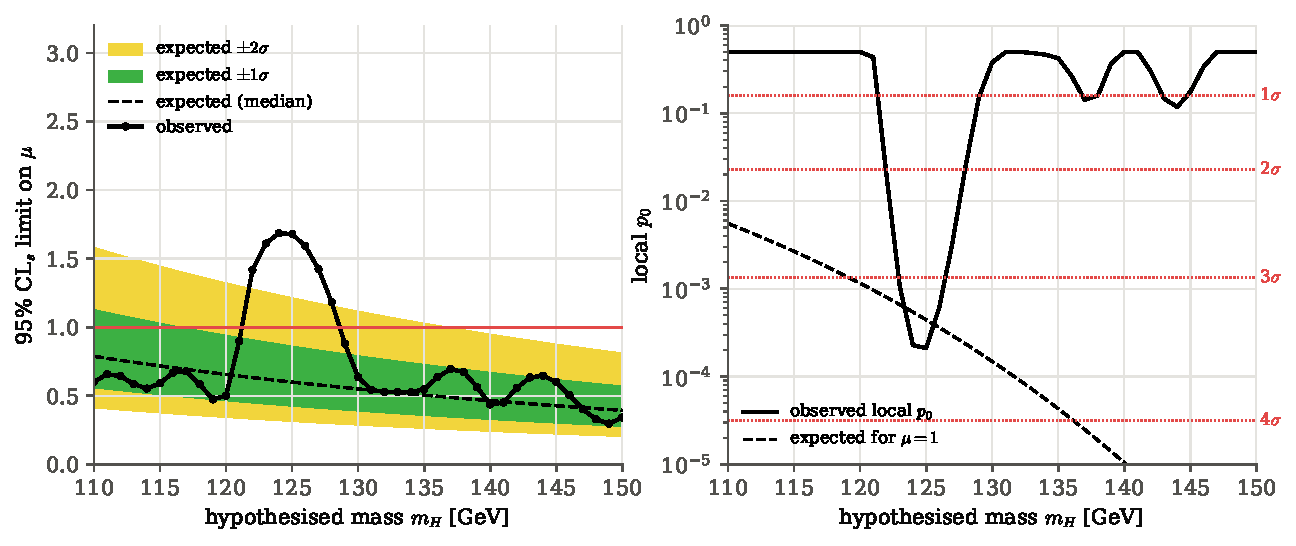
\includegraphics[width=\linewidth]{figures/ch04/hep_brazil.pdf}
\caption{The template search as the LHC experiments show it. Left: the $95\%$ CL$_s$
upper limit on the signal strength at each hypothesised mass (solid), with the median
expected for background only (dashed) and the $\pm1\sigma$ (green) and $\pm2\sigma$
(yellow) bands. Masses where the solid line is below the thin horizontal line at $\mu=1$ are
excluded for the nominal signal. Right: the local p-value of the background-only
hypothesis (solid) and its median expectation if the nominal signal is present
(dashed); the dotted lines mark $1$ to $4\sigma$.}
\label{4b:fig:brazil}
\end{figure}

\begin{keyidea}[The LHC recipe in four lines]
Write the search as a likelihood with nuisance parameters constrained by their
auxiliary measurements. Test ``no signal'' with $q_0$ and report $Z=\sqrt{q_0}$, local
and global. Exclude a signal when $\mathrm{CL}_s=\mathrm{CL}_{s+b}/\mathrm{CL}_b<0.05$, using
$\tilde q_\mu$. Show the observed limit against the expected one and its Brazil band,
both from the Asimov data set, and check with toys where counts are small.
\end{keyidea}

\begin{inpractice}[How the experiments compute it]
The likelihoods of real searches have hundreds of bins and hundreds of nuisance
parameters, with templates interpolated as in \eqref{4b:eq:morph}. They are written in
standard formats (HistFactory, with the RooStats, \texttt{pyhf} and CMS
\texttt{Combine} tools) and minimised numerically; the asymptotic formulas of
\cite{Cowan2011} give $q_0$, the CL$_s$ limit and the Brazil band from the observed and
Asimov fits alone, and toys are run where counts are small or near the boundary
\cite{Cranmer2015}. Our two scripts verify the formulas against toys on a case where
both are cheap. In research the same machinery is the instrument: the toys
are the reference whenever the formulas are in doubt, and published likelihoods let
others combine results, as \cref{4b:sec:classical-limit} urged.
\end{inpractice}

The lesson in one line: with nuisance parameters profiled, the significance is still
$\sqrt{q_0}$ and the limit still comes from a half-$\chi^2$, and CL$_s$ divides by the
background's own p-value so that a signal is never excluded by luck.
\section{Confidence intervals and credible intervals}
\label{4b:sec:credible}

Ten one-minute runs of a low-background detector record a total of six
events. Two analysts report a $90\%$ interval for the rate $\lambda$ per run.
The first, using Garwood's construction, reports $[\FourBCrConfLo,\
\FourBCrConfHi]$. The second, using Bayes' theorem with a mild prior, reports
$[\FourBCrCredLo,\ \FourBCrCredHi]$ \srcref{CasellaBerger}{Exs.~9.2.15--9.2.16}.
The numbers are close. The statements are not. The first is a confidence
interval: it comes from a recipe that covers the true rate in at least $90\%$ of
repeated experiments. The second is a \newterm{credible interval}: given these
data and the prior, it contains the rate with probability $90\%$. The first is
a prediction-direction statement, about which data each rate would produce. The
second is an inference-direction statement, about which rates could have
produced the data we saw. Bayes' theorem is the bridge between them. Comparing
the two on the same data shows what each one claims and what it needs;
\cref{ch:05} develops the Bayesian side in full.

\paragraph{The question in words.}
\begin{enumerate}[label=\arabic*.]
  \item What does each interval say, in words, and what is random in each?
  \item Does a credible interval cover like a confidence interval, and does a
        confidence interval hold the posterior probability it claims?
  \item When do the two coincide?
\end{enumerate}

\subsection{A credible set}
\label{4b:sec:credible-def}

In the Bayesian framework $\theta$ has a probability distribution, first the
prior $\pi(\theta)$ and, after the data, the posterior
$\pi(\theta\given\bm x)\propto p(\bm x\given\theta)\pi(\theta)$. Any set $A$ of
parameter values has a \newterm{credible probability}
$\Prob(\theta\in A\given\bm x)=\int_A\pi(\theta\given\bm x)\,\dd\theta$
\srcref{CasellaBerger}{(9.2.18)}, and a set with credible probability $1-\alpha$
is a $1-\alpha$ credible set. The different name keeps the two kinds of
probability apart. As with confidence intervals, many sets have the required
probability, so we must choose one.
Two common choices are the \emph{equal-tailed} interval, with posterior
probability $\alpha/2$ beyond each end, and the \newterm{highest density
interval} (HDI) \unpack{every point inside has higher posterior density than
every point outside}, which makes $\pi(a\given\bm x)=\pi(b\given\bm x)$ and is the
shortest interval with the required probability \srcref{Cowan}{(9.42)},
\srcref{Kruschke}{\S11.3.2}.

\paragraph{Example: the Poisson rate.}
Take $n$ observations from Poisson$(\lambda)$ with sum $y=\sum x_i$, and a
gamma prior with shape $a$ and scale $b$, density
$\propto\lambda^{a-1}e^{-\lambda/b}$. Then
\begin{align}
  \pi(\lambda\given\bm x)
  &\eqby{1} \propto \Bigl(\prod_{i}\lambda^{x_i}e^{-\lambda}\Bigr)\lambda^{a-1}e^{-\lambda/b}
   \eqby{2} \lambda^{a+y-1}e^{-\lambda(n+1/b)}
   \eqby{3} \mathrm{Gamma}\Bigl(a+y,\ \frac{b}{nb+1}\Bigr),
  \label{4b:eq:gamma-post}
\end{align}
\begin{explain}
  \item Bayes' theorem: likelihood of independent Poisson counts times prior;
        factors not involving $\lambda$ are dropped.
  \item Collect powers of $\lambda$ and the exponentials.
  \item This is the gamma density with shape $a+y$ and rate $n+1/b$, that is
        scale $1/(n+1/b)=b/(nb+1)$ \srcref{CasellaBerger}{(9.2.19)}.
\end{explain}
A gamma variable of shape $k$ and scale $s$, multiplied by $2/s$, is $\chi^2$
with $2k$ degrees of freedom, so $2(nb+1)\lambda/b\sim\chi^2_{2(a+y)}$ under the
posterior, and the equal-tailed interval has $\chi^2$ quantiles for ends
\srcref{CasellaBerger}{(9.2.20)}. With $a=b=1$, $n=10$, $y=6$: $22\lambda\sim\chi^2_{14}$,
and the $5\%$ and $95\%$ quantiles $6.571$ and $23.685$ give
$[\FourBCrCredLo,\FourBCrCredHi]$. The credible interval is shorter than the
confidence interval and pulled towards zero. Both effects come from the prior.
It adds information, which narrows the interval. And it favours small rates
(its density $e^{-\lambda}$ falls with $\lambda$), which pulls the interval
down.

\subsection{Judging each interval by the other's standard}
\label{4b:sec:cross-check}

Each interval keeps its own promise exactly. \emph{The question:} how does each
do when judged by the other's promise \srcref{CasellaBerger}{Ex.~9.2.17}?

\emph{Coverage of the credible interval.} Fix a true $\lambda$. Simulate the
total of the ten runs, $y\sim$ Poisson$(10\lambda)$, many times (or sum exactly
over $y$), build the credible interval each time and count hits. \Cref{4b:fig:credible-coverage}
(left) shows the result. For small $\lambda$ near the prior's bulk the credible
interval covers about $90\%$, sometimes more, sometimes less (minimum
$\FourBCrCovCredMin$ on $0<\lambda<3$). For large $\lambda$ the prior's pull
towards small values becomes a bias, and the coverage collapses: $\FourBCrCovCredFive$
at $\lambda=5$, $\FourBCrCovCredTwenty$ at $\lambda=20$, $\FourBCrCovCredFifty$ at
$\lambda=50$, tending to zero \srcref{CasellaBerger}{(9.2.22)}. A credible
interval is not a confidence interval.

\emph{Credible probability of the confidence interval.} Fix the data, compute
the posterior, and ask how much posterior probability lies inside the Garwood
interval. At $y=6$ it is $\FourBCrCredProbConfSix$; it decreases steadily with
$y$, reaching $\FourBCrCredProbConfFifty$ at $y=50$, and tends to zero for
$y\to\infty$ unless the prior scale is $b=1/n$
(\cref{4b:fig:credible-coverage}, right). A confidence interval is not a
credible interval either.

\begin{figure}[htbp]
\centering
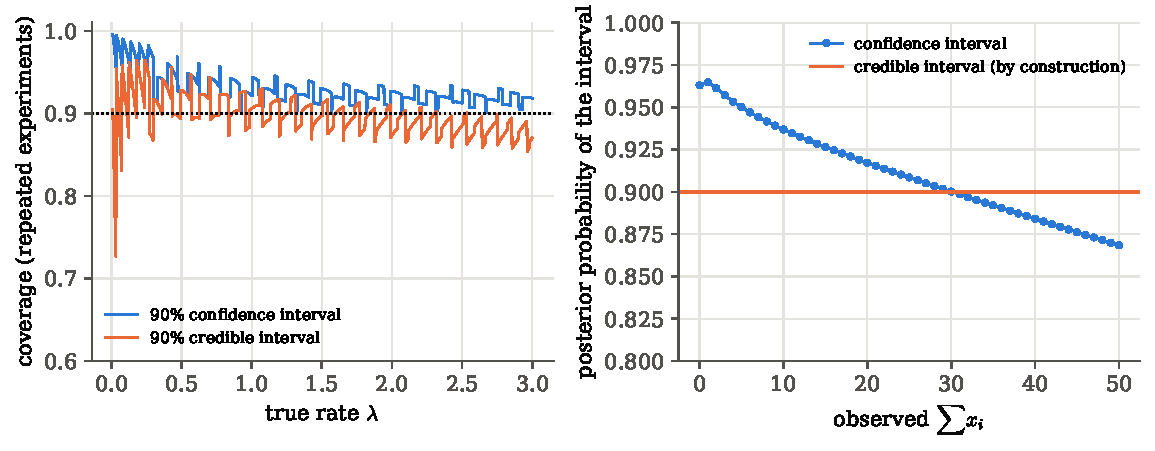
\includegraphics[width=\linewidth]{figures/ch04/credible_coverage.pdf}
\caption{Two $90\%$ intervals for a Poisson rate from ten observations,
judged by each other's criterion. Left: the frequentist coverage as a
function of the true rate. The confidence interval (blue) never drops below
$90\%$; the credible interval with a gamma$(1,1)$ prior (orange) scatters around
$90\%$ at small rates and falls away as the rate grows past the prior's range.
Right: the posterior probability contained in each interval, as a function of
the observed total. The credible interval holds $90\%$ by construction; the
confidence interval holds more for small totals and less for large ones.}
\label{4b:fig:credible-coverage}
\end{figure}

\paragraph{Example: a Gaussian mean with a Gaussian prior.}
Here the calculation can be done in closed form \srcref{CasellaBerger}{Ex.~9.2.18}.
Let $X_1,\dots,X_n$ be $\Normal(\theta,\sigma^2)$ and the prior $\Normal(\mu,\tau^2)$,
and write $\gamma=\sigma^2/(n\tau^2)$ for the ratio of the data variance of the
mean to the prior variance. The posterior is Gaussian with mean
$\delta=(\gamma\mu+\bar x)/(1+\gamma)$ and variance $V=\sigma^2/(n(1+\gamma))$, and
the $1-\alpha$ credible interval is $\delta\pm z_{\alpha/2}\sqrt V$. Its coverage at a
fixed true $\theta$, with $Z=\sqrt n(\bar X-\theta)/\sigma\sim\Normal(0,1)$ and
$\Delta=\sqrt n(\theta-\mu)/\sigma$, is
\begin{align}
  \Prob_\theta\bigl(\abs{\theta-\delta}\le z_{\alpha/2}\sqrt V\bigr)
  &\eqby{1} \Prob_\theta\Bigl(\Bigl\lvert\frac{\gamma(\theta-\mu)-(\bar X-\theta)}{1+\gamma}\Bigr\rvert
             \le z_{\alpha/2}\frac{\sigma}{\sqrt{n(1+\gamma)}}\Bigr)
   \notag\\
  &\eqby{2} \Prob\bigl(\abs{\gamma\Delta-Z}\le\sqrt{1+\gamma}\,z_{\alpha/2}\bigr)
   \notag\\
  &\eqby{3} \Phi\bigl(\gamma\Delta+\sqrt{1+\gamma}\,z_{\alpha/2}\bigr)
            -\Phi\bigl(\gamma\Delta-\sqrt{1+\gamma}\,z_{\alpha/2}\bigr).
  \label{4b:eq:normal-cred-cov}
\end{align}
\begin{explain}
  \item $\theta-\delta=[(1+\gamma)\theta-\gamma\mu-\bar X]/(1+\gamma)
        =[\gamma(\theta-\mu)-(\bar X-\theta)]/(1+\gamma)$.
  \item Multiply both sides by $(1+\gamma)\sqrt n/\sigma$ and use the
        definitions of $Z$ and $\Delta$.
  \item $Z$ is standard normal: the probability that it lies within
        $\sqrt{1+\gamma}\,z_{\alpha/2}$ of $\gamma\Delta$.
\end{explain}
So the coverage depends on how far the truth is from the prior mean, measured
by $\Delta$ in units of the standard error $\sigma/\sqrt n$. If the truth sits
at the prior mean, $\Delta=0$, the interval overcovers (for $\gamma=1$ and
$95\%$, the coverage is $\FourBCrNormCovZero$), because the prior's information
is correct. If the truth is two or four standard errors away from the prior
mean, the coverage is $\FourBCrNormCovTwo$ or $\FourBCrNormCovFour$
(\cref{4b:fig:hdi-vs-ci}, right). As $\tau\to\infty$,
$\gamma\to0$ and \eqref{4b:eq:normal-cred-cov} becomes $\Phi(z_{\alpha/2})-\Phi(-z_{\alpha/2})=1-\alpha$
for every $\theta$: with a flat prior the credible interval is the confidence
interval $\bar x\pm z_{\alpha/2}\sigma/\sqrt n$, number for number. This coincidence,
like the counting-experiment coincidence of Cowan's (9.55), is special to
location parameters and flat priors; it is why the two schools rarely argue
about a well-measured Gaussian quantity.

\subsection{The coin again: the HDI does not depend on the stopping rule}
\label{4b:sec:hdi}

Kruschke returns to $z=7$ heads in $N=24$ flips with a prior $\mathrm{beta}(11,11)$,
a coin that looks fair \srcref{Kruschke}{\S11.3.2}. The posterior is
$\mathrm{beta}(11+7,\ 11+17)$ and its $95\%$ HDI is
$[\FourBHdiInfLo,\FourBHdiInfHi]$; with a uniform prior it would be
$[\FourBHdiFlatLo,\FourBHdiFlatHi]$. \Cref{4b:fig:hdi-vs-ci} (left) shows both
posteriors with the four confidence intervals of \cref{4b:sec:ci-intentions}
underneath. The four confidence intervals differ; the HDI is the same for all
four. \emph{Why?} The Bayesian interval sees the data only through the
likelihood $\theta^7(1-\theta)^{17}$, and that is the same whether the
experimenter meant to stop at $N=24$, at $z=7$, or when time ran out. The
confidence interval also depends on which cloud of imaginary outcomes the plan
would have produced. Kruschke lists three
advantages of the HDI \srcref{Kruschke}{pp.~324--325}: it is a direct statement
about the credibility of values of $\theta$; it does not depend on sampling and
testing intentions; and it responds, openly, to prior knowledge. The price is the
prior itself, which must be stated and defended.

\begin{figure}[htbp]
\centering
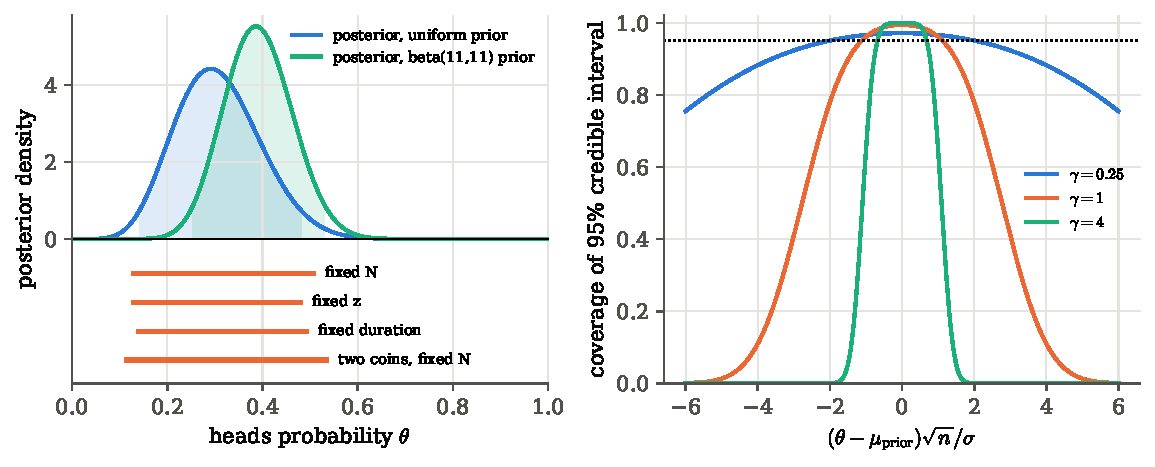
\includegraphics[width=\linewidth]{figures/ch04/hdi_vs_ci.pdf}
\caption{Left: posteriors for $7$ heads in $24$ flips with a uniform (blue) and a
$\mathrm{beta}(11,11)$ (green) prior; the shaded parts are the $95\%$ highest
density intervals. Below the axis, the four $95\%$ confidence intervals that
four stopping intentions produce from the same data. Right: frequentist coverage
of a $95\%$ credible interval for a Gaussian mean with a Gaussian prior, as a
function of the distance between the true value and the prior mean (in units of
the standard error), for three ratios $\gamma$ of data variance to prior
variance. A strong prior (large $\gamma$) covers only near its own centre.}
\label{4b:fig:hdi-vs-ci}
\end{figure}

\paragraph{Deciding with an interval: the ROPE.}
A test asks whether $\theta$ equals a null value exactly, a question whose
answer is almost always ``no'' with enough data. Kruschke replaces it by a
\newterm{region of practical equivalence} (ROPE) \unpack{a small range of values
that are, for the purpose at hand, as good as the null value}, and a rule
\srcref{Kruschke}{\S12.1.1}: reject the null value if the $95\%$ HDI lies entirely
outside the ROPE; accept it for practical purposes if the HDI lies entirely inside;
otherwise, withhold judgement. For a coin with ROPE $[0.45,0.55]$ and a uniform
prior, $325$ heads in $500$ flips give the HDI $[\FourBRopeOneLo,\FourBRopeOneHi]$,
outside the ROPE: not fair. $490$ heads in $1000$ give
$[\FourBRopeTwoLo,\FourBRopeTwoHi]$, inside: fair for practical purposes (the
posterior probability of the ROPE is $\FourBRopeTwoIn$). Unlike a p-value, this rule
can \emph{accept} a null value, and only when the measurement is precise enough to
deserve it. The physicist's analogue is familiar: a calibration is declared good
when its uncertainty band lies within the tolerance, not when a test fails to
reject perfection.

\subsection{What each interval says}
\label{4b:sec:words}

The two kinds of interval differ in what they claim, what they treat as random,
what they need as input, what they guarantee, and how they typically go wrong.

\begin{taxonomy}[Confidence interval or credible interval]
\small
\renewcommand{\arraystretch}{1.15}
\begin{tabularx}{\linewidth}{@{}>{\raggedright\arraybackslash}p{3.0cm}
                               >{\raggedright\arraybackslash}X
                               >{\raggedright\arraybackslash}X@{}}
\toprule
 & confidence interval & credible interval\\
\midrule
in words & ``a recipe that, applied to data from any $\theta$, contains that $\theta$
  $95\%$ of the time'' & ``given these data and this prior, $\theta$ is in here with
  probability $95\%$''\\
random & the interval (through the data) & $\theta$ (through the posterior)\\
fixed & the true $\theta$ & the observed data\\
needs & $p(\bm x\given\theta)$ for all data that could have occurred, including the
  stopping and search plan & the likelihood of the observed data and a prior\\
guarantee & coverage for every $\theta$ & correct posterior probability, if the prior is
  right\\
typical failure & empty or unphysical intervals, flip-flopping, dependence on
  intentions & poor coverage where the prior is wrong\\
coincide when & \multicolumn{2}{>{\raggedright\arraybackslash}X@{}}{location
  parameters with flat priors: Gaussian mean, Poisson with no background}\\
\bottomrule
\end{tabularx}
\end{taxonomy}

In the pipeline of the book, both are ways of turning the sampling
distribution $P(S\given\theta)$ of a summary into a statement about the physics.
The confidence interval stays in the prediction direction and asks which
$\theta$ would make the observed summary typical. The credible interval crosses
into the inference direction and asks how probable each $\theta$ is. Cosmologists
quote credible intervals from MCMC posteriors (\cref{ch:09}); particle physicists
quote confidence intervals and limits; the Fisher forecasts of \cref{ch:10} are,
for linear-Gaussian models, both at once. \Cref{ch:05} builds the Bayesian side
properly: priors, the evidence, and the reallocation of credibility that a posterior
is.

\begin{recap}
\begin{itemize}
  \item A $1-\alpha$ confidence interval is a recipe with coverage at least
        $1-\alpha$ for every parameter value. The interval is random, the parameter
        fixed.
  \item Inverting a family of level-$\alpha$ tests gives a $1-\alpha$ confidence
        set: keep the null values that are not rejected. The p-value function
        displays all the tests at once.
  \item The Neyman construction draws the acceptance regions of all tests as a belt
        in the (data, parameter) plane; the interval is its vertical cut. Gaussian
        estimates give $\hat\theta\pm\sigma$, Poisson counts give Garwood's
        $\chi^2$ intervals, and $\Delta\ln\Like=\tfrac12$ (or $\Delta\chi^2=1$) is
        the large-sample shortcut. With $m$ parameters the $68.3\%$ region is
        $\Delta\chi^2=2.30$ for $m=2$.
  \item Coverage is checked by simulation. Normal quantiles with an estimated
        $\sigma$ undercover at small $n$; $n\pm\sqrt n$ fails at small counts;
        discrete data force over-coverage with a saw-tooth.
  \item Near a physical boundary the classical limit can be negative or the
        interval empty. Choosing between limit and interval after seeing the data
        undercovers ($85\%$ for a nominal $90\%$). Feldman--Cousins ordering by a
        likelihood ratio fixes both; CL$_s$ (equal to the flat-prior Bayesian limit
        for counting) protects against excluding what the experiment cannot see.
  \item Many tests: Bonferroni controls the chance of any false rejection, BH the
        fraction of false discoveries. In a scan, the global p-value exceeds the
        local one by a trials factor that grows linearly with the significance;
        the Gross--Vitells formula gets it from a few toys.
  \item A credible interval is a probability statement about $\theta$ given the data
        and a prior. It does not guarantee coverage; a confidence interval does not
        hold its nominal posterior probability; they agree for flat priors on location
        parameters.
\end{itemize}
\end{recap}

\subsection*{Reading the literature}
\label{4b:sec:literature}

\begin{itemize}[leftmargin=1.2em,itemsep=2pt]
  \item \textbf{Main line.} \mainref{Ch.~10} for hypothesis testing: the null and
        the alternative, power and size, the Wald test, p-values and their
        uniformity, the $\chi^2$ and permutation tests, likelihood-ratio tests,
        multiple testing (Bonferroni and Benjamini--Hochberg) and goodness of fit;
        \mainref{\S6.3.2} for confidence sets, their interpretation and the
        Berger--Wolpert example.
  \item \textbf{The physicist's version.} \srcref{Cowan}{Ch.~4} for test statistics,
        particle selection, the Neyman--Pearson lemma, goodness of fit and the
        significance of a signal; \srcref{Cowan}{Ch.~9} for confidence belts,
        Gaussian and Poisson intervals, Fisher's $z$, likelihood intervals,
        confidence regions and limits near a boundary, with and without background.
  \item \textbf{Careful derivations.} \srcref{CasellaBerger}{\S8.3} for the
        Neyman--Pearson lemma and valid p-values; \srcref{CasellaBerger}{\S10.3}
        for the asymptotic distribution of the likelihood ratio;
        \srcref{CasellaBerger}{\S\S9.1--9.2} for interval estimators, coverage and
        confidence coefficients, test inversion, pivots, Garwood's Poisson
        intervals and the coverage of credible sets.
  \item \textbf{The Bayesian critique.} \srcref{Kruschke}{Ch.~11} for how p-values
        and confidence intervals depend on stopping and testing intentions, and for
        multiple comparisons; \srcref{Kruschke}{Ch.~12} for the HDI and the region of
        practical equivalence. \srcref{Lambert}{\S2.8} for the frequentist's
        imaginary samples.
  \item \textbf{Original papers.} Feldman and Cousins' unified approach to small
        signals \cite{FeldmanCousins1998}; Gross and Vitells on trials factors for
        the look-elsewhere effect \cite{GrossVitells2010}; Cowan, Cranmer, Gross and
        Vitells on asymptotic formulae for likelihood-based tests of new physics,
        including the profile likelihood ratio, the Asimov data set and the CL$_s$
        remark \cite{Cowan2011}; Wilks on the asymptotic $\chi^2$ distribution of
        likelihood ratios \cite{Wilks1938}.
\end{itemize}

\clearpage
\raggedbottom
\section*{Chapter summary}
\addcontentsline{toc}{section}{Chapter summary}
\label{4b:sec:summary}

Before a measurement is published it must answer three questions. Could this be
chance? Which parameter values are compatible with what we saw? How often do
our recipes mislead us? All three start from the sampling distribution of a
summary. Tests answer the first: they are built around the one hypothesis
whose predictions we know, the null, and measure surprise with p-values.
Intervals and limits answer the second: they are families of tests, inverted.
Coverage checks and corrections for the many places we looked answer the third.
In the pipeline of the book,
\[
  \text{model}\to\text{data}\to\text{summary }S\to P(S\given\theta)\to\boxed{\text{infer physics}},
\]
tests and intervals are the frequentist form of the last arrow, and
\cref{ch:05} gives the Bayesian one.

\begin{center}
\small
\renewcommand{\arraystretch}{1.15}
\begin{tabularx}{\linewidth}{@{}>{\raggedright\arraybackslash}p{3.3cm}
                               >{\raggedright\arraybackslash}X
                               >{\raggedright\arraybackslash}p{2.7cm}@{}}
\toprule
\multicolumn{3}{@{}l}{\textbf{Testing the null (first half)}}\\
concept & operational meaning & used later in\\\midrule
null hypothesis & the hypothesis whose sampling distribution we know and can simulate: ``it happened by chance'' & every search, \cref{ch:08,ch:12}\\
test statistic, rejection region & one number, large under the alternative; reject when it exceeds a critical value fixed in advance & \cref{ch:08,ch:12}\\
p-value & probability under $\Hnull$ of a statistic at least as extreme, in the alternative's direction; simulate if no formula & \cref{ch:06,ch:08,ch:12}\\
one- and two-sided, stopping rule & the direction and the experimental plan are part of the question; they change the p-value & \cref{ch:05}\\
size, power & false-alarm rate $\alpha$; rejection probability under the truth; plan the experiment by the power & \cref{ch:10}\\
uniformity of p & under a continuous null $p\sim\mathrm{U}(0,1)$; for discrete data $\Prob(p\le\alpha)\le\alpha$; a histogram of null p-values checks a pipeline & \cref{ch:06,ch:08}\\
$p\ne\Prob(\Hnull\given\text{data})$ & the posterior of the null needs a prior and the power (Bayes) & \cref{ch:05}\\
Wald, $t$, permutation tests & estimate over standard error; Student $t$ for small Gaussian samples; relabel the data for a distribution-free null & \cref{ch:06,ch:12}\\
Neyman--Pearson, likelihood ratio & for simple hypotheses the likelihood ratio is the most powerful statistic & \cref{ch:08,ch:10}\\
Wilks, $q_0$, $Z=\sqrt{q_0}$ & $-2\ln\lambda\sim\chi^2$ with as many degrees of freedom as the null fixes; half-$\chi^2$ on a boundary & \cref{ch:09,ch:10}\\
Pearson $\chi^2$, KS & goodness of fit of a whole model; fitted parameters reduce the degrees of freedom; simulate sparse cases & \cref{ch:07,ch:08}\\
$p\to Z\sigma$, $5\sigma$ & $Z=\Phi^{-1}(1-p)$; $3\sigma$ evidence, $5\sigma$ observation, because of many searches, backgrounds and rarity & \cref{ch:12}\\
\bottomrule
\end{tabularx}
\end{center}

\begin{center}
\small
\renewcommand{\arraystretch}{1.15}
\begin{tabularx}{\linewidth}{@{}>{\raggedright\arraybackslash}p{3.3cm}
                               >{\raggedright\arraybackslash}X
                               >{\raggedright\arraybackslash}p{2.7cm}@{}}
\toprule
\multicolumn{3}{@{}l}{\textbf{Intervals, coverage and many tests (second half)}}\\
concept & operational meaning & used later in\\\midrule
confidence interval & a recipe with coverage $\ge1-\alpha$ for every $\theta$; the interval is random, $\theta$ fixed & \cref{ch:08,ch:10}\\
test inversion, p-value function & keep the null values a level-$\alpha$ test does not reject & \cref{ch:08}\\
Neyman belt & acceptance intervals at every $\theta$, cut vertically at the observation; build on a grid from simulations when there is no formula & \cref{ch:06,ch:08}\\
Gaussian and Poisson intervals & $\hat\theta\pm\sigma$ is the $68.3\%$ central interval; Garwood's $\chi^2$ quantiles for counts; $-\ln0.05=3$ for zero events & \cref{ch:07,ch:08}\\
likelihood interval, $\Delta\chi^2$ regions & $\Delta\ln\Like=\tfrac12$, $\Delta\chi^2=1$ in one dimension; $2.30$ ($68.3\%$) and $5.99$ ($95\%$) in two & \cref{ch:09,ch:10}\\
coverage check & simulate at fixed $\theta$, count hits; exact sums for counts; $t$ not $z$ for estimated $\sigma$ & \cref{ch:06,ch:08,ch:09}\\
limits near a boundary & report $\hat\theta\pm\sigma$ always; classical, shifted, Bayesian, Feldman--Cousins, CL$_s$; fix the recipe in advance & \cref{ch:10}\\
Bonferroni, BH & $P_i<\alpha/m$ controls any false rejection; the BH line $i\alpha/m$ controls the false discovery rate & \cref{ch:12}\\
look-elsewhere effect & global p-value from toys scanned like the data; $p_{\rm glob}\approx p_{\rm loc}+\E N(c_0)e^{-(c-c_0)/2}$; trials factor $\propto Z$ & \cref{ch:08,ch:12}\\
search likelihood, nuisance parameters & Poisson bins of signal and background templates times one constraint term per calibration; profile to get $\lambda(\mu)$; $\sigma_{\rm syst}^2=\sigma_{\rm tot}^2-\sigma_{\rm stat}^2$ & \cref{ch:08,ch:10}\\
$q_0$, $\tilde q_\mu$, CL$_s$, Brazil band & $Z=\sqrt{q_0}$ with profiled nuisances (Wald); exclude when $\mathrm{CL}_{s+b}/\mathrm{CL}_b<0.05$; expected limit and $\pm1,2\sigma$ bands from the Asimov data set; toys for small counts & \cref{ch:10,ch:12}\\
credible interval, HDI, ROPE & posterior probability of a set given data and prior; shortest set; accept or reject a value for practical purposes & \cref{ch:05,ch:09}\\
\bottomrule
\end{tabularx}
\end{center}
\clearpage
\flushbottom
  